% ******************************* PhD Thesis Template **************************
% Please have a look at the README.md file for info on how to use the template

\documentclass[a4paper,12pt,times,numbered,print,index]{Classes/PhDThesisPSnPDF}

% ******************************************************************************
% ******************************* Class Options ********************************
% *********************** See README for more details **************************
% ******************************************************************************

% `a4paper'(The University of Cambridge PhD thesis guidelines recommends a page
% size a4 - default option) or `a5paper': A5 Paper size is also allowed as per
% the Cambridge University Engineering Deparment guidelines for PhD thesis
%
% `11pt' or `12pt'(default): Font Size 10pt is NOT recommended by the University
% guidelines
%
% `oneside' or `twoside'(default): Printing double side (twoside) or single
% side.
%
% `print': Use `print' for print version with appropriate margins and page
% layout. Leaving the options field blank will activate Online version.
%
% `index': For index at the end of the thesis
%
% `draftclassic': For draft mode without loading any images (same as draft in book)
%
% `draft': Special draft mode with line numbers, images, and water mark with
% timestamp and custom text. Position of the text can also be modified.
%
% `abstract': To generate only the title page and abstract page with
% dissertation title and name, to submit to the Student Registry
%
% `chapter`: This option enables only the specified chapter and it's references
%  Useful for review and corrections.
%
% ************************* Custom Page Margins ********************************
%
% `custommargin`: Use `custommargin' in options to activate custom page margins,
% which can be defined in the preamble.tex. Custom margin will override
% print/online margin setup.
%
% *********************** Choosing the Fonts in Class Options ******************
%
% `times' : Times font with math support. (The Cambridge University guidelines
% recommend using times)
%
% `fourier': Utopia Font with Fourier Math font (Font has to be installed)
%            It's a free font.
%
% `customfont': Use `customfont' option in the document class and load the
% package in the preamble.tex
%
% default or leave empty: `Latin Modern' font will be loaded.
%
% ********************** Choosing the Bibliography style ***********************
%
% `authoryear': For author-year citation eg., Krishna (2013)
%
% `numbered': (Default Option) For numbered and sorted citation e.g., [1,5,2]
%
% `custombib': Define your own bibliography style in the `preamble.tex' file.
%              `\RequirePackage[square, sort, numbers, authoryear]{natbib}'.
%              This can be also used to load biblatex instead of natbib
%              (See Preamble)
%
% **************************** Choosing the Page Style *************************
%
% `default (leave empty)': For Page Numbers in Header (Left Even, Right Odd) and
% Chapter Name in Header (Right Even) and Section Name (Left Odd). Blank Footer.
%
% `PageStyleI': Chapter Name next & Page Number on Even Side (Left Even).
% Section Name & Page Number in Header on Odd Side (Right Odd). Footer is empty.
%
% `PageStyleII': Chapter Name on Even Side (Left Even) in Header. Section Number
% and Section Name in Header on Odd Side (Right Odd). Page numbering in footer

\newtheorem{theorem}{Theorem}[section]
\newtheorem{lemma}[theorem]{Lemma}
\newtheorem{hypothesis}[theorem]{$\mathcal{H}$}
\newtheorem{proposition}[theorem]{Proposition}
\newtheorem{corollary}[theorem]{Corollary}

\newenvironment{proof}[1][Proof]{\begin{trivlist}
\item[\hskip \labelsep {\bfseries #1}]}{\end{trivlist}}
\newenvironment{definition}[1][Definition]{\begin{trivlist}
\item[\hskip \labelsep {\bfseries #1}]}{\end{trivlist}}
\newenvironment{example}[1][Example]{\begin{trivlist}
\item[\hskip \labelsep {\bfseries #1}]}{\end{trivlist}}
\newenvironment{remark}[1][Remark]{\begin{trivlist}
\item[\hskip \labelsep {\bfseries #1}]}{\end{trivlist}}

% tombstones for the end of proof
\newcommand{\qed}{\nobreak \ifvmode \relax \else
      \ifdim\lastskip<1.5em \hskip-\lastskip
      \hskip1.5em plus0em minus0.5em \fi \nobreak
      \vrule height0.75em width0.5em depth0.25em\fi}

\newcommand\hyptref[1]{$\mathcal{H}$[\ref{#1}]}
\newcommand\propref[1]{$\mathcal{P}$[\ref{#1}]}
\newcommand\prop[1]{(\mathcal{P}_{#1})}




% ********************************** Preamble **********************************
% Preamble: Contains packages and user-defined commands and settings
% ******************************************************************************
% ****************************** Custom Margin *********************************

% Add `custommargin' in the document class options to use this section
% Set {innerside margin / outerside margin / topmargin / bottom margin}  and
% other page dimensions
\ifsetCustomMargin
  \RequirePackage[left=37mm,right=30mm,top=35mm,bottom=30mm]{geometry}
  \setFancyHdr % To apply fancy header after geometry package is loaded
\fi

% ******************************************************************************
% ****************************** Allow space at bottom of page *********************************
\raggedbottom

% *****************************************************************************
% ******************* Fonts (like different typewriter fonts etc.)*************

% Add `customfont' in the document class option to use this section

\ifsetCustomFont
  % Set your custom font here and use `customfont' in options. Leave empty to
  % load computer modern font (default LaTeX font).
  %\RequirePackage{helvet}

  % For use with XeLaTeX
  %  \setmainfont[
  %    Path              = ./libertine/opentype/,
  %    Extension         = .otf,
  %    UprightFont = LinLibertine_R,
  %    BoldFont = LinLibertine_RZ, % Linux Libertine O Regular Semibold
  %    ItalicFont = LinLibertine_RI,
  %    BoldItalicFont = LinLibertine_RZI, % Linux Libertine O Regular Semibold Italic
  %  ]
  %  {libertine}
  %  % load font from system font
  %  \newfontfamily\libertinesystemfont{Linux Libertine O}
\fi

% *****************************************************************************
% **************************** Custom Packages ********************************

% ************************* Algorithms and Pseudocode **************************

\usepackage{amsmath}
\usepackage{empheq}
\usepackage{amssymb}
\usepackage{algorithm}
\usepackage{algpseudocode}
\usepackage{graphicx}
\usepackage{float}
\usepackage{placeins}
%\usepackage{url}
\usepackage{color}
\usepackage{flushend}
\usepackage{overpic}
\usepackage[table]{xcolor}
\usepackage{multirow}
%\usepackage{ulem}
\usepackage{natbib}
\usepackage{bibentry}
\nobibliography*

\usepackage{pgfplots}
\usepackage[utf8]{inputenc}

\usepackage{tikz}
\usetikzlibrary{shapes.geometric, arrows}

\pgfplotsset{compat=1.9}

%\usepgfplotslibrary{external}
%\tikzexternalize

%\usepackage[colorlinks = true,
            %linkcolor = blue,
            %urlcolor  = blue,
            %citecolor = blue,
            %anchorcolor = blue]{hyperref}
%\newcommand{\colorhref}[3][blue]{\href{#2}{\color{#1}{#3}}}%
\usepackage{hyperref}
% ********************Captions and Hyperreferencing / URL **********************

% Captions: This makes captions of figures use a boldfaced small font.
%\RequirePackage[small,bf]{caption}

\RequirePackage[labelsep=space,tableposition=top]{caption}
\renewcommand{\figurename}{Fig.} %to support older versions of captions.sty


% *************************** Graphics and figures *****************************

%\usepackage{rotating}
%\usepackage{wrapfig}

% Uncomment the following two lines to force Latex to place the figure.
% Use [H] when including graphics. Note 'H' instead of 'h'
%\usepackage{float}
%\restylefloat{figure}

% Subcaption package is also available in the sty folder you can use that by
% uncommenting the following line
% This is for people stuck with older versions of texlive
%\usepackage{sty/caption/subcaption}
\usepackage{subcaption}

% ********************************** Tables ************************************
\usepackage{booktabs} % For professional looking tables
\usepackage{multirow}

%\usepackage{multicol}
%\usepackage{longtable}
%\usepackage{tabularx}


% *********************************** SI Units *********************************
\usepackage{siunitx} % use this package module for SI units


% ******************************* Line Spacing *********************************

% Choose linespacing as appropriate. Default is one-half line spacing as per the
% University guidelines

% \doublespacing
% \onehalfspacing
% \singlespacing


% ************************ Formatting / Footnote *******************************

% Don't break enumeration (etc.) across pages in an ugly manner (default 10000)
%\clubpenalty=500
%\widowpenalty=500

%\usepackage[perpage]{footmisc} %Range of footnote options


% *****************************************************************************
% *************************** Bibliography  and References ********************

%\usepackage{cleveref} %Referencing without need to explicitly state fig /table

% Add `custombib' in the document class option to use this section
\ifuseCustomBib
   \RequirePackage[square, sort, numbers, authoryear]{natbib} % CustomBib

% If you would like to use biblatex for your reference management, as opposed to the default `natbibpackage` pass the option `custombib` in the document class. Comment out the previous line to make sure you don't load the natbib package. Uncomment the following lines and specify the location of references.bib file

%\RequirePackage[backend=biber, style=numeric-comp, citestyle=numeric, sorting=nty, natbib=true]{biblatex}
%\bibliography{References/references} %Location of references.bib only for biblatex

\fi

% changes the default name `Bibliography` -> `References'
\renewcommand{\bibname}{References}


% ******************************** Roman Pages *********************************
% The romanpages environment set the page numbering to lowercase roman one
% for the contents and figures lists. It also resets
% page-numbering for the remainder of the dissertation (arabic, starting at 1).

\newenvironment{romanpages}{
  \setcounter{page}{1}
  \renewcommand{\thepage}{\roman{page}}}
{\newpage\renewcommand{\thepage}{\arabic{page}}}


% ******************************************************************************
% ************************* User Defined Commands ******************************
% ******************************************************************************

% *********** To change the name of Table of Contents / LOF and LOT ************

%\renewcommand{\contentsname}{My Table of Contents}
%\renewcommand{\listfigurename}{My List of Figures}
%\renewcommand{\listtablename}{My List of Tables}

\def\note{\textcolor{red}}

\newcommand{\Figref}[2]{Fig.~\ref{#1}#2}
\newcommand{\Eqref}[1]{(\ref{#1})}
\newcommand{\compare}[2]{\textcolor{red}{#1} \textcolor{blue}{#2}}
\newcommand{\diff}[2]{\dfrac{\partial #1}{\partial #2}}
\newcommand{\norm}[1]{\left\| #1 \right\|}
\newcommand{\reduce}[2]{\hspace{-#2pt} #1 \hspace{-#2pt}}
\newcommand{\ipspace}{\mathfrak{P}}
\DeclareMathOperator*{\minimize}{min.}
\DeclareMathOperator{\plog}{plog}
\DeclareMathOperator{\dist}{dist}
\DeclareMathOperator*{\argmin}{arg\ min.}

% Reset MathCal to default
\DeclareMathAlphabet{\mathcal}{OMS}{cmsy}{m}{n}

% define widecheck
%% code from mathabx.sty and mathabx.dcl
\DeclareFontFamily{U}{mathx}{\hyphenchar\font45}
\DeclareFontShape{U}{mathx}{m}{n}{
      <5> <6> <7> <8> <9> <10>
      <10.95> <12> <14.4> <17.28> <20.74> <24.88>
      mathx10
      }{}
\DeclareSymbolFont{mathx}{U}{mathx}{m}{n}
\DeclareFontSubstitution{U}{mathx}{m}{n}
\DeclareMathAccent{\widecheck}{0}{mathx}{"71}
\DeclareMathAccent{\wideparen}{0}{mathx}{"75}

\def\cs#1{\texttt{\char`\\#1}}
% ********************** TOC depth and numbering depth *************************

\setcounter{secnumdepth}{2}
\setcounter{tocdepth}{2}


% ******************************* Nomenclature *********************************

% To change the name of the Nomenclature section, uncomment the following line

\renewcommand{\nomname}{Symbols}
\usepackage{etoolbox}
\renewcommand\nomgroup[1]{%
  \item[\bfseries
  \ifstrequal{#1}{S}{Spaces}{%
  \ifstrequal{#1}{N}{Number Sets}{%
  \ifstrequal{#1}{Z}{Abbreviations/Acronyms}{%
  \ifstrequal{#1}{R}{Robotics-related Symbols}{%
  \ifstrequal{#1}{P}{Optimization-related Symbols}{%
  \ifstrequal{#1}{X}{Other Symbols}{%
  \ifstrequal{#1}{O}{Operators}{}}}}}}}%
]}
% ********************************* Appendix ***********************************

% The default value of both \appendixtocname and \appendixpagename is `Appendices'. These names can all be changed via:

%\renewcommand{\appendixtocname}{List of appendices}
%\renewcommand{\appendixname}{Appndx}

% *********************** Configure Draft Mode **********************************

% Uncomment to disable figures in `draftmode'
%\setkeys{Gin}{draft=true}  % set draft to false to enable figures in `draft'

% These options are active only during the draft mode
% Default text is "Draft"
%\SetDraftText{DRAFT}

% Default Watermark location is top. Location (top/bottom)
%\SetDraftWMPosition{bottom}

% Draft Version - default is v1.0
%\SetDraftVersion{v1.1}

% Draft Text grayscale value (should be between 0-black and 1-white)
% Default value is 0.75
%\SetDraftGrayScale{0.8}


% ******************************** Todo Notes **********************************
%% Uncomment the following lines to have todonotes.

%\ifsetDraft
%	\usepackage[colorinlistoftodos]{todonotes}
%	\newcommand{\mynote}[1]{\todo[author=kks32,size=\small,inline,color=green!40]{#1}}
%\else
%	\newcommand{\mynote}[1]{}
%	\newcommand{\listoftodos}{}
%\fi

% Example todo: \mynote{Hey! I have a note}


% ************************ Thesis Information & Meta-data **********************
% Thesis title and author information, refernce file for biblatex
% ************************ Thesis Information & Meta-data **********************
%% The title of the thesis
\title{Numerical optimization on non-Euclidean manifolds and its use in robotics posture generation}
%\texorpdfstring is used for PDF metadata. Usage:
%\texorpdfstring{LaTeX_Version}{PDF Version (non-latex)} eg.,
%\texorpdfstring{$sigma$}{sigma}

%% Subtitle (Optional)
%\subtitle{Using the CUED template}

%% The full name of the author
\author{Stanislas Brossette}

%% Department (eg. Department of Engineering, Maths, Physics)
\dept{Department of Engineering}

%% University and Crest
\university{Université de Montpellier}
% Crest minimum should be 30mm.
\crest{
\includegraphics[width=0.2\textwidth]{University_of_Montpellier_seal.png}}
%% Use this crest, if you are using the college crest
%% Crest long miminum should be 65mm
%\crest{\includegraphics[width=0.45\textwidth]{University_Crest_Long}}

%% College shield [optional] 
% Crest minimum should be 30mm.
%\collegeshield{\includegraphics[width=0.2\textwidth]{CollegeShields/Kings}}

%% You can redefine the submission text:
% Default as per the University guidelines:
% ``This dissertation is submitted for the degree of''
%\renewcommand{\submissiontext}{change the default text here if needed}

%% Full title of the Degree
\degreetitle{Doctor of Philosophy}

%% College affiliation (optional)
%\college{King's College}

%% Submission date
% Default is set as {\monthname[\the\month]\space\the\year}
%\degreedate{September 2014} 

%% Meta information
\subject{LaTeX} \keywords{{LaTeX} {PhD Thesis} {Engineering} {University of
Cambridge}}


% ***************************** Abstract Separate ******************************
% To printout only the titlepage and the abstract with the PhD title and the
% author name for submission to the Student Registry, use the `abstract' option in
% the document class.

% Multi-language abstract
\usepackage[francais,english]{babel}
\usepackage{csquotes}

\ifdefineAbstract
 \pagestyle{empty}
 \includeonly{Declaration/declaration, Abstract/abstract}
\fi
% Renew for abstract with multiple languages
\newenvironment{abstractpage}
  {\cleardoublepage\vspace*{\fill}\thispagestyle{empty}}
  {\vfill\cleardoublepage}
\renewenvironment{abstract}[1]{%
  % Normal abstract in the thesis
  \setsinglecolumn%
  \bigskip\selectlanguage{#1}%
  \section*{\centering \Large \abstractname}
  \thispagestyle{empty}
}

% ***************************** Chapter Mode ***********************************
% The chapter mode allows user to only print particular chapters with references
% Title, Contents, Frontmatter are disabled by default
% Useful option to review a particular chapter or to send it to supervisior.
% To use choose `chapter' option in the document class

\ifdefineChapter
 \includeonly{Chapter3/chapter3}
\fi


% ******************************** Front Matter ********************************
\usepackage{pdfpages}

\begin{document}

\frontmatter
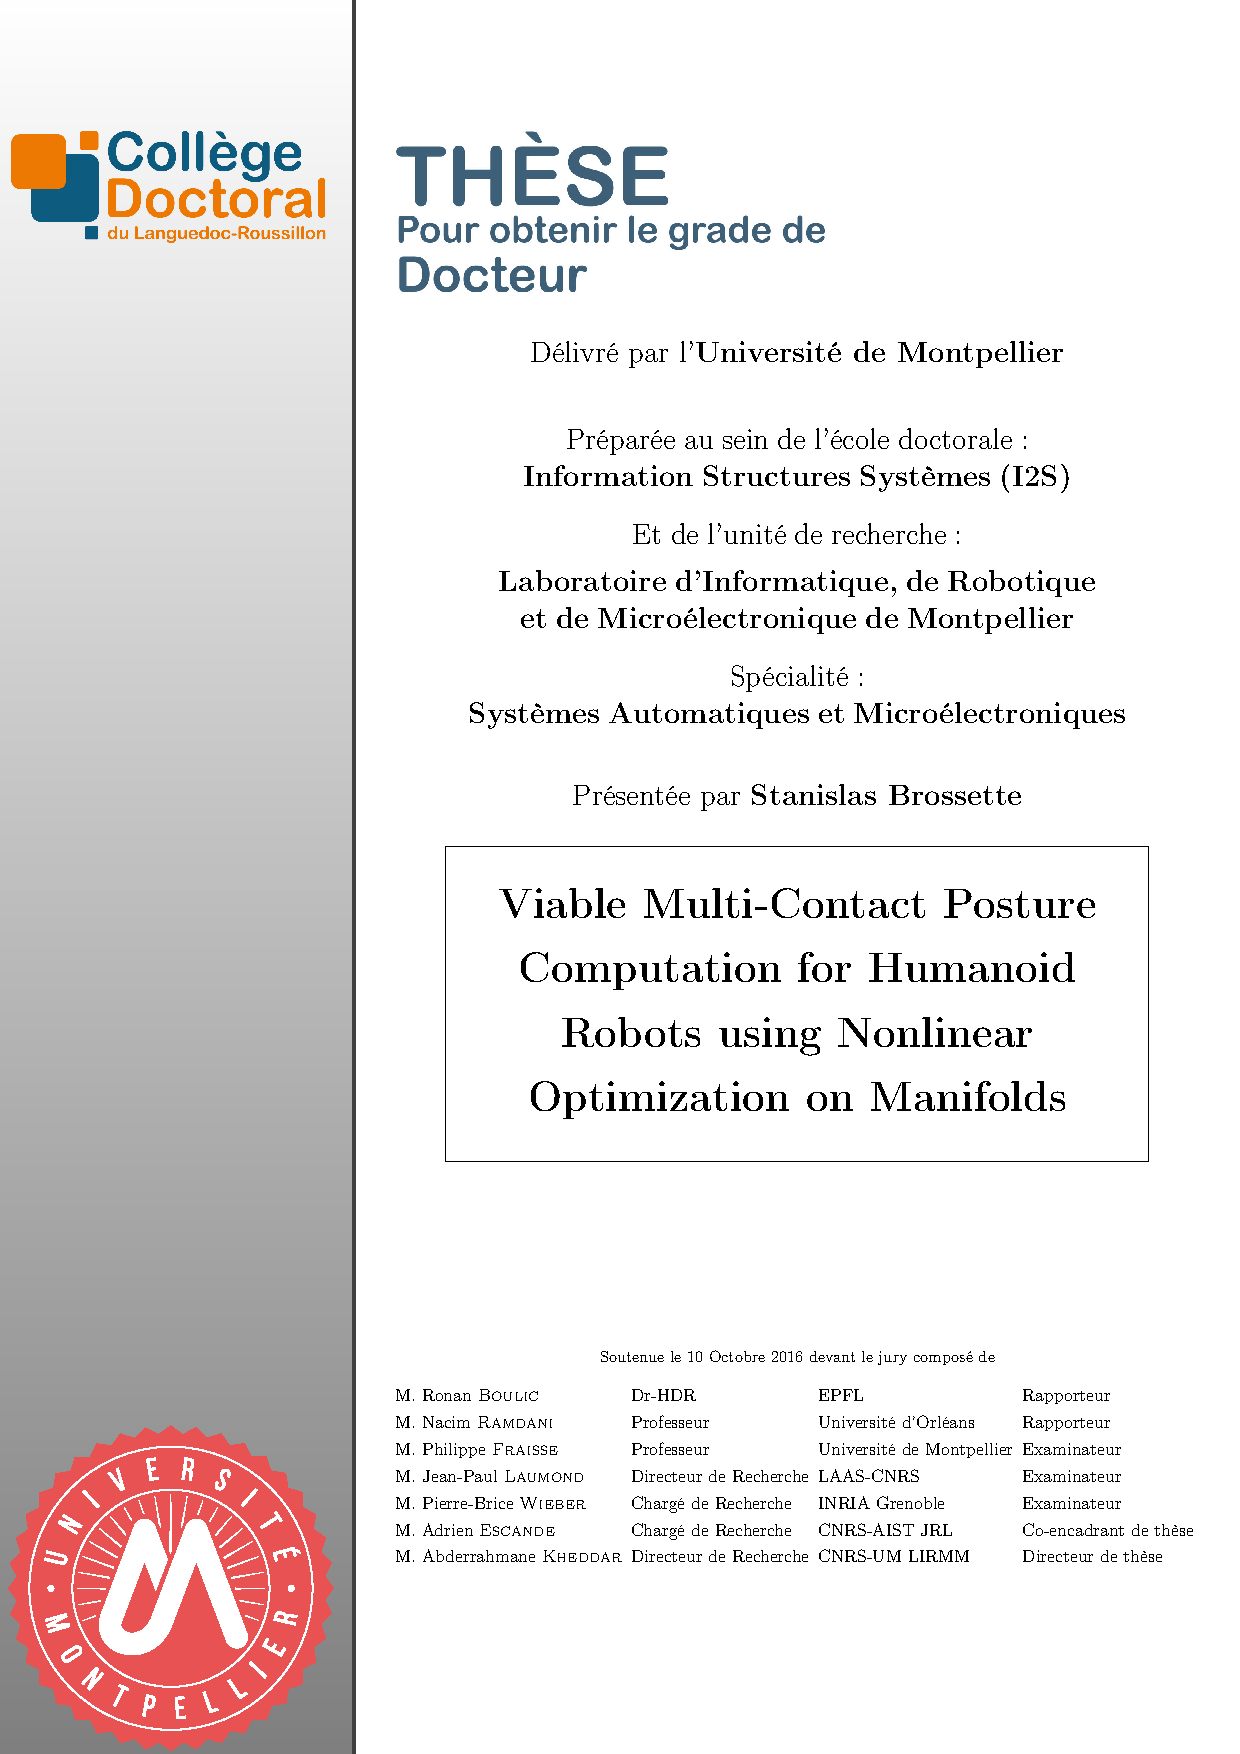
\includepdf[pages=-]{Cover/build/cover}

%\begin{titlepage}
  %\maketitle
%\end{titlepage}


\include{Dedication/dedication}
\include{Declaration/declaration}
% ************************** Thesis Acknowledgements **************************

\begin{acknowledgements}

I would like to thank my Ph.D supervisor, Abderrahmane Kheddar, for giving me the opportunity to work in his team, and for his advices and support all along the course of my Ph.D.

I am very thankful to my Ph.D co-supervisor, Adrien Escande, without whom this work would never have gone this far.
Thank you for your precious advices, for your support, and for your patience.

It is a great honor for me to have Ronan Boulic and Nacim Ramdani review this dissertation, and to have this thesis examined by Philippe Fraisse, Jean-Paul Laumond and Pierre-Brice Wieber.

I would like to thank the AIST and Eiichi Yoshida for hosting me in Japan.

I express my gratitude to Oskar von Stryk from Darmstadt University for giving me the opportunity to participate with their team in the pre-finals DARPA Robotics Challenge, and to Francesco Nori for giving me the opportunity to explore a new application of my work.

I would like to thank and acknowledge several people with whom I interacted, had fruitful conversations, and who helped me in different ways during this work:
Herv\'e Audren,
Benjamin Chr\'etien,
Gr\'egoire Duchemin,
Giovanni De Magistris,
Gowrishankar Ganesh,
Pierre Gergondet,
Francois Keith,
Thomas Moulard and
Joris Vaillant.

I am very thankful to my family, for supporting me, motivating me and believing in me all this time.

Finally, I would like to dedicate this thesis to my unconditionally loving girlfriend, Airi Nakajima, and to thank her for her patience and priceless support all along this Ph.D.

\end{acknowledgements}

% ************************** Thesis Abstract *****************************
% Use `abstract' as an option in the document class to print only the titlepage and the abstract.
\begin{abstractpage}
  \vspace{-5em}
  \begin{abstract}{english}
    Humanoid robots are complex poly-articulated structures with non-linear kinematics and dynamics.
    Finding viable postures to realize set-point task objectives under a set of constraints (intrinsic and extrinsic limitations) is a key issue in the planning of robot motion and an important feature of any robotics framework.
    It is handled by the so called posture generator (PG) that consists in formalizing the viable posture as the solution of a nonlinear optimization problem.
    We present several extensions to the state-of-the-art by exploring new formulations and resolution methods for posture generation problems.
    We reformulate the notion of contact constraints by adding variables to enrich the optimization problem and allow the solver to decide the shape of intersection of contact polygons, or of the location of a contact point on a non-flat surface.
    We present a reformulation of the posture generation problem that encompasses non-Euclidean manifolds natively, and presents a more elegant and efficient mathematical formulation of it.
    To solve such problems, we implemented a new SQP solver that is particularly suited to handle non-Euclidean manifolds structures.
    By doing so, we have a better mastering in the way to tune and specialize our solver for robotics problems.

    \textbf{Keywords:} posture generation; humanoid robotics; nonlinear optimization; manifolds.

    \begin{center}\Large{\bf R\'esum\'e}\end{center}
    Un robot humano\"ide est un syst\`eme poly-articul\'e complexe dont la cin\'ematique et la dynamique sont gouvern\'ees par des \'equations non-lin\'eaires.
    Trouver des postures viables qui minimizent une t\^ache objectif tout en satisfaisant un ensemble de contraintes (intrins\`eques ou extrins\`eques) est un probl\`eme central pour la planification de mouvement robotique et est une fonctionnalit\'e importante de tout logiciel de robotique.
    Le g\'en\'erateur de posture (PG) a pour r\^ole de trouver une posture viable en formulant puis r\'esolvant un probl\`eme d'optimisation non-lin\'eaire.
    Nous \'etendons l'\'etat de l'art en proposant de nouvelles formulations et m\'ethodes de r\'esolution de probl\`emes de g\'en\'eration de posture.
    Nous enrichissons la formulation de contraintes de contact par ajout de variables au probl\`eme d'optimisation, ce qui permet au solveur de d\'ecider automatiquement de la zone d'intersection entre deux polygones en contact ou encore de d\'ecider du lieu de contact sur une surface non plane.
    Nous pr\'esentons une reformulation du PG qui g\^ere nativement les vari\'et\'es non Euclidiennes et nous permet de formuler des probl\`emes math\'ematiques plus \'el\'egants et efficaces.
    Pour r\'esoudre de tels probl\`emes, nous avons developp\'e un solveur non lin\'eaire par SQP qui supporte nativement les variables sur vari\'et\'es.
    Ainsi, nous avons une meilleure ma\^itrise de notre solveur et pouvons le sp\'ecialiser pour la r\'esolution de probl\`emes de robotique.

    \textbf{Mots-cl\'es:} g\'en\'eration de posture; robot humano\"ide; optimisation non-lin\'eaire; vari\'et\'es.
  \end{abstract}

\end{abstractpage}


% *********************** Adding TOC and List of Figures ***********************

\tableofcontents

\listoffigures

\listoftables

% \printnomenclature[space] space can be set as 2em between symbol and description
%\printnomenclature[3em]

\printnomenclature

% ******************************** Main Matter *********************************
\mainmatter


%%%%%%%%%%%%%%%%%%%%%%%%%%%%%%%%%%%%%%%%%%%%%%%%%%%%%%%%%%%%%%%%%%%%%%%
%                            Introduction                             %
%%%%%%%%%%%%%%%%%%%%%%%%%%%%%%%%%%%%%%%%%%%%%%%%%%%%%%%%%%%%%%%%%%%%%%%

\setcounter{chapter}{-1}
\chapter{Introduction}
%\addcontentsline{toc}{chapter}{Introduction}
\label{cha:introduction}

\graphicspath{{Chapter0-Introduction/Figs/Vector/}{Chapter0-Introduction/Figs/}}

The ultimate goal of robotics is to make robots realize some tasks.
The tasks, as well as the robot used to fulfill them are various.
For example, it can be a robotic arm building a car in a factory, a surgeon robot operating on a human, a submarine robot exploring the wreckages of a ship, a humanoid robot exploring and fixing a destroyed plant.

\begin{figure}[ht]
  \centering
  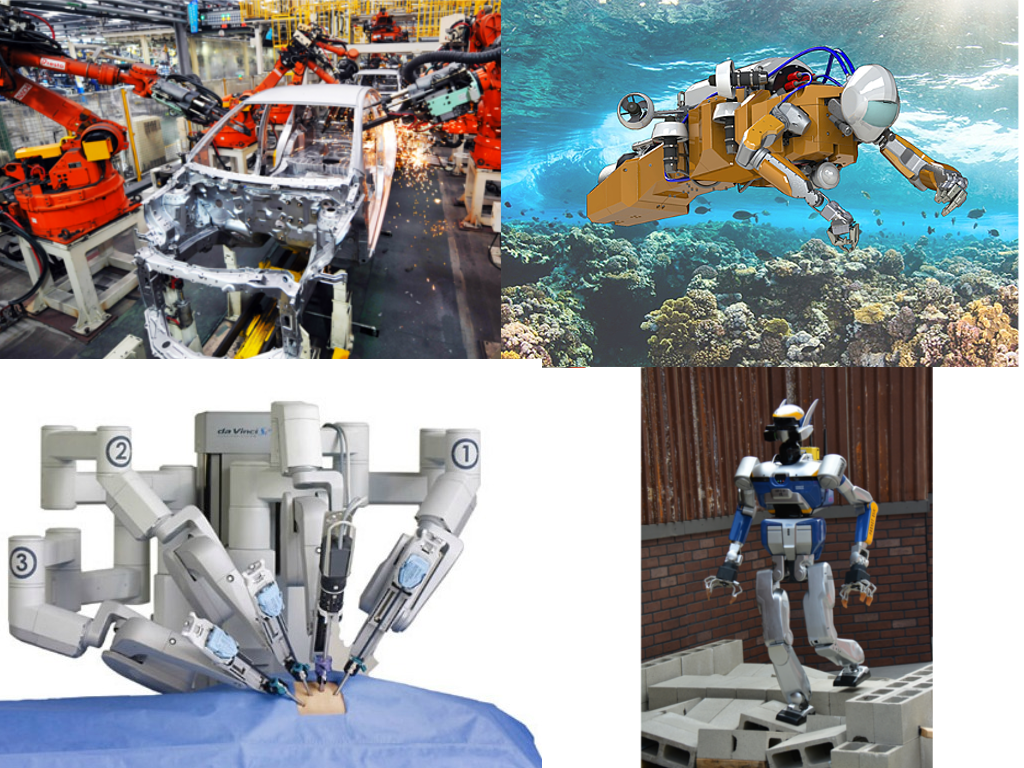
\includegraphics[width=0.9\textwidth]{various-tasks.png}
  \caption{Various robots doing various tasks}
\label{fig:various}
\end{figure}

The DARPA Robotics Challenge has shone some light on the humanoid robots.
This competition brought together a large scope of robotics groups from universities, laboratories and private companies around a common goal: teleoperate a robot to make it succeed in several challenges without any human physical intervention.
The robots were expected to drive a car, open a door, climb stairs, cross debris, drill a hole in a wall, etc.
All those tasks can usually be broken down into sets of elementary tasks in human language.
Some typical examples of tasks for a robot can be `Put hand in contact with target', `Put foot on next step', `Avoid collision with that object', `Maintain stability' or `Look in that direction'.
As is, those tasks do not mean anything for the robot.
A robot is made of a collection of bodies that are linked together by joints actuated by motors.
A robots configuration consists of the position and orientation of its base body, and the configuration of each of its joints.
Satisfying a task requires that the joints of the robot reach a configuration for which the task is satisfied.
The action of satisfying a task comes down to moving from an initial configuration to a goal.
Computing the trajectory to follow and actually following it are the jobs of the trajectory generation and the control of the robot.
Those are by themselves some complete fields of robotics, and they have one thing in common, they both need to be given an initial and a final configuration, and sometimes some intermediate ones.
Finding those configurations is the job of what we call the Posture Generator (PG).

There are two types of robots. The fixed-base robots and the mobile ones.
The first type of robots have fixed basis, the area that they can reach is predefined by their geometry and they are usually fully actuated.
This means that the robot has as many degrees of freedom (DoF) as actuators, Thus, for any joint configuration, a unique robots position can be achieved.
On the contrary, mobile robots are always underactuated, the robot has more DoF than actuators.
Each link of the robot is actuated, but the position of the basis of the robot depends on the configuration of the joints as a well as on the locations of the contacts that the robot makes with the environment.

%A mobile robot's position depends on the location of its contacts with the environment.
%For biped robots evolving on a flat surface, a footstep planner can be used to decide of the sequence of steps to take so the robot can walk to its goal.

Humanoid robots are expected to move and achieve tasks in ways similar to humans.
On flat surfaces, they can walk based on a cyclic motion and the locations of footsteps can be generated by a footstep planner using some simplified models to maintain the robots stability.
In cumbersome and unstructured environments, we humans move in a non-gaited acyclic way: we choose appropriate parts of our body to create contacts with the surrounding environment in order to support the motion of the remaining parts while avoiding obstacles.
A whole motion is a sequence of contact creations and releases.

Since we are biped, we mostly use our feet to move.
As the environment becomes more difficult to cross, hands may come into play together with feet to help with the motion.
Narrow passages may even require other parts of our body (knees, elbows, back\dots) to make contact in order to support the motion.

Planning the sequence of contacts to achieve is a necessary step in devising a motion for a robot.
Once the key stances of the motion have been identified by the planner, they can be used by the controller or the trajectory planner and finally the motion can be achieved by the robot.

All the aforementioned planning methods rely on the fact that we have a tool to decide if a proposed set of contacts is feasible or not for the robot.
The tool used for finding a robot configuration that satisfies a set of various constraints like the geometric constraints of contact or the stability of the robot is called a `Posture Generator' (PG) and the development of that tool is the main topic of this dissertation.

The mission of a posture generator is, for a polyarticulated system, to find a configuration so that the system satisfies a set of constraints.
For simple systems, with simple constraints, like a 6 DoF robotic arm having to reach a point with its end effector, some closed-form expressions can sometimes be devised.
But computing robot configuration to meet the requirements of a given set of tasks, within a viable state, is a recurrent problem whose complexity grows with that of the robot.
When the robotic problem studied becomes too complex for closed-form formulas, it is formulated as a nonlinear optimization program and solved using optimization algorithms.
The Posture Generator is a key tool of many robotics applications and as such, it is an important component of any robotics framework.
It needs to be efficient at finding a solution when one exists and at figuring when a problem is not feasible.
The speed of generating a multi-contact sequence is directly related to the quality of the posture generator, which is directly related to the quality of the optimization algorithm that it uses.

The variables of a robotics problem sometimes naturally belong to a non-Euclidean manifold $\mathcal{M}$, like $SO(3)$ for the 3D rotation of the base of a mobile robot.
A manifold is a topological space that locally resembles Euclidean space near each point.
Each point of an n-dimensional manifold has a neighbourhood that is homeomorphic to the Euclidean space of dimension n.
An n-dimensional non-Euclidean manifold cannot always be globally parameterized over a subset of $\mathbb{R}^n$ without presenting problems of singularity.
Most of the optimization solvers available make the assumption that the search space is Euclidean and thus, do not feature the capability of solving problems on non-Euclidean manifolds natively.
But it is often possible to parametrize $\mathcal{M}$ over a higher dimensionality Euclidean space with added constraint (e.g. unit quaternions, rotation matrices).
It is then possible to solve those problems with classical solvers at the cost of additional variables, constraints and special treatments in the optimization problem.
There exists some methods and algorithms to solve optimization problems on non-Euclidean manifolds with no substantial extra cost and guaranteeing a good coverage of the manifolds without facing parameterization singularities and with the minimal number of parameters, though to our knowledge, they are focused on non-constrained optimization.

%Usually, the solver used for solving optimization problems is a black box on which the user has a very limited control.
During this thesis, we develop our own nonlinear constrained optimization solver on manifolds, that we use to solve optimization problems on their native search manifolds, should they be posture generation problems or others.
This has the added advantage that unlike off-the-shelf solver, which are often a black box on which the user has a very limited level of control, we have full control over that solver and can specialize/modify it to fit our needs.

%\paragraph{Specificities of our approach}
%If we consider a problem of posture generation on a mobile robot with $n$ joints, the configuration space of the joints of the robot is $\mathbb{R}^n$ and the configuration space of the position and orientation of its base body is $SE(3) = \mathbb{R}^3\times SO(3)$.
%Thus, the variable that describes the configuration of the robot in the optimization problem lives in $\mathbb{R}^3\times SO(3) \times \mathbb{R}^n$.
%$SO(3)$ is by nature a non-Euclidean manifold, it cannot be parameterized on an open subset of Euclidean space without having to deal with problems of gimbal lock.
%The gimbal lock is a singularity that happens when parameterizing $SO(3)$ on $\mathbb{R}^3$, with Euler angles, for example, and when two axis of rotation become aligned, in that situation, 2 elements of the parameterization correspond to the same rotation.
%Thus, one degree of freedom is lost.
%Note that this singularity can block the optimization algorithm and that it is only due to the choice of parameterization, it is not intrinsic to the manifold $SO(3)$.
%It is possible to parameterize $SO(3)$ without having to face singularities by parameterizing it over another non-Euclidean manifold.
%The most common ones are the unit quaternion space and the $3\times 3$ rotation matrix.
%Most of the solvers available make the assumption that the search space is Euclidean, which makes is complicated to use quaternion or rotation matrix efficiently.
%To put it simply, for the unit quaternion parameterization, a variable on $SO(3)$ is represented by 4 parameters, the coefficients of the quaternion and an equality constraint needs to be added to the optimization problem to ensure that the quaternion is of norm 1, $\{q\in\mathbb{R}^4:||q||=1\}$.
%Similarly, if a variable is parameterized by a rotation matrix, then the variable $M$ has 9 parameters and several constraints need to be added to the problem so that M is symmetric, positive definite and its determinant is 1 $\{M\in\mathbb{R}^{3\times 3}:M^T M = \mathbb{I}_3\  \&\ \det (M) = 1\}$.
%Similar issues can be found with the parameterization of other non-Euclidean manifold, like $S2$ for example.

%There exists some methods and algorithms to solve optimization problems on non-Euclidean manifolds with no substantial extra cost and guaranteeing a good coverage of the manifolds without facing parameterization singularities and with the minimal number of parameters, though to our knowledge, they are focused on non-constrained optimization.

\paragraph{Contributions and plan}
The main focus of this thesis is the formulation and resolution of problems of posture generation for robotics systems using nonlinear optimization on manifolds.
Our contributions are of two types, on one hand we propose some extensions and improvements on the way to formulate a posture generation problem, and on the other hand, we investigate new ways of solving those problems.
The organization of this thesis is as follows:
%In Chapters~\ref{cha:state_of_the_art} and~\ref{cha:posture_generation_problem_formulation}, we present the background of posture generation, with respectively a state of the art and a presentation of the detailed formulation of a posture generation problem.
%We present several
\begin{itemize}
  \item In Chapter~\ref{cha:state_of_the_art_and_problem_definition} we give the state of the art of posture generation and optimization on manifolds.
  \item In Chapter~\ref{cha:posture_generation_problem_formulation}, we present the detailed formulation of a posture generation problem.
  \item In Chapter~\ref{cha:extensions_of_posture_generation} we present three different and unrelated contributions: two formulation extensions, one allowing to generate non-inclusive contacts between convex surfaces, the other is the exact derivation of the torques in the actuators of a robot.
  Then we present our endeavor to use the `Lifted Newton Method' to solve posture generation problems.
  \item Chapter~\ref{chapter:optimization_on_noneuclidean_manifolds} describes the principles of nonlinear optimization over non-Euclidean manifolds and our implementation of a solver based on those principles.
  \item In Chapter~\ref{ch:PG}, we present a framework that simplifies and extends the formulation of posture generation problems by formulating and solving the optimization problem over native non-Euclidean manifolds, managing automatically the variables of the problems and proposing a framework that formalizes and simplifies the writing of functions on geometric entities often used in robotics.
  \item In Chapter~\ref{cha:evaluation_and_experimentation}, we evaluate the performances of our solver on manifolds and of our posture generator, and then present a preliminary work on how to generate postures on a sensory acquired environment.
\end{itemize}




\chapter{State of the art and Problem definition}
\label{cha:state_of_the_art_and_problem_definition}

\graphicspath{{Chapter1-State-of-the-art/Figs/}}

\section{State of the art}
\label{sec:state_of_the_art}

\subsection{Inverse Kinematics}
\label{sub:inverse_kinematics}

Posture generation can be viewed as, and is sometimes called, Generalized Inverse Kinematics.
The Inverse Kinematics(IK) problem consists in finding the joint configuration for an articulated multibody to complete a given set of tasks in order to generate believable motions.
By definition, it is purely kinematics, and has no regards for stability, or other physics related constraints.
The IK problem has been widely studied and used in the fields of robotics, computer graphics, computer games and animation.
In some cases, for example with robotic arms that have less than 7 degrees of freedom, a closed-form solution can be found, in ~\cite{asfour2003human} the redundancy in a robot arm is exploited to devise a closed-form formula for its IK.
But for more complicated cases, optimization methods are usually used.


%Generating desired initial, intermediary or finale posture configurations requires defining static task goals (e.g.\ reach a target point in 6D) to be done under intrinsic constraints such as joint limits, torque limits, avoiding non-desired self-collisions\ldots and perceptual or extrinsic ones such as keeping an object in the embedded camera field-of-view, avoiding non-desired collisions with surrounding objects, etc.

Many approaches to solve IK problems use pseudo-inverse or Gauss-Newton based methods that are the Jacobian inverse and its variations, Jacobian transpose, damped least squares with and without singular values decomposition or selectively damped least squares~\cite{balestrino1984robust, tolani2000real, baillieul1985kinematic, wampler1986manipulator, nakamura1986inverse, buss2005selectively}.
Those approaches are all computationally expensive and suffer from singularities~\cite{aristidou2009inverse}.

In~\cite{pechev2008inverse} an alternative method based on a control approach is proposed, where no matrix manipulation is required, this approach is as fast as the damped least squares, but outperforms them in terms of handling singularities.
The closed-loop inverse kinematics scheme presented in~\cite{siciliano1990closed} is a famous approach to solve IK problems in a control context.
It uses a second order tracking scheme to guarantee satisfactory tracking performances.

Handling conflicting constraints in IK is a challenging problem to which \cite{baerlocher2004inverse} and \cite{sentis2005synthesis} propose solutions by enforcing a number of priority levels among constraints in their resolution schemes to generate whole-body control of complex articulated figures.

Some statistical resolution approaches have been proposed in~\cite{courty2008inverse, hecker2008real}, with respectively a sequential Monte Carlo method and a particle filtering approach, they have the advantage to only use direct calculations and never require matrix inversions, thus, their strength shows particularly when solving problems with high numbers of degrees of freedom.

In~\cite{AristidouFABRIK, Aristidou:2016_ExtFABRIK} the forward and backward reaching inverse kinematics(FABRIK) resolution method is introduced.
It is based on a geometric iterative heuristic approach, where the bodies of a robot are moved iteratively and separately to reach a target with the end effector while maintaining the integrity of the robot's structure.
This approach is simple, does not suffer from singularities and requires less iterations than most other IK methods.
But it cannot easily be extended to take non-geometric constraints into account.

Finding a solution to an IK problem without regards for the stability of the solution is a common approach in the field of randomized path planning.
\cite{cortes2002random} proposes a method to generate many random configurations for closed loop systems with an increased probability that they be kinematically valid in terms of closure constraints, these configurations are then used in the construction of a Probabilistic RoadMap. In~\cite{lavalle1999probabilistic}, a similar approach is presented where instead of increasing its probability of validation, the closure constraint is enforced for each configuration by additional treatment.

\subsection{Generalized Inverse Kinematics}
\label{sub:generalized_inverse_kinematics}

The Generalized Inverse Kinematics refers to a problem similar to the Inverse Kinematics in the sense that it searches a joint configuration for an articulated figure to complete a task, but needs to do so while respecting other constraints, like ensuring the stability of the structure, respecting its torque limits, avoiding collision with the environment or with itself, etc.

All the previously mentioned approaches are used to find a robot configuration solution to the geometric IK problem.
To solve a Generalized Inverse Kinematics problem with stability constraints, one can first solve the associated IK with one of the methods presented above, and then test the stability of the IK solution, using methods such as the ones presented in~\cite{bretl:itro:2008} or~\cite{rimon2008general} that determine if the configuration can be statically stable.
This gives a rejection criterion for the proposed solution.
If the solution can be stable, the optimal contact forces can be computed using method proposed in~\cite{boyd2007fast} (which in turn allow to compute the joint torques).
Otherwise, another IK solution is generated and tested.
And the process is repeated until a satisfactory solution is found.
This type of sequential approach of posture generation problem resolution features a rejection criterion that can in some cases be difficult to overcome, making this approach costly, for example, if there is a small number of contacts and very few configurations are stable.

%Those approach lead to a sequential resolution of the posture generation problem where a solution to the IK problem is searched, then tested for stability, if it is stable, the optimal forces are computed, otherwise, another solution is searched for.

Another way to solve the posture generation problem is to consider the complete problem as one, with the IK targets and all the other constraints (stability, collisions, torque limits, etc.) in a single nonlinear constrained optimization problem.
In~\cite{Zhao1994}, Zhao uses that approach to solve the IK problem.
That is the approach that we and many others use to solve Generalized Inverse Kinematics problems.
In~\cite{escande:iros:2006}, that approach is employed to generate postures that are used to grow a tree of usable postures in a multi-contact planning algorithm.
It was applied to automatically generate a sequence of contact sets and postures where the HRP-2 robot uses its hand to lean on a table in order to grasp an object otherwise out of reach.
Interestingly enough, in that study, the C-code that computes the robot's kinematics is generated through Maple and the HuMAnS toolbox~\cite{wieber2006humans} provided by INRIA.
The constraints of contact, stability and collision are then computed on top of it.
And the problem is solved by the CFSQP solver~\cite{cfsqp:manual}.
In~\cite{hauser:ijrr:2008}, a similar posture generation approach is used to find viable postures for different legged robots on varied terrains in the context of a Probabilistic RoadMap planning, which is a planning approach based on random sampling of the configuration space.
%\cite{hauser:issr:2007} presents a different approach to multi-contact planning based on probabilistic roadmap and random sampling of the configuration space.
In~\cite{bouyarmane2010static}, Bouyarmane proposes a generalization of the formulation of posture generation problems for systems of multiple robots and manipulated objects.
Also, he generalizes the notion of contacts by allowing them to bear contact forces or not and to not necessarily be coplanar or horizontal.
This generic formulation enables the generation of postures with inter-robot contacts.
The complete posture generation problem is then solved within a single nonlinear constrained optimization query, computing the contact forces and joint configuration at the same time, while ensuring the stability of all the actors, avoiding collision and respecting the robot's joint and torque limits.

In the past few years, our team has dedicated considerable efforts in proposing a general multi-contact motion planner to solve cases of non-gaited acyclic planning, using a posture generator as a backbone to select valid configurations.
Given a humanoid robot, an environment, a start and a final desired postures, the planner generates a sequence of contact stances allowing any part of the humanoid to make contact with any part of the environment to achieve motion towards the goal.
The planner's role is to grow a tree of contact stances iteratively; from a given posture, it tries to add of remove contacts one by one.
The tree grows, following some heuristics until the solution is reached.
For each set of contacts to add to the tree, a posture generation problem is solved in order to validate the feasibility of the set, if it is not feasible, the set is rejected.
A typical experiment with a HRP-2 robot achieving such an acyclic motion is presented in~\cite{escande:iser:2008}, and the planner is thoroughly described in~\cite{escande:ras:2013}.
Extensions of this multi-contact planner to multi-agent robots and objects gathering locomotion and manipulation are presented in~\cite{bouyarmane:ar:2012}, and preliminary validations with some DARPA challenge scenarios, such as climbing a ladder, ingress/egress a utility car or crossing through a relatively constrained pathway are presented in~\cite{bouyarmane:humanoids:2012}.
Another way of planning a multi-contact scenario, which is actually often used when planners fail to find satisfactory solutions, is to do it manually, choosing iteratively which contacts to add and remove until the goal is reached.
This type of approach is used when the plan to execute is complex and when a lot of fine tuning of the postures is required, as in~\cite{vaillant:autonomousrobots:2016}, where a sequence of postures allowing the HRP-2 robot to climb a vertical ladder is generated and tuned manually.
Those postures are provided as input to a finite state machine that builds additional intermediary tasks and specific grasps procedures to be realized on the real robot by a multi-objective model-based QP controller.
Instead of feeding the key postures directly to the controller and trusting that it will find a path to connect them, one can take an additional step and compute a dynamically viable trajectory between successive steps that the controller will then have to follow as presented in~\cite{lengagne2013generation}.
That allows to take advantage of the dynamic effects and produce motions with better performances in terms of completion time, energy consumption, or other criterions.
Although the key postures are guaranteed to be viable by the posture generator, the whole trajectory might not be.
Interval analysis methods can be leveraged to ensure the satisfaction of constraints over the whole duration of a motion, as proposed in~\cite{lengagne2011planning}.

In many planning approaches~\cite{kuffner2005motion, chestnutt2007navigation, hauser:ijrr:2008, kolter2008control, bouyarmane:icra:2011} the planning problem is decomposed in two stages, first the sets of contacts and associated postures are planned and then the motions to go from one set to another are computed.
Those two stages are loosely coupled, which can result in suboptimal use of the contacts available.
\cite{mordatch:acm:2012} presents a different approach to contact planning where some additional terms and variables are added to the optimization problem to decide whether a contact pair should be active(and bear forces) at any given time during the motion.
The contact sets, as well as the postures associated are discovered along with the entire movement's trajectories by using contact invariant optimization.
This allows to exploit any synergies that might exist between the contact events and the motion trajectory.

In~\cite{liu:acm:2012}, posture generation is used to find the optimal posture and position of contacts to optimally realize a manipulation task along a path, while satisfying geometric and kinematic constraints as well as force and torque constraint.
The task is defined as a path and force to follow with an end effector.
Instead of finding a sequence of unrelated postures along the path, all the postures are found by solving a single optimization problem in which successive postures are coupled by constraints to ensure that the foot positions remain constant during the task, even though the rest of the body can move.
This approach allows the robot or virtual character to apply manipulation forces as strongly as possible while avoiding foot slippage.
It also allows to take external perturbations into account to generate more robust postures.

Another utilization of posture generation was presented in~\cite{stasse:humanoids:2007}, that deals with the problem of object reconstruction.
An object is presented to the robot in order to generate automatically its 3D model.
To do so, the object is observed from several different angles with the camera that is mounted in the robot's head.
The satisfactory postures of the robot to complete this task are obtained by solving a posture generation problem to which a set of constraints defining the direction in which the robot should look and a minimum distance from the object are added.
In that work, the observation directions are predefined,~\cite{foissotte:humanoids:2008} presents an approach where the choice of the best observation direction is left to the posture generator.
The representation of the object is iteratively carved into a block of 3D voxels, each new point of view chosen to allow to carve it a little more precisely.
It uses a modified cost function to evaluate the amount of information on the object that a given point of view can provide.
The posture of the robot that optimizes that cost function is then found by the posture generator under the classical constraints of stability, collision avoidance and other robot's limitations.


\subsection{Optimization}
\label{sub:optimization}

The resolution of a posture generation problems is often done by solving a nonlinear optimization problem which consists in finding the optimal point that minimizes a cost function, possibly subject to constraints, the cost and constraints functions being possibly nonlinear.

Optimization algorithms can be derivative-free or not.
The computation of the derivatives of the functions involved in the problem is a common source of error.
The strength of the derivative-free approaches is that the user does not need to implement the derivatives.
But those approaches are much slower than their counterparts using derivatives.
One way to avoid implementation errors in the derivatives computation is to use finite differences to compute them.
This method is very slow, especially when the dimension of the problem is large.
In order to design an efficient optimization algorithm, we will focus on methods using derivative informations and will implement those derivatives' computations.
The finite difference approach can be used to verify the correctness of the computed derivative.

Nonlinear optimization is a wide topic that has been extensively studied in the past.
One can find some excellent reference books about it, such as~\cite{nocedal:book:2006, bonnans:book:2003, boyd2004convex}.

Furthermore, several off-the-shelf solvers are available and have been widely used in for solving robotics problems.
The CFSQP solver~\cite{cfsqp:manual} was used in~\cite{escande:iros:2009} and~\cite{escande:ras:2013} where thousands of HRP-2 posture generation queries were made to explore the feasible space.
The IPOPT solver~\cite{wachter:mathprog:2006} has been used in~\cite{vaillant:humanoids:2014},~\cite{vaillant:autonomousrobots:2016},~\cite{bouyarmane:ar:2012} where the posture generator had been extended to handle multi-robot problems and more complex and various contact models.
The SNOPT solver~\cite{gill2005snopt} was used in~\cite{dai2014whole} to plan dynamic whole-body trajectories.
Several nonlinear optimization solvers are available and have been packaged for use in robotics problems in the Roboptim Framework~\cite{moulard:jsme:2013}, such as IPOPT, CFSQP, CMinPack~\cite{cminpack}, NAG~\cite{nag}, KNITRO~\cite{knitro} and PGSolver(the solver that we develop in this thesis).

Traditionally, optimization problems are solved over Euclidean spaces.
When the need comes to find a solution to an optimization problem in a non-Euclidean space $\mathcal{M}$, the commonly used method is to represent the elements of $\mathcal{M}$ in a Euclidean manifold of higher dimension, and enforcing that solution of the optimization problem should lie on $\mathcal{M}$ by adding the necessary constraints to the problem.
We will detail the drawbacks of such approaches in Chapter~\ref{chapter:optimization_on_noneuclidean_manifolds}.
Alternatively, there exist some method to run an optimization algorithm directly on a non-Euclidean manifold, as it is presented in great details in the book~\cite{absil:book:2008}.
A non-Euclidean manifold, can be thought of as a space that is locally Euclidean, but not globally.
For example a sphere, if one looks in a small enough neighborhood, looks Euclidean, just like the surface of a giant sphere like the earth looks flat for a human being standing on it.
Based on the fact that manifolds are locally Euclidean, the classic properties of distance, derivatives, and in general all the Euclidean geometry can be used locally.
Based on that property, several optimization methods traditionally used on Euclidean manifolds have been extended to manifolds.
The gradient methods have been extended to manifolds in~\cite{luenberger1972gradient, gabay1982minimizing}.
The Newton methods on manifolds which have better convergence rates were extended to manifolds in~\cite{gabay1982minimizing, stuart1998dynamical, smith2013geometric}.
And Quasi-Newton methods in~\cite{gabay1982minimizing}.
Those approaches are only meant to solve unconstrained optimization problems, which is not enough to solve posture generation problems, where the presence of constraints in unavoidable.

The main idea to optimize on manifold is that we use a local map between the neighborhood of the current iterate and its Euclidean tangent space in order to run an optimization step and choose an increment in the tangent space that is mapped back to the manifold.
Once the iterate has been incremented, the process is repeated with the map and tangent space associated with the new iterate.
This comes down to re-parameterizing the problem around the current iterate at each iteration.

In the field of robotics, we are only aware of the work of Schulman \emph{et al.}~\cite{Schulman2014}, where the authors explain the adaptation of their solver to work on $SE(3)$.
In the field of computer vision, and especially for solving pose estimation problems, optimization on manifolds is often used, e.g.~\cite{hertzberg2011, lu2000fast}.

In this thesis, we develop a nonlinear solver on manifolds that can handle constraints, and were largely inspired by the work of Fletcher concerning the notions of Sequential Quadratic Programming without a penalty method~\cite{Fletcher:ifip:2006, fletcher2010sequential, fletcher:mathprog:2000}, along with other optimization approaches that we adapted to work with manifolds.

\section{Problem Definition}
\label{sec:problem_definition}

%%%%%%%%%%%%%%%%%%%%%%%%%%%%%%%%%%%%%%%%%%%%%%%%%%%%%%%%%%%%%%%%%%%%%%%
%                     SECTION PROBLEM DEFINITION                      %
%%%%%%%%%%%%%%%%%%%%%%%%%%%%%%%%%%%%%%%%%%%%%%%%%%%%%%%%%%%%%%%%%%%%%%%

We consider the problem where we have a robotic system and we want it to realize a set of tasks $T_i$.
We denote $\bf q$ the joint configuration ($n$ joints + base) of the robot, and $\mathbf{f} =\{\mathbf{f}_i\,, i\in[1,m]\}$ represents the $m$ contact forces applied on the robot.
Each task $T_i$ can be represented by a set of equality and inequality equations:
\begin{equation}
  \left\{
    \begin{aligned}
    g_i(\mathbf{q},\mathbf{f}) = 0\\
    h_i(\mathbf{q},\mathbf{f}) \geq 0
    \end{aligned}
  \right.
\end{equation}
For example, the task of making contact between a body of the robot and a part of the environment can be represented in such a way.

In addition to satisfying the tasks $T_i$, the solution configuration to our problem must describe a viable posture of the robotic system, in the sense that it ensures its integrity.
Which translates into the following list of constraints.
It must respect the joint limits of the robot~\eqref{subeq:bounds}, as well as its torque limits~\eqref{subeq:tau}.
Equation~\eqref{subeq:autocoll} translates the auto-collision avoidance constraint between a pair of bodies $\{r_i, r_j\}$ given by $\mathcal{I}_\text{auto}$ where $d$ is the minimal distance between two bodies.
Equation~\eqref{subeq:coll} denotes the collision avoidance constraint between a robot body $r_i$ and an object of the environment $O_k$ defined in $\mathcal{I}_\text{coll}$.
$\epsilon_{ij}$ and $\epsilon_{ik}$ denote the minimal acceptable distance for their respective constraints.
The stability of the robot is ensured by the respect of equation~\eqref{subeq:stab}, which is the Euler-Newton equation(or a simplification of it).
To avoid slippage of the contacts, the contact force must remain in the Coulomb friction cone, which is enforced by equation~\eqref{subeq:friction}.
Equations~\eqref{subeq:gi} and~\eqref{subeq:hi} translate the constraints to satisfy task $T_i$.

The set of satisfying configurations can be defined by $\mathcal{Q}$:

\begin{empheq}[left={\mathcal{Q}=\{\mathbf{q}, \mathbf{f}\}:\empheqlbrace}]{align}
      & q_i^- \leq q_i \leq q_i^+ \quad \forall i\in[1,n] & \text{joint limits} \label{subeq:bounds}\\
      & \tau_i^- \leq \tau_i(\mathbf{q}, \mathbf{f}) \leq \tau_i^+ \quad \forall i\in[1,n] & \text{torque limits}\label{subeq:tau}\\
      & \epsilon_{ij} \leq d(r_i(\mathbf{q}), r_j(\mathbf{q})),\quad \forall (i,j)\in\mathcal{I}_\text{auto} & \text{auto-collision}\label{subeq:autocoll}\\
      & \epsilon_{ik} \leq d(r_i(\mathbf{q}), O_k),\quad \forall (i,k)\in\mathcal{I}_\text{coll} & \text{collision}\label{subeq:coll}\\
      & s(\mathbf{q}, \mathbf{f}) = 0 & \text{stability} \label{subeq:stab}\\
      & c(\mathbf{f}_i) \geq 0 \quad i\in[1,m] & \text{slippage avoidance} \label{subeq:friction}\\
      & g_i(\mathbf{q}, \mathbf{f}) = 0 & \text{task i's equalities}\label{subeq:gi}\\
      & h_i(\mathbf{q}, \mathbf{f}) \geq 0 & \text{task i's inequalities} \label{subeq:hi}
\end{empheq}

We illustrate those constraints in figure~\ref{fig:PG} and will explicit them in more details in Chapter~\ref{cha:posture_generation_problem_formulation}.

%Where inequalities~\eqref{subeq:bounds} represent the joint limits, and~\eqref{subeq:tau} the torque limits.

\begin{figure}[ht]
  \centering
  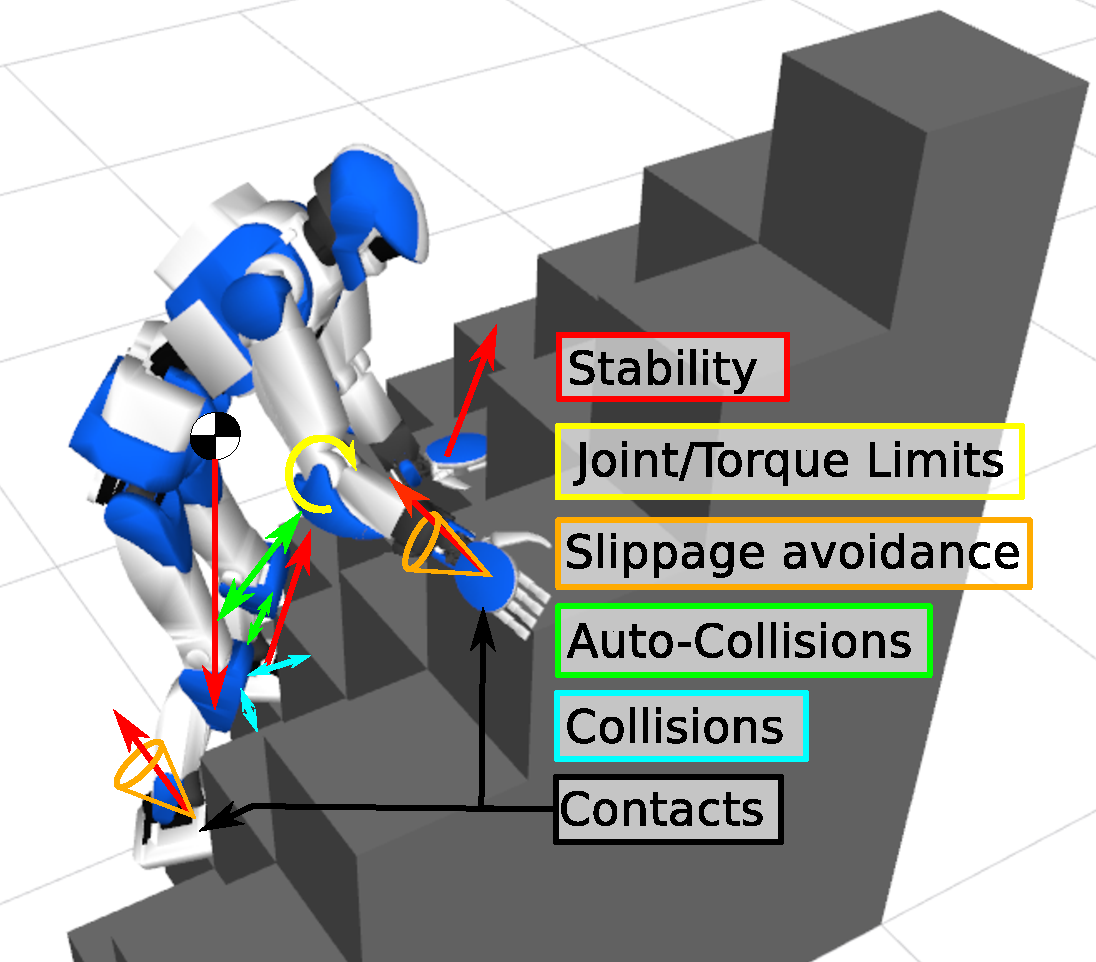
\includegraphics[width=0.7\textwidth]{PG.pdf}
  \caption{HRP4 on a stack of cubes. The color of each box corresponds to the color of the constraint it depicts.}
\label{fig:PG}
\end{figure}

In addition to satisfying the set of constraints $T_i$ while being viable, one can require the searched posture to be optimal in the sense of some cost function $f$.
Defining a cost function can help the user control the result of the problem, by for example minimizing the distance to a reference posture or maximizing the contact force applied by one end-effector.
In~\cite{escande2009} the cost function was used to guide the posture toward the end of a planning problem.
A sum of different criterions can be used as cost function.
The optimization problem that describes the posture generation problem becomes:


%We consider the problem where we have a robotic system and we want it to do some tasks, like for example to make a contact between a point on a body of the robot and a point of the environment.
%This contact task can be modelized as a simple equality.
%We denote $q$ the joint configuration (joint + base) of the robot, $g(q)$ is the 3D position of the point of interest on the robot and $P$ is the point of the environment.
%Then our problem comes down to finding a configuration $q^*$ such that $g(q^*) = P$.
%For robots like humanoids, the equations describing their kinematics are quite complicated, and, in the presence of angular joints, they are nonlinear.
%In the general case, even for simple tasks, a closed form solution of the problem does not exist.

%We denote $\mathcal{C}$ the configuration space of our robotic system.
%It is the manifold in which $q$ lives. The dimension of $\mathcal{C}$ is equal to the number of degrees of freedom of the robot.
%Note that if all the joints of the robot are actuated, this is the number of motors of the robot.
%And if the robot has a free-floating basis (is not fixed) then the position in $\mathbb{R}^3$ and rotation in $SO(3)$ of its basis are part of $q$.

%We can formulate that problem as follows:

%\begin{equation}
  %\text{find}\ q\in\mathcal{C}\ \text{such that}\ g(q)=P
%\end{equation}

%The space of solution of this problem is a submanifold of $\mathcal{C}$ that we call ${\mathcal{C}}_F$ the feasible configuration space (which can be empty).

%In addition to the equality constraint abovementioned, the problem can feature some inequality constraints.
%For example, each joint variable can be limited to a certain range of value: $\forall i,\ q_i\in [q_i^-,\ q_i^+]$.
%Then the problem becomes a combination of equality and inequality constraints.%, and can be written as:
%%\begin{equation}
  %%\text{find}\ q\in\mathcal{C}\ \text{such that}\left\{
  %%\begin{array}{l}
    %%g(q)=P \\
    %%\forall i,\ q_i^- \leq q_i \leq q_i^+
  %%\end{array}
  %%\right.
%%\end{equation}
%Finally, we can also require finding the point of $\mathcal{C}_F$ that minimizes a criterion, such as the distance to a goal posture $q_0$.
%Our problem becomes:

%\begin{equation}
  %\left\{
  %\begin{array}{l}
    %\minimize\limits_{q\in\mathcal{C}}{\|q-q_0\|_2}\\
    %\text{ s.t. }
    %\left\{
    %\begin{array}{l}
      %g(q)=P\\
      %\forall i,\ q_i^- \leq q_i \leq q_i^+
    %\end{array}
    %\right.
  %\end{array}
  %\right.
%\end{equation}

\begin{equation}
  \begin{array}{l}
    \minimize\limits_{\mathbf{q}, \mathbf{f}}{f(\mathbf{q}, \mathbf{f})}\\
    \text{ s.t. }\{\mathbf{q}, \mathbf{f}\}\in\mathcal{Q}
  \end{array}
\end{equation}

This type of problem is called a nonlinear constrained optimization problem and can be formulated in a more generic fashion as:

\begin{equation}
\label{eq:optim_form_PG}
  \begin{array}{l}
    \minimize\limits_{x}{f(x)}\\
    \text{ s.t. }
    \left\{
    \begin{array}{l}
      c_i(x) = 0,\ \forall i\in{E}\\
      c_i(x) \geq 0,\ \forall i\in{I}\\
    \end{array}
    \right.
  \end{array}
\end{equation}

Where $x$ is the optimization variable we want to find that minimizes the cost function $f(x)$ while satisfying the equality constraints $c_i(x) = 0,\ \forall i\in{E}$ and inequality constraints $c_i(x) \geq 0,\ \forall i\in{I}$.
Such problems can be solved by a nonlinear optimization solver.
In Appendix~\ref{chapter:optimization}, we present some principles of nonlinear optimization in unconstrained and constrained cases.
%Several off-the-shelf solvers are available and have been widely used in for solving robotics problems.
%The CFSQP solver~\cite{cfsqp:manual} was used in~\cite{escande:iros:2009} and~\cite{escande:ras:2013} where thousands of HRP-2 posture generation queries were made to explore the feasible space.
%The IPOPT solver~\cite{wachter:mathprog:2006} has been used in~\cite{vaillant:humanoids:2014},~\cite{vaillant:autonomousrobots:2016},~\cite{bouyarmane:ar:2012} where the posture generator had been extended to handle multi-robot problems and more complex and various contact models.
%The SNOPT solver~\cite{gill2005snopt} was used in~\cite{dai2014whole} to plan dynamic whole-body trajectories.
%Several nonlinear optimization solvers are available and have been packaged for use in robotics problems in the Roboptim Framework~\cite{moulard:jsme:2013}, such as IPOPT, CFSQP, CMinPack~\cite{cminpack}, NAG~\cite{nag}, KNITRO~\cite{knitro} and PGSolver, the solver that we develop in this thesis.

In this thesis, we use the off-the-shelf solvers IPOPT~\cite{wachter:mathprog:2006} in the beginning and later we tackle the development of our own nonlinear solver and then use it.
From this point forward, we formulate and solve posture generation problems as nonlinear constrained optimization problem.
And in the next chapter, we focus on formulating all the basic functions and algorithms used to describe robotics constraints and cost function in the formalism of nonlinear optimization.


%%%%%%%%%%%%%%%%%%%%%%%%%%%%%%%%%%%%%%%%%%%%%%%%%%%%%%%%%%%%%%%%%%%%%%%
%                            First Chapter                            %
%                         Problem Formulation                         %
%%%%%%%%%%%%%%%%%%%%%%%%%%%%%%%%%%%%%%%%%%%%%%%%%%%%%%%%%%%%%%%%%%%%%%%

\chapter{Posture Generation: Problem Formulation}
\label{cha:posture_generation_problem_formulation}

\nomenclature[z-PG]{PG}{Posture Generation}
\nomenclature[z-IK]{IK}{Inverse Kinematics}
\nomenclature[z-DoF]{DoF}{degrees of freedom}
\nomenclature[z-w.r.t]{w.r.t}{with respect to}
\nomenclature[x-I]{$\mathbb{I}_n$}{Matrix identity of dimension $n$}
\nomenclature[x-w]{$\wedge$}{cross product}
\nomenclature[a-F]{F}{a frame}
\nomenclature[a-W]{W}{the world frame}
\nomenclature[a-w]{w}{a wrench or a force}
\nomenclature[a-f]{f}{a force resultant}
\nomenclature[a-m]{m}{a force moment}


\graphicspath{{Chapter2-PG/Figs/}}

%{{{List of contributions
%\section{List of contributions}

%%%%%%%%%%%%%%%%%%%%%%%%%%%%%%%%%%%%%%%%%%%%%%%%%%%%%%%%%%%%%%%%%%%%%%%%
%%                   SECTION LIST OF CONTRIBUTIONS                     %
%%%%%%%%%%%%%%%%%%%%%%%%%%%%%%%%%%%%%%%%%%%%%%%%%%%%%%%%%%%%%%%%%%%%%%%%

%\begin{itemize}
  %\item Generalities, introduction
  %\item Presentation of the existing methods
  %\item From Inverse Kinematics to Generalized IK/posture Generation/pose estimation (addition of articular limits, forces, stability etc).
  %\item Topology of the parametrization space (Free-flyer, q, f, other)
  %\item Formulation as a nonlinear constrained optimization problem
  %\item Adrien \& Karim's formulations
  %\item Formulation of several types of cost/constraints
  %\begin{itemize}
    %\item Contact with planar surface
    %\item Collision avoidance
    %\item Auto-Collision avoidance
    %\item Static equilibrium: Newton/CoM projection
    %\item Forces in friction cones
    %\item Articular limits
    %\item Torque limits
    %\item Torque minimization
    %\item Goal Posture
  %\end{itemize}
  %\item Reasons why it is not enough and why we needed a new PG
    %\begin{itemize}
      %\item Having an easier way to formulate problems
      %\item Avoid having to de some gymnastic to remain on manifolds
      %\item Automatic variable management
      %\item Robustness
    %\end{itemize}
  %\item Utilization of posture generation in planning
%\end{itemize}
%}}}


In this Chapter, we present in detail the formulation of a posture generation problem.
We present the algorithms used to compute the kinematics of a robot and its derivatives as well as the joint torques.
Then we formulate some classical functions that are often used in posture generation: joint limits, contact constraints, collision avoidance, stability, torque limits and friction cones.
In Figure~\ref{fig:PG}, we illustrate those constraints with the result of a posture generation problem where the HRP4 robot must climb on a stack of cubes while being statically stable, respecting its joint and torque limits, the contact forces must remain in the friction cones and the robot must avoid auto-collisions and collisions with the environment.

%\begin{figure}[ht]
  %\centering
  %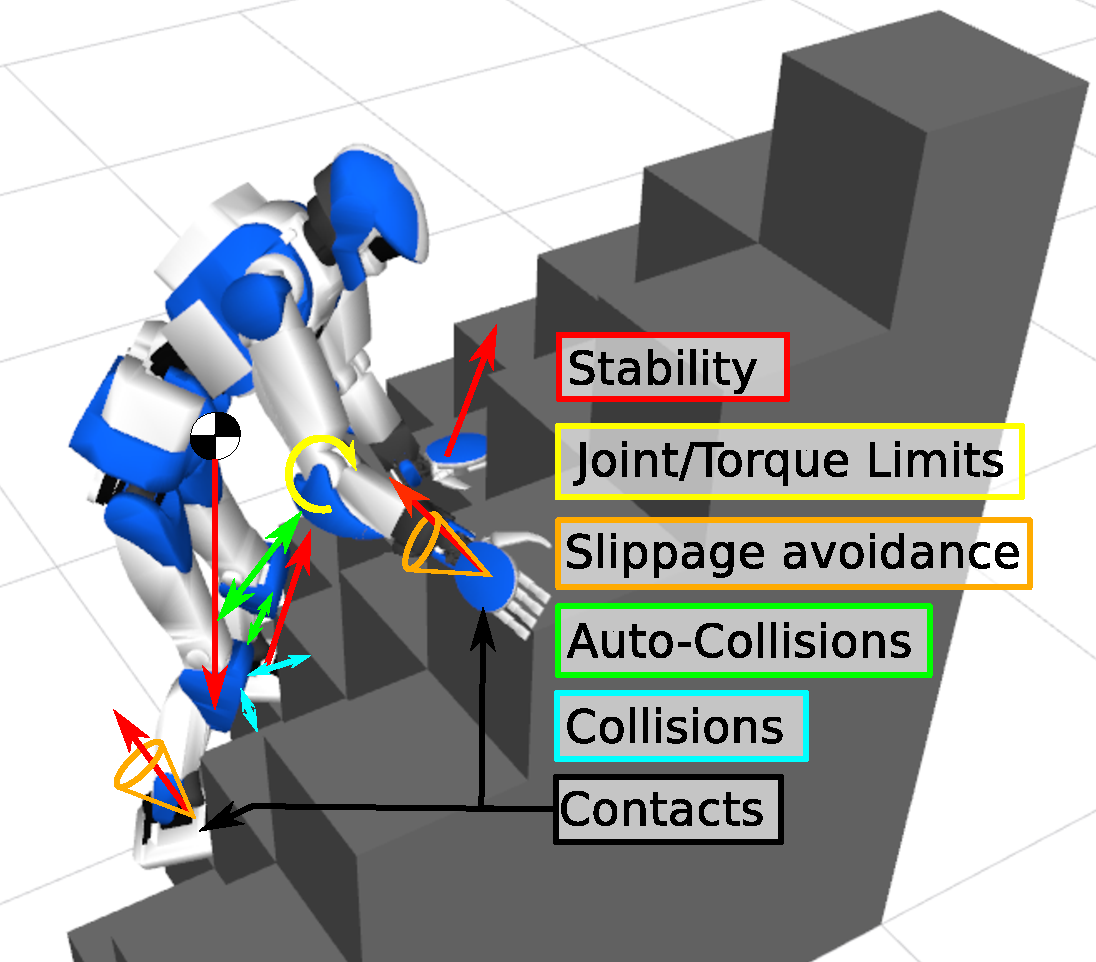
\includegraphics[width=0.7\textwidth]{PG.pdf}
  %\caption{HRP4 on a stack of cubes. The color of each box corresponds to the color of the item it depicts.}
%\label{fig:PG}
%\end{figure}


%%%%%%%%%%%%%%%%%%%%%%%%%%%%%%%%%%%%%%%%%%%%%%%%%%%%%%%%%%%%%%%%%%%%%%%
%                    SECTION PROBLEM FORMULATION                      %
%%%%%%%%%%%%%%%%%%%%%%%%%%%%%%%%%%%%%%%%%%%%%%%%%%%%%%%%%%%%%%%%%%%%%%%
%\section{Kinematics Formulation}
%\label{sec:kinematics_formulation}


\section{Forward Kinematics}
\label{sec:forward_kinematics}

%%%%%%%%%%%%%%%%%%%%%%%%%%%%%%%%%%%%%%%%%%%%%%%%%%%%%%%%%%%%%%%%%%%%%%%
%                   SUBSECTION FORWARD KINEMATICS                     %
%%%%%%%%%%%%%%%%%%%%%%%%%%%%%%%%%%%%%%%%%%%%%%%%%%%%%%%%%%%%%%%%%%%%%%%

In this section, we present a formulation of robotic systems that allows specifying most of the typical constraints encountered in robotics problems.

We consider a robotic system made of $n_B$ bodies and $n_J(=n_B+1)$ joints.
The global structure of the robot is described by an ordered graph called multibody graph.
The base body (World) has index $0$ and other bodies get different positive integer index.
We denote the body of index $i$, $B_i$.
$B_0$ refers to the World.
Each body $B_i$ has its reference frame $F_i$ attached to it.
$F_0$ denotes the World frame.
Bodies are linked together by joints that also are indexed by positive integers, we denote the joint of index $i$, $J_i$, and the body that comes after it is $B_i$.
Each joint defines the relation between its predecessor and successor bodies.
For joint $J_i$, they are respectively denoted $pred(i)$ and $succ(i)$, and $B_{pred(i)}$ is called the parent body of $B_{succ(i)}$.
We denote $\lambda(j)$ the index of the parent body of $B_j$.
The number of degrees of freedom of $J_i$ is denoted $dof^J_i$ and the number of degrees of freedom of the whole robot is denoted $dof$.
Figure~\ref{fig:mbg} illustrates this numbering system for a simple robot with 4 joints and 5 bodies (including the basis)

The geometric relations between bodies and joints are described through transformations between their reference frames.
We use transformations as described in the Spatial Vector Algebra chapter of `Rigid Body Dynamics Algorithm' by Roy Featherstone~\cite{featherstone:book:2007}.
Motion vectors (vectors describing motion quantities as positions, velocities and accelerations) and their force counterpart are defined in~\cite{featherstone:book:2007}.

For any 3D vector $v\in\mathbb{R}^3$, $\hat{v}$ denotes the $3\times 3$ skew-symmetric matrix such that $\hat{v}u = v\wedge u$.
Where $\wedge$ denotes the cross product operator.

Let A and B be Cartesian frames with origins O and P respectively.
Let $\mathbf{t}$ be the coordinate vector expressing $\overrightarrow{OP}$ in A.
And $\mathbf{R}$ be the rotation matrix that transforms 3D vectors from A to B coordinates.
The transformation from A to B for a motion vector is defined by:
\begin{equation}
  {}^B X_A =
  \begin{bmatrix}
    \mathbf{R} & \mathbf{0} \\
    -\mathbf{R}\hat{\mathbf{t}} & \mathbf{R} \\
  \end{bmatrix}
\end{equation}
Its inverse is:
\begin{equation}
  {{}^B X_A}^{-1} = {}^A X_B =
  \begin{bmatrix}
    \mathbf{R}^T & \mathbf{0} \\
    \hat{\mathbf{t}}\mathbf{R}^T & \mathbf{R}^T \\
  \end{bmatrix}
\end{equation}
The transformation from A to B for a force vector is defined by:
\begin{equation}
  {}^B X_A^* =
  \begin{bmatrix}
    \mathbf{R} & -\mathbf{R}\hat{\mathbf{t}} \\
    \mathbf{0} & \mathbf{R} \\
  \end{bmatrix}
\end{equation}
Its inverse is:
\begin{equation}
  {}^B X_A^{-*} = {}^A X_B^* =
  \begin{bmatrix}
    \mathbf{R}^T & \hat{\mathbf{t}}\mathbf{R}^T \\
    \mathbf{0} & \mathbf{R}^T \\
  \end{bmatrix}
\end{equation}

\begin{figure}
  \centering
  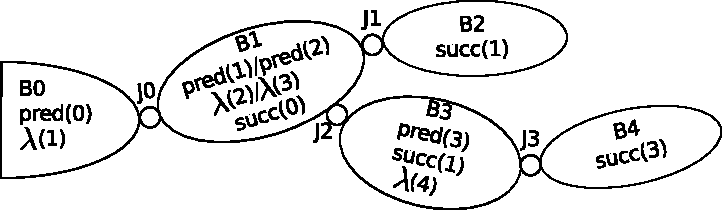
\includegraphics[width=0.7\textwidth]{mbg.pdf}
  \caption{MultiBody graph}
\label{fig:mbg}
\end{figure}

%Each joint $J_i$ is defined in the reference frame of its predecessor body by a static transformation $X^x_i = \{\mathbf{R}^x_i, \mathbf{t}^x_i\}$ from the base of the body to the base of the joint.
Each joint $J_i$ is defined by a static transformation $X^x_i = \{\mathbf{R}^x_i, \mathbf{t}^x_i\}$ between the reference frame of its predecessor body and its own reference frame.
Each joint $J_i$ is associated with a motion subspace which representation matrix is denoted $\mathbf{S}_i$.
Each column of $\mathbf{S}_i$ described a degree of freedom of $J_i$ its upper part for the rotations and lower for translations (see Section~\ref{sec:joints_formulations}).
\begin{equation}
  \mathbf{S}_i =
  \begin{bmatrix}
    S^R_{i,0} & \cdots &
    S^R_{i,j} & \cdots &
    S^R_{i,dof} \\
    S^t_{i,0} & \cdots &
    S^t_{i,j} & \cdots &
    S^t_{i,dof}
  \end{bmatrix}
\end{equation}

For a given joint configuration $q$, the transformation due to the joint $J_i$ current configuration from its reference frame to the reference frame of its successor body is denoted \\$X^J_i (q) = \{\mathbf{R}^J_i (q), \mathbf{t}^J_i (q)\}$.

The transformation between $B_{\lambda(i)}$ and $B_i$ is denoted $X^{PtS}_i (q) = \{\mathbf{R}^{PtS}_i, \mathbf{t}^{PtS}_i\}$ (PtS stands for `Parent to Son') can then be computed as:
\begin{equation}
  {X}^{PtS}_i (q) = {}^{i}X_{\lambda (i)} (q) = X^J_i (q) X^x_i
  \label{eq:PtS}
\end{equation}

Let $\kappa (i) =\{0, i_1, i_2 \ldots i\}$ be the list of indexes of successive joints going from $B_0$ to $B_i$.
It can easily be computed by adding iteratively the parent of the current body:

\begin{algorithm}
  \caption{Joint Path to $B_i$}
\label{alg:JP}
\begin{algorithmic}
  \State{$j \leftarrow i$, $\kappa(i)=[i]$}
  \While{$j \neq 0$}
  \State{$j \leftarrow \lambda(j)$}
  \State{$\kappa(i) \leftarrow [\kappa(i),\ j]$}
  \EndWhile{}
\end{algorithmic}
\end{algorithm}

The transformation from the World base to $B_i$ is denoted \\ ${}^i X_0 (q) = \{{}^i \mathbf{R}_0 (q), {}^i \mathbf{t}_0 (q)\}$.
The formula~\Eqref{eq:PtS} can be used iteratively on all bodies of the robot to obtain the expression of ${}^i X_0 (q)$.

We obtain the full expression of ${}^i X_0$ as:
\begin{equation}
  {}^i X_0 (q) = \prod_{j\in\kappa (i)}X^J_j (q) X^x_j = \prod_{j\in\kappa (i)}\ {}^j X_{\lambda (j)}
  = {}^i X_{\kappa (1)}\ ^{\kappa (1)}X_{\kappa (2)} \dots ^{\kappa (\text{end}-1)}X_{W}
\end{equation}

Which can be computed recursively by a Forward Kinematics algorithm:

\begin{algorithm}
  \caption{Forward Kinematics}
\label{alg:FK}
\begin{algorithmic}
  \For{$i = 0:n_J$}
  \If{$\lambda (i) \neq -1$} ${}^i X_0 = {}^i X_{\lambda (i)}\ ^{\lambda (i)}X_0$
  \Else$\ {}^i X_0 = X^{PtS}_i$
  \EndIf{}
  \EndFor{}
\end{algorithmic}
\end{algorithm}

In the following section, we provide some detailed description of how to compute $X_J (q)$ for a variety of useful joints.
Using the joint descriptions and the Forward Kinematics algorithm, we are able to explicit a relation between $q$ the joint parameters of the robot and the 3D position and orientation of  any geometric quantity defined in the reference frame of a body of the robot.
Given a transformation ${}^p X_i$ defined in the frame of $B_i$, its value in the world frame is given by ${}^p X_0 (q) = {}^p X_i\ {}^i X_0 (q)$



\section{Joints formulations}
\label{sec:joints_formulations}

%%%%%%%%%%%%%%%%%%%%%%%%%%%%%%%%%%%%%%%%%%%%%%%%%%%%%%%%%%%%%%%%%%%%%%%
%                   SUBSECTION JOINTS FORMULATIONS                    %
%%%%%%%%%%%%%%%%%%%%%%%%%%%%%%%%%%%%%%%%%%%%%%%%%%%%%%%%%%%%%%%%%%%%%%%

The entire geometry of our system is described by the list of static transformations $X^x_j$ and of joint transformations $X^J_j (q)$.
In this section, we explicit the descriptions and formulations of several useful joints.

Let us consider a joint $J$ that governs the transformation between two frames $F_1=\{O_1, x_1, y_1, z_1\}$ and $F_2=\{O_2, x_2, y_2, z_2\}$.
The most common type of joint encountered in robotics systems is the revolute joint, that allows a rotation around a fixed axis.
If $J$ is a revolute joint around the axis $(O_1,z_1)$ with parameter $q$, its motion subspace, rotation, and translation are as follows:

\begin{table} [ht]
\centering
\begin{tabular}{cccc}
  \toprule
  Joint type & $S$ & $Rotation$ & $translation$ \\
  \midrule
  Revolute $(O_1,z_1)$
  &
  $\begin{bmatrix}
    0 \\ 0 \\ 1 \\ 0 \\ 0 \\ 0
  \end{bmatrix}$
  &
  $\begin{bmatrix}
    1 & 0 & 0 \\
    0 & \cos (q) & \sin (q) \\
    0 & -\sin (q) & \cos (q) \\
  \end{bmatrix}$
  &
  ${\bf 0}_{3\times1}$
  \\
  \bottomrule
\end{tabular}
\end{table}

Similar formulas can be devised for rotations around any other axis, provided that $R$ describes the rotation of angle $q$ around that axis.

In the case of a prismatic joint, all rotations are blocked, and only one translation along a given axis is allowed.
A prismatic joint along $x_1$ is described by the following formulas:

\begin{table} [ht]
\centering
\begin{tabular}{cccc}
  \toprule
  Joint type & $S$ & $Rotation$ & $translation$ \\
  \midrule
  Prismatic $(x_1)$
  &
  $\begin{bmatrix}
    0 \\ 0 \\ 0 \\ 1 \\ 0 \\ 0
  \end{bmatrix}$
  &
  ${\bf 1}_{3\times3} $
  &
  $\begin{bmatrix}
    q \\ 0 \\ 0
  \end{bmatrix}$
  \\
  \bottomrule
\end{tabular}
\end{table}

Planar joints are also frequently used in robotics.
A planar joint describes a plan sliding on another plan, assuming that the normal to both plans is $z_1 = z_2$ this type of joint allows free rotation of $F_2$ around $z_1$ and translations along $x_1$ and $y_1$.
We denote $q = \{q_1, q_2, q_3\}$ the joint parameters, $q_1$ corresponding to the rotation and $q_2,\ q_3$ to the translations.
We get:

\begin{table} [ht]
\centering
\begin{tabular}{cccc}
  \toprule
  Joint type & $S$ & $Rotation$ & $translation$ \\
  \midrule
  Planar $(z_1)$
  &
  $\begin{bmatrix}
    0 & 0 & 0 \\ 0 & 0 & 0 \\ 1 & 0 & 0 \\ 0 & 1 & 0 \\ 0 & 0 & 1 \\ 0 & 0 & 0
  \end{bmatrix}$
  &
  $\begin{bmatrix}
    1 & 0 & 0 \\
    0 & \cos(q_1) & \sin(q_1) \\
    0 & -\sin(q_1) & \cos(q_1) \\
  \end{bmatrix}$
  &
  $\begin{bmatrix}
    \cos(q_1)q_2 - \sin(q_1)q_3 \\ \sin(q_1)q_2 + \cos(q_1)q_3 \\ 0
  \end{bmatrix}$
  \\
  \bottomrule
\end{tabular}
\end{table}

A spherical joint blocks all translations and allows all rotations.
This joint must be parameterized by a 3D rotation.
The space of 3D rotations $SO(3)$ can be represented in many different ways.
The simplest and most intuitive way to parameterize $SO(3)$ is to use Euler Angles.
It comes down to decomposing the 3D rotation into a succession of three 1D rotations around different axes.
For example, the roll, pitch, yaw is a succession of a rotation of $F_1$ around its $x$ axis, followed by a rotation of the resulting frame around its $y$ axis and a rotation of the resulting frame around its $z$ axis.
The rotation matrix for such a rotation is given by:
\begin{equation}
  {\bf R} =
  \begin{bmatrix}
    1 & 0 & 0 \\
    0 & \cos(q_3) & \sin(q_3) \\
    0 & -\sin(q_3) & \cos(q_3) \\
  \end{bmatrix}
  \cdot
  \begin{bmatrix}
    \cos(q_2) & 0 & -\sin(q_2) \\
    0 & 1 & 0 \\
    \sin(q_2) & 0 & \cos(q_2) \\
  \end{bmatrix}
  \cdot
  \begin{bmatrix}
    \cos(q_1) & \sin(q_1) & 0 \\
    -\sin(q_1) & \cos(q_1) & 0 \\
    0 & 0 & 1
  \end{bmatrix}
\end{equation}

Euler Angle formulations have the advantage to be simple and intuitive.
There are many other possible choices of axes to define a Euler Angle 3D rotation.
But they all suffer from singularities (the gimbal lock), which happens when two of the three rotation axes become aligned.
In such a configuration, the only rotations possible are one rotation around the two aligned axis and one rotation around the third axis.
Thus, one degree of freedom is lost.
Those singularities are prohibitive for the use of that type of formulation in a posture generation.
In~\cite{grassia1998}, Grassia states that any attempt to parameterize the entire set of 3D rotations by an open subset of Euclidean space(as do Euler angles) will suffer from gimbal lock.
Note that this singularity is only due to the user's choice of parameterization, it is not intrinsic to the manifold $SO(3)$.
%One can prove that there is no smooth mapping between $SO(3)$ and $\mathbb{R}^3$ that is free of singularities.
It is possible to parameterize $SO(3)$ without having to face singularities by parameterizing it over another non-Euclidean manifold.
The most common ones are the set of unit quaternion embedded in $\mathbb{R}^4$ and the set of rotation matrices embedded in $\mathbb{R}^{3\times 3}$.
%To avoid singularities, one must use a higher dimension parametrization, such as the most common $SO(3)$ representation in robotics that are the unit quaternions and the rotation matrices.
%The unit quaternions space is the subset of $\mathbb{R}^4$ where all elements have unit norm.
With the unit quaternion parameterization, a variable on $SO(3)$ is represented by 4 parameters $q = [q_w, q_x, q_y, q_z]$, and it is necessary to ensure that the quaternion is of norm 1, $\{q\in\mathbb{R}^4:||q||=1\}$.
Similarly, if a variable is parameterized by a rotation matrix, then the matrix $M$ representing it has 9 parameters and M must be orthogonal and have determinant 1: $\{M\in\mathbb{R}^{3\times 3}:M^T M = \mathbb{I}_3\  \&\ \det (M) = 1\}$.
Similar issues can be found with the parameterization of other non-Euclidean manifolds, like $S2$ for example.

A quaternion $q = [q_w, q_x, q_y, q_z]$ is a unit quaternion iff $q_w^2+q_x^2+q_y^2+q_z^2 = 1$.
It represents a rotation of angle $\theta$ around an axis ${\bf u}$ such that:
\begin{align}
  q_w &= \cos(\theta/2) \\
  q_x &= \sin(\theta/2)u_x \\
  q_y &= \sin(\theta/2)u_y \\
  q_z &= \sin(\theta/2)u_z \\
\end{align}
The rotation matrix associated with this quaternion is:
\begin{equation}
  {\bf R} = 2 \begin{bmatrix}
    \frac{1}{2} - {q_y}^2 - {q_z}^2 &	q_x q_y - q_z q_w &	q_x q_z + q_y q_w \\
    q_x q_y + q_z q_w	& \frac{1}{2} - {q_x}^2 - {q_z}^2 &	q_y q_z - q_x q_w \\
    q_x q_z - q_y q_w &	q_y q_z + q_x q_w	& \frac{1}{2} - {q_x}^2 - {q_y}^2 \\
  \end{bmatrix}
\end{equation}

That formulation does not suffer from singularities, but it requires to maintain 4 parameters for a 3D rotation.
And those 4 parameters must satisfy the unit norm constraint which in turn would become an additional constraint in the optimization formulation.
Given a parameter set $q = \{ q_w, q_x, q_y, q_z\}$, we get the following table.

\begin{table}[ht]
  \centering
  \begin{tabular}{cccc}
    \toprule
    Joint type & $S$ & $Rotation$ & $translation$ \\
    \midrule
    Spherical
    &
    $\begin{bmatrix}
      1 & 0 & 0 \\ 0 & 1 & 0 \\ 0 & 0 & 1 \\ 0 & 0 & 0 \\ 0 & 0 & 0 \\ 0 & 0 & 0
    \end{bmatrix}$
    &
    $2 \begin{bmatrix}
    \frac{1}{2} - {q_y}^2 - {q_z}^2 &	q_x q_y - q_z q_w &	q_x q_z + q_y q_w \\
    q_x q_y + q_z q_w	& \frac{1}{2} - {q_x}^2 - {q_z}^2 &	q_y q_z - q_x q_w \\
    q_x q_z - q_y q_w &	q_y q_z + q_x q_w	& \frac{1}{2} - {q_x}^2 - {q_y}^2 \\
    \end{bmatrix}$
    &
    $\begin{bmatrix}
      0 \\ 0 \\ 0
    \end{bmatrix}$
    \\
    \bottomrule
  \end{tabular}
\end{table}

Finally, a free joint allows free motion of its successor body with respect to its predecessor body.
It can be viewed as a combination of a spherical joint and 3 perpendicular prismatic joints.
Given a parameter set $q = \{ q_w, q_x, q_y, q_z, t_x, t_y, t_z\}$, we get the following table.

\begin{tabular}{cccc}
  \toprule
  Joint type & $S$ & $Rotation$ & $translation$ \\
  \midrule
  Spherical
  &
  $\mathbb{I}_6$
  &
  $2 \begin{bmatrix}
    \frac{1}{2} - {q_y}^2 - {q_z}^2 &	q_x q_y - q_z q_w &	q_x q_z + q_y q_w \\
    q_x q_y + q_z q_w	& \frac{1}{2} - {q_x}^2 - {q_z}^2 &	q_y q_z - q_x q_w \\
    q_x q_z - q_y q_w &	q_y q_z + q_x q_w	& \frac{1}{2} - {q_x}^2 - {q_y}^2 \\
  \end{bmatrix}$
  &
  ${\bf R}^{-1}\begin{bmatrix}
    t_x \\ t_y \\ t_z
  \end{bmatrix}$
  \\
  \bottomrule
\end{tabular}



\section{Jacobian computation}
\label{sec:jacobian_computation}

%%%%%%%%%%%%%%%%%%%%%%%%%%%%%%%%%%%%%%%%%%%%%%%%%%%%%%%%%%%%%%%%%%%%%%%
%                  SUBSECTION JACOBIAN COMPUTATION                    %
%%%%%%%%%%%%%%%%%%%%%%%%%%%%%%%%%%%%%%%%%%%%%%%%%%%%%%%%%%%%%%%%%%%%%%%

For the sake of solving our problem with a nonlinear optimization algorithm, it is useful to compute the derivatives of every function used as constraint or cost with respect to any variable of the problem.
The transformations ${}^i X_0$ are used in many functions, therefore, having an efficient algorithm to compute their derivatives and the derivatives of any transformation defined in $B_i$ is necessary.

Given a static transformation ${}^p X_i$ defined in body $B_i$.
Its expression in the world frame is ${}^p X_0 = {}^p X_i\ {}^i X_0$ and its expression in the frame of $B_j$ is ${}^p X_j = {}^p X_i\ {}^i X_0\ {{}^j X_i}^{-1}$.

We denote $\text{Jac}_i$ the Jacobian of body $i$, and $\text{Jac}_i(X)$ the jacobian of the frame defined by $X$ in the referential of body $i$.
$q_i$ is the part of $q$ that corresponds to the degrees of freedom of joint $J_i$.
We denote $\text{Jac}_i.\text{cols}(j)$ the columns of $\text{Jac}_i$ associated with joint $J_j$.
The jacobian of the frame defined by ${}^p X_i$ in $B_i$ with respect to $q_j$ is given by
\begin{equation}
\label{partial_jacobian}
  \text{Jac}_i({}^p X_i).\text{cols}(j) = {}^p X_j\ S_i
\end{equation}

The complete jacobian of a body $\text{Jac}_i$ is a $6\times \text{dof}$ matrix that can be computed by using the formula~\ref{partial_jacobian} on every index $j$ in $\kappa(i)$ and filling the rest of $\text{Jac}_i$ with zeros.

The algorithm that we use to compute $\text{Jac}_i({}{}^p X_i)$ writes as follows:

\begin{algorithm}
  \caption{Jacobian Computation}
\label{alg:jacobian_computation}
\begin{algorithmic}
  \State{$\text{Jac}_i({}^p X_i) = {\bf 0}_{6\times\text{dof}}$}
  \State{${}^p X_0 = {}^p X_i\ {({}^i X_0)}^{-1}$}
  \For{$j = 0:\text{size}(\kappa(i))$}
  \State{$k \leftarrow \kappa(j)$}
  \State{${}^p X_k = {}^p X_0\ {({}^k X_0)}^{-1}$}
  \State{$\text{Jac}_i({}^p X_i).\text{cols}(k) = {}^p X_k\ S_k$}
  \EndFor{}
\end{algorithmic}
\end{algorithm}

We write the jacobian of each body at its origin as follows:
\begin{equation}
  \mathbf{Jac}^0_i =
  \begin{bmatrix}
    \frac{\partial {}^i\mathbf{R}_0}{\partial q_0} & \cdots &
    \frac{\partial {}^i\mathbf{R}_0}{\partial q_j} & \cdots &
    \frac{\partial {}^i\mathbf{R}_0}{\partial q_{dof}} \\
    \frac{\partial {}^i\mathbf{t}_0}{\partial q_0} & \cdots &
    \frac{\partial {}^i\mathbf{t}_0}{\partial q_j} & \cdots &
    \frac{\partial {}^i\mathbf{t}_0}{\partial q_{dof}}
  \end{bmatrix}
=
  \begin{bmatrix}
    \omega_{i,0} & \cdots &
    \omega_{i,j} & \cdots &
    \omega_{i,dof} \\
    v_{i,0} & \cdots &
    v_{i,j} & \cdots &
    v_{i,dof}
  \end{bmatrix}
\end{equation}



%\section{Geometric constraints}
%\label{sec:geometric_constraints}

%%%%%%%%%%%%%%%%%%%%%%%%%%%%%%%%%%%%%%%%%%%%%%%%%%%%%%%%%%%%%%%%%%%%%%%
%          SECTION GEOMETRIC CONSTRAINTS                              %
%%%%%%%%%%%%%%%%%%%%%%%%%%%%%%%%%%%%%%%%%%%%%%%%%%%%%%%%%%%%%%%%%%%%%%%

\section{Joint Limits}
\label{sec:joint_limits}

%%%%%%%%%%%%%%%%%%%%%%%%%%%%%%%%%%%%%%%%%%%%%%%%%%%%%%%%%%%%%%%%%%%%%%%
%                      SUBSECTION JOINT LIMITS                        %
%%%%%%%%%%%%%%%%%%%%%%%%%%%%%%%%%%%%%%%%%%%%%%%%%%%%%%%%%%%%%%%%%%%%%%%

Most robotic joints have geometric limits which define the range of value that can be accessed by the joint variables.
The joint limits for 1D joints like revolute and prismatic joints are trivial to formulate: We denote $q^-$ and $q^+$ the lower and upper values accessible and add a boundary constraint to the optimization problem:
\begin{equation}
\label{eq:joint_limits}
  \boxed{q^- \leq q \leq q^+}
\end{equation}

Most joints are easy to limit because their variables are independent.
Limiting the movements of a spherical joint, and by extension, of a free joint, is more complicated.
In humanoid robotics, spherical joints can be used to model the shoulder or hip joint of the robot.
A common approach to limit shoulder joint, inspired from the biomechanics field, considers the spherical motion (or swing) and the axial motion (or twist) separately as shown in~\Figref{fig:ballAndSocket}.

\begin{figure}[htpb]
  \centering
  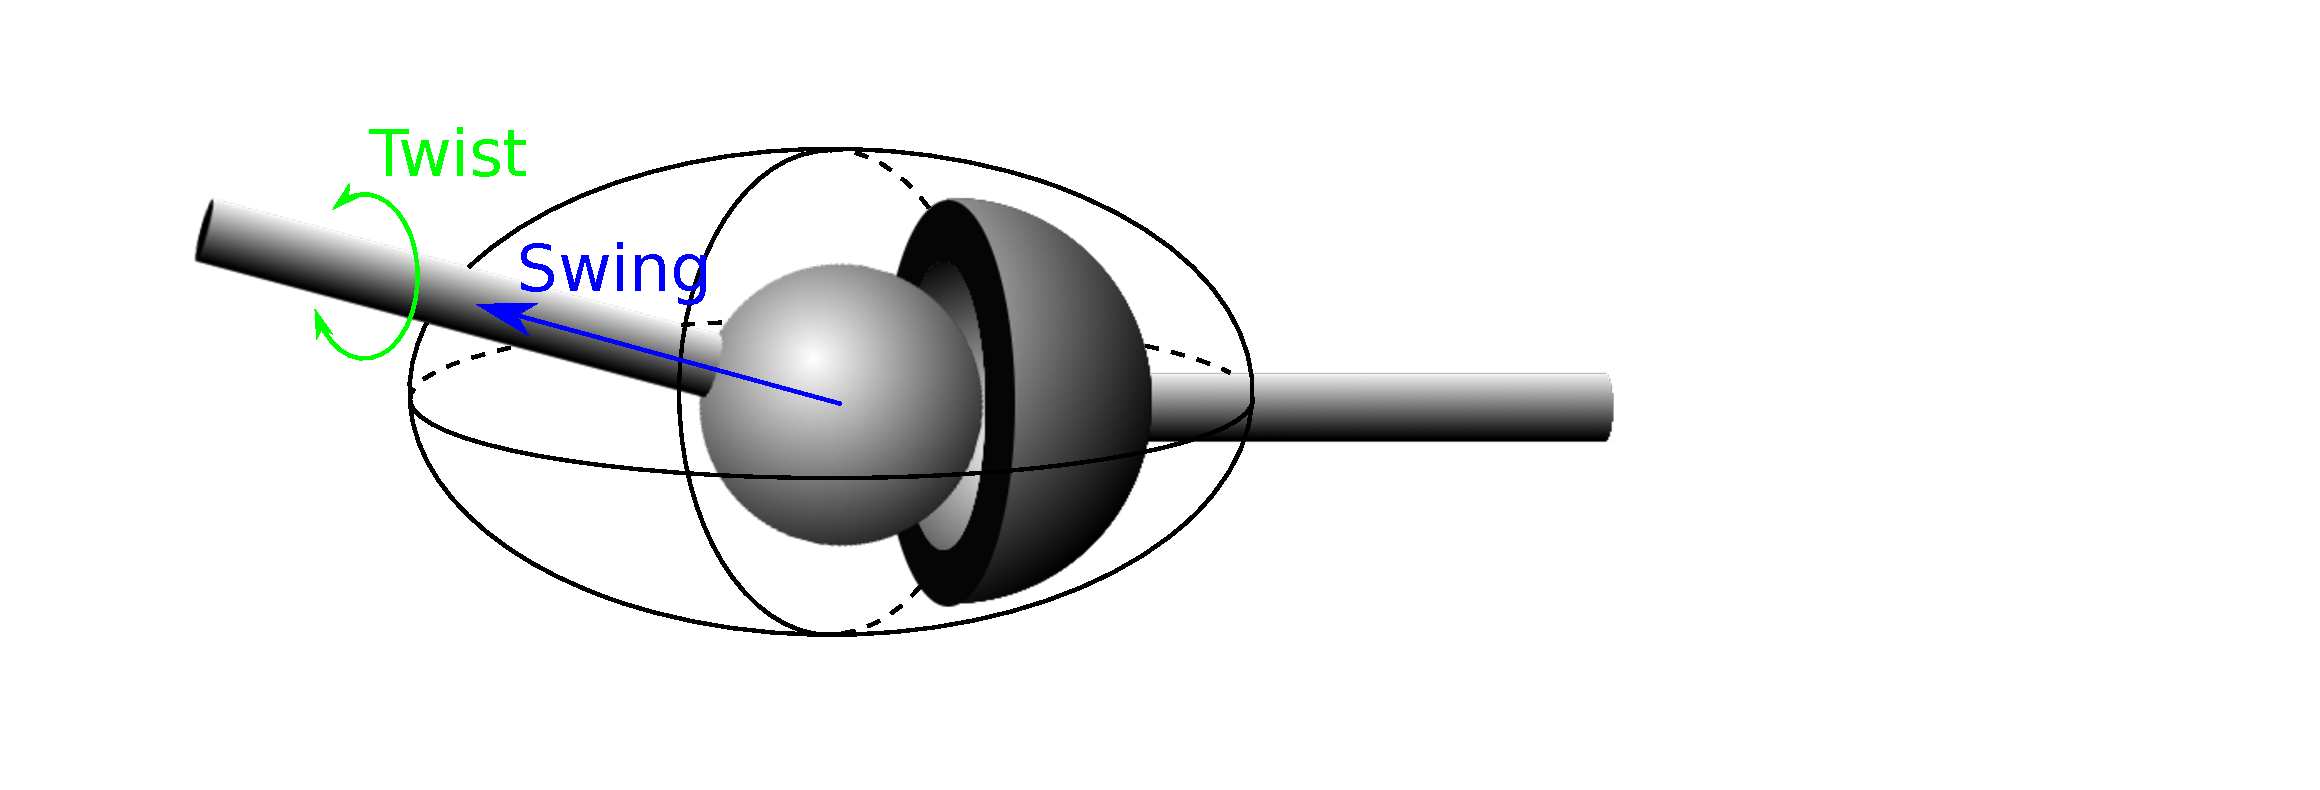
\includegraphics[width=0.7\linewidth]{ballAndSocket.pdf}
  \caption{Swing and Twist in ball and socket joint}
\label{fig:ballAndSocket}
\end{figure}

The spherical motion can be parameterized by a vector of the 3D unit sphere $S2$ and constrained to lay within a limit cone, the axial motion can be parameterized in $\mathbb{R}$ and limited by equation~\Eqref{eq:joint_limits}.
This type of formulation is presented in~\cite{baerlocher}.



\section{Contact constraints}
\label{sec:contact_constraints}

%%%%%%%%%%%%%%%%%%%%%%%%%%%%%%%%%%%%%%%%%%%%%%%%%%%%%%%%%%%%%%%%%%%%%%%
%                   SUBSECTION CONTACT CONSTRAINTS                    %
%%%%%%%%%%%%%%%%%%%%%%%%%%%%%%%%%%%%%%%%%%%%%%%%%%%%%%%%%%%%%%%%%%%%%%%

Humanoid robots evolve in their environment by making and breaking contacts with it.
A contact can be defined between 2 surfaces of different bodies of robots.
The most usual types of contact constraint encountered are the planar contact and the fixed contact.
A planar contact constraint is used when a planar surface of a robot is put in contact with a planar surface of the environment.
We denote $F_1 = \{O_1, \vec{x_1}, \vec{y_1}, \vec{z_1}\}$ a frame defined on $S_1$, the surface of the first body involved in the contact, such that the 3D point $O_1$ is on $S_1$ and the vector $\vec{z_1}$ is normal to $S_1$ and pointing toward the inside the body.
$F2 = \{O_2, \vec{x_2}, \vec{y_2}, \vec{z_2}\}$ is a frame on $S_2$, the surface of the second body involved, such that $O_2$ is on $S_2$ and the vector $\vec{z_2}$ is normal to $S_2$ and pointing away from the body.

Constraining $S_1$ and $S_2$ to be coplanar comes down to aligning $\vec{z_1}$ with $\vec{z_2}$ and to ensure that the projection of the distance between $O_1$ and $O_2$ along $\vec{z_1}$ is null.
Note that we avoid using the dot product of two vectors that are meant to be aligned e.g. $\vec{z_1}\cdot\vec{z_2} = 1$ because when that constraint is satisfied, its gradient is zero, which implies that in the optimization context it is unqualified.
That is why we prefer imposing orthogonality constraints.
This translates into adding the following set of constraints to our problem:

\begin{equation}
\label{eq:coplanarity}
\boxed{\left\{
  \begin{array}{l}
    \overrightarrow{O_1O_2} \cdot \vec{z_1} = 0\\
    \vec{x_1}\cdot\vec{z_2} = 0\\
    \vec{y_1}\cdot\vec{z_2} = 0\\
    \vec{z_1}\cdot\vec{z_2} \geq 0
  \end{array}
  \right.}
\end{equation}

This set of constraints leaves free the displacements of $F_2$ along $\vec{x_1}$ and $\vec{y_1}$ as well as its rotation around $\vec{z_1}$.
We call this a floating planar contact, the optimization algorithm will be able to choose the location of $F_2$ in the plane $\{O_1, \vec{x_1}, \vec{y_1}\}$.
This contact has 3 degrees of freedom.

\begin{figure}[htpb]
  \centering
  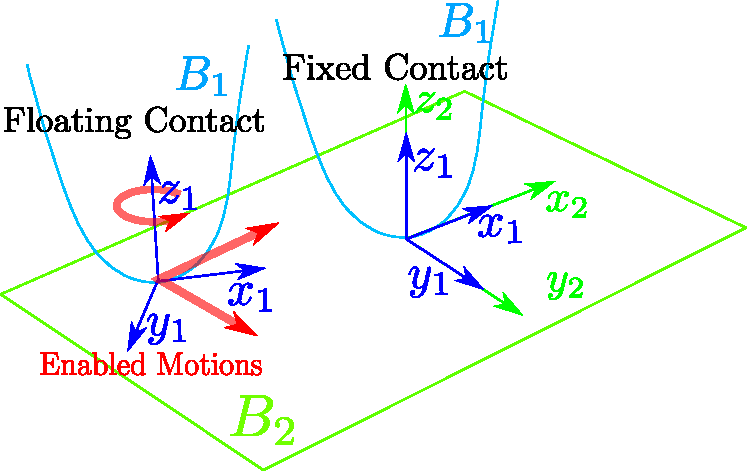
\includegraphics[width=0.8\linewidth]{contactConstraint.pdf}
  \caption{Floating and Fixed Contacts}
\label{fig:contactConstraint}
\end{figure}

If we constrain the location of $F_2$ in $\{O_1, \vec{x_1}, \vec{y_1}\}$ such that $O_1$ and $O_2$ are superimposed and $\vec{x_1}$, $\vec{y_1}$, $\vec{z_1}$ are aligned with respectively $\vec{x_2}$, $\vec{y_2}$, $\vec{z_2}$, we obtain a fixed contact with zero degrees of freedom.
This translates into adding the following set of constraints to our problem:

\begin{equation}
\label{eq:fixed_contact}
\boxed{\left\{
  \begin{array}{l}
    \overrightarrow{O_1O_2} = \vec{0}\\
    \vec{x_1}\cdot\vec{z_2} = 0\\
    \vec{y_1}\cdot\vec{z_2} = 0\\
    \vec{x_1}\cdot\vec{y_2} = 0\\
    \vec{z_1}\cdot\vec{z_2} \geq 0\\
    \vec{x_1}\cdot\vec{x_2} \geq 0\\
  \end{array}
  \right.}
\end{equation}

We illustrate those two types of contacts in~\Figref{fig:contactConstraint}



\section{Collision avoidance}
\label{sec:collision_avoidance}

%%%%%%%%%%%%%%%%%%%%%%%%%%%%%%%%%%%%%%%%%%%%%%%%%%%%%%%%%%%%%%%%%%%%%%%
%                   SUBSECTION COLLISION AVOIDANCE                    %
%%%%%%%%%%%%%%%%%%%%%%%%%%%%%%%%%%%%%%%%%%%%%%%%%%%%%%%%%%%%%%%%%%%%%%%

In order to avoid unwanted collisions between bodies of robots, for two bodies $B_1$ and $B_2$, we want to define a continuously differentiable function $d_{\{B_1, B_2\}}(q)$ that has the properties of a pseudo-distance:
\begin{itemize}
  \item $d_{\{B_1, B_2\}}(q) > 0$ when the bodies are not touching each other
  \item $d_{\{B_1, B_2\}}(q) = 0$ when the bodies are in collision without interpenetration
  \item $d_{\{B_1, B_2\}}(q) < 0$ when the bodies are in collision with interpenetration
\end{itemize}

Using the cartesian distance between the exact surfaces of $B_1$ and $B_2$ might result in a discontinuous gradient of $d_{\{B_1, B_2\}}$ if the surfaces of $B_1$ and $B_2$ are not strictly convex.
A conservative approach is to associate to each body, a strictly convex bounding volume and to compute the distance between those volumes.
\cite{escande:humanoids:2007} and~\cite{escande:itro:2014} proposes a method to generate a strictly convex Sphere-Torus-Patch Bounding Volumes (STP-BV) that guarantees the gradient continuity of the proximity distance.
The distance between the STP-BV of $B_1$ and $B_2$ computed by an enhanced GJK~\cite{gilbert-1988a} collision-detection algorithm is a continuously differentiable pseudo-distance.
Thus, we can use this function in our optimization algorithm to ensure that the distance between the bodies is greater than a safety distance $\epsilon_{12}$:

\begin{equation}
  \boxed{d_{\{B_1, B_2\}}(q) \geq \epsilon_{12}}
\end{equation}

This function can be used to avoid collisions between a robot and the environment as well as auto collisions between bodies of the same robot.
We denote $Coll$ the list of triplets $\{B_i, B_j, \epsilon_{ij}\}$ defining each collision that we want to avoid.

Then the set of constraints to add to our problem is:

\begin{equation}
  \boxed{\forall \{B_i, B_j, \epsilon_{ij}\} \in Coll,\ d_{\{B_i, B_j\}}(q) \geq \epsilon_{ij}}
\end{equation}

In many cases, it is possible to avoid the collision between two bodies of a robot by modifying the joint limits and reducing them to a span where the collision of interest cannot happen.
That approach is conservative and ad-hoc but can save some precious computation time.


%\section{Static constraints}
%\label{sec:static_constraints}

%%%%%%%%%%%%%%%%%%%%%%%%%%%%%%%%%%%%%%%%%%%%%%%%%%%%%%%%%%%%%%%%%%%%%%%
%                SECTION STATIC CONSTRAINTS                           %
%%%%%%%%%%%%%%%%%%%%%%%%%%%%%%%%%%%%%%%%%%%%%%%%%%%%%%%%%%%%%%%%%%%%%%%

\section{External Forces}
\label{sec:external_forces}

%%%%%%%%%%%%%%%%%%%%%%%%%%%%%%%%%%%%%%%%%%%%%%%%%%%%%%%%%%%%%%%%%%%%%%%
%                     SUBSECTION EXTERNAL FORCES                      %
%%%%%%%%%%%%%%%%%%%%%%%%%%%%%%%%%%%%%%%%%%%%%%%%%%%%%%%%%%%%%%%%%%%%%%%

For a robot to interact with the real world, its geometric description is not enough.
The robot is subject to forces applied on its bodies by the exterior world, which can be generated by contacts with the environment or with another actor (human, another robot, manipulated object\ldots), by the effect of physical forces like gravitation or magnetism, or by contacts between two bodies of the robot.
Our posture generator must take those `External forces' into account, to be able to estimate the stability of the robot and compute the internal torques generated in the joints.

An external force applied on a rigid body can also be called a wrench and is composed of a resultant part $f$ (sometimes called force) and a moment part (sometimes called couple).
Let $w$ be a wrench, $w|_F^O$ is the expression of $w$ calculated at the point $O$ expressed in the frame $F$.
We denote $\vec{f}$ the resultant part of w, and $\vec{f}|_F$ the expression of $\vec{f}$ in $F$.
$\vec{m}$ is the moment part of $w$ and $\vec{m}|_F^O$ the expression of $\vec{m}$ in $F$ calculated at the point $O$.

\begin{equation}
  w|_F^O = \left\{ \begin{array}{r}
    \vec{m}\\
    \vec{f}\\
  \end{array} \right\}^O_F
  = \left\{ \begin{array}{r}
    \vec{m}|_F^O\\
    \vec{f}|_F\\
  \end{array}\right\}
\end{equation}

The expression of the moment part on a different point $P$ is given by the following formula:

\begin{equation}
  \vec{m}|_F^P = \vec{m}|_F^O + \overrightarrow{PO} \wedge \vec{f}|_F
\end{equation}

The resultant part is invariant with respect to the point at which the wrench is calculated.

We drop the frame subscript when the choice of the frame does not matter and all quantities are computed in the same frame.



\section{Static stability}
\label{sec:static_stability}

%%%%%%%%%%%%%%%%%%%%%%%%%%%%%%%%%%%%%%%%%%%%%%%%%%%%%%%%%%%%%%%%%%%%%%%
%                    SUBSECTION STATIC STABILITY                      %
%%%%%%%%%%%%%%%%%%%%%%%%%%%%%%%%%%%%%%%%%%%%%%%%%%%%%%%%%%%%%%%%%%%%%%%

We denote $g$ the acceleration of gravity on earth $g = 9.81 m.s^{-2}$.
The wrench associated with the action of gravity on a body of mass $M$ which center of mass is denoted $G$ with $\vec{z}$ the upward vertical vector in the world frame $F_0$ is:
\begin{equation}
  w_g|^G_{F_0} = \left\{ \begin{array}{r}
     \vec{0} \\
     -Mg\vec{z} \\
 \end{array}\right\}^G_{F_0}
\end{equation}

A solid is statically stable if it satisfies the Euler-Newton Equation.
We consider a robot on which $m$ external wrench $w_i = \left\{ \begin{array}{r}
    \vec{m_i}\\
    \vec{f_i}\\
\end{array} \right\}^{P_i}$ are applied.
We denote $P$ the application point at which the equation and all its terms are calculated:
\begin{equation}
  \sum\limits_i w_i|^P + w_g|^P = 0
\end{equation}
which is equivalent to:
\begin{equation}
\left\{
\begin{array}{r}
  \sum\limits_i \vec{m_i}|^P + \overrightarrow{GP}\wedge Mg\vec{z} = 0 \\
  \sum\limits_i \vec{f_i} - Mg\vec{z} = 0 \\
\end{array}
\right.
\end{equation}

This equation can be simplified by applying it at the center of mass of the body as:
\begin{equation}
  \left\{
  \begin{array}{r}
    \sum\limits_i \vec{m_i}|^G = 0 \\
    \sum\limits_i \vec{f_i} - Mg\vec{z} = 0 \\
  \end{array}
  \right.
\label{eq:stability}
\end{equation}

Satisfying equation~\Eqref{eq:stability} ensures the stability of a rigid body.
If the robot's actuators are powerful enough to maintain its posture under any external perturbation, namely, when they can generate infinite or at least large enough torques, then the robot can be approximated as a rigid body and satisfying equation~\Eqref{eq:stability} is enough to ensure its stability.
%In some cases, an articulated robot is considered as a rigid body and this equation alone can be used to ensure its stability.
%It is only valid if the robot can generate infinite torques in its articulations, or at least if we have some guarantee that the robot is able to generate large enough torques.
Otherwise, it is necessary to verify that the robot's actuators can generate large enough torques to maintain that posture.
The details of torque computation are discussed in Section~\ref{sec:torque_limits}

Equation~\Eqref{eq:stability} can be used in an optimization problem.
We consider that each wrench $w_i$ applied on the system is defined by the position of its application point $P_i$ and the values $m_i$ and $f_i$ that represent the moment and resultant of $w_i$ at $P_i$.
$P_i$ depends on $q$ the joint parameter of the robot.
$m_i$ and $f_i$ are new variables that need to be added to the problem.
In summary, $w_i$ depends on $q$, $m_i$ and $f_i$.
We denote $f$ the concatenation of all the variables $m_i$ and $f_i$.

\begin{equation}
  \boxed{s(q,f) = \left\{
  \begin{array}{r}
    \sum\limits_i \vec{m_i} + \overrightarrow{P_i G}\wedge \vec{f_i} \\
    \sum\limits_i \vec{f_i} - Mg\vec{z} \\
  \end{array}
  \right\}
  = 0}
\end{equation}

The optimization problem~\Eqref{eq:optim_form_PG} becomes (we denote m the dimension of the force variables):

\begin{equation}
\label{eq:optim_form_PG_with_stab}
  \left\{
  \begin{array}{l}
    \min\limits_{q\in\mathcal{C}, f\in \mathbb{R}^m}{f(q)}\\
    \text{ s.t. }
    \left\{
    \begin{array}{l}
      s(q,f) = 0\\
      c_i(q) = 0,\ \forall i\in{E}\\
      c_i(q) \geq 0,\ \forall i\in{I}\\
    \end{array}
    \right.
  \end{array}
  \right.
\end{equation}

The derivation of the static stability constraint is straightforward.
All the terms of equation~\Eqref{eq:stability} are components of wrenches.
A wrench is completely defined by the frame in which it is expressed and its values of resultant and moment in that frame.
Deriving the stability condition comes down to deriving each term w.r.t its components values and w.r.t the transformation of its frame.

\begin{equation}
\left\{
\begin{array}{r}
  \partial\left(\sum\limits_i m_i|^G\right) = \sum\limits_i \partial(m_i|^G) \\
  \partial\left(\sum\limits_i f_i\right) = \sum\limits_i \partial(f_i) \\
\end{array}
\right.
\label{eq:derivation_stability}
\end{equation}

We will explicit a method to automatically compute those derivatives in a further chapter.



\section{Center of mass projection}
\label{sec:center_of_mass_projection}

%%%%%%%%%%%%%%%%%%%%%%%%%%%%%%%%%%%%%%%%%%%%%%%%%%%%%%%%%%%%%%%%%%%%%%%
%                SUBSECTION CENTER OF MASS PROJECTION                 %
%%%%%%%%%%%%%%%%%%%%%%%%%%%%%%%%%%%%%%%%%%%%%%%%%%%%%%%%%%%%%%%%%%%%%%%

When all the wrenches applied to the body are due to unilateral punctual contacts on the same horizontal plane $H = \{O, \vec{x}, \vec{y}\}$, the stability criterion~\Eqref{eq:stability} can be simplified.
The wrench $w_i$ generated by a unilateral punctual contact is a pure force resultant, its moment part is zero on the contact point.

\begin{equation*}
    \left. w_i \right|^{P_i} =
    \left\{
      \begin{array}{r}
      \vec{0}\\
      \vec{f_i}\\
  \end{array} \right\}^{P_i}
\end{equation*}

Equation~\Eqref{eq:stability} becomes:

\begin{equation}
\left\{
\begin{array}{r}
  \sum\limits_i \overrightarrow{OP_i}\wedge \vec{f_i} - \overrightarrow{OG} \wedge Mg\vec{z} = 0 \\
  \sum\limits_i \vec{f_i} - Mg\vec{z} = 0 \\
\end{array}
\right.
\end{equation}

We can write $\overrightarrow{OG} = \overrightarrow{OG_p} + z_G\vec{z}$ with $G_P$ the projection of $G$ on $H$. Replacing in the moment equation gives:

\begin{equation}
  \sum\limits_i \overrightarrow{OP_i}\wedge \vec{f_i} - \sum\limits_i\overrightarrow{OG_P} \wedge \vec{f_i} = 0
\label{eq:projCoM}
\end{equation}

With $f_i = f_i^x\vec{x} + f_i^y\vec{y} + f_i^z\vec{z}$, $G$ and $P_i$ can be written as $\overrightarrow{OG_P} = G_x \vec{x} + G_y\vec{y}$ and $\overrightarrow{OP_i} = P_{ix} \vec{x} + P_{iy} \vec{y}$. The two first lines of equation~\Eqref{eq:projCoM} give:

\begin{align}
\sum\limits_i \left\{\begin{array}{r} P_{iy}f_i^z\\-P_{ix}f_i^z\end{array}\right\}
= \left\{\begin{array}{r} G_{y}\\-G_{x}\end{array}\right\} \sum\limits_i f_i^z\\
  \overrightarrow{OG_P} = \frac{\sum\limits_i \overrightarrow{OP_i} f_i^z}{\sum\limits_i f_i^z}
\end{align}

Since all the contacts are unilateral, all the $f_i^z$ are positive.
For any set of $f_i^z\geq0$, $G_P$ is a barycenter with positive coefficients of the $P_i$.
Any point $G_P$ that is included in the convex hull of all the $P_i$ is a solution.

Thus, we have the property: a rigid body that has all its contacts with the environment being punctual, unilateral and all lying on the same horizontal plane $H$ is stable if and only if the projection of its center of mass on $H$ is inside the convex hull of all its contact points.



\section{Torque limits}
\label{sec:torque_limits}

%%%%%%%%%%%%%%%%%%%%%%%%%%%%%%%%%%%%%%%%%%%%%%%%%%%%%%%%%%%%%%%%%%%%%%%
%                      SUBSECTION TORQUE LIMITS                       %
%%%%%%%%%%%%%%%%%%%%%%%%%%%%%%%%%%%%%%%%%%%%%%%%%%%%%%%%%%%%%%%%%%%%%%%

In general, satisfying equation~\Eqref{eq:stability} is not enough to ensure that a robot can be statically stable.
The joint torques that are required to hold the posture must be within the physical capabilities of the robot, namely, its torque limits.
We denote $\tau_i^-$ and $\tau_i^+$ the minimal and maximal torques that can be generated by the robot's actuators on joint $J_i$.
In some cases, the torque limits can depend on the joint parameters $\tau_i^-(q)$ and $\tau_i^+(q)$.
For example, it is the case with the Atlas robot that is hydraulically actuated.

Featherstone~\cite{featherstone:book:2007} proposes a recursive algorithm to compute the torques, accelerations, and velocities generated in a multi-articulated system by a set of external forces called the Inverse Dynamics Algorithm.
For the purpose of generating statically stable postures, the velocities and accelerations are useless.
Thus, we devise a specialized algorithm to fit our needs and call it the Inverse Static Algorithm.

We denote $a_g$ the gravity acceleration vector with $\vec{a_c}$ its rotation part and $\vec{a_f}$ its translation part:
\begin{equation}
  a_g = \left\{ \begin{array}{r}
    \vec{a_c} \\
    \vec{a_f} \\
  \end{array} \right\}
  = \left\{ \begin{array}{r}
    \vec{0} \\
    g\vec{z}\\
  \end{array} \right\}
\end{equation}

The algorithm first computes the generalized forces $f^G_i$ applied to each body.
It is the sum of the action of gravity and of the external forces applied on a body calculated at the origin of the world frame, expressed in the world frame.
Then, the generalized forces are used to compute the torques.
We denote $\mathbf{I}_i$ the inertia matrix of body $i$.

\begin{algorithm}
  \caption{Inverse Static Algorithm}
\label{alg:IS}
\begin{algorithmic}
  \For{$i = 0:n_B$}
  \State$f^G_i = \mathbf{I}_i {}^i\mathbf{X}_0 a_g - {{}^i\mathbf{X}_0}^*f_i^{ext}$
  \EndFor{}
  \For{$i = n_J-1:0$}
  \State$\tau_i = {f^G_i}^T S_i$
  \If{$pred(i) \neq -1$}
  \State$f^G_{pred(i)} += {\mathbf{X}^{PtS}_i(q)}^{-*} f^G_i$
  \EndIf{}
  \EndFor{}
\end{algorithmic}
\end{algorithm}

We can write the torques as a function of the joint parameters and the external forces $\tau(q,f)$.
The torque limit constraint writes as:
\begin{equation}
  \boxed{\tau^- \leq \tau(q,f) \leq \tau^+}
\end{equation}

We will detail the derivation of this constraint in Section~\ref{sec:torque_derivation}.


\section{Contact Forces and Friction Cones}
\label{sec:contact_forces_and_friction_cones}

%%%%%%%%%%%%%%%%%%%%%%%%%%%%%%%%%%%%%%%%%%%%%%%%%%%%%%%%%%%%%%%%%%%%%%%
%            SUBSECTION CONTACT FORCES AND FRICTION CONES             %
%%%%%%%%%%%%%%%%%%%%%%%%%%%%%%%%%%%%%%%%%%%%%%%%%%%%%%%%%%%%%%%%%%%%%%%

%Here we use the same frames and notations as introduced in Section~\ref{sec:contact_constraints}.

The contacts involved in a posture generation problem can be separated into two types: Geometric Contacts and Stability Contacts.

The Geometric Contact is a contact where the position of contact is reached, but that contact does not support any contact forces (this is a necessary step to generate a sequence of quasi-static transitions).
Physically, that correspond to the transition state between a configuration without contact and a configuration with contact on which forces are applied.
We defined the Geometric Contacts in Section~\ref{sec:contact_constraints}.
The Stability Contact is a Geometric Contact that bears interaction forces.

%In planning, contacts are added or removed one by one between successive postures.
%In order to add or remove a stability contact, it is necessary to go through a geometric contact (that guarantees the continuity on contact forces).
%First a geometric contact configuration is found, then on the next posture, that geometric contact is fixed ond forces are added on it, it becomes a stability contact.
%Similarly, to remove a stability contact, we first look for a posture with a fixed geometric contact in place of the stability contact to remove.
%And on the next posture, the contact can be removed.

We denote $w_{1\rightarrow 2}$ the force applied by body $B_1$ on body $B_2$.
Then the force applied by $B_2$ on $B_1$ is $w_{2\rightarrow 1} = -w_{1\rightarrow 2}$.
%These interaction forces must be taken into account in the stability and torque computations of each robot involved in the contact.

The interaction force resulting from a punctual contact (see~\Figref{fig:frictionCone}) on a point $P$ can be modeled as a pure force resultant along the $z_1$ direction $\vec{f_n} = f_z \vec{z_1}$ and the tangential efforts due to the friction in that contact can be modeled as $\vec{f_t} = f_x \vec{x_1} + f_y \vec{y_1}$.
%A punctual contact cannot carry moments on its contact point.

\begin{equation}
\label{eq:punctual_force}
\left. w_{2\rightarrow 1}\right|^P = \left\{
  \begin{array}{l}
    \vec{0} \\
    \overrightarrow{f_{2\rightarrow 1}} = \vec{f_t} + \vec{f_n} \\
  \end{array}
  \right\}^P
\end{equation}

\begin{figure}[htpb]
  \centering
  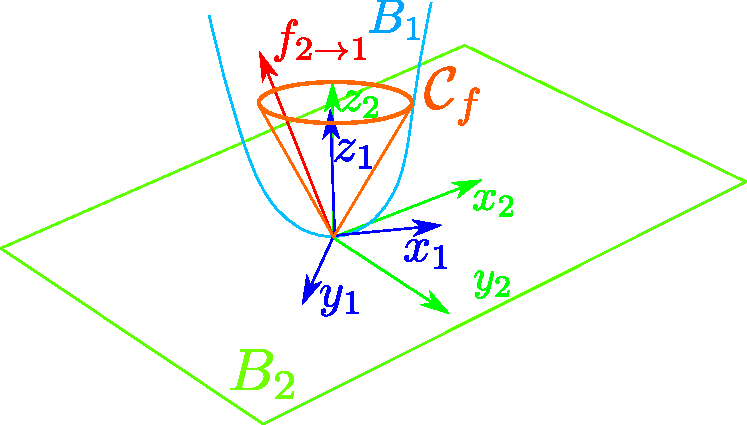
\includegraphics[width=0.6\linewidth]{frictionCone.pdf}
  \caption{Punctual unilateral stability contact with friction}
\label{fig:frictionCone}
\end{figure}

This formulation of the interaction force defines a bilateral contact, in the sense that the force can be in any direction, $B_1$ can push as well as pull on $B_2$.

To model a unilateral contact, we must constrain the normal component of $f_{2\rightarrow 1}$ to be oriented toward the inside of $B_1$.
This means that only pushing actions can be generated, not pulling actions.
This translates into:
\begin{equation}
  \overrightarrow{f_{2\rightarrow 1}}\cdot \vec{z_1} = f_z \geq 0
\end{equation}

Furthermore, to avoid slippage, the Coulomb friction law must be respected for each contact force $\vec{f}$.
%This law states that the contact force resultant must lay inside a friction cone of angle $\mu$, the friction coefficient.
Which translates into the following equation, with $\vec{f_n}$ and $f_t$, respectively the normal and tangential parts of $\vec{f}$ and $\mu$, the friction coefficient:

\begin{equation}
  \mu\|\vec{f_n}\| \geq \|\vec{f_t}\|
\end{equation}

Given the decomposition of $f_{2\rightarrow 1}$ in $F_1$, $f_{2\rightarrow 1} = f_x \vec{x_1} + f_y \vec{y_1} + f_z \vec{z_1}$, for any punctual contact in a posture generation problem, we can add the following set of constraint to our optimization problem:

\begin{equation}
  \label{eq:unilateralContact}
  \left\{
  \begin{array}{l}
    f_z \geq 0 \\
    \mu^2 f_z^2 - f_x^2 +f_y^2 \geq 0
  \end{array}
  \right.
\end{equation}

When it comes to planar contacts on surface $S$ with $\vec{n}$ the outbound normal to $S$, the interaction force can have components of forces and moments in all directions.
The forces components intrinsic to the planar contact model are a resultant part aligned with $\vec{n}$ $\vec{f_n} = f_z \vec{z_1}$ and a moment part tangential to $S$: $\vec{m_t} = m_x \vec{x_1} + m_y \vec{y_1}$.
The forces due to friction are a tangential friction resultant part $\vec{f_t} = f_x \vec{x_1} + f_y \vec{y_1}$ and a normal friction moment $\vec{m_n} = m_z \vec{z_1}$.

This type of force can be modeled by a set of unilateral punctual efforts applied on each vertex of a polygon describing the contact area.
And ensuring that each of them lay in their respective friction cone, thus satisfying the equation~\Eqref{eq:unilateralContact}.
As depicted in~\Figref{fig:planarContact}

\begin{figure}[htpb]
  \centering
  \setlength{\fboxsep}{0pt}%
  \setlength{\fboxrule}{1pt}%
  \fbox{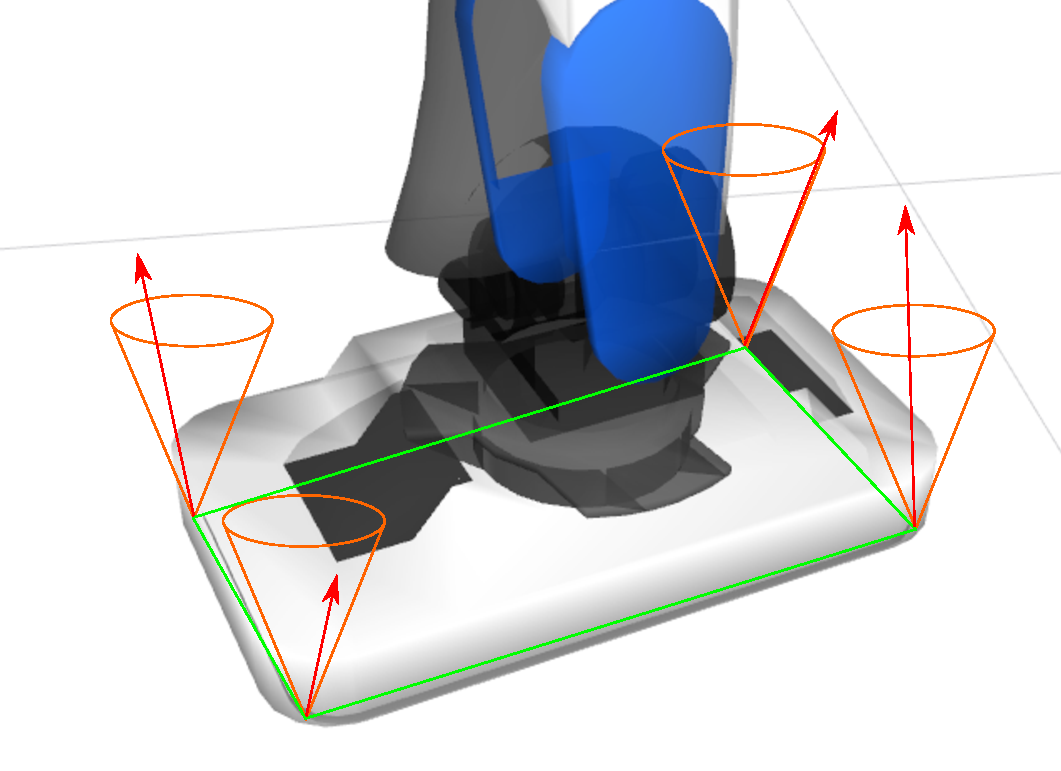
\includegraphics[width=0.6\linewidth]{planarContact.pdf}}
  \caption{Modelization of a Planar Contact between the foot on HRP4 and the ground}
\label{fig:planarContact}
\end{figure}



\section{Cost Functions}
\label{sec:cost_functions}

%%%%%%%%%%%%%%%%%%%%%%%%%%%%%%%%%%%%%%%%%%%%%%%%%%%%%%%%%%%%%%%%%%%%%%%
%                       SECTION COST FUNCTIONS                        %
%%%%%%%%%%%%%%%%%%%%%%%%%%%%%%%%%%%%%%%%%%%%%%%%%%%%%%%%%%%%%%%%%%%%%%%

In addition to constraints, it is often useful to add a cost function to our optimization problem.
The submanifold of feasible configurations $\mathcal{C}_F$ can contain an infinity of solutions and even some continuous solution areas in which all points are solutions.
The cost function helps to choose the `best' candidate solution.
Various types of cost functions can be chosen, for example, we can minimize the distance to a reference posture $q_R$:

\begin{equation*}
  f_\text{posture}(q) = {\|q-q_R\|}^2
\end{equation*}

The effect of that type of cost function is illustrated in~\Figref{fig:cost}.
On both images, the HRP-2 Kai robot is stable, respects its joints and torques limits.
The only difference is that the right one minimizes the distance to a reference posture (standing straight with bent knees) while the left result does not use a cost function.

\begin{figure}[htpb]
  \centering
  \setlength{\fboxsep}{0pt}%
  \setlength{\fboxrule}{1pt}%
  \fbox{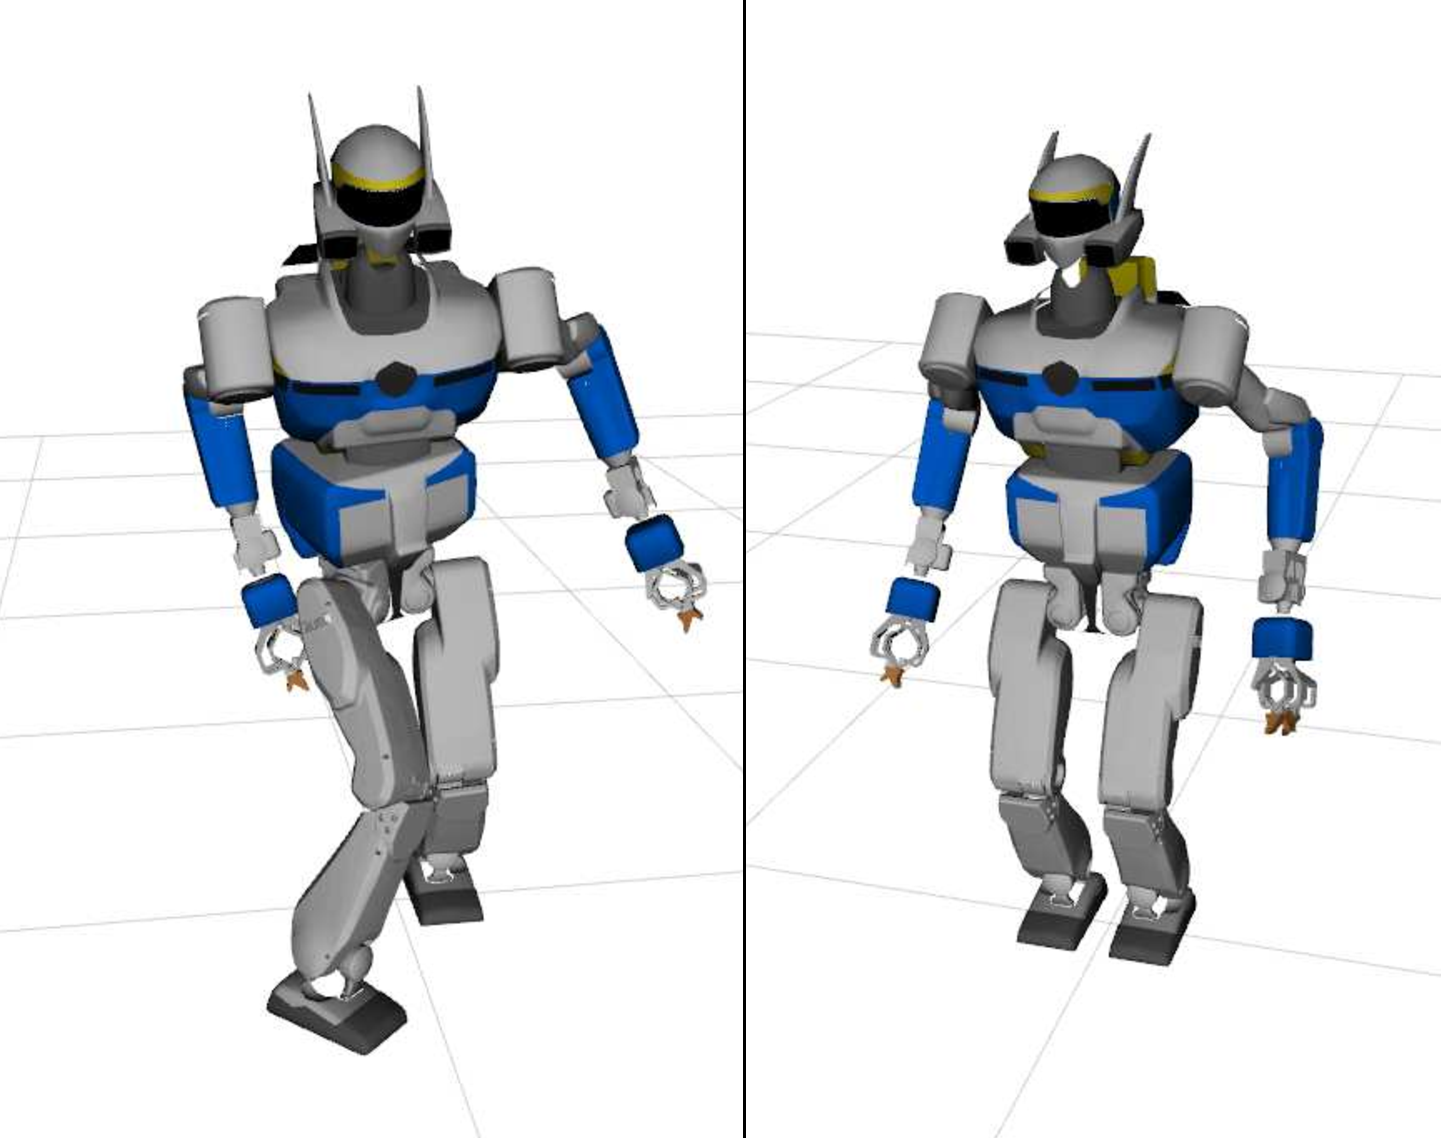
\includegraphics[width=0.5\linewidth]{cost.pdf}}
  \caption{Effect of cost function. Left: no cost function. Right: Distance to posture}
\label{fig:cost}
\end{figure}

We can also want to minimize the sum of norms of contact forces:
\begin{equation*}
  f_\text{forces}(f) = \sum\limits_i {\|f_i(f)\|}^2
\end{equation*}
or the torques in the robot's joints:
\begin{equation*}
  f_\text{torques}(q,f) = \sum\limits_i {\|\tau_i(q,f)\|}^2
\end{equation*}
Some more custom cost functions can also be considered, for example, we may want a point $P_i$ on body $B_i$ with to be as far as possible in a direction $\vec{d}$
\begin{equation*}
  f_\text{point} (q) = -{\overrightarrow{O_0 P_i}}\cdot{\vec{d}}
\end{equation*}

Any positively weighted combination of cost function can be used, in which case it is important to choose the weights $p_i$ carefully to scale all the costs so that they all can influence the result and none is completely dominated by another.
\begin{equation}
  f_\text{cost}(q,f) = \sum\limits_i{p_i f_i(q,f)} = p_0 f_\text{posture}(q) + p_1 f_\text{forces}(f) + p_2 f_\text{torques}(q,f) + \cdots
\end{equation}



\section{Conclusion}
\label{sec:Ch1_Conclusion}

%%%%%%%%%%%%%%%%%%%%%%%%%%%%%%%%%%%%%%%%%%%%%%%%%%%%%%%%%%%%%%%%%%%%%%%
%                         SECTION CONCLUSION                          %
%%%%%%%%%%%%%%%%%%%%%%%%%%%%%%%%%%%%%%%%%%%%%%%%%%%%%%%%%%%%%%%%%%%%%%%

In this section, we have seen how to formulate a robotics problem with several different tasks and objectives as an optimization problem.

We denote $\mathcal{T}_i$ the additional tasks added to the problem, which is described by the set of equations $g_i(q,f) = 0$ and inequations $h_i(q,f) \geq 0$.
The contact tasks are included in those and the equations describing them must encompass the geometric contact constraint equation like~\Eqref{eq:coplanarity} as well as the unilaterality and friction equations~\Eqref{eq:unilateralContact} in the case of a unilateral contact.

A typical robotics problem can be written as a combination of all those costs and constraints:
\begin{align}
\minimize_{q, f} & \quad f_\text{cost}(q,f) \nonumber\\
\text{s.t.}&
\left\{
\begin{array}{lr}
q^- \le q \le q^+\\
s(q,f) = 0 \\
\tau^- \le \tau(f,q) \le \tau^+\\
\forall \{B_i, B_j, \epsilon_{ij}\} \in Coll,\ d_{\{B_i, B_j\}}(q) > \epsilon_{ij}\\
g_i(q,f) = 0\ \ \forall\mathcal{T}_i,\\
h_i(q,f) \geq 0\ \ \forall\mathcal{T}_i.
\end{array}\right.
\label{eq:PG}
\end{align}

In the next chapter, we present an extension to the contact constraint formulation that allows generating non-inclusive contacts, an algorithm to compute the exact derivatives of the torques in robot's joints, and our endeavor to apply a different optimization approach to solving posture generation problems.


%%%%%%%%%%%%%%%%%%%%%%%%%%%%%%%%%%%%%%%%%%%%%%%%%%%%%%%%%%%%%%%%%%%%%%%
%                           Second Chapter                            %
%                  Extensions of Posture Generation                   %
%%%%%%%%%%%%%%%%%%%%%%%%%%%%%%%%%%%%%%%%%%%%%%%%%%%%%%%%%%%%%%%%%%%%%%%

\chapter{Extensions of Posture Generation}
\label{cha:extensions_of_posture_generation}

\graphicspath{{Chapter3-Extensions/Figs/}{Chapter3-Extensions/Figs/IROS14/}}

%Intro
In this chapter, we present three different and unrelated contributions to the state of the art of posture generation.
First, we present a novel method called Integration of Non-Inclusive Contacts in Posture Generation that was published in~\cite{brossette:iros:2014}.
Second, we present a generic algorithm to compute efficiently the derivative of the joint torques of a robot.
Third, we present our endeavor to apply an optimization method called `Lifted Newton Method', presented in~\cite{Albersmeyer:2010:LNM:1958447.1958472}, to problems of inverse kinematics.

%{{{ SECTION: List of contributions

%\section{List of contributions}
%%%%%%%%%%%%%%%%%%%%%%%%%%%%%%%%%%%%%%%%%%%%%%%%%%%%%%%%%%%%%%%%%%%%%%%%

%%                  SECTION LIST OF CONTRIBUTIONS                      %
%%%%%%%%%%%%%%%%%%%%%%%%%%%%%%%%%%%%%%%%%%%%%%%%%%%%%%%%%%%%%%%%%%%%%%%%

%\begin{itemize}
  %\item The method presented before is limiting in many cases. Ladder, stairs climbing\dots.
%Sometimes it is not possible to ensure inclusion of 2 surfaces.
  %\item Contact geometry formulation
    %\begin{itemize}
      %\item Discretisation of contact surfaces for practical reasons
      %\item Contact generation with convex surface inclusions
%Usual methods for generating surface contact are based on point-to-point sampling, on rectangular inclusion, or other limiting methods. We extend that to the inclusion of convex surfaces.
      %\item Inclusive contacts are no problem
      %\item Non-Inclusive contacts lead to non-constant number of constraints or non-smooth gradients, cannot be solved with usual solvers with that formulation
    %\end{itemize}
  %\item{Non inclusive contact constraints}
    %\begin{itemize}
      %\item {Main Idea: Inserting an ellipse in the intersection of polygons}
      %\item {Pseudo-distance (to simplify the formulation)}
      %\item {Modification of the optimization problem}
      %\item {Maximization of the contact area}
      %\item {Using non inclusive contact to maintain stability}
      %\item {Extension to singular cases}
    %\end{itemize}
  %\item{Simulation Results}
    %\begin{itemize}
      %\item{Inclined ladder climbing}
      %\item{Vertical ladder climbing}
      %\item{Climbing Stairs}
      %\item{Walking along a path made of small objects}
    %\end{itemize}
  %\item{Application to ladder climbing (cf. Joris papers)}
%\end{itemize}

%\paragraph{Torque Derivation}

%\paragraph{On the use of lifted variables for Robotics Posture Generation}
%\begin{itemize}
  %\item {Introduction: `J. Albersmeyer and M. Diehl, The lifted Newton Method and its Application in Optimisation'}
  %\item {Lifting Algorithm: Introduce additional variables to reduce the complexity/degree of the equations to solve. And then use a trick to re-condense the system and avoid loosing computation time}
  %\item {Optimization on lifted variables}
  %\item {Condensed BFGS update}
  %\item {Results, experimentation}
  %\begin{itemize}
    %\item Symbolic Inverse Kinematics
    %\item Automatic Lifting algorithm adapted to posture generation
    %\item Several Solvers for lifted and non-lifted systems (Gauss-Newton, SQP, lifted Newton\ldots)
    %\item Compared many optimization methods (Globalization, regularization\ldots)
    %\item Never managed to get results faster than basic methods
  %\end{itemize}
  %\item{Motivation:Development of a posture generator with a specialized solver}
    %\begin{itemize}
      %\item Problem
        %\begin{itemize}
          %\item Robotics problems solved with generic solvers (IPOPT, CFSQP, fmincon\ldots)
          %\item Robotics problems (especially posture generation) are very specific (Constraints, costs, working spaces, sizes\ldots)
        %\end{itemize}
      %\item Solution
        %\begin{itemize}
          %\item Develop a posture generator, along with a nonlinear solver
          %\item Better understanding of our own solver
          %\item Ability to use the solver in new ways:
          %\begin{itemize}
            %\item Working on Manifolds
            %\item Variable numbers of constraints
            %\item Automatic management of variables, constraints and mathematical expressions
          %\end{itemize}
        %\end{itemize}
    %\end{itemize}
%\end{itemize}
%}}}
\section{Integration of Non-Inclusive Contacts in Posture Generation}
\label{sec:integration_on_non_inclusive_contacts_in_posture generation}

%%%%%%%%%%%%%%%%%%%%%%%%%%%%%%%%%%%%%%%%%%%%%%%%%%%%%%%%%%%%%%%%%%%%%%%%%
%  SECTION INTEGRATION ON NON-INCLUSIVE CONTACTS IN POSTURE GENERATION  %
%%%%%%%%%%%%%%%%%%%%%%%%%%%%%%%%%%%%%%%%%%%%%%%%%%%%%%%%%%%%%%%%%%%%%%%%%

In Section~\ref{sec:contact_constraints}, we defined a set of constraints (equations~\Eqref{eq:coplanarity}) that ensures the coplanarity of two planar surfaces in a geometric contact.
Those equations guarantee the coplanarity of two infinite planar surfaces.
Another set of constraints needs to be added to ensure the validity of a contact between two bounded surfaces $S_1$ and $S_2$, to ensure that their intersection is not empty and that it is large enough to support the contact.

We propose a simple way to formulate geometric contact formation to have an arbitrary intersection shape that we apply to a robotic (humanoid) posture generation problem, when searching for a contact between two surfaces.
We start by defining convex areas of contact on the robot's body and the environment, that we call \emph{contact patches}.
We can generate contacts with an arbitrary intersection of a pair of any of these predefined contact patches.
Virtually any planar surface can be a contact patch.
In our group's previous works, the constraints formulating a new contact in the posture generator, states that a contact patch is totally included into another, which is obviously a limitation of the posture generation.
A simple example is when a human climbs stairs. S/he usually contacts only the front half of its foot with each step, the heel almost never touches the steps.
Our new geometric contact modeling writes very simply as additional constraints and variables added to the optimization problem. It consists of searching for an ellipse inscribed in the intersection of the pair of patches we want in contact.
The result of our posture generator is then a configuration where contact patches are not necessarily included in one another (therefore we named it non-inclusive) and the shape and area of their intersection can be monitored.
This allows our posture generator to propose contacts of different shapes with a non-predefined number of contact points (used later to compute reaction/contact forces).
We illustrate the efficiency of our method in multi-contact posture generation with the HRP-2 and ATLAS humanoid robots with results that can not be generated automatically by existing methods.

\begin{figure}
\centering
  \centering
  \setlength\fboxsep{0pt}
  \setlength\fboxrule{1pt}
  \fbox{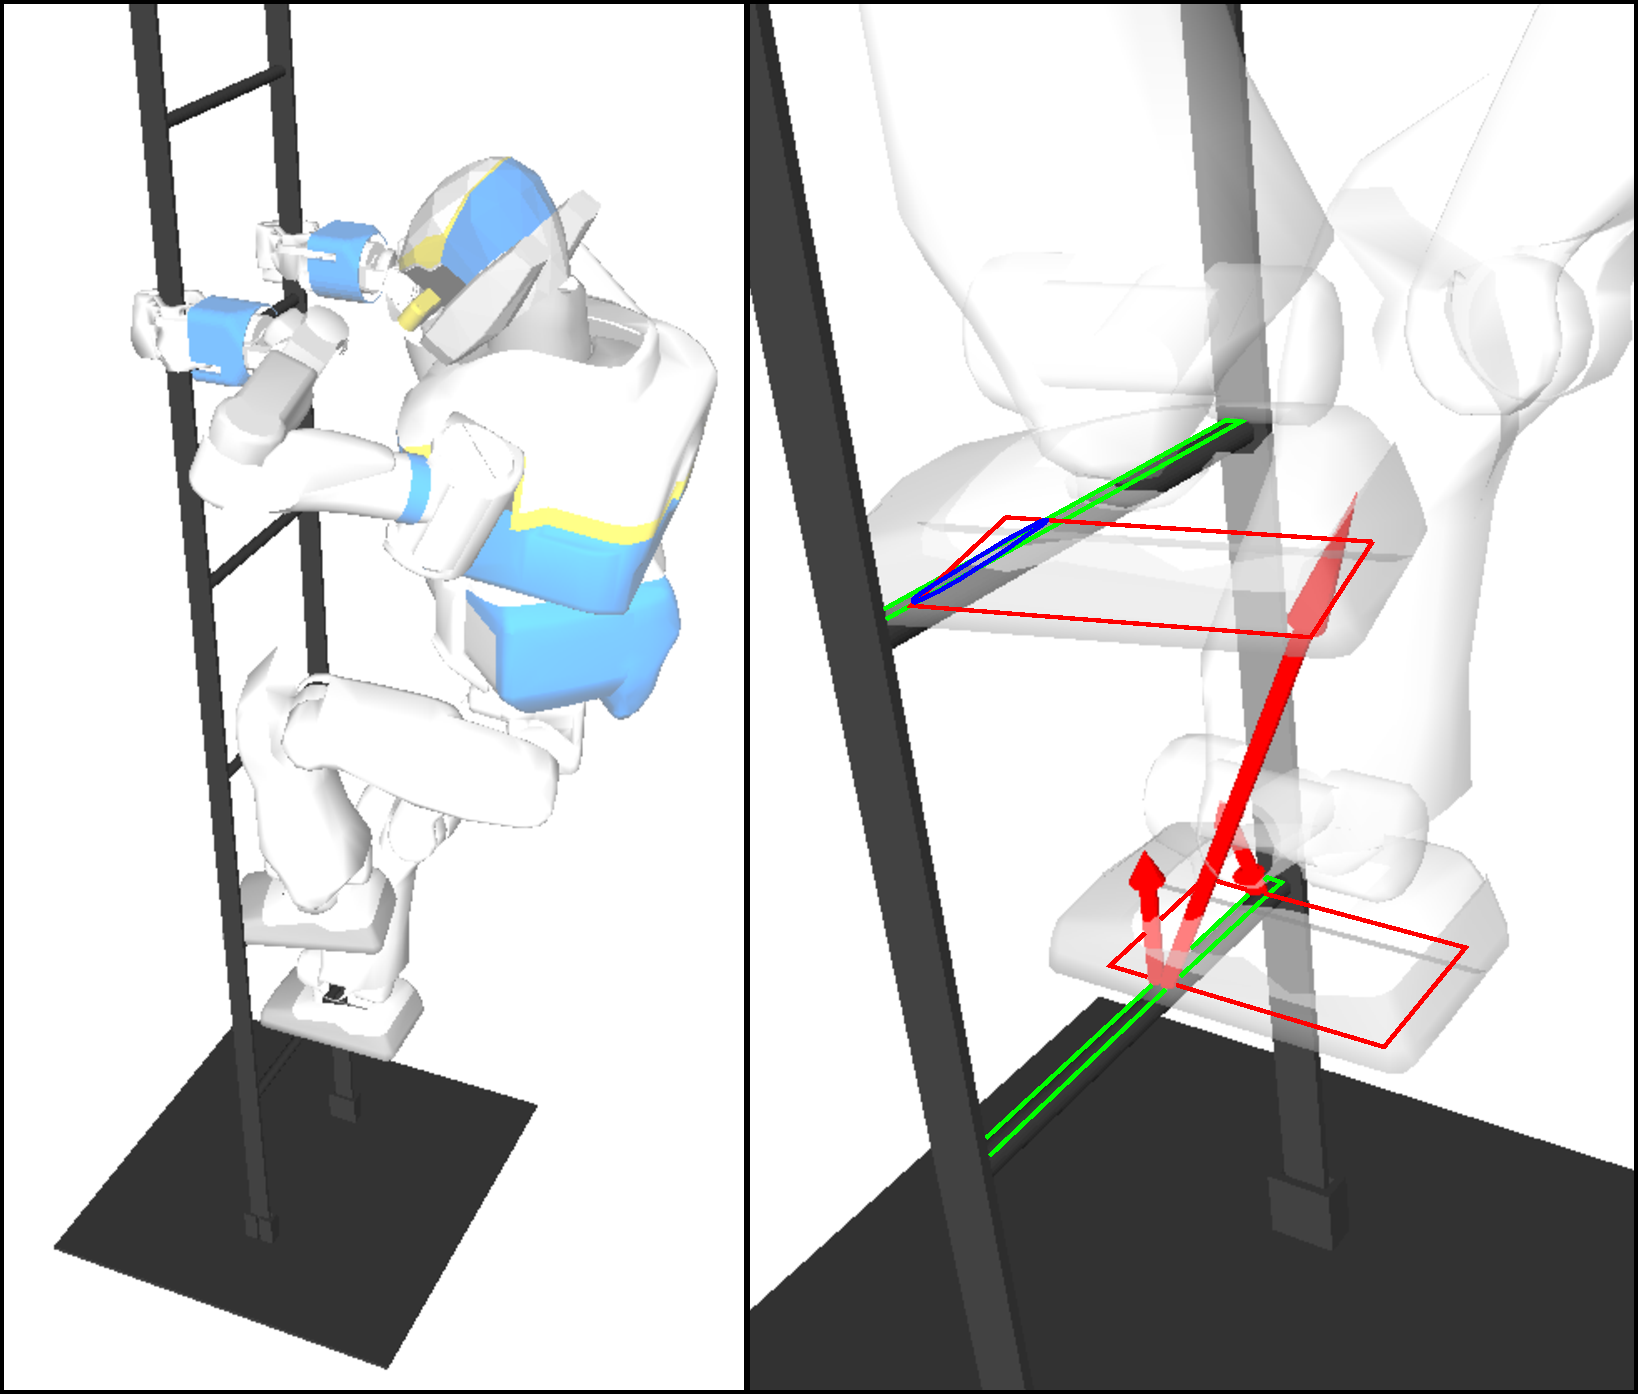
\includegraphics[width=.55\linewidth]{hrp2_ladder_jrl_5_combo.pdf}}
\caption{Using non-inclusive contacts for ladder climbing (green/red: contact polygons; blue: contact ellipse; red arrows: contact forces resultants)}
\label{fig:hrp2_jrl_complete}
\end{figure}

%In general, desired contacts write as hard constraints to fulfill in an optimization problem.
%Yet, we need to write the maths for, say, put the gripper on the wall and the left foot on the ground.
%In general, the maths of a gripper is a complex geometric description, so is often that of the environment.
A contact is generally defined by a pair of points (one on each object in contact) and a normal vector.
A contact constraint consists in finding a posture in which the predefined authorized contact points and normal of each body match~\cite{zhang:TePRA:2013}\cite{hauser:ijrr:2008}.
Likewise, in~\cite{osswald:iros:2011}, the position of the feet of the NAO robot is manually tuned in order to obtain statically stable position during the climbing of a spiral staircase.
In~\cite{Chestnutt:2009:BNR:1733023.1733314}, the surface in contact is chosen according to two criteria: the position of the force sensors of the feet, and the desired contact.
In~\cite{sentis:itro:2010}, the problem of contact discovery in not considered.
In~\cite{mordatch:acm:2012}, two surfaces are considered in contact as soon as the center point of one of them touches the other one and their normals match.
Although used in many papers, it is not difficult to see that this definition of contact excludes a series of possibilities that would have been obtained if the predefined points were placed in different configurations within their respective patches.
Table~\ref{tbl:contact_description} presents some diagrams describing some typical methods used for constraining the relative positions of contact surfaces.
On each figure, the blue rectangle describes a surface $S_2$ with which we want to make contact with surface $S_1$. $S_1$ is drawn in green if the contact is valid and in red otherwise.

\begin{table}[ht!]
  \centering
  \begin{tabular}{c m{8cm}}
    \toprule
    \begin{minipage}{.4\textwidth}
      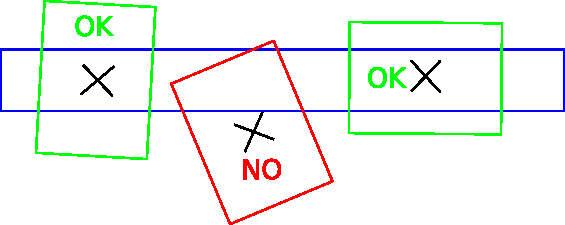
\includegraphics[width=0.9\linewidth]{contact1.pdf}
    \end{minipage}
    &
    %\begin{minipage}[t]{5cm}
    The center point of $S_1$ is included
    in $S_2$~\cite{hauser:humanoid:2005}
    \begin{itemize}
      \item Easy and cheap to compute
      \item Eliminates valid solutions
    \end{itemize}
    %\end{minipage}
    \\ \midrule
    \begin{minipage}{.4\textwidth}
      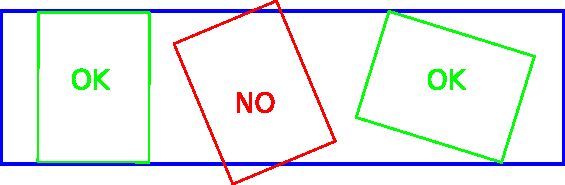
\includegraphics[width=0.8\linewidth]{contact2.pdf}
    \end{minipage}
    &
    %\begin{minipage}[t]{5cm}
    $S_1$ is fully included in $S_2$~\cite{bouyarmane:ar:2012}
    \begin{itemize}
      \item Eliminates many valid solutions
    \end{itemize}
    %\end{minipage}
    \\ \midrule
    \begin{minipage}{.4\textwidth}
      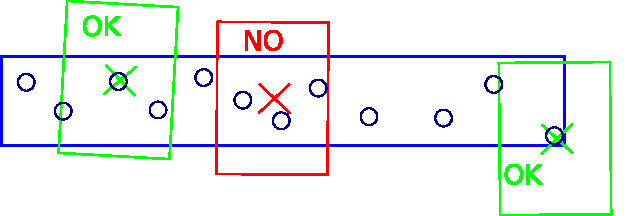
\includegraphics[width=\linewidth]{contact3.pdf}
    \end{minipage}
    &
    %\begin{minipage}[t]{5cm}
    $S_1$ contains a set of sampled points, the center of $S_2$ has to match one of them~\cite{chestnutt:humanoids:2003}
    \begin{itemize}
      \item Discrete set of possible solutions
      \item Eliminates many valid solutions
    \end{itemize}
    %\end{minipage}
    \\ \midrule
    \begin{minipage}{.4\textwidth}
      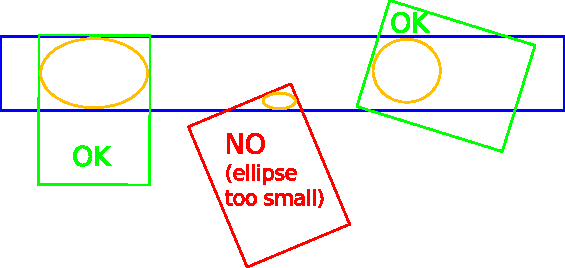
\includegraphics[width=0.9\linewidth]{contact4.pdf}
    \end{minipage}
    &
    %\begin{minipage}[t]{5cm}
    The contact is valid if an ellipse of sufficient size is found in
    the intersection $S_1 \cap S_2$~\cite{brossette:iros:2014}
    \begin{itemize}
      \item Smooth
      \item Does not eliminate valid solutions
    \end{itemize}
    %\end{minipage}
    \\ \bottomrule
  \end{tabular}
  \caption{Contact descriptions}
\label{tbl:contact_description}
\end{table}

In planning, once a geometric contact is found for a posture, the next posture will make use of it as a stability contact and apply forces on it.
Once the geometric contact is established, one determines the intersection of the contacting surfaces in order to find the points on which the reaction forces are to be computed when the geometric contact becomes a stability contact.
Several approaches require fixing the number of contact points or to have inclusive contact (i.e.\ one patch is fully included in the other)~\cite{bouyarmane:ar:2012}.

We provide a simple solution that relaxes contact constraints and gets rid of predefining the contact points.
We consider that a contact is valid if the intersection between two distinct patches has an area greater than a given threshold.
To enforce this, we require this intersection to contain an ellipse whose surface can possibly be maximized.
Convex patches allow writing the inscription constraints easily by means of half-spaces.


\subsection{Contact geometry formulation}
\label{subsec:contact_geometry_formulation}

%%%%%%%%%%%%%%%%%%%%%%%%%%%%%%%%%%%%%%%%%%%%%%%%%%%%%%%%%%%%%%%%%%%%%%%
%              SUBSECTION CONTACT GEOMETRY FORMULATION                %
%%%%%%%%%%%%%%%%%%%%%%%%%%%%%%%%%%%%%%%%%%%%%%%%%%%%%%%%%%%%%%%%%%%%%%%

%For our formulation, we consider a situation where a set of contacts between the robot and its environment are already made, and therefore fixed, and we want to add a new contact to this set.
%This doesn't induce any loss of generality since it just comes down to adding the contacts one by one.
%To ensure that the new contact can be reached in a quasi-static way, we look for a configuration where the new contact is a geometric contact.
%Let us consider that the contact to add is defined by two flat surfaces $S_1$ and $S_2$ which are respectively delimited by two convex polygons $P_1$ and $P_2$.
Let us consider a contact defined by two flat surfaces $S_1$ and $S_2$ which are respectively two convex polygons $P_1$ and $P_2$.
For this contact to be valid, it is necessary that the intersection $P_1 \cap P_2$ is not empty.
%We propose a method in which the size of the contact area is approximated by the size of an ellipse that is inscribed in it.
%If such an ellipse is found and is of a sufficient size, then the contact is valid.
%This allows considering contacts between surfaces that do not necessarily include each other.

An important remark is that the number of sides of the intersection polygon is not known a priori and, as shown in~\Figref{fig:polygon-inter}{}, this number can change depending on the configuration.
Each time this number changes, the gradient of the area of the intersection is discontinuous.
This is an issue for integrating any constraint or objective based on the area because we use a solver for smooth optimization problems.
This issue could be dealt with by using non-smooth optimization algorithms, but such algorithms are slower and less available, and our posture generator is not designed to use them.
\begin{figure}[!htb]
  \centering
  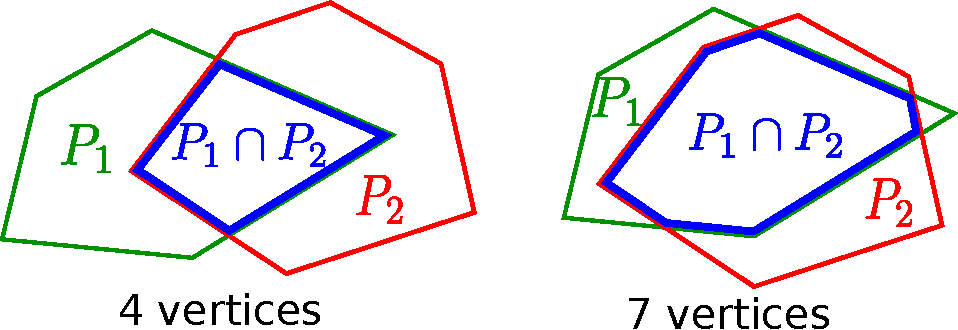
\includegraphics[width=0.6\columnwidth]{polygon-inter.pdf}
  \caption{Topological instability of $P_1 \cap P_2$}
\label{fig:polygon-inter}
\end{figure}
Moreover, supposing that we want to write constraints based on the sides of the contact area, then, the number of constraints would change with the number of vertex of $P_1 \cap P_2$.
The large majority of the optimization software cannot deal with a non-constant number of constraints.
The solution proposed in Section~\ref{subsec:ellipse} overcomes these issues by defining a set of constraints that is independent of the topology of the intersection area.



\subsection{Non-inclusive contact constraints}
\label{subsec:ellipse}

%%%%%%%%%%%%%%%%%%%%%%%%%%%%%%%%%%%%%%%%%%%%%%%%%%%%%%%%%%%%%%%%%%%%%%%
%          SUBSECTION NON-INCLUSIVE CONTACT CONSTRAINTS               %
%%%%%%%%%%%%%%%%%%%%%%%%%%%%%%%%%%%%%%%%%%%%%%%%%%%%%%%%%%%%%%%%%%%%%%%



\subsubsection{Main Idea}
\label{subsubsec:idea}

%%%%%%%%%%%%%%%%%%%%%%%%%%%%%%%%%%%%%%%%%%%%%%%%%%%%%%%%%%%%%%%%%%%%%%%
%                      SUBSUBSECTION MAIN IDEA                        %
%%%%%%%%%%%%%%%%%%%%%%%%%%%%%%%%%%%%%%%%%%%%%%%%%%%%%%%%%%%%%%%%%%%%%%%

We propose a smooth formulation of the non-empty intersection between two contact surfaces.
We assume that co-planarity of $S_1$ and $S_2$ is obtained by using the constraints presented in~\Eqref{eq:coplanarity}.
Here we focus on the intersection of the two polygons $P_1$ and $P_2$, respectively describing the contours of $S_1$ and $S_2$.
%As we pointed out earlier, a problem with computing the area of intersection of two polygons comes from the fact that depending on their positions in space, the number of edges of their intersection can change (cf.~\Figref{fig:polygon-inter}{}), which induces discontinuity of the gradient of the area and change of the number of constraints associated with this contact.

To avoid dealing with changes of topology, we consider using an ellipse $\mathcal{E}$ included in $P_1 \cap P_2$ to estimate the area of the intersection.
Since $P_1$ and $P_2$ are convex polygons, then $P_1 \cap P_2$ is also a convex polygon.
A convex polygon can be seen as an intersection of half-planes based on the lines supporting its edges.
Thus, an ellipse is inside of a convex polygon if it lies entirely in the corresponding half-planes.
Having the ellipse be included in the intersection of two polygons is equivalent to having it included in both polygons:
\begin{equation}
\mathcal{E} \subset P_1 \cap P_2 \ \Longleftrightarrow \
\mathcal{E} \subset P_1 \ \ \text{AND} \ \  \mathcal{E} \subset P_2
\end{equation}
Even if the number of edges of $P_1 \cap P_2$ can change, the numbers of edges of $P_1$ and $P_2$ respectively are fixed.
%\begin{wrapfigure}{r}{0.4\columnwidth}
%  \begin{center}
%    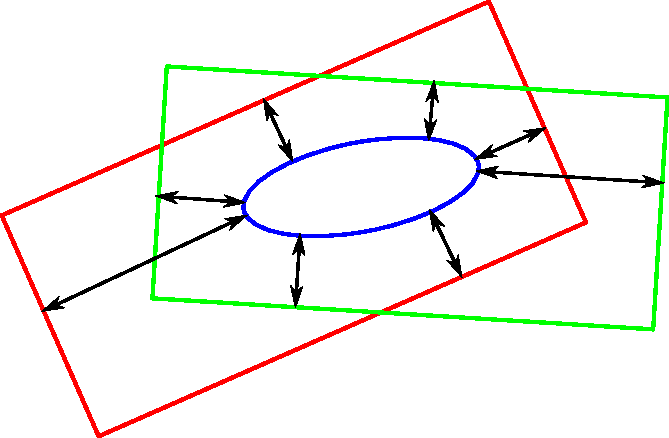
\includegraphics[width=0.4\columnwidth]{distance.pdf}
%    \caption{Distance ellipse-polygons}
%  \end{center}
%  \label{fig:distance}
%\end{wrapfigure}
%Therefore, if we ensure that the ellipse $\mathcal{E}$ is on the left side of each segment defining $P_1$ and $P_2$, then it is inside $P_1 \cap P_2$.
To assert that an ellipse lies in a half-plane, we need a function that is positive when the ellipse is in it (with zero value when the ellipse is on the edge) and negative otherwise.
The signed distance to the line defining the half-space is a good candidate (distance ellipse-line if the ellipse is in the half-plane, opposite of the penetration distance if not), but actually, any pseudo-distance does the job.
And a sufficient condition for the ellipse to be inside the polygons intersection is that the pseudo-distance between the ellipse and each edge of both polygons is positive (see~\Figref{fig:distance}{}).
By considering each edge separately as opposed to the pseudo-distance of the ellipse to a whole polygon, we can write smooth constraints with a simple pseudo-distance function.
We develop such a pseudo-distance in what follows.
%In order to measure the fact that a point is on the left side of an oriented segment we use a signed distance $d_s$, this signed distance is positive and equal to a usual distance when the point is on the left side of the segment and is negative and equal to the opposite of the usual distance when the point is on the right side of the segment.
% and algorithm~\ref{alg:ellipse-in-intersection} where $d_s$ stand for the pseudo-distance.
%\begin {algorithm}
%\caption{Inclusion of ellipse $\mathcal{E}$ in polygon intersection}
%\begin{algorithmic}
%\STATE {Let $P_1$ and $P_2$ be two coplanar convex polygons}
%\STATE {Let {\bf V} be an empty vector}
%\FORALL{Edge E in $P_1$}
%\STATE {Add $d_s(\mathcal{E}, E)$ to {\bf V}}
%\ENDFOR
%\FORALL{Edge E in $P_2$}
%\STATE {Add $d_s(\mathcal{E}, E)$ to {\bf V}}
%\ENDFOR
%\IF {{\bf V}$\succ 0$ (all terms of {\bf V} are positive)}
%\STATE {Return $\mathcal{E} \subset P_1 \cap P_2$}
%\ELSE
%\STATE {Return $\mathcal{E} \not\subset P_1 \cap P_2$}
%\ENDIF
%\end{algorithmic}
%\label{alg:ellipse-in-intersection}
%\end{algorithm}
%
\begin{figure}[!htb]
  \centering
  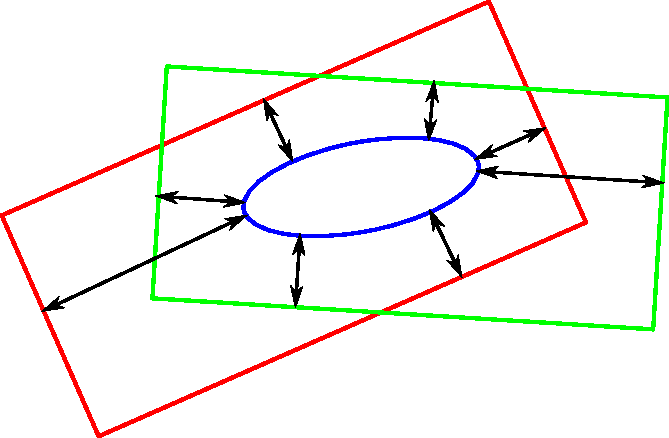
\includegraphics[width=0.4\columnwidth]{distance.pdf}
  \caption{Distance between $\mathcal{E}$ and $P_1 \cap P_2$.}
\label{fig:distance}
\end{figure}

\subsubsection{Pseudo-distance}
\label{subsubsec:formulation}

%%%%%%%%%%%%%%%%%%%%%%%%%%%%%%%%%%%%%%%%%%%%%%%%%%%%%%%%%%%%%%%%%%%%%%%
%                   SUBSUBSECTION PSEUDO-DISTANCE                     %
%%%%%%%%%%%%%%%%%%%%%%%%%%%%%%%%%%%%%%%%%%%%%%%%%%%%%%%%%%%%%%%%%%%%%%%

%To estimate the constraint of inclusion of the ellipse $\mathcal{E}$ in both polygons $P_1$ and $P_2$, we need to compute the signed distance between $\mathcal{E}$ and each segment of the polygons.
Computing the distance between an ellipse and a line is not straightforward, whereas the distance between a line and a circle is very easy to compute.
Also, we note that in the frame $F_\mathcal{E}$ defined by the ellipse's axes and pseudo-radius, the ellipse is a circle of radius $r_{\mathcal{E}}=1$ (The x-unit along the first axis of the ellipse is $r_x$, the first radius of the ellipse, the y-unit along the second axis of the ellipse is $r_y$, the second radius).
The transformation from the original frame $F_0$ in which the ellipse and the polygons are described to the ellipse's frame $F_\mathcal{E}$ is just the composition of a rotation and a scaling of the space along the axes of the ellipse with a scaling vector $[\frac{1}{r_x}, \frac{1}{r_y}]$.
The effect of such a transformation applied to an ellipse and two polygons is shown in~\Figref{fig:pseudo-distance}{}.
%Also, those transformations will not modify the validity of our constraint, indeed, the distance between $\mathcal{E}$ and any segment $E$, computed in $F_\mathcal{E}$, is a pseudo-distance in $F_0$.
%Therefore, we still get all the information needed to ensure the inclusion of $\mathcal{E}$ in $P_1 \cap P_2$.
We thus defined the following pseudo-distance from an ellipse to a half-plane as the signed Euclidean distance from the corresponding unit circle to the transformed half-plane in the frame $F_\mathcal{E}$.

\begin{figure}[!htb]
  \centering
  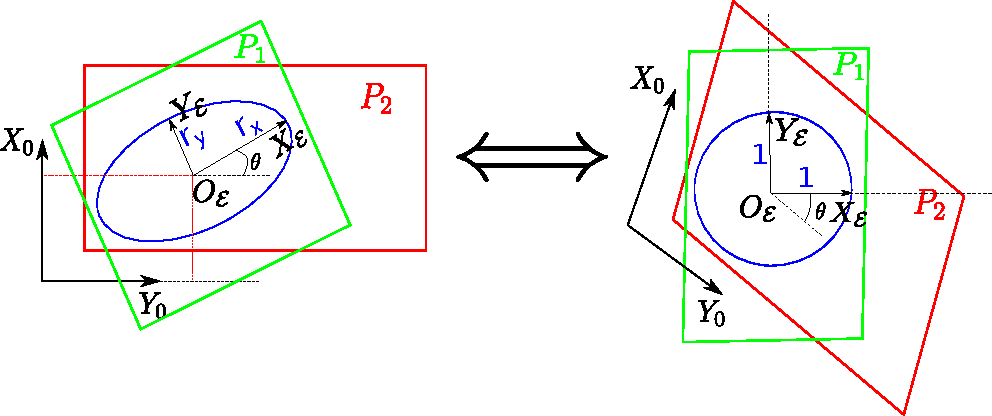
\includegraphics[width=0.9\linewidth]{pseudo-distance.pdf}
  \caption{Transformation from $F_0(O_0, X_0, Y_0)$ to $F_\mathcal{E}(O_\mathcal{E},X_\mathcal{E},Y_\mathcal{E})$}
\label{fig:pseudo-distance}
\end{figure}

Now let us consider a single segment $p_i p_j$ and an ellipse $\mathcal{E}$ defined in $F_0$.
The expression of a vector ${{\bf v}_{F_0}}^T = {[v_x, v_y]}_{F_0}$ in $F_\mathcal{E}$ is obtained by applying the formula~\Eqref{eq:F0-to-FE}.
\begin{equation}
{\bf v}_{F_\mathcal{E}} =
\begin{bmatrix}
\frac{1}{r_x} & 0 \\
0 & \frac{1}{r_y}
\end{bmatrix}
\cdot \begin{bmatrix}
\cos(\theta) & \sin(\theta) \\
-\sin(\theta) & \cos(\theta)
\end{bmatrix}
\cdot {\bf v}_{F_0}
\label{eq:F0-to-FE}
\end{equation}
In $F_\mathcal{E}$, the distance between the circumference of $\mathcal{E}$ and the segment $p_i p_j$ is:
\begin{equation}
  d_s(\mathcal{E}, p_i p_j) = \frac{{\left.\overrightarrow{p_i p_j}\right|}_{F_\mathcal{E}} \wedge {\left.\overrightarrow{p_i O_\mathcal{E}}\right|}_{F_\mathcal{E} } }{\| \overrightarrow{p_i p_j}\|_{F_\mathcal{E} } }-1
\end{equation}
where $\wedge$ denotes the cross product and $O_{\mathcal{E}}$ is the center of the ellipse.

To avoid numerical problems when the segment $p_i p_j$ is small, it is preferable to multiply this distance by $\| \overrightarrow{p_i p_j}\|_{F_\mathcal{E}}$ before using it as a constraint.
Then we get the following constraint:
\begin{equation}
  -{\left.\overrightarrow{p_i p_j}\right|}_{F_\mathcal{E}} \wedge {\left.\overrightarrow{p_i O_\mathcal{E}}\right|}_{F_\mathcal{E}}+\| \overrightarrow{p_i p_j}\|_{F_\mathcal{E}} \leq 0
\label{eq:pseudo-distance}
\end{equation}

The combination of these equations~\Eqref{eq:F0-to-FE} and \Eqref{eq:pseudo-distance} applied for each edge of the polygons gives us all the necessary tools to develop a set of constraints that ensures that an ellipse is inside the intersection of two polygons.



\subsubsection{Modification of the optimization problem}

%%%%%%%%%%%%%%%%%%%%%%%%%%%%%%%%%%%%%%%%%%%%%%%%%%%%%%%%%%%%%%%%%%%%%%%
%       SUBSUBSECTION MODIFICATION OF THE OPTIMIZATION PROBLEM        %
%%%%%%%%%%%%%%%%%%%%%%%%%%%%%%%%%%%%%%%%%%%%%%%%%%%%%%%%%%%%%%%%%%%%%%%

To include the above idea in our posture generation, we need to modify the optimization problem~\Eqref{eq:PG} as follows.
Each non-inclusive geometrical contact adds five variables to the optimization vector, corresponding to the position, orientation, and radiuses of the ellipse ($x$, $y$, $\theta$, $r_x$ and $r_y$).
One constraint of ellipse inclusion (as described above) is added to the problem for each edge of the polygons.
The parameters $r_x$ and $r_y$ are given lower positive bounds to ensure that the ellipse is not empty.
The existence of a contact between $S_1$ and $S_2$ is thus transformed into the existence of $r_x$ and $r_y$ respecting their bounds.
In summary, this kind of constraint adds 5 variables and $card(P_1)+card(P_2)$ constraints to the optimization problem (where $card(P)$ denotes the number of edges of polygon $P$), while the `usual' inclusion constraint adds 0 variable and $card(P_1)card(P_2)$ constraints.
The existence of the contact can alternatively be enforced by imposing a minimum area for the ellipse.



\subsubsection{Maximization of the contact area}
\label{subsubsec:optim-ellipse-area}

%%%%%%%%%%%%%%%%%%%%%%%%%%%%%%%%%%%%%%%%%%%%%%%%%%%%%%%%%%%%%%%%%%%%%%%
%           SUBSUBSECTION MAXIMIZATION OF THE CONTACT AREA            %
%%%%%%%%%%%%%%%%%%%%%%%%%%%%%%%%%%%%%%%%%%%%%%%%%%%%%%%%%%%%%%%%%%%%%%%

The formulation in the above section only ensures the existence of a contact of minimal size.
However, one may want to find a contact area as large as possible, so that it is more likely to be able to support strong forces and have strong friction forces, which is helpful to guarantee the stability of the robot.
Therefore, it seems appropriate to try and maximize the area of contact between two polygons.
As explained before, computing the area of the intersection surface is not a good practice in our case.
But the ellipse computed as above gives a lower bound of the contact area.

\begin{equation}
\mathcal{E} \subset P_1 \cap P_2 \Longrightarrow  \mathcal{A}(\mathcal{E}) \le \mathcal{A}(P_1 \cap P_2)
\end{equation}
with $\mathcal{A}(X)$ being the area of $X$.\newline
Therefore, we can maximize the area of the ellipse in order to maximize the contact area.
This is readily obtained by minimizing the value of $f_{\text{ellipse}}(r_x, r_y) = -\pi r_x r_y$ in the modified problem~\Eqref{eq:PG}.
In case there are other cost functions, the above cost can be added to them with a desired weight.
This requires, however, to scale properly the cost so as to have a meaningful and easy-to-tune weight: the range of value of the ellipse's area goes from $0$ to $\mathcal{A}(P_1 \cap P_2) \leq \min (\mathcal{A}(P_1), \mathcal{A}(P_2))$.
This latter quantity can be small (a typical area of contact of a humanoid robot is about $0.01m^2$, some environment surfaces can be smaller).
To get a basic cost (before weighting) of magnitude around $1$, we use the following scaling:
\begin{equation}
f_\text{ellipse}(r_x, r_y) = - \frac{\pi r_x r_y}{\min (\mathcal{A}(P_1), \mathcal{A}(P_2))}
\label{eq:cost-ellipse}
\end{equation}
This cost's absolute value will always be less than $1$, but not much less around the optimum, in most cases.


\subsubsection{Using a non-inclusive contact to maintain stability}
\label{subsubsec:stability}

%%%%%%%%%%%%%%%%%%%%%%%%%%%%%%%%%%%%%%%%%%%%%%%%%%%%%%%%%%%%%%%%%%%%%%%
%  SUBSUBSECTION USING A NON-INCLUSIVE CONTACT TO MAINTAIN STABILITY  %
%%%%%%%%%%%%%%%%%%%%%%%%%%%%%%%%%%%%%%%%%%%%%%%%%%%%%%%%%%%%%%%%%%%%%%%

The method we presented so far allows finding a configuration in which a new non-inclusive contact is added, but this contact does not bear any force.
It is found as a geometrical contact, but will eventually have to bear some forces, and thus, become a stability contact.
Usually, for a stability contact, each vertex of the contact area is considered as the application point of a force that has to be in a friction cone.
Since our method allows dealing with surfaces that are intersecting each other, the contact surface is not known beforehand.
Therefore, as soon as a non-inclusive contact is going to be used for the stability, we compute the intersection of the two polygons $P_1$ and $P_2$ that are involved, and that intersection $P_1 \cap P_2$ is the contact surface, and its vertices will bear the forces.
We do not present here the algorithm to compute the intersection of two convex polygons, as it can be found in the literature easily.
%Since this computation is done outside of the posture generation, it does not imply any numerical problems.

\subsubsection{Extension to singular cases}
\label{subsubsec:singular_cases}
Our method can be extended to be used to approximate singular situations, such as finding an optimal contact with a linear or even punctual surface.
This is done by giving a slight width to the point or the line.
This approximation is physically grounded:
%The main problem with that kind of approach is that it is not possible to deal with a perfectly linear surface, that's why we call "line" a very thin rectangle and "point" a very small square.
in terms of real contacts, linear or punctual contacts do not exist.
In fact, since all objects are deformable, even slightly, the contact area between two objects cannot be a perfect line, and must have a non-null area, which justifies that linear and punctual contacts can be modeled as thin contact surfaces.
By defining such a surface, we impose partly the orientation of the contact.
%A problem we encountered with that extension is that if the contact area is thin, then the ellipse  found inside this area will be thin too and thus have a small area.
%This lead to some conditioning problems and at first the solver would stop without optimizing the size of the ellipse.
%That was due to the fact that the area of the ellipse was negligible compared to the other costs involved in the cost function.
%That is why we divided the area of the ellipse by $\min (\mathcal{A}(P_1), \mathcal{A}(P_2))$ to get the equation~\Eqref{eq:cost-ellipse} in the first place.
Here again, one must be careful with numerical issues.
Dealing with small numbers (here we would like to take the width of a fraction of a centimeter) may induce conditioning problems.
Also, having two close parallel constraints of opposite direction (i.e. $g(x)\leq \alpha$ and  $-g(x)\leq \alpha$ with $\alpha$ small) is not a good practice in optimization as it will lead the solver to take small steps.
Therefore, it is best to apply a scaling to the constraints by applying a geometrical scaling to $P_1$ and $P_2$ in the appropriate direction.\newline
Likewise, constraints on the area of the ellipse should be based on the same formulation as in equation~\Eqref{eq:cost-ellipse}.



\subsection{Simulation results}
\label{subsec:simu}

%%%%%%%%%%%%%%%%%%%%%%%%%%%%%%%%%%%%%%%%%%%%%%%%%%%%%%%%%%%%%%%%%%%%%%%
%                   SUBSECTION SIMULATION RESULTS                     %
%%%%%%%%%%%%%%%%%%%%%%%%%%%%%%%%%%%%%%%%%%%%%%%%%%%%%%%%%%%%%%%%%%%%%%%

In order to illustrate our method, we present some examples starring the HRP-2 and ATLAS humanoid robots, that are typical posture generations encountered in multi-contact planning.
%All the computations of the following experiments are performed on a single thread of an Intel(R) Core(TM) i7-3840QM CPU at 2.80GHz, with 16Go of RAM.
For the implementation of our posture generator, we use the RobOptim optimization framework~\cite{moulard:jsme:2013} relying on the IPOPT solver~\cite{wachter:mathprog:2006}.



\subsubsection{Inclined ladder climbing}
\label{subsubsec:inclined_ladder_climbing}

%%%%%%%%%%%%%%%%%%%%%%%%%%%%%%%%%%%%%%%%%%%%%%%%%%%%%%%%%%%%%%%%%%%%%%%
%               SUBSUBSECTION INCLINED LADDER CLIMBING                %
%%%%%%%%%%%%%%%%%%%%%%%%%%%%%%%%%%%%%%%%%%%%%%%%%%%%%%%%%%%%%%%%%%%%%%%

In this first example, we generate a posture that is part of an inclined ladder climbing planning.
We consider that the robot HRP-2 reached a posture in which its right foot is on the first step and its right hand is grasping the right guardrail, both of those contacts are bearing forces.
Those contacts are fixed, and we search a posture that adds to it a geometrical contact between the left foot and the second step.
We require the contact to include an ellipse with both radiuses bigger than 40\% of the ladder step's width.
The resulting posture and a close-up view of the contact areas are shown in~\Figref{fig:hrp2_darpa_complete}{}.
The latter shows clearly how an ellipse of sufficient size is found, included in the contact area between the left foot and the second step.
It also shows that the contact forces on the right foot are located on the vertex of the intersection of the contact surfaces between the right foot and the first step, which was also generated with our method, in a prior posture generation.
One can note that we use a contact area slightly smaller than the actual surface under the foot of the robot.
We use indeed safety margins to account for modeling errors so that the obtained posture is achievable by the real robot.
%\begin{figure*}
%\centering
%\begin{subfigure}{.5\textwidth}
%  \centering
%  \setlength\fboxsep{0pt}
%  \setlength\fboxrule{1pt}
%  %\fbox{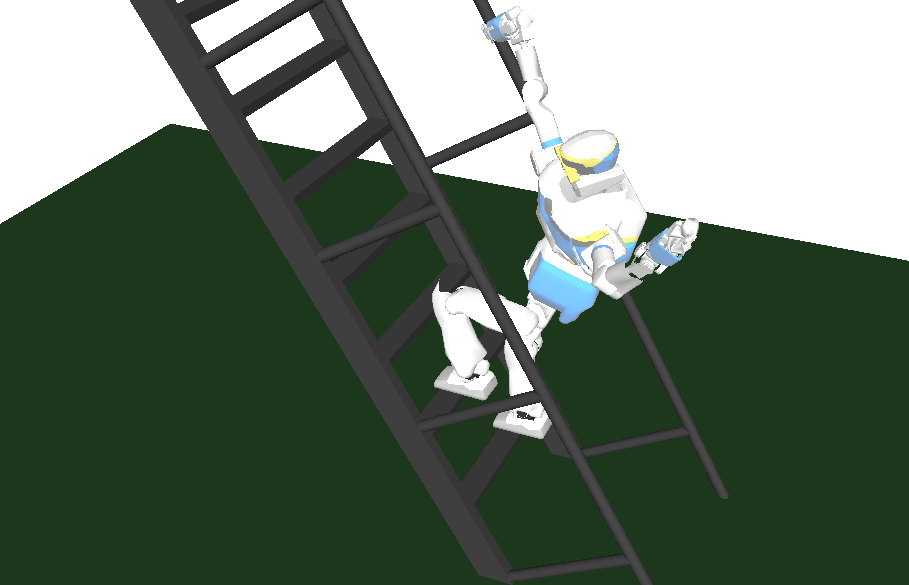
\includegraphics[width=\linewidth]{papers/IROS2014/figure/hrp2_ladder_darpa.png}}
%  %\fbox{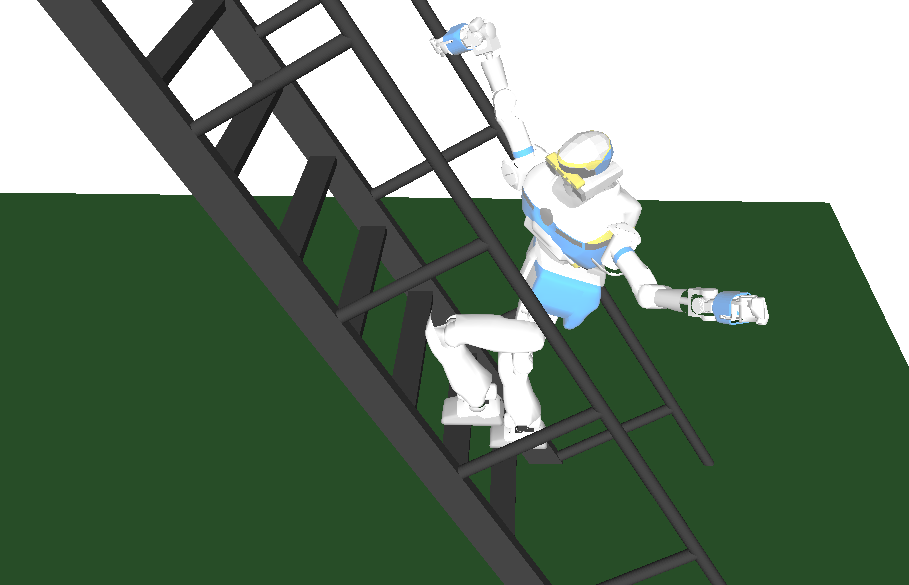
\includegraphics[width=\linewidth]{figure/hrp2_ladder_darpa_40.png}}
%  \fbox{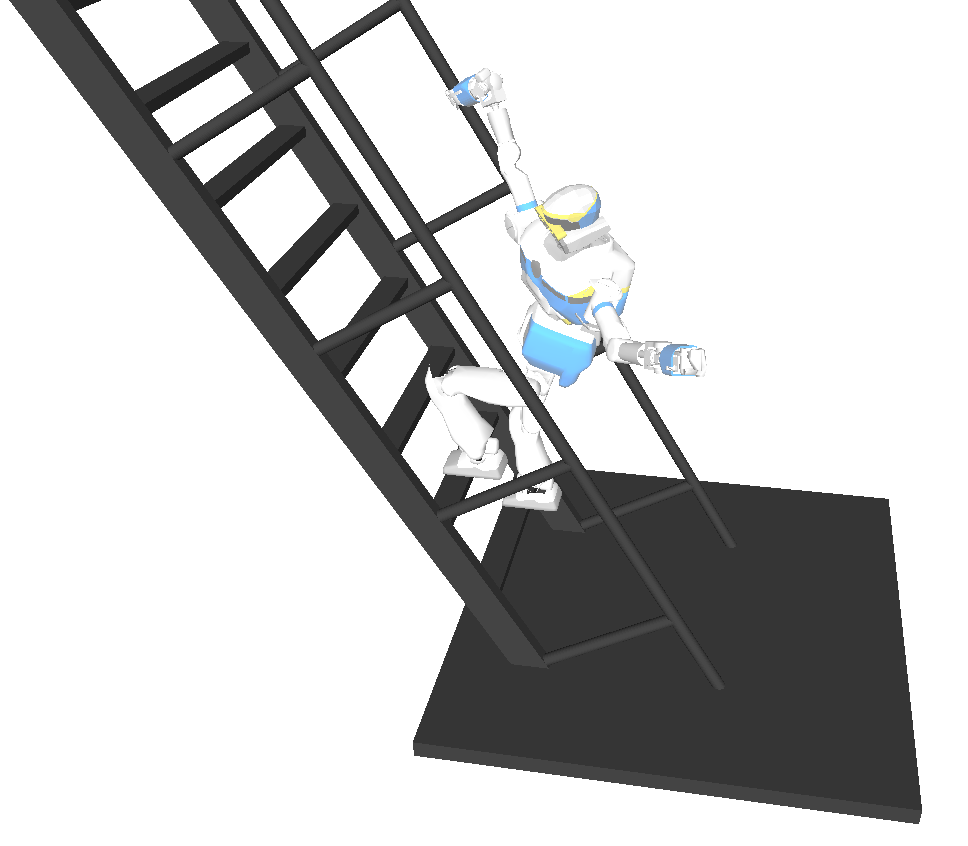
\includegraphics[width=\linewidth]{figure/hrp2_darpa_small.png}}
%  %\caption{HRP2-10 ladder climbing posture}
%  \label{fig:hrp2_darpa}
%\end{subfigure}%
%\begin{subfigure}{.5\textwidth}
%  \centering
%  \setlength\fboxsep{0pt}
%  \setlength\fboxrule{1pt}
%  %\fbox{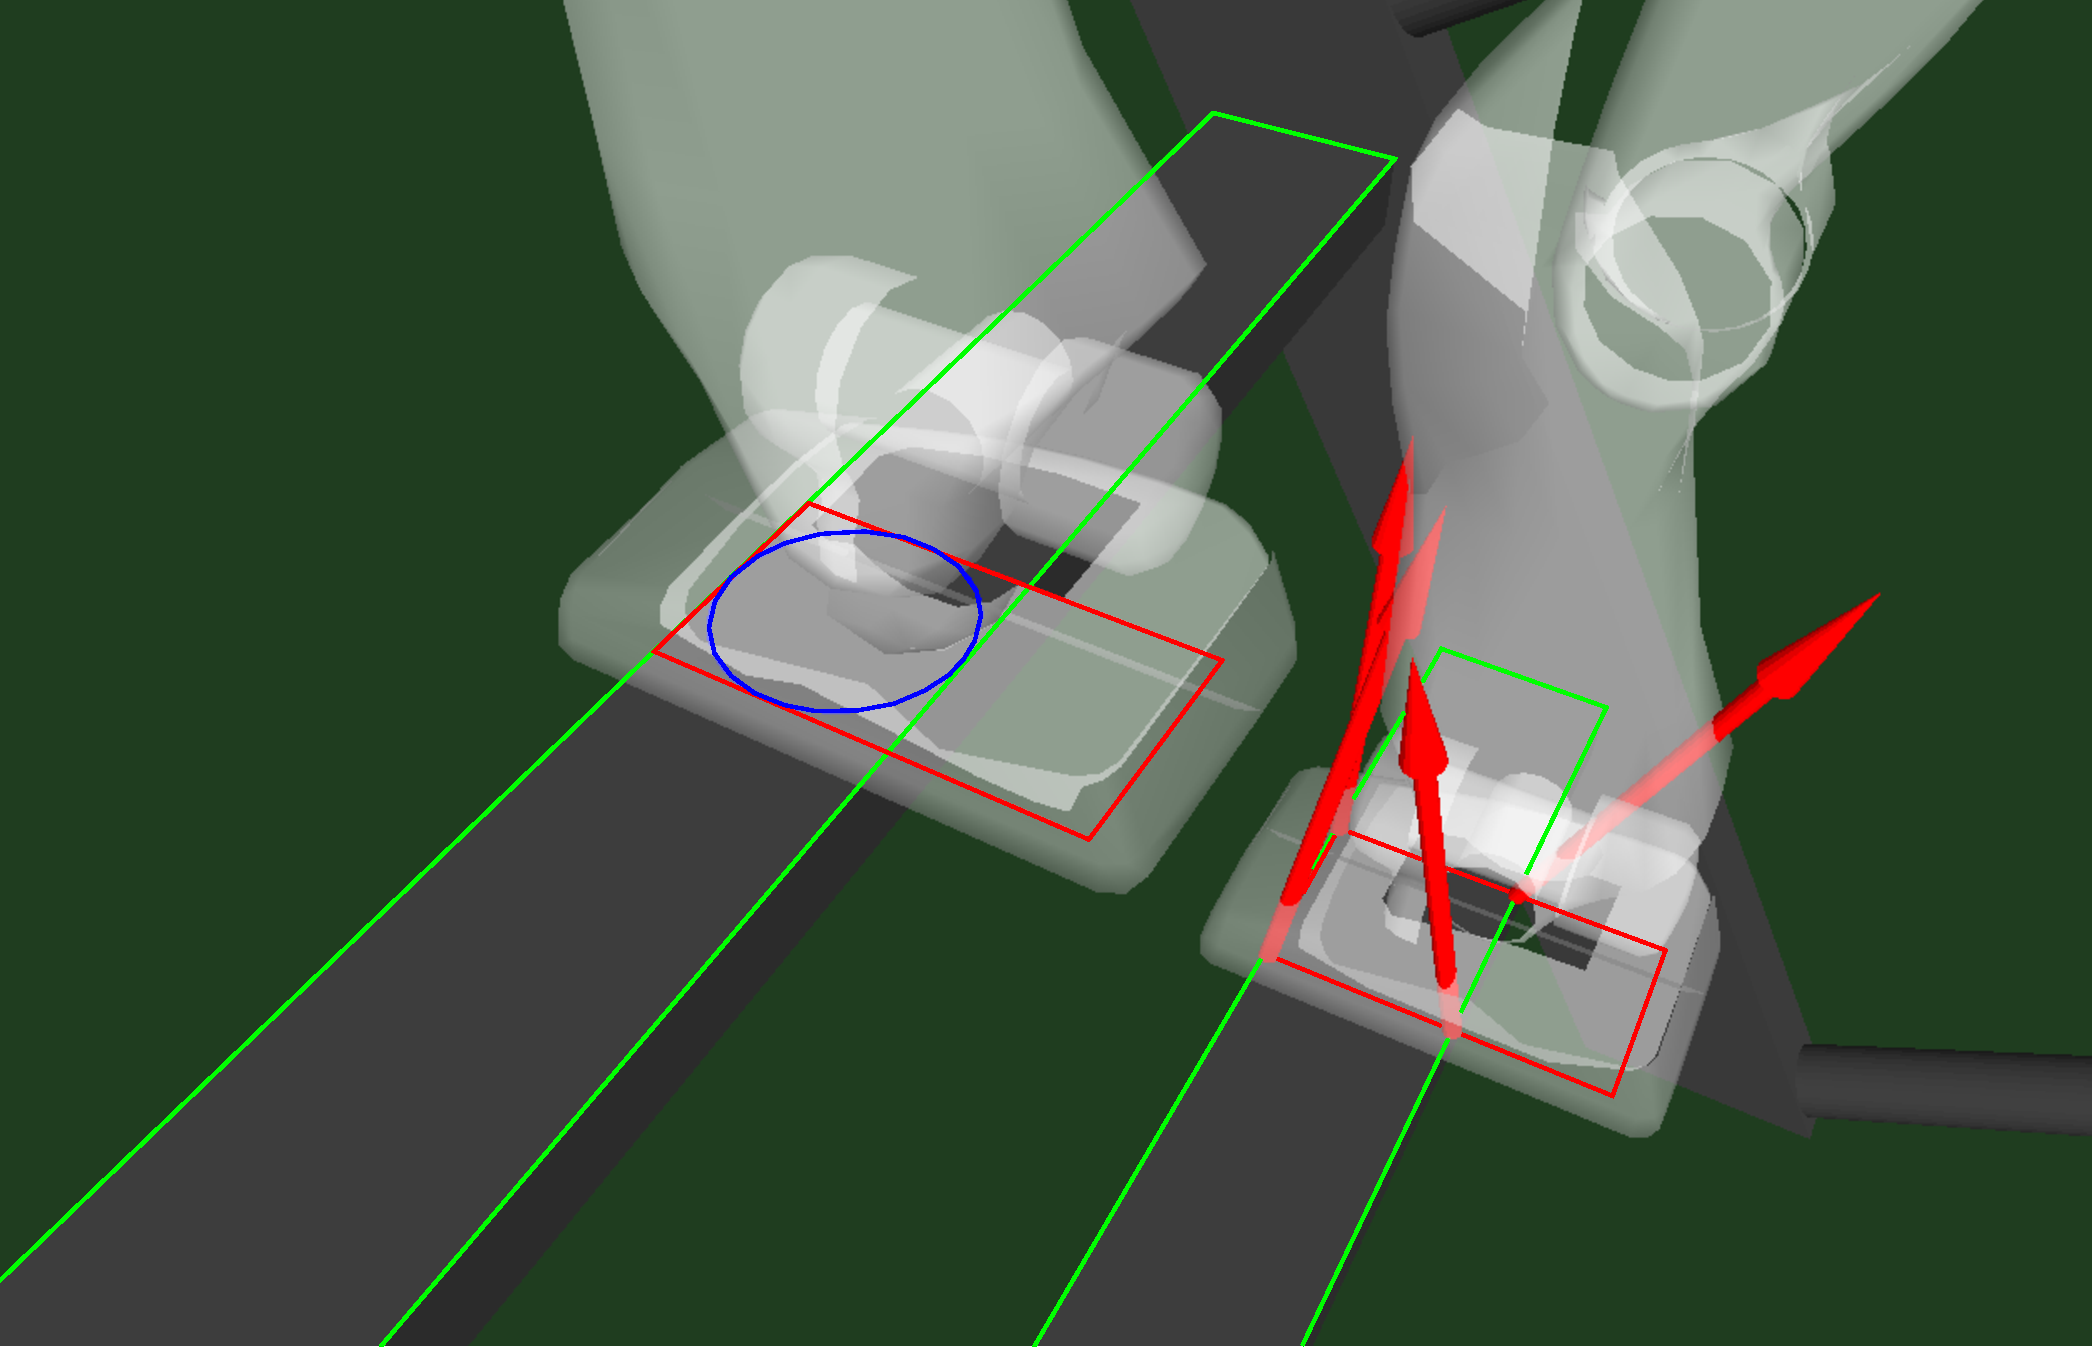
\includegraphics[width=\linewidth]{figure/hrp2_ladder_darpa_zoom.pdf}}
%  %\fbox{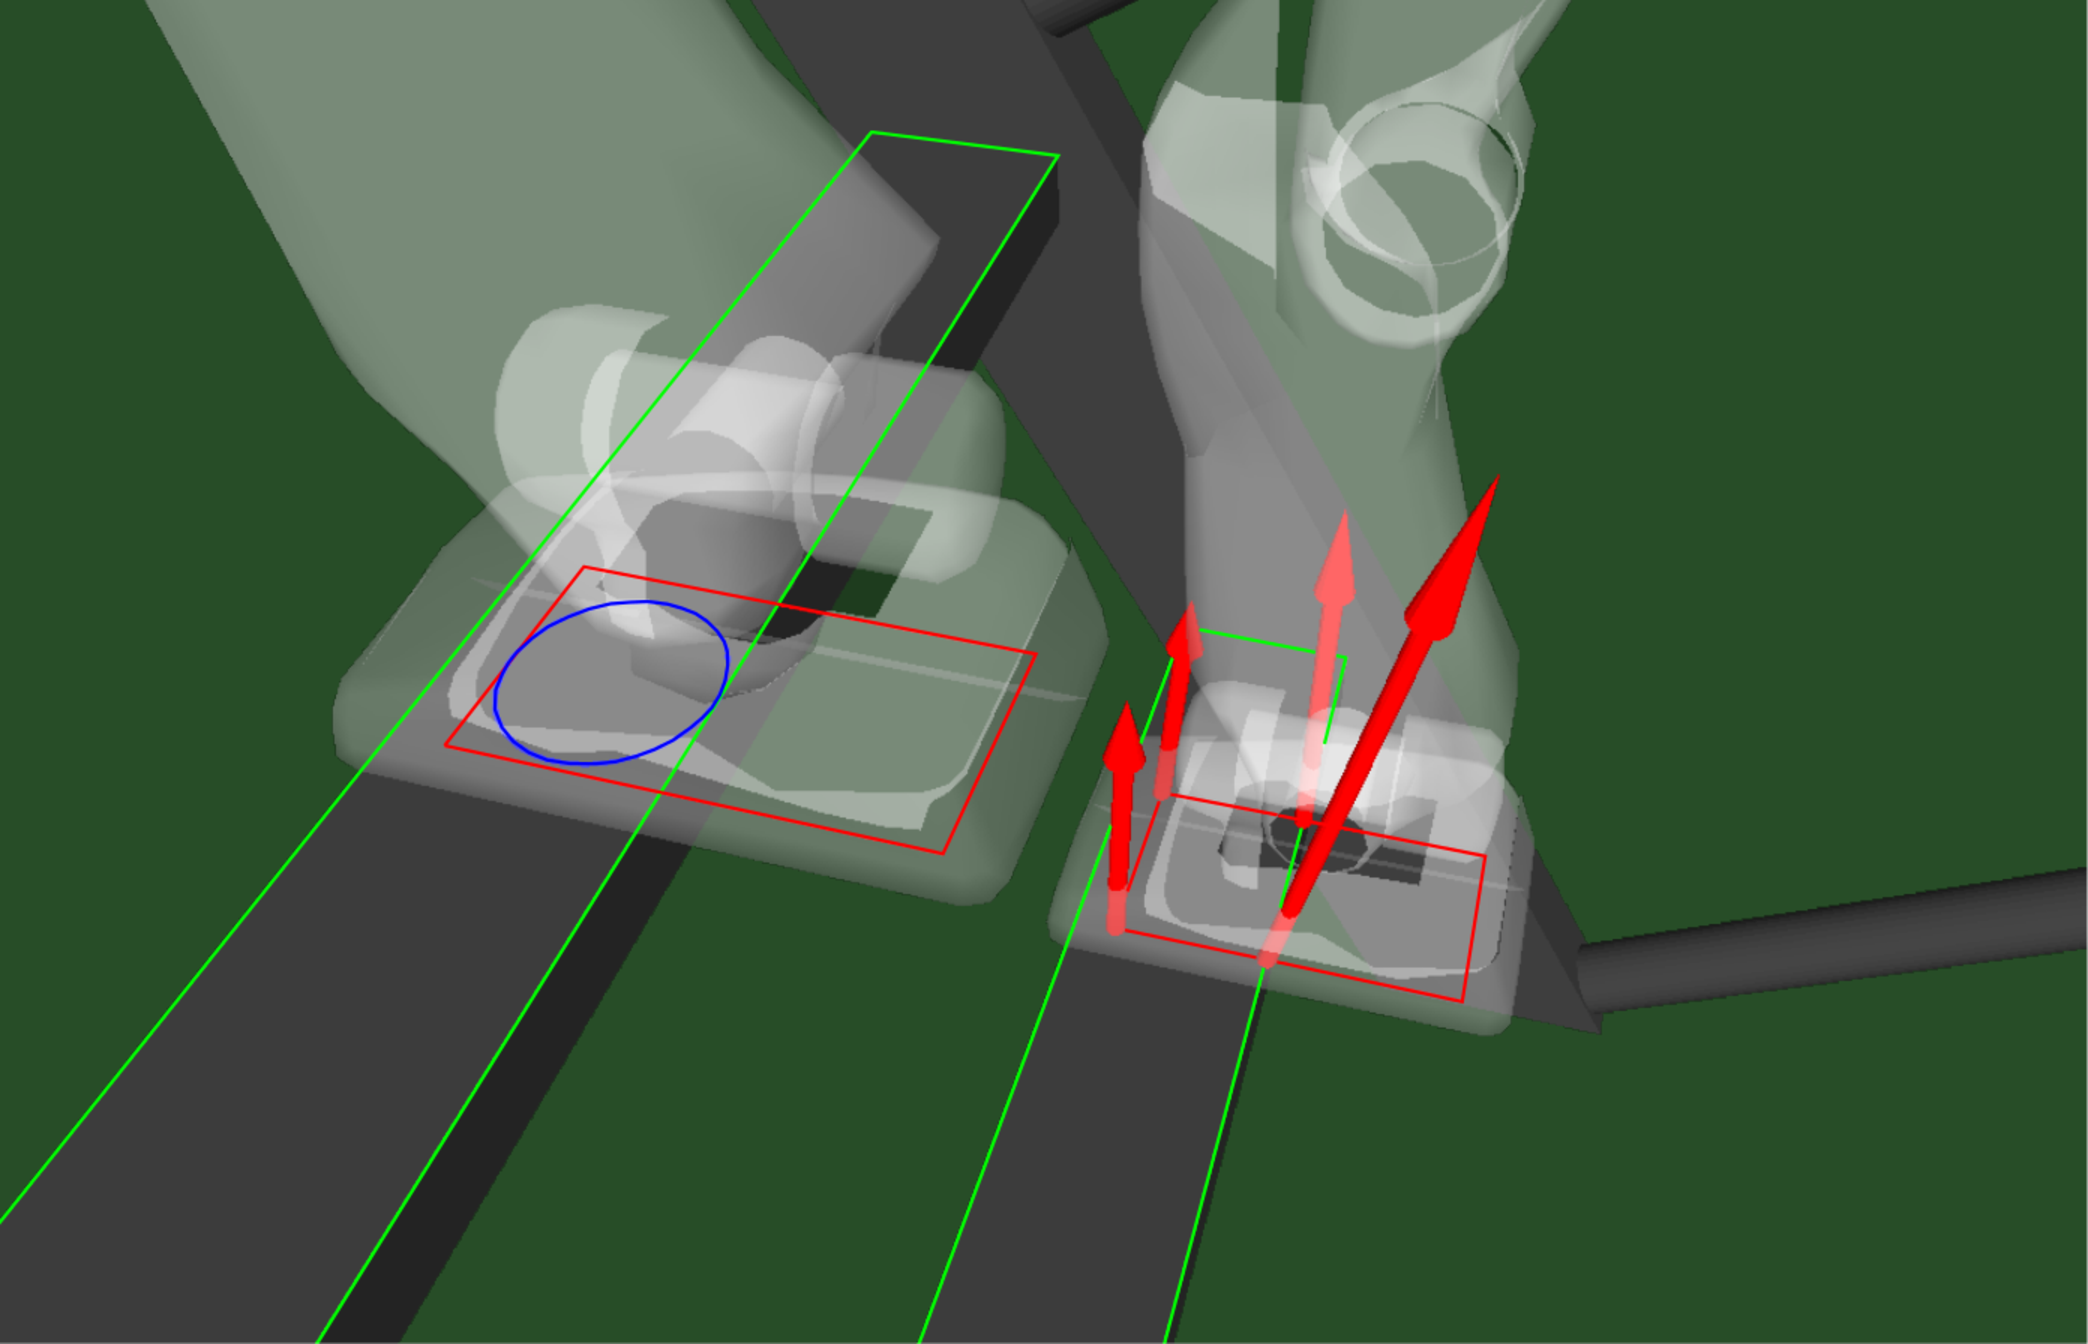
\includegraphics[width=\linewidth]{figure/hrp2_ladder_darpa_40_zoom.pdf}}
%  \fbox{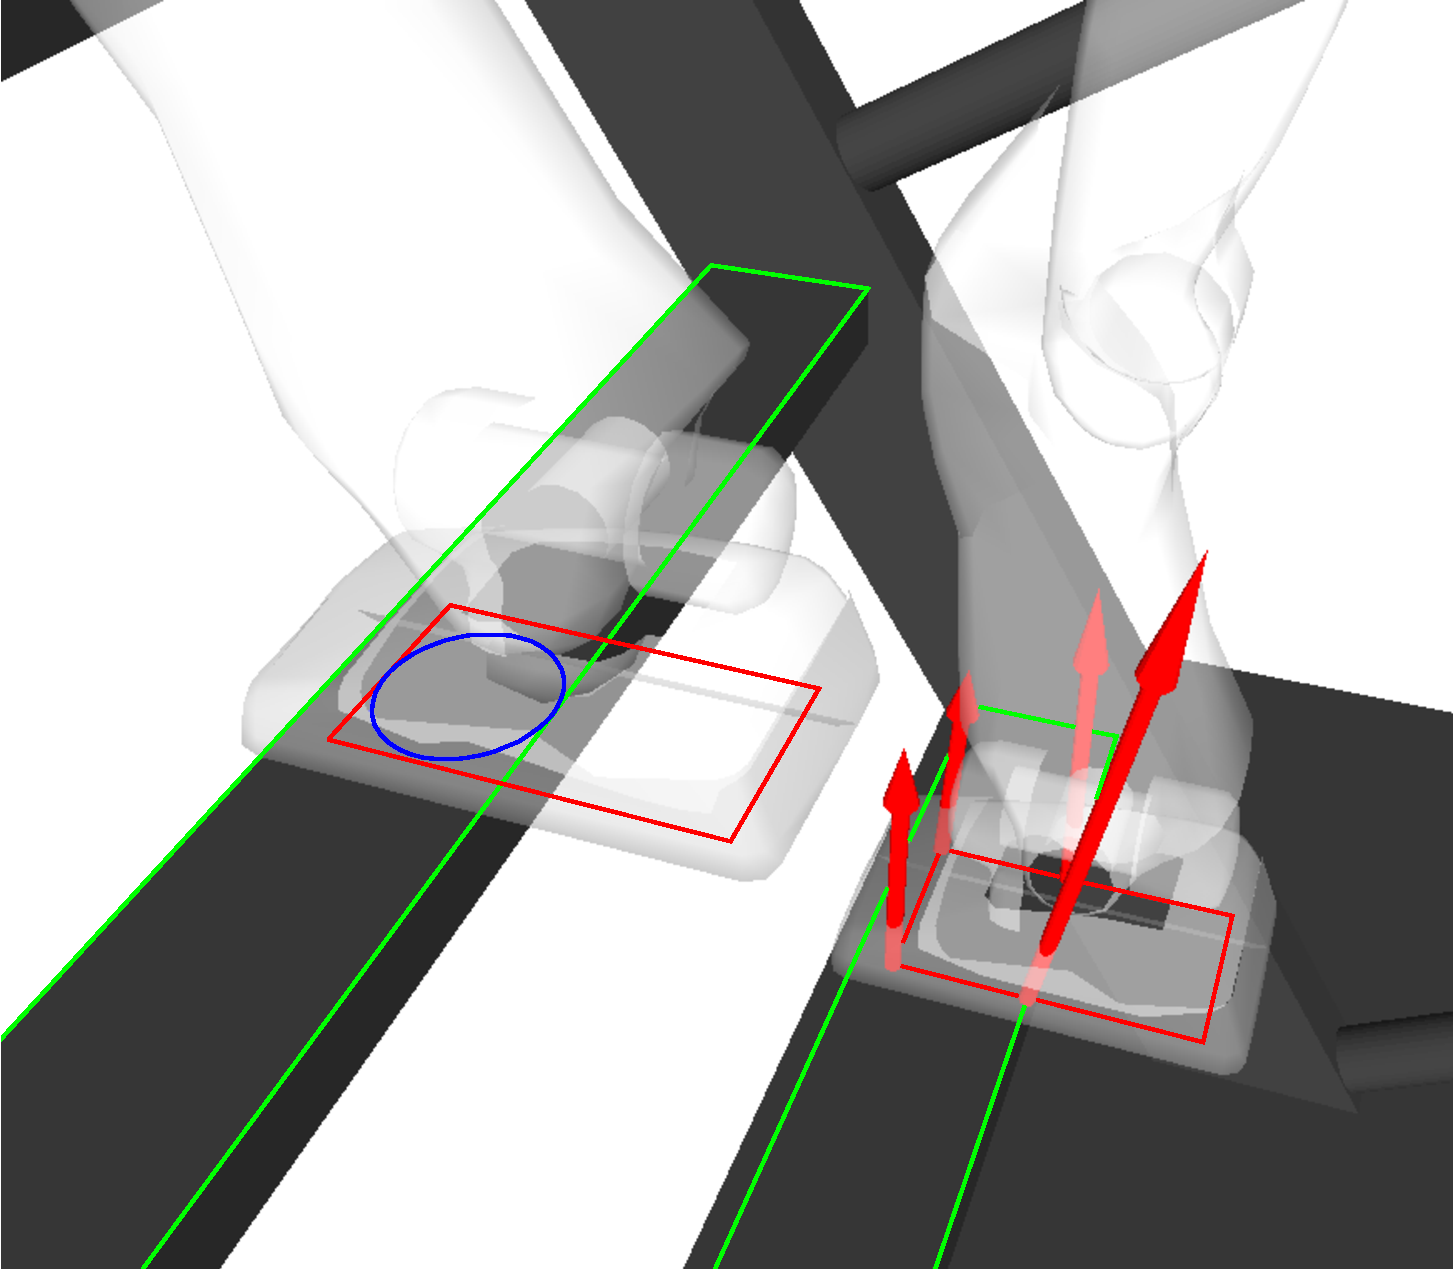
\includegraphics[width=\linewidth]{figure/hrp2_darpa_small_zoom.pdf}}
%  %\caption{Upclose view of the contact areas (green and red: contact polygon, blue: ellipse found in contact area, Red arrows: contact forces resultants)}
%  \label{fig:hrp2_darpa_zoom}
%\end{subfigure}
%\caption{(a)HRP2-10 ladder climbing posture; (b)Upclose view of the contact areas\\(green/red: contact polygons; blue: ellipse found in contact area; red arrows: contact forces resultants)}
%\label{fig:hrp2_darpa_complete}
%\end{figure*}

%\begin{figure}
%\centering
%\begin{subfigure}{.3325\columnwidth}
  %\centering
  %\setlength\fboxsep{0pt}
  %\setlength\fboxrule{1pt}
  %\fbox{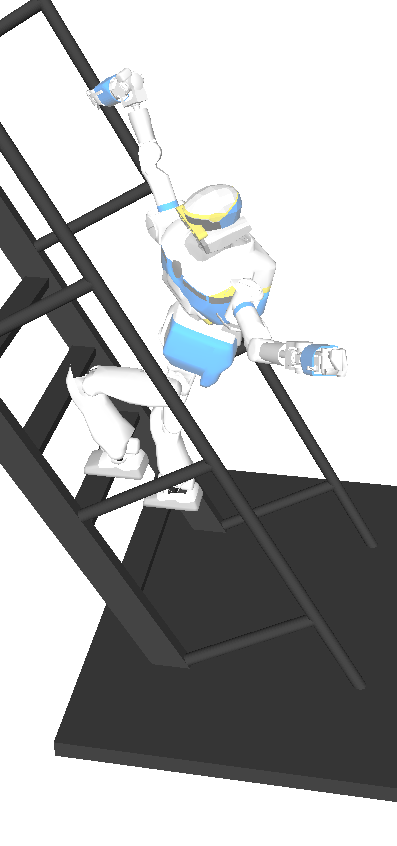
\includegraphics[width=0.95\linewidth]{hrp2_darpa_small_cut.png}}
%\label{fig:hrp2_darpa}
%\end{subfigure}%
%\begin{subfigure}{.6175\columnwidth}
  %\centering
  %\setlength\fboxsep{0pt}
  %\setlength\fboxrule{1pt}
  %\fbox{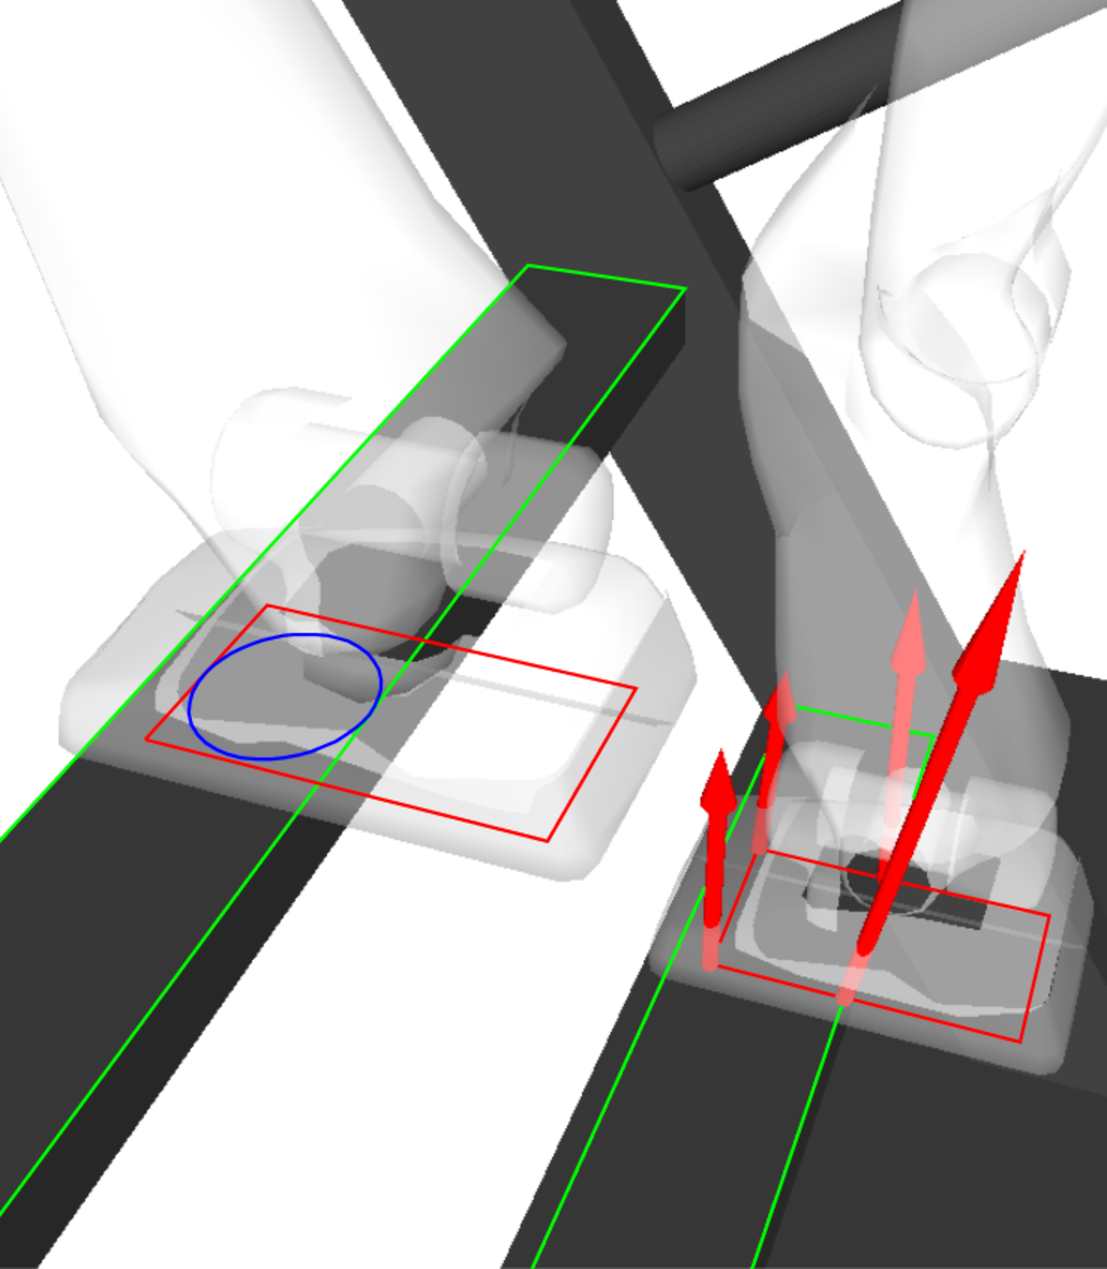
\includegraphics[width=0.95\linewidth]{hrp2_darpa_small_zoom_cut.pdf}}
%\label{fig:hrp2_darpa_zoom}
%\end{subfigure}
%\caption{HRP2 ladder climbing posture and up close view of the contact areas (green/red: contact polygons; blue: contact ellipse; red arrows: contact forces resultants)}
%\label{fig:hrp2_darpa_complete}
%\end{figure}

\begin{figure}[htpb]
  \centering
  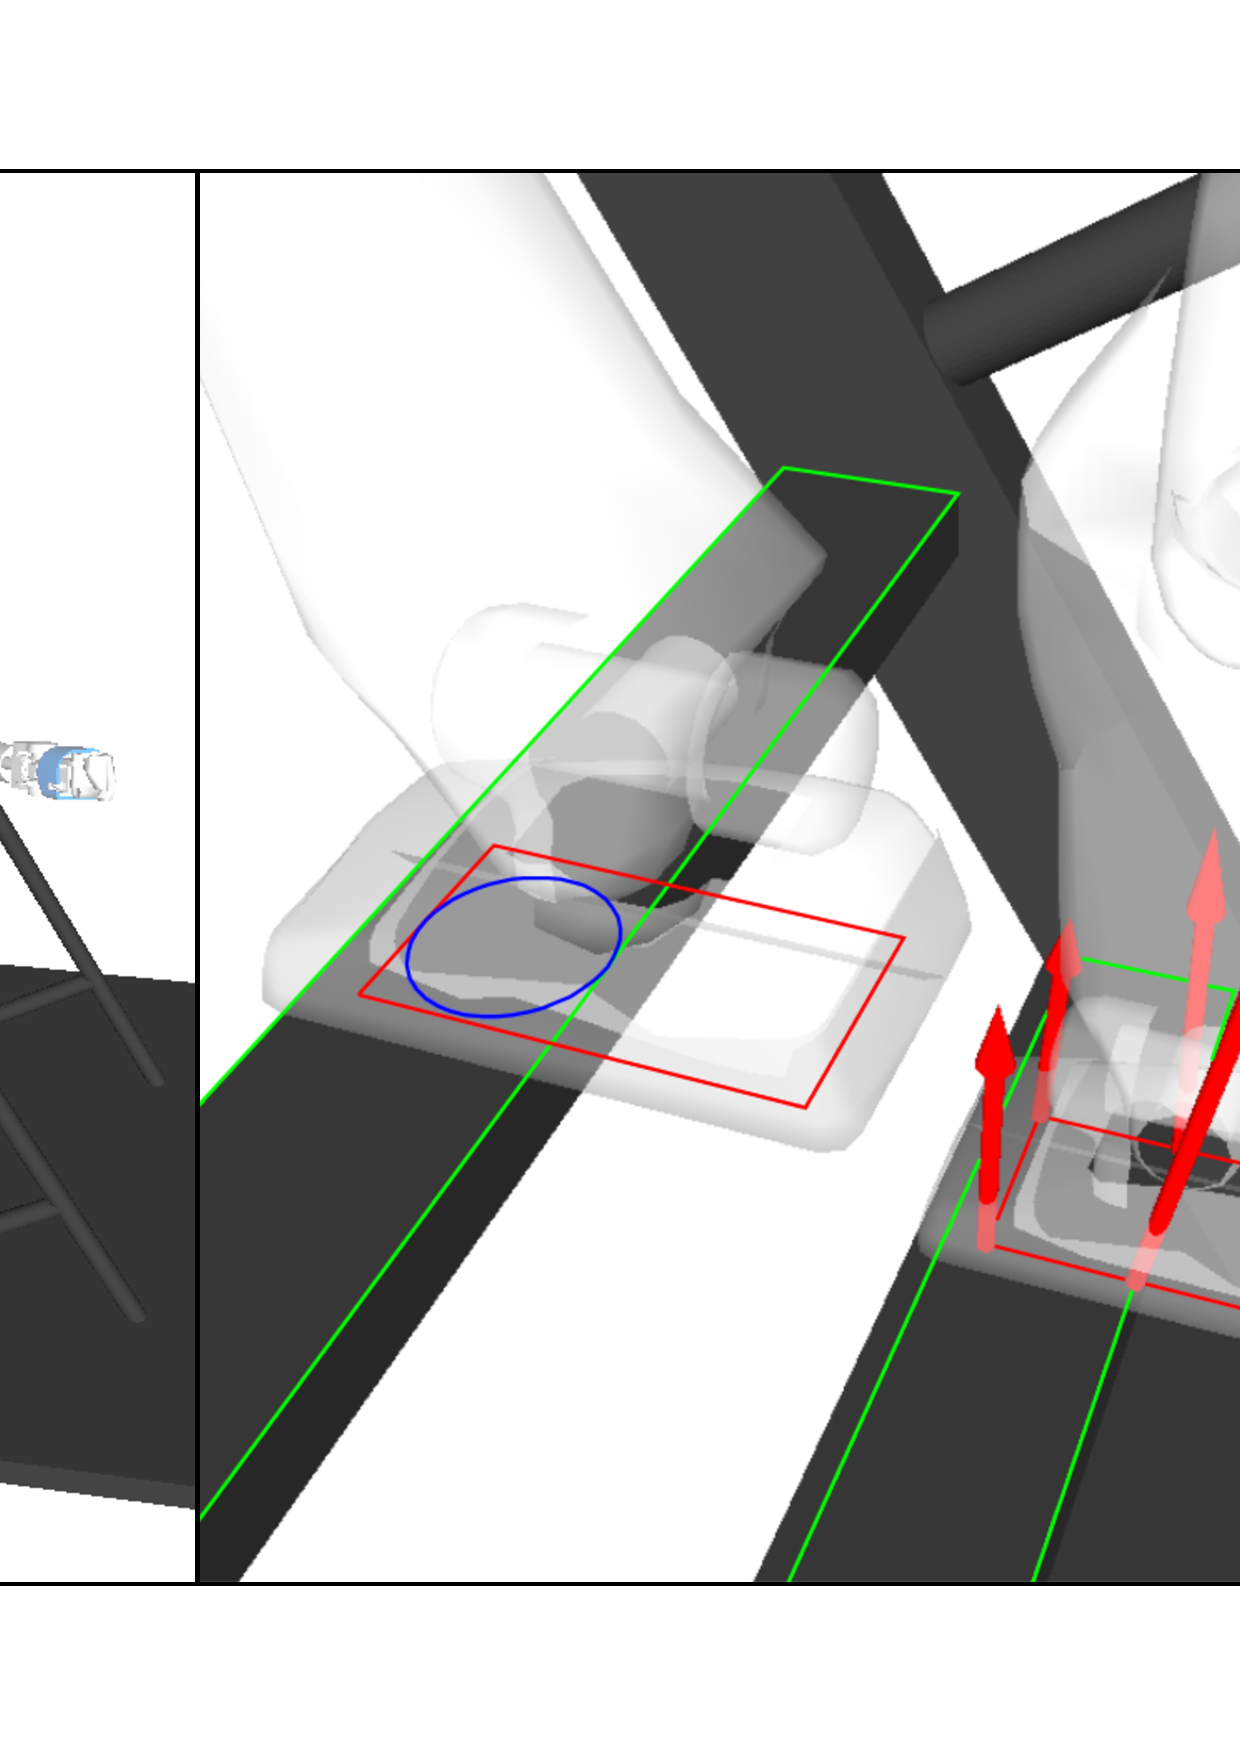
\includegraphics[width=0.8\linewidth]{hrp2_inclined_ladder.pdf}
  \caption{HRP2 ladder climbing posture and up close view of the contact areas (green/red: contact polygons; blue: contact ellipse; red arrows: contact forces resultants)}
\label{fig:hrp2_darpa_complete}
\end{figure}

\begin{figure*}
\centering
\setlength\fboxsep{0pt}
\setlength\fboxrule{1pt}
\fbox{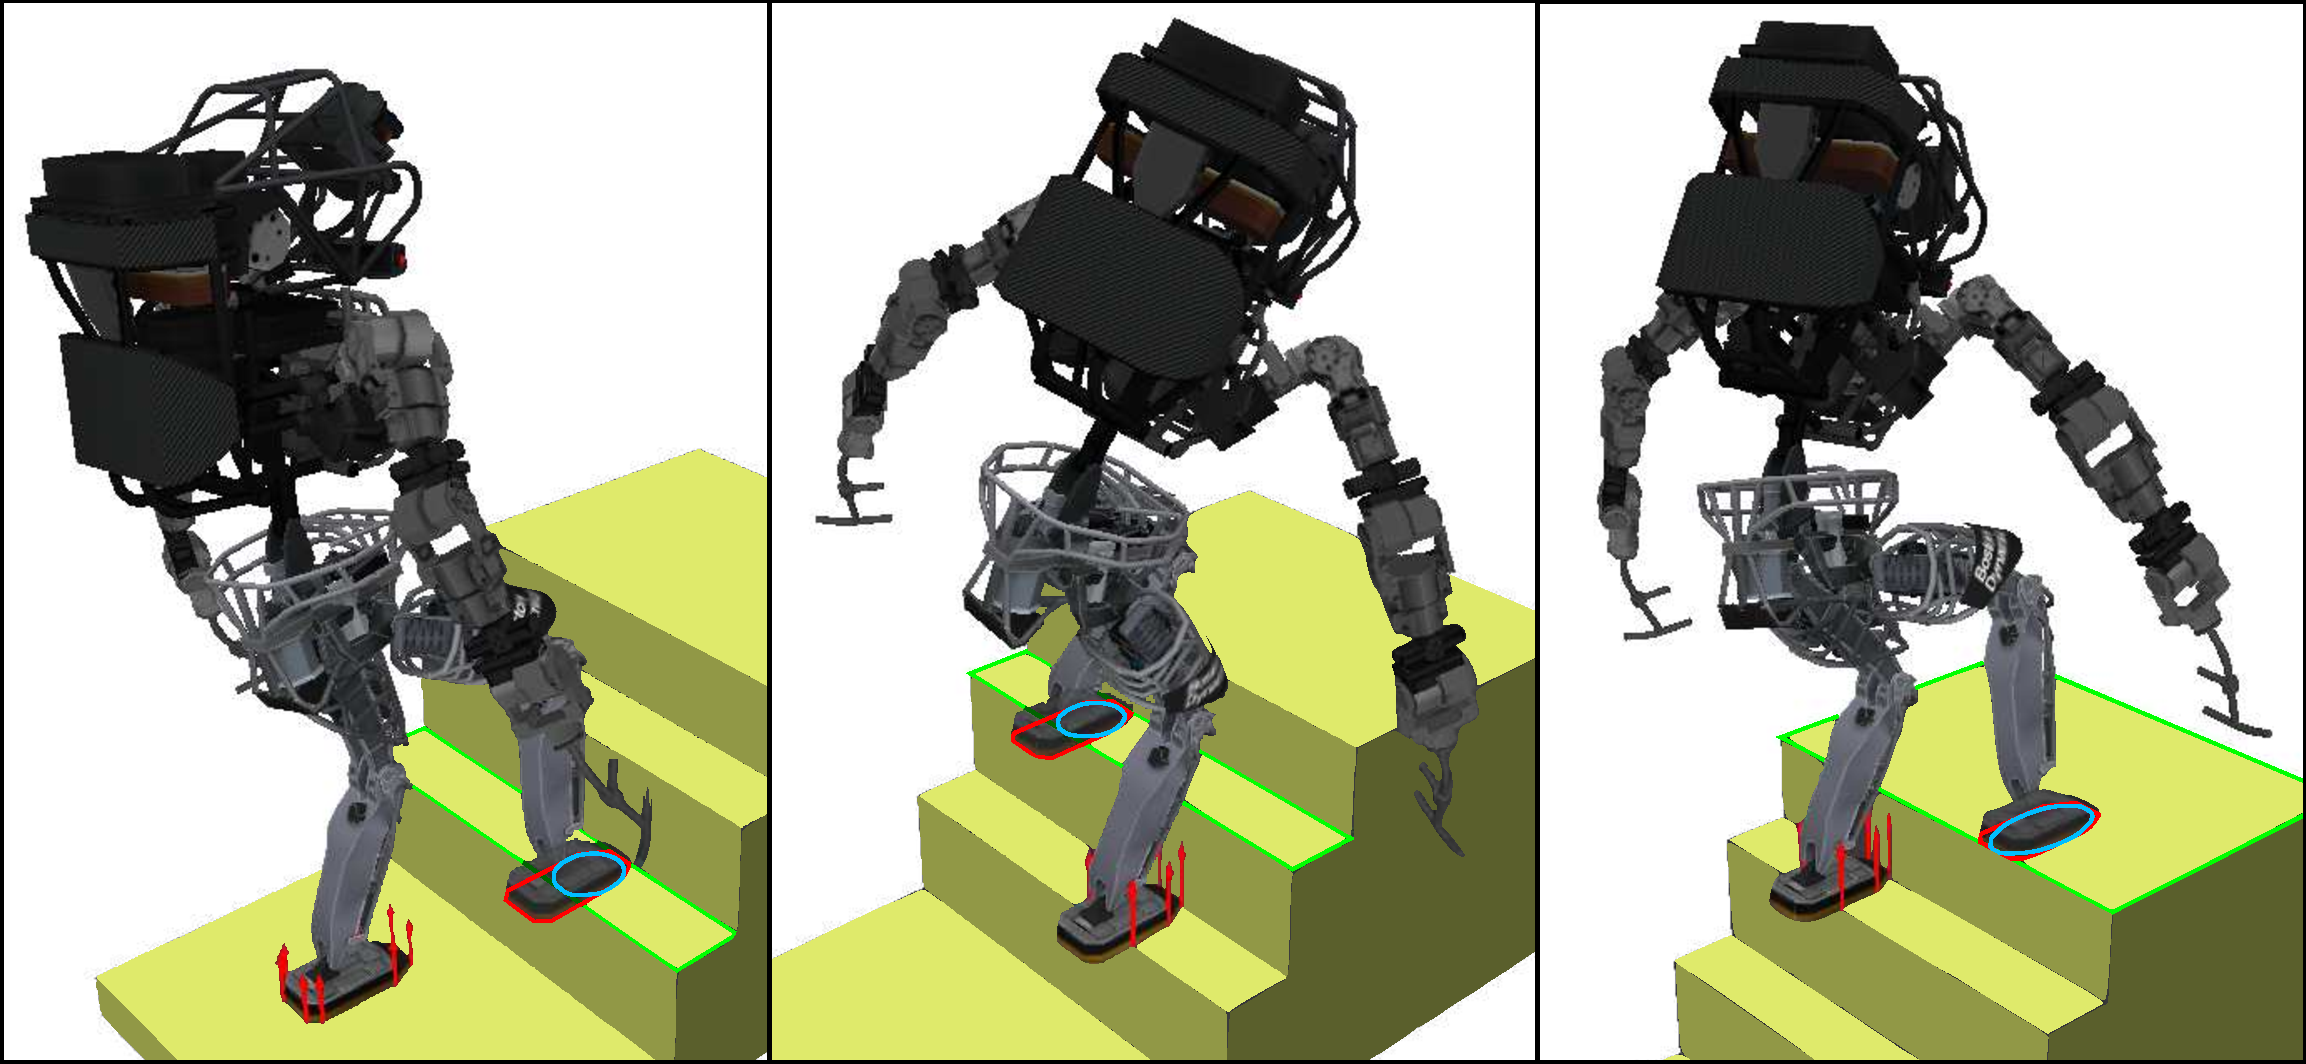
\includegraphics[width=0.95\linewidth]{fixed_atlas_1_2_3_yellow.pdf}}
\caption{Atlas climbing stairs with small steps by maximizing the size of the contact areas\\(green/red: contact polygons; blue: contact ellipse; red arrows: contact forces resultants)}
\label{fig:atlas_SmallStairs}
\end{figure*}



\subsubsection{Vertical ladder climbing}
\label{subsubsec:ladder}

%%%%%%%%%%%%%%%%%%%%%%%%%%%%%%%%%%%%%%%%%%%%%%%%%%%%%%%%%%%%%%%%%%%%%%%
%               SUBSUBSECTION VERTICAL LADDER CLIMBING                %
%%%%%%%%%%%%%%%%%%%%%%%%%%%%%%%%%%%%%%%%%%%%%%%%%%%%%%%%%%%%%%%%%%%%%%%

In the second example, we generate a posture in which the robot climbs a vertical ladder.
In this particular step, the robot is using its right foot and both hands to maintain its stability on top of the first rung of the ladder.
We search a posture that keeps those previous contacts and adds a geometrical contact between the left foot and the second rung of the ladder.
The result of that optimization can be observed on figure~\ref{fig:hrp2_jrl_complete}, with the robot posture on the left and a close-up look at the contact areas on the right.
The difficulty of this situation is that a contact has to be made with a very thin surface of the environment (the ladder rung).
%Usual contact generation method would reduce a lot the span of possible contact positions (by patching the robot's foot with a very small surface or by imposing a set of authorized contact positions).
%Whereas with our method, the contact configuration is found during the optimization process without requiring any extra human work.
The contact chosen by our software includes an ellipse which first axis is the width of the robot's foot and second axis is as thin as the ladder rung.
%One problem to expect is that numerical instability might happen if the surface of the rung is given too thin.
%But that would also happen with full inclusion constraints.
This example also illustrates one limitation of our method: it only considers planar contacts and if one wants to model a purely linear contact another contact model must be used, since our modeling of those singular cases is approximative.
%is the first step of the HRP-2 robot climbing a ladder.
%The two hands are in bilateral contact with the two side bars of the ladder, the left foot is fixed on the ground and is the only part of the robot involved in the stability.
%The right foot is to make a contact with the first rung of the ladder.
%The rungs of the ladder are modeled by rectangles with a 6mm width which approximates the contact line as explained in section~\ref{subsubsec:singular cases}.
%Therefore, the ellipse area maximization takes place in the intersection of the polygons representing the rung and the foot.
%The result of that optimization can be observed on ~\Figref{fig:ladder}{}.
%On the right of the simulation image is shown the disposition of the foot (in green) that is in geometrical non-inclusive contact with a rung (in blue) and the optimal ellipse that has been found.


%From a planning point of view, this particular result is obviously not achievable as the right leg of the robot goes through the ladder, this will be discussed in the next section.
%Yet, the posture is perfectly valid as it respects of the constraints of problem~(\Eqref{eq:PG_chap2}).
%This example illustrates our method in a multi-contact environment with almost linear contacts.
%



\subsubsection{Climbing Stairs}
\label{subsubsec:smallStairs}

%%%%%%%%%%%%%%%%%%%%%%%%%%%%%%%%%%%%%%%%%%%%%%%%%%%%%%%%%%%%%%%%%%%%%%%
%                   SUBSUBSECTION CLIMBING STAIRS                     %
%%%%%%%%%%%%%%%%%%%%%%%%%%%%%%%%%%%%%%%%%%%%%%%%%%%%%%%%%%%%%%%%%%%%%%%

In a third simulation, the ATLAS robot climbs a flight of stairs.
All the steps are too small for the robot to put its entire foot on.
Therefore, it has to make a non-inclusive contact and we propose to maximize the size of the contact area with the ellipse included in it, as explained in Section~\ref{subsubsec:optim-ellipse-area}.
The size of the contact area is limited by the fact that the foot cannot penetrate the wall behind each step.
On~\Figref{fig:atlas_SmallStairs}, we present 3 postures generated in this environment.
On each of those postures, we see that the ellipse's size is maximized until the foot enters in collision with the vertical wall behind each step.
And when possible, like on the last step, the contact area is maximized without collision limitation and the foot is positioned as fully included in the support surface.
We can see here that even when the size of the ellipse is maximized while competing with other nonlinear constraints like collision avoidance, our method still works well and leads us to a satisfactory solution.
It has been used to actually make the robot climb a vertical ladder and presented in~\cite{vaillant:autonomousrobots:2016} and~\cite{vaillant:humanoids:2014}.

%Under each simulation result, an image presents the disposition of the foot (in green) that is in geometrical non-inclusive contact with a step (in blue) and the optimal ellipse that has been found.
%It has to be noted that the green contact surface under a foot of the robot (green rectangle) is actually smaller than the actual foot due to our use of security margin for stability reason when experimenting with real robot and take into account an un-modeled flexibility at the ankle.
%That is why, with the collision avoidance activated between the foot and the next step, it seems that the foot is still far from the limit of the step (blue rectangle).
%Actually the foot is almost in collision with the vertical part of the next step.
%We decided not to present the initial and final steps of this hypothetical movement because they do not bear any interesting aspect as they both consist of the robot standing on a large flat surface.

%\begin{figure*}
%\centering
%\begin{subfigure}{.319\textwidth}
%  \centering
%  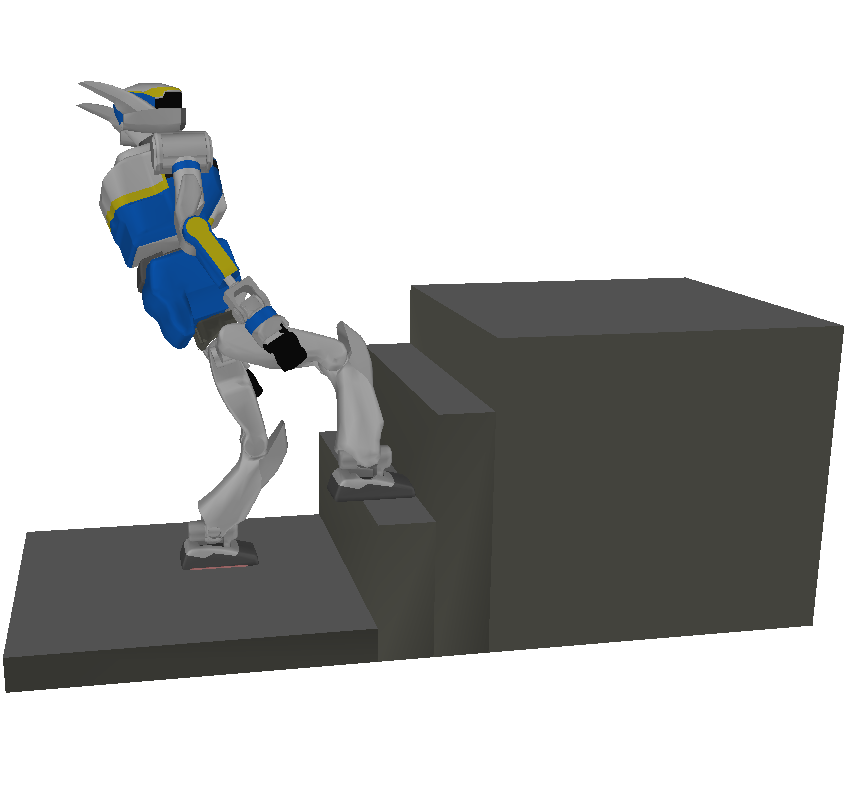
\includegraphics[width=\linewidth]{SmallStairs2.png}
%\end{subfigure}%
%\begin{subfigure}{.3\textwidth}
%  \centering
%  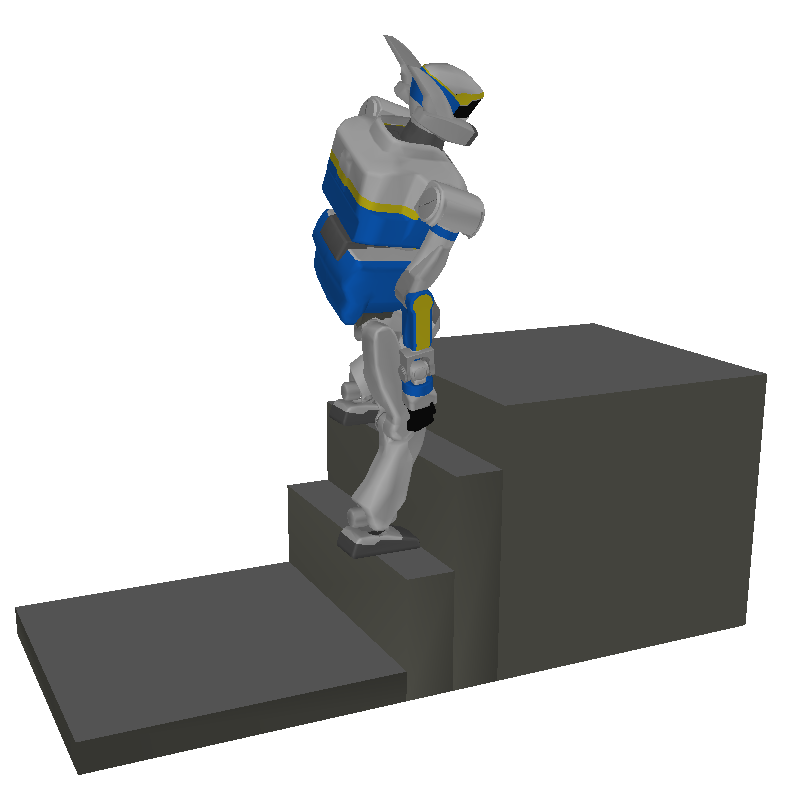
\includegraphics[width=\linewidth]{SmallStairs3.png}
%\end{subfigure}
%\begin{subfigure}{.3\textwidth}
%  \centering
%  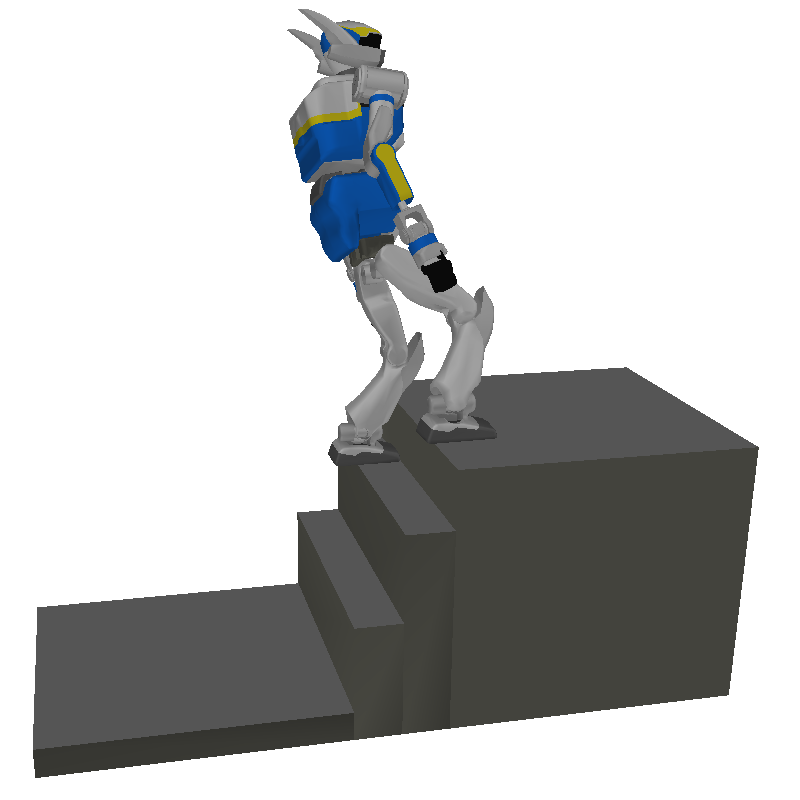
\includegraphics[width=\linewidth]{SmallStairs4.png}
%\end{subfigure}
%\caption{Using non-inclusive contacts for ladder climbing}
%\label{fig:hrp2_SmallStairs}
%\end{figure*}



\subsubsection{Walking along a path made of small objects}
\label{subsubsec:riviere}

%%%%%%%%%%%%%%%%%%%%%%%%%%%%%%%%%%%%%%%%%%%%%%%%%%%%%%%%%%%%%%%%%%%%%%%
%      SUBSUBSECTION WALKING ALONG A PATH MADE OF SMALL OBJECTS       %
%%%%%%%%%%%%%%%%%%%%%%%%%%%%%%%%%%%%%%%%%%%%%%%%%%%%%%%%%%%%%%%%%%%%%%%

In the last simulation, the HRP-2 robot has to cross a gap by making contacts
with small surfaces.
As for the previous simulation, the two objects
with which the feet of the robot will be in contact are too small for making a
complete contact, instead, non-inclusive geometric contacts are found by
maximizing the area of an ellipse that fits in the intersection of the polygons
involved in the contact.
Results are presented in figure~\ref{fig:riviere}.
As we can see, the feet turns slightly, to be more aligned with the support
surfaces, yet they do not become completely aligned with these supports, which would permit to get the biggest ellipse area.
This is due to the fact that a posture cost is competing with the area cost, yielding this compromise.
Under each simulation result, an image presents the disposition of the foot (in green) that is in geometrical non-inclusive contact with a step (in blue) and the optimal ellipse that has been found.
%We decided not to present the initial and final steps of this hypothetical movement because they do not bear any interesting aspect as they both consist of the robot standing on a large flat surface.

\begin{figure*}[!htb]
  \centering
  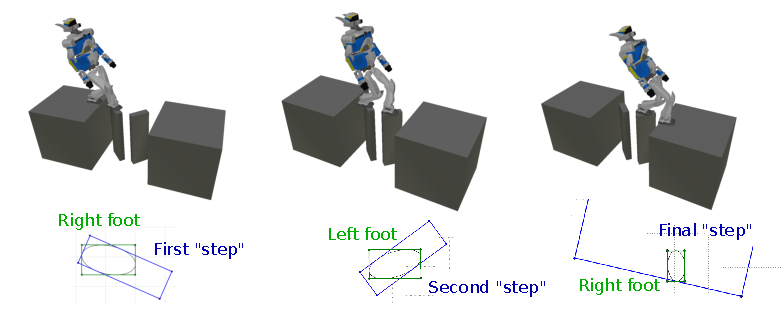
\includegraphics[width=0.95\textwidth]{riviere3steps.pdf}
  \caption{Simulation results for crossing a gap by walking on small items}
\label{fig:riviere}
\end{figure*}



\subsection{Discussion and conclusion}

%%%%%%%%%%%%%%%%%%%%%%%%%%%%%%%%%%%%%%%%%%%%%%%%%%%%%%%%%%%%%%%%%%%%%%%
%          SUBSECTION DISCUSSION AND CONCLUSION                       %
%%%%%%%%%%%%%%%%%%%%%%%%%%%%%%%%%%%%%%%%%%%%%%%%%%%%%%%%%%%%%%%%%%%%%%%

Generating arbitrarily shaped contact areas proved to be doable very simply in an optimization based posture generation module.
We focused on writing constraints that have continuous gradients since the posture generation problem is dominantly smooth.
Hence, our geometric contact model can be useful for other optimization based purposes, for example, control or trajectory optimization, and any gradient-based descent scheme which handles inequalities (e.g.~\cite{escande:icra:2010}).
While we were expecting an increase of computation time due to the addition of new variables in the problem (5 more for a total of 80--100 variables)
we noticed that the timings obtained with this method are sensibly the same that with our previous version of the posture generator with full contact surface inclusion.
Consequently, this method offering a richer contact search (exploration) during planning comes without degrading computation time.
In fact, it truly allows us to substantially reduce the time spent by the user in ad-hoc tuning the shapes of the contact patches, or fixing the contact positions that were previously done by hand.
Also, it is fairly easy to implement and extends multi-contact planning algorithms like the one described in~\cite{escande:ras:2013} to give it richer planning possibilities.
This method extends straightforwardly to point cloud data as far as polygonal convex patches can be extracted.
But one of its limitation is that in its current form, it cannot handle contacts with non-convex surfaces.

%There are several opportunities for future work.
%For example, we could improve the generality of our contact constraint formulation even further to manage linear and punctual contacts without the approximations we currently use.
%Also we could extend our method to allow dealing with non-convex surfaces.
%And finally we would like to apply our method to other fields that use contact generation, like trajectory or control optimization.
%While we were expecting an increase of computation time due to the addition of new variables in the problem (5 more for a total of 80-100 variables), we were surprised by the obtained timings, around $10s$ while a usual posture generation is less than $1s$.
%Part of this increase is obviously due to the fact that we used finite differences to compute the gradients of the new constraints and objectives, and one of the immediate on-going works is to derive and implement efficiently analytical gradients.
%Still, we will also investigate more thoroughly how the new constraints interact with the existing ones to look for potential other causes for this increase.

%Finally, on a planning point of view, ~\Figref{fig:ladder} shows us a new challenge: while the posture found is perfectly correct as the robot is stable, not colliding with its environment and the contacts are where we asked them to be, the posture is obviously difficult to attain, if possible at all.
%We will need to investigate what type of heuristic to use to avoid this kind of results in the middle of a plan.


\section{Torque derivation}
\label{sec:torque_derivation}

%%%%%%%%%%%%%%%%%%%%%%%%%%%%%%%%%%%%%%%%%%%%%%%%%%%%%%%%%%%%%%%%%%%%%%%
%                     SECTION TORQUE DERIVATION                       %
%%%%%%%%%%%%%%%%%%%%%%%%%%%%%%%%%%%%%%%%%%%%%%%%%%%%%%%%%%%%%%%%%%%%%%%

In this section, we present an efficient algorithm to compute the Jacobian matrix of the robot's joint torques with respect to all its articular variables and the variables involved in the expression of the external forces applied to this robot.
The evaluation of the joint torques Jacobian matrix is useful to solve optimization problems in which the torques are involved in the constraints or in the cost function.
The computation of the joint torques Jacobian matrix is done by differentiating algorithm~\ref{alg:IS}.
In most cases, the acceleration of gravity could be replaced by its value on earth $\mathbf{a_c} = \vec{0}$ and $\mathbf{a_f} = g \vec{z}$.
For the sake of generality, we keep it as $\mathbf{a_c}$ and $\mathbf{a_f}$ in the algorithm description, which could be useful if the robot is in a moving vehicle, for example.
We first write algorithm~\ref{alg:IS} in its matrix form (which is more convenient for its derivation).

\begin{algorithm}
  \caption{Inverse Static algorithm on Matrix Form}
\label{alg:ISmatrix}
\begin{algorithmic}
  \For{$i = 0:n_B$}\\
  $f^G_i =
  \begin{bmatrix}
    \mathbf{m}^{G}_i \\ \mathbf{f}^{G}_i
  \end{bmatrix}
  =
  \mathbf{I}^W
  \begin{bmatrix}
    {{}^i\mathbf{R}_W} & \mathbf{0} \\
    -{{}^i\mathbf{R}_W}\widehat{{}^i\mathbf{t}_W} & {{}^i\mathbf{R}_W} \\
  \end{bmatrix}
  \begin{bmatrix}
    \mathbf{a_c} \\ \mathbf{a_f}
  \end{bmatrix}
  -
  \begin{bmatrix}
    {{}^i\mathbf{R}_W} & -{{}^i\mathbf{R}_W}\widehat{{}^i\mathbf{t}_W} \\
    \mathbf{0} & {{}^i\mathbf{R}_W} \\
  \end{bmatrix}
  \begin{bmatrix}
    \mathbf{m}^{ext}_i \\ \mathbf{f}^{ext}_i
  \end{bmatrix}
  $
  \EndFor{}
  \For{$i = n_J-1:0$}
  \State$\tau_i = {f^G_i}^T S_i$
  \If{$pred(i) \neq -1$}
  \State$f^G_{pred(i)} \leftarrow
  \begin{bmatrix}
    \mathbf{m}^{G}_{pred(i)} \\ \mathbf{f}^{G}_{pred(i)}
  \end{bmatrix}
  +
  \begin{bmatrix}
    {\mathbf{R}^{PtS}_i}^T & \widehat{\mathbf{t}^{PtS}_i}{\mathbf{R}^{PtS}_i}^T \\
    \mathbf{0} & {\mathbf{R}^{PtS}_i}^T \\
  \end{bmatrix}
  \begin{bmatrix}
    \mathbf{m}^{G}_i \\ \mathbf{f}^{G}_i
  \end{bmatrix}
  $
  \EndIf{}
  \EndFor{}
\end{algorithmic}
\end{algorithm}

The variables of this algorithm w.r.t. which we need to differentiate it, are the configuration of the robot $q$ and the variables of the external wrenches which can themselves depend on $q$ and some other variables $y$, for example, in the case of a contact with another robot, the application point and value of those forces depend on $q$ and on the configuration of the other robot.
We denote $\dim(q)$ and $\dim(y)$ the dimensions of $q$ and $y$ respectively.
We assume that the derivatives of $m_i^{ext}$ and $f_i^{ext}$: $\frac{\partial m_i^{ext}}{\partial q}$, $\frac{\partial m_i^{ext}}{\partial y}$, $\frac{\partial f_i^{ext}}{\partial q}$, and $\frac{\partial f_i^{ext}}{\partial y}$ are known.

Besides $m_i^{ext}$ and $f_i^{ext}$, all the quantities of the algorithm depend only on $q$.
Therefore, the derivation w.r.t $y$ is trivial and is automatically computed by our final algorithm.
From here we will focus on the derivation w.r.t $q$.

Recall the expression of the Jacobian of a robot's body:
\begin{equation}
  \mathbf{Jac}^W_i =
  \begin{bmatrix}
    \frac{\partial {}^i\mathbf{R}_W}{\partial q_0} & \cdots &
    \frac{\partial {}^i\mathbf{R}_W}{\partial q_j} & \cdots &
    \frac{\partial {}^i\mathbf{R}_W}{\partial q_{dof}} \\
    \frac{\partial {}^i\mathbf{t}_W}{\partial q_0} & \cdots &
    \frac{\partial {}^i\mathbf{t}_W}{\partial q_j} & \cdots &
    \frac{\partial {}^i\mathbf{t}_W}{\partial q_{dof}}
  \end{bmatrix}
=
  \begin{bmatrix}
    \omega_{i,0} & \cdots &
    \omega_{i,j} & \cdots &
    \omega_{i,dof} \\
    v_{i,0} & \cdots &
    v_{i,j} & \cdots &
    v_{i,dof}
  \end{bmatrix}
\end{equation}

Note the following relations that make use of the robot's Jacobian to compute derivatives:
\begin{align}
  \frac{\partial {}^i\mathbf{R}_W \mathbf{u}}{\partial q_j}
  &= {}^i\mathbf{R}_W \mathbf{u} \wedge \omega_{i,j}
  = {}^i\mathbf{R}_W \widehat{\mathbf{u}} \omega_{i,j}
  \\
  \frac{\partial {}^i\mathbf{R}_W {}^i\mathbf{t}_W\wedge \mathbf{u}}{\partial q_j}
  &= {}^i\mathbf{R}_W \mathbf{v}_{i,j} \wedge \mathbf{u}
  + {}^i\mathbf{R}_W \left({}^i\mathbf{t}_W\wedge\mathbf{u}\right) \wedge \omega_{i,j}\\
  &= -{}^i\mathbf{R}_W \widehat{\mathbf{u}} \mathbf{v}_{i,j}
  + {}^i\mathbf{R}_W \widehat{\left(\widehat{{}^i\mathbf{t}_W}\mathbf{u}\right)} \omega_{i,j}
\end{align}

Let's differentiate the first equation of~\ref{alg:ISmatrix} w.r.t $q_j$.

\begin{align}
  A &=
  \begin{bmatrix}
    {{}^i\mathbf{R}_W} & \mathbf{0} \\
    -{{}^i\mathbf{R}_W}\widehat{{}^i\mathbf{t}_W} & {{}^i\mathbf{R}_W} \\
  \end{bmatrix}
  \begin{bmatrix}
    \mathbf{a_c} \\ \mathbf{a_f}
  \end{bmatrix} \\
  B &=
  \begin{bmatrix}
    {{}^i\mathbf{R}_W} & -{{}^i\mathbf{R}_W}\widehat{{}^i\mathbf{t}_W} \\
    \mathbf{0} & {{}^i\mathbf{R}_W} \\
  \end{bmatrix}
  \begin{bmatrix}
    \mathbf{m}^{ext}_i \\ \mathbf{f}^{ext}_i
  \end{bmatrix} \\
  f^G_i &= \mathbf{I}^W A-B\\
  \frac{\partial A}{\partial q_j} &=
  \begin{bmatrix}
    {}^i\mathbf{R}_W \widehat{\bf ac} \omega_{i,j}\\
    -{{}^i\mathbf{R}_W}\widehat{\left(\widehat{{}^i\mathbf{t}_W}{\bf ac} \right)}\omega_{i,j}
    + {{}^i\mathbf{R}_W}\widehat{\bf ac} v_{i,j} + {}^i\mathbf{R}_W \widehat{\bf af} \omega_{i,j}\\
  \end{bmatrix}
  \\
  \frac{\partial B}{\partial q_j} &=
  \begin{bmatrix}
    - {{}^i\mathbf{R}_W}\widehat{\left(\widehat{{}^i\mathbf{t}_W}\bf \mathbf{f}^{ext}_i \right)}\omega_{i,j}
    + {{}^i\mathbf{R}_W}\widehat{\bf \mathbf{f}^{ext}_i} v_{i,j} + {}^i\mathbf{R}_W \widehat{\bf \mathbf{m}^{ext}_i} \omega_{i,j}\\
    {}^i\mathbf{R}_W \widehat{\bf \mathbf{f}^{ext}_i} \omega_{i,j}\\
  \end{bmatrix}
  \\&+
  \begin{bmatrix}
    {{}^i\mathbf{R}_W} & -{{}^i\mathbf{R}_W}\widehat{{}^i\mathbf{t}_W} \\
    \mathbf{0} & {{}^i\mathbf{R}_W} \\
  \end{bmatrix}
  \begin{bmatrix}
    \frac{\partial \mathbf{m}^{ext}_i}{\partial q} \\ \frac{\partial \mathbf{f}^{ext}_i}{\partial q}
  \end{bmatrix}
\end{align}

We rearrange the equations in order to make the jacobian appear.
Putting all the pieces of $\omega$ and $v$ together allows grouping all the j-derivatives to obtain the derivative of $f^G_i$ with a single equation.

\begin{align}
  \bf M &=
  \begin{bmatrix}
    {}^i\mathbf{R}_W \widehat{\bf ac}  & 0\\
    -{{}^i\mathbf{R}_W}\widehat{\left(\widehat{{}^i\mathbf{t}_W}\bf ac \right)}
    + {}^i\mathbf{R}_W \widehat{\bf af}  & {{}^i\mathbf{R}_W}\widehat{\bf ac} \\
  \end{bmatrix}
  \\
  \bf N &=
  \begin{bmatrix}
    - {{}^i\mathbf{R}_W}\widehat{\left(\widehat{{}^i\mathbf{t}_W}\bf \mathbf{f}^{ext}_i \right)} + {}^i\mathbf{R}_W \widehat{\bf \mathbf{m}^{ext}_i} & {{}^i\mathbf{R}_W}\widehat{\bf \mathbf{f}^{ext}_i} \\
    {}^i\mathbf{R}_W \widehat{\bf \mathbf{f}^{ext}_i} & 0\\
  \end{bmatrix}
  \\
  \frac{\partial f^G_i}{\partial q} &= (\mathbf{I}^W \mathbf{M} - \mathbf{N})\mathbf{Jac}^W_i
  +
  \begin{bmatrix}
    {{}^i\mathbf{R}_W} & -{{}^i\mathbf{R}_W}\widehat{{}^i\mathbf{t}_W} \\
    \mathbf{0} & {{}^i\mathbf{R}_W} \\
  \end{bmatrix}
  \begin{bmatrix}
    \frac{\partial \mathbf{m}^{ext}_i}{\partial q} \\ \frac{\partial \mathbf{f}^{ext}_i}{\partial q}
  \end{bmatrix}
\end{align}

The derivation of the second equation is obvious:

\begin{align}
  \tau_i &= {f^G_i}^T S_i \\
  \frac{\partial \tau_i}{\partial q} &= S_i^T \frac{\partial f^G_i}{\partial q} \\
\end{align}

Note the following relations:
\begin{align}
  \frac{\partial {\mathbf{R}_i^J}^T \mathbf{u}}{\partial q_j}
  &= - S^R_{i,j} \wedge ({\mathbf{R}_i^J}^T \mathbf{u})
  = \widehat{({\mathbf{R}_i^J}^T \mathbf{u})} S^R_{i,j}
  \\
  \frac{\partial\mathbf{t}^J_i\wedge {\mathbf{R}_i^J}^T  \mathbf{u}}{\partial q_j}
  &= S^t_{i,j} \wedge \left({\mathbf{R}_i^J}^T \mathbf{u}\right)
  - \mathbf{t}^J_i \wedge \left( S^R_{i,j} \wedge \left({\mathbf{R}_i^J}^T \mathbf{u}\right)\right) \\
  &= -\widehat{({\mathbf{R}_i^J}^T \mathbf{u})} S^t_{i,j}
  + \left(\left({\mathbf{R}_i^J}^T \mathbf{u}\right) \cdot {\mathbf{t}^J_i}^T
  - \left( {({\mathbf{R}_i^J}^T \mathbf{u})}^T \cdot \mathbf{t}^J_i\right) \mathbf{I}_3\right)S_{i,j}^R\\
\end{align}

The last equation's derivation goes as follows:

\begin{align}
  f^G_{pred(i)} & \leftarrow f^G_{pred(i)} +
  \begin{bmatrix}
    {\mathbf{R}^{PtS}_i}^T & \widehat{\mathbf{t}^{PtS}_i}{\mathbf{R}^{PtS}_i}^T \\
    \mathbf{0} & {\mathbf{R}^{PtS}_i}^T \\
  \end{bmatrix}
  \begin{bmatrix}
    \mathbf{m}^{G}_i \\ \mathbf{f}^{G}_i
  \end{bmatrix}
  \\
  & =f^G_{pred(i)} + \begin{bmatrix}
    {\mathbf{R}^{x}_i}^T & \widehat{\mathbf{t}^{x}_i}{\mathbf{R}^{x}_i}^T \\
    \mathbf{0} & {\mathbf{R}^{x}_i}^T \\
  \end{bmatrix}
  \begin{bmatrix}
    {\mathbf{R}^{J}_i}^T & \widehat{\mathbf{t}^{J}_i}{\mathbf{R}^{J}_i}^T \\
    \mathbf{0} & {\mathbf{R}^{J}_i}^T \\
  \end{bmatrix}
  \begin{bmatrix}
    \mathbf{m}^{G}_i \\ \mathbf{f}^{G}_i
  \end{bmatrix}
  \\
\end{align}

We define $K_i$ as:
\begin{equation}
  K_i =
  \begin{bmatrix}
    \widehat{({\mathbf{R}_i^J}^T \mathbf{m}^{G}_i)}
    + \left({\mathbf{R}_i^J}^T \mathbf{f}^{G}_i\right) \cdot {\mathbf{t}^J_i}^T
    - \left( {({\mathbf{R}_i^J}^T \mathbf{f}^{G}_i)}^T \cdot \mathbf{t}^J_i\right) \mathbf{I}_3
    & -\widehat{({\mathbf{R}_i^J}^T \mathbf{f}^{G}_i)} \\
    \widehat{({\mathbf{R}_i^J}^T \mathbf{f}^{G}_i)} & 0
  \end{bmatrix}
\end{equation}

\begin{equation}
    \frac{\partial f^G_{pred(i)}}{\partial q} \leftarrow \frac{\partial f^G_{pred(i)}}{\partial q} -
  \begin{bmatrix}
    {\mathbf{R}^{x}_i}^T & \widehat{\mathbf{t}^{x}_i}{\mathbf{R}^{x}_i}^T \\
    \mathbf{0} & {\mathbf{R}^{x}_i}^T \\
  \end{bmatrix}
  K_i \mathbf{S_i}
\end{equation}

In the following algorithm, we use the following notation $x$ to combine the variables $q$ and $y$:
\begin{equation}
  x = \begin{bmatrix}
    q & y
  \end{bmatrix}
\end{equation}

\begin{equation}
  \frac{\partial f_{ext}}{\partial x} =
  \begin{bmatrix}
    \frac{\partial \mathbf{m}^{ext}_i}{\partial q} & \frac{\partial \mathbf{m}^{ext}_i}{\partial y}
    \\
    \frac{\partial \mathbf{f}^{ext}_i}{\partial q} & \frac{\partial \mathbf{f}^{ext}_i}{\partial y}
  \end{bmatrix}
\end{equation}


The entire algorithm for calculating the torque jacobian is presented in Algorithm~\ref{alg:TJC}.

\begin{algorithm}[H]
\caption{Torque Jacobian Calculation}
\label{alg:TJC}
\begin{algorithmic}
  \State{Compute the Jacobian of generalized forces}
  \For{$i = 0:n_B$}
  \State$f^G_i =
  \mathbf{I}^W
  \begin{bmatrix}
    {{}^i\mathbf{R}_W} & \mathbf{0} \\
    -{{}^i\mathbf{R}_W}\widehat{{}^i\mathbf{t}_W} & {{}^i\mathbf{R}_W} \\
  \end{bmatrix}
  \begin{bmatrix}
    \mathbf{a_c} \\ \mathbf{a_f}
  \end{bmatrix}
  -
  \begin{bmatrix}
    {{}^i\mathbf{R}_W} & -{{}^i\mathbf{R}_W}\widehat{{}^i\mathbf{t}_W} \\
    \mathbf{0} & {{}^i\mathbf{R}_W} \\
  \end{bmatrix}
  \begin{bmatrix}
    \mathbf{m}^{ext}_i \\ \mathbf{f}^{ext}_i
  \end{bmatrix}
  $
  \State$\bf M =
    \begin{bmatrix}
    {}^i\mathbf{R}_W \widehat{\bf ac}  & 0\\
    -{{}^i\mathbf{R}_W}\widehat{\left(\widehat{{}^i\mathbf{t}_W}\bf ac \right)}
    + {}^i\mathbf{R}_W \widehat{\bf af}  & {{}^i\mathbf{R}_W}\widehat{\bf ac} \\
    \end{bmatrix}
    $
  \State$\bf N =
  \begin{bmatrix}
    - {{}^i\mathbf{R}_W}\widehat{\left(\widehat{{}^i\mathbf{t}_W}\bf \mathbf{f}^{ext}_i \right)}
    + {}^i\mathbf{R}_W \widehat{\bf \mathbf{m}^{ext}_i}
    & {{}^i\mathbf{R}_W}\widehat{\bf \mathbf{f}^{ext}_i} \\
    {}^i\mathbf{R}_W \widehat{\bf \mathbf{f}^{ext}_i} & 0\\
  \end{bmatrix}
  $
  \State$
  \frac{\partial f^G_i}{\partial x} = (\mathbf{I}^W \mathbf{M} - \mathbf{N})\begin{bmatrix}
      \mathbf{Jac_i^W} & \mathbf{0}_{6\times \dim(y)}
        \end{bmatrix}
  +
  \begin{bmatrix}
    {{}^i\mathbf{R}_W} & -{{}^i\mathbf{R}_W}\widehat{{}^i\mathbf{t}_W} \\
    \mathbf{0} & {{}^i\mathbf{R}_W} \\
  \end{bmatrix}
  \frac{\partial f_{ext}}{\partial x}
  $
  \EndFor{}
  \State{Compute the Jacobian of torques}
  \For{$i = n_J-1:0$}
  \State$\frac{\partial \tau_i}{\partial x} =
  \begin{bmatrix}
    \mathbf{S_i} & \mathbf{0}_{6\times \dim(y)}
  \end{bmatrix}^T \frac{\partial f^G_i}{\partial x}$
  \If{$pred(i) \neq -1$}
  \State$\mathbf{K} =
  \begin{bmatrix}
    \widehat{({\mathbf{R}_i^J}^T \mathbf{m}^{G}_i)}
    + \left({\mathbf{R}_i^J}^T \mathbf{f}^{G}_i\right) \cdot {\mathbf{t}^J_i}^T
    - \left( {({\mathbf{R}_i^J}^T \mathbf{f}^{G}_i)}^T \cdot \mathbf{t}^J_i\right) \mathbf{I}_3
    & -\widehat{({\mathbf{R}_i^J}^T \mathbf{f}^{G}_i)} \\
    \widehat{({\mathbf{R}_i^J}^T \mathbf{f}^{G}_i)} & 0
  \end{bmatrix}$
  \State$f^G_{pred(i)} \leftarrow f^G_{pred(i)} + {\mathbf{X}^{PtS}_i(q)}^{-*} f^G_i$
  \State$\frac{\partial f^G_{pred(i)}}{\partial x} \leftarrow \frac{\partial f^G_{pred(i)}}{\partial x} -
  \begin{bmatrix}
    {\mathbf{R}^{x}_i}^T & \widehat{\mathbf{t}^{x}_i}{\mathbf{R}^{x}_i}^T \\
    \mathbf{0} & {\mathbf{R}^{x}_i}^T \\
  \end{bmatrix}
  \mathbf{K} \cdot \begin{bmatrix}
    \mathbf{S_i} & \mathbf{0}_{6\times \dim(y)}
  \end{bmatrix}$
  \EndIf{}
  \EndFor{}
\end{algorithmic}
\end{algorithm}

This algorithm efficiently computes the exact joint torques Jacobian for a robotic system subject to any type of external forces.

\newpage
\section{On the use of lifted variables for Robotics Posture Generation}
\label{sec:liftedVariables}

%%%%%%%%%%%%%%%%%%%%%%%%%%%%%%%%%%%%%%%%%%%%%%%%%%%%%%%%%%%%%%%%%%%%%%%%%%%
% SECTION ON THE USE OF LIFTED VARIABLES FOR ROBOTICS POSTURE GENERATION  %
%%%%%%%%%%%%%%%%%%%%%%%%%%%%%%%%%%%%%%%%%%%%%%%%%%%%%%%%%%%%%%%%%%%%%%%%%%%

The goal of this thesis is, on the one hand, to enable writing more complex and various problems in simpler ways by improving the formulation of posture generation problems, and on the other hand, to improve and adapt the resolution methods for those problems.
This section focuses on the latter issue.
We formulate posture generation problems in an optimization friendly way in order to solve them using nonlinear constrained optimization algorithms.
In this section, we investigated the usage of the lifted optimization method presented in~\cite{Albersmeyer:2010:LNM:1958447.1958472} to the posture generation problems. In fact, the authors concluded that their method would be suitable for inverse kinematic problems.

The idea of lifting optimization is to consider a complex equation $F(q) = 0$ and decompose it into simpler functions $\{f_1, f_2, \ldots, f_m\}$ that all depend only on the original variable $q$ and on the output of functions of lower index eq.~(\ref{eq:simplerFunctions}) that are replaced by additional variables $\{w_1, w_2, \ldots, w_m\}$, that are called the `lifted variables'.

\begin{equation}
\label{eq:simplerFunctions}
  w_i = f_i(q, w_1, w_2, \ldots,w_{i-1}),\ \forall i\in[1,\ldots, m]
\end{equation}

Such that they can be used in a chain to recompose $F$:

\begin{align}
  F(q) &= f_F\left(q, w_1, w_2, \ldots, w_m\right)\\
       &= f_F\left(q, f_1(q), f_2(q,w_1), f_3(q,w_1,w_2), \ldots, f_m(q, w_1, \ldots, w_m-1)\right) \\
       &= f_F\left(q, f_1(q), f_2(q,f_1(q)), f_3(q,f_1(q),f_2(q,f_1(q))), \ldots, f_m(q, \ldots, f_{m-1}(q,\cdots))\right)
\end{align}

With this formulation and the additional lifted variables $w_i,\ i\in[1,\ldots, m]$, the problem $F(q) = 0$ can be rewritten as the following lifted problem:

\begin{equation}
\label{eq:lifted_variables}
  G(q,w) =
  \begin{pmatrix}
  f_1(q) - w_1 \\
  f_2(q,w_1) - w_2 \\
  f_3(q,w_1,w_2) - w_3 \\
  \vdots \\
  f_m(q,w_1,\ldots, w_{m-1}) - w_m \\
  f_F(q,w_1,\ldots, w_{m-1}, w_m)
  \end{pmatrix}
  =0
\end{equation}

This modified formulation can be used for any function of our optimization problem to reduce the complexity of individual equations at the cost of adding extra variables and constraints.
By reducing the complexity of the functions, which often results in reducing their polynomial degree, we ought to improve the quality of their quadratic approximations, which should lead to better convergence properties of the Newton scheme.

%The reason for expecting this approach to yield good results is that during the optimization process, at each step, a quadratic approximation of the function $F$ is used to compute the next iterate.
%If $F$ is a complicated function, the quadratic approximation may be quite far from $F$ and simpler functions may have better quadratic approximations, which should lead to better convergence properties of the Newton scheme.

One obvious drawback of this approach for solving nonlinear problems is the increased size of the linearized problem to solve at each iteration of the optimization.
Fortunately,~\cite{Albersmeyer:2010:LNM:1958447.1958472} propose an algorithmic trick leveraging the triangularity of the Jacobian of $G(q,w)$ to condense the lifted problem into a problem of the same size as the original one.
Thus, the resolution of each iteration should take approximately the same time as with the original problem.

The lifted variable approach is known to be superior to the non-lifted one in the problem of shooting methods for boundary value problems~\cite{osborne:1969:shooting}.
With good intuition, the authors of~\cite{Albersmeyer:2010:LNM:1958447.1958472} state that the lifting idea could be directly transferred in the context of kinematic chains found in robotics.
Indeed, as we state in Section~\ref{sec:forward_kinematics}, the equation that governs the transformation of a robot's end effector on body $i$, ${}^i X_W(q)$ is constructed iteratively and seems to be a good candidate for lifting.
If we consider a single chain robot with $m$ bodies, such that $\kappa (m) = \{0, 1, 2, \ldots m\}$ the ${}^m X_W(q) = X_\text{goal}$ can straightforwardly be lifted as follows:

\begin{equation}
\label{eq:robot_lift}
  G(q,w) =
  \begin{pmatrix}
  {}^1 X_W(q) - w_1 \\
  {}^2 X_1(q)\cdot w_1 - w_2\\
  {}^3 X_2(q)\cdot w_2 - w_3 \\
  \vdots \\
  {}^m X_{m-1}(q)\cdot w_{m-1} - w_{m-1} \\
  w_{m-1} - X_\text{goal}
  \end{pmatrix}
  =0
\end{equation}

The transformation of a body is used in almost all the constraints and cost functions of posture generation problems, thus, we can use this lifting approach in most functions of our problems.
This formulation can be generalized to more complex robots by considering/lifting only the bodies in the direct chain from the base to the end effector.

\subsection{Lifting Algorithm}
\label{subsec:LiftingAlgorithm}

In order to explore the capabilities of optimization on lifted problems, we developed and studied several lifting approaches based on different lifting criterion.
A lifting criterion is a criterion that should be satisfied as best as possible by all the functions present at the end of the lifting process.
For example, the degree of a polynomial can be a used, one could require that all the functions are polynomials of at most degree $m$.
In~\ref{eq:robot_lift}, we lifted based one the criterion that each function should only contain a single joint transformation.

Let us consider an example with a simple planar 2 axis robot, with 2 successive links of length 1 attached by revolute joints.
Its articular variables are denoted $q = (q_1, q_2)$ and the expression of the end-effector's (EE) position is the following:
\begin{equation}
  \left(\begin{array}{c}
    \cos\!\left(q_{1}\right) + \cos\!\left(q_{1}\right)\, \cos\!\left(q_{2}\right) - \sin\!\left(q_{1}\right)\, \sin\!\left(q_{2}\right)\\
    \sin\!\left(q_{1}\right) + \cos\!\left(q_{1}\right)\, \sin\!\left(q_{2}\right) + \cos\!\left(q_{2}\right)\, \sin\!\left(q_{1}\right)
  \end{array}\right)
  =
  \left(\begin{array}{c}
    \text{EE}_{x}(q)\\
    \text{EE}_{y}(q)
  \end{array}\right)
\label{eq:direct_position}
\end{equation}

Those equations are polynomials in the variables $\cos(q_1)$, $\sin(q_1)$, $\cos(q_2)$, $\sin(q_2)$.
Furthermore, they are polynomials of degree $1$ in each of those variables separately.
This observation extends to the case of any robot composed of the joints presented in Section~\ref{sec:joints_formulations} and that does not contain kinematic loops (kinematic loops are not considered in this thesis).
The operators `addition', `subtraction', `multiplication', `sinus' and `cosinus' are enough to describe the kinematics of a robot.

We developed a generic algorithm which allows to automatically lift symbolic functions, and in particular, polynomials of trigonometric functions, based on a given criterion.
To do so, we use symbolic variables. A symbolic equation can be seen as a graph of atomic operations (addition, multiplication, and other functions), which can, in turn, be explored and truncated at appropriate places where we insert additional variables.
Figure~\ref{fig:graph_direct} presents the graph of atomic operations for equation~\Eqref{eq:direct_position}, where the green circles represent the original variables, the yellow ones represent the lifted variables, the pink ones represent the atomic operations and the red circles represent the final atomic operations that lead to the end effector equations.
\begin{figure}
  \centering
  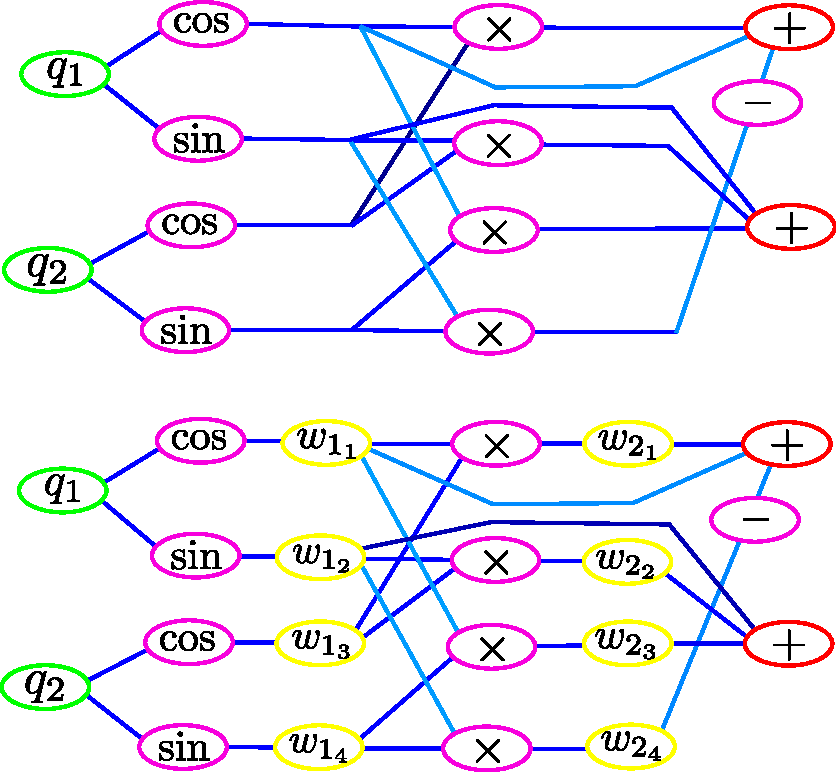
\includegraphics[width=0.65\textwidth]{graphDirectLiftedEEPos.pdf}
  \caption{Computation graph for end effector position of a 2 axis planar robotic arm. Top: Direct equations. Bottom: Lifted equations. Green circles represent the original variables, yellow the lifted ones, pink represent intermediary operations and red represent the final operation for the end effector equations}
\label{fig:graph_direct}
\end{figure}

To lift a set of equations, we explore the graph from left to right. At each node of the graph, we consider the sub-graph that lies on its left.
If this sub-graph violates our criterion, a lifting variable is added and replaces the sub-graph.
Then we iterate this process on the remaining graph until it does not violate the criterion.
Given that the equations to solve are polynomials in terms of the trigonometric functions, we decided to lift them based on a criterion of maximum degree of the lifted polynomials.
We define the degree function as the degree of a polynomial with the specificity that trigonometric functions are considered to be polynomials of infinite degree (and thus are always lifted, no matter the maximum degree criterion).
We also consider the option of eliminating or not the trigonometric functions.
By eliminating the trigonometric functions, we mean that we reformulate the problem so that, given a variable $x$ that appears in our equations in the forms $\cos(x)$ and/or $\sin(x)$, we introduce 2 new variables $s_x$ and $c_x$; replace all the occurrences of $\cos(x)$ by $c_x$ and all the occurrences of $\sin(x)$ by $s_x$, and to ensure the equivalence of the two formulations, we add the equation ${c_x}^2 + {s_x}^2=1$ to our problem.

For example, lifting the set of equation~\Eqref{eq:direct_position} with a maximum degree of 2 and without eliminating the trigonometric functions gives the following system, with all the $w_{i_j}$ being the additional lifted variables:
\begin{equation}
  \begin{array}{c}
  \textbf{Lifted Equations}\\
  \left(
    \begin{array}{c}
      \cos(q_1) = w_{1_1}\\
      \sin(q_1) = w_{1_2}\\
      \cos(q_2) = w_{1_3}\\
      \sin(q_2) = w_{1_4}\\
      w_{1_1}.w_{1_3} = w_{2_1}\\
      w_{1_2}.w_{1_3} = w_{2_2}\\
      w_{1_1}.w_{1_4} = w_{2_3}\\
      w_{1_2}.w_{1_4} = w_{2_4}
    \end{array}
  \right)\\
  \textbf{End-effector's position}\\
  \left(\begin{array}{c}
      w_{1_1} + w_{2_1} - w_{2_4} = EE_x\\
      w_{1_2} + w_{2_2} + w_{2_3} = EE_y
    \end{array}
  \right)\\
  \end{array}
\end{equation}
\label{eq:lifted_equations}

Adding to it the elimination of trigonometric functions gives the following system.
Note that here, all the equations are polynomials of degree at most 2, no trigonometric function is present, and the optimization variables are $\left(c_{q_1}, c_{q_2}, s_{q_1}, s_{q_2}\right)$ instead of $\left(q_1, q_2\right)$.

\begin{equation}
\begin{array}{c}
  \textbf{Lifted Equations}\\
  \left(\begin{array}{cc}
    c_{q_1}.c_{q_2} = w_{2_1}\\
    s_{q_1}.c_{q_2} = w_{2_2}\\
    c_{q_1}.s_{q_2} = w_{2_3}\\
    s_{q_1}.s_{q_2} = w_{2_4}\\
  \end{array}\right)\\
  \textbf{Additional equations}\\
  \left(\begin{array}{c}
    {c_{q_1}}^2 + {s_{q_1}}^2 = 1\\
    {c_{q_2}}^2 + {s_{q_2}}^2 = 1
  \end{array}\right)\\
  \textbf{End-effector's position}\\
  \left(\begin{array}{c}
    c_{q_1} + w_{2_1} - w_{2_4} = EE_x\\
    s_{q_1} + w_{2_2} + w_{2_3} = EE_y
  \end{array}\right)\\
  \textbf{Eliminated equations (Not used in further calculations)}\\
  \left(\begin{array}{c}
    \cos(q_1)  =  c_{q_1} \\
    \sin(q_1)  =  s_{q_1} \\
    \cos(q_2)  =  c_{q_2} \\
    \sin(q_2)  =  s_{q_2}
  \end{array}\right)\\
\end{array}
\label{eq:lifted_equations_trigo}
\end{equation}

This lifting methodology can be extended to most robotic systems.
We also developed a lifting method that follows the principle described in~\Eqref{eq:robot_lift}, in which case, we get another set of equations similar to~\Eqref{eq:lifted_equations}.

\subsection{Optimization on lifted variables}
\label{subsec:optimization_on_lifted_variables}

We want to estimate the gain in terms of performance that result from using a lifted formulation on a posture generation problem.
In order to do so, we implemented and/or used several optimization algorithms.

Given the lifted equations and their derivatives, it is straightforward to solve and compare the results obtained by the different solvers provided in Matlab (trust-region-reflective; interior-point; active-set and SQP) for the set of equations with or without lifting.
A limitation of our approach is that it does not allow us to easily use the condensed method presented in~\cite{Albersmeyer:2010:LNM:1958447.1958472} in the resolution of the problems because it is necessary to de-condensate and then update the problem between 2 iterations of the optimization.
The lifted condensed problem is meant to be equivalent to the lifted full-space problem (lifted non-condensed problem), in the sense that they generate the same optimization steps.
Solving lifted problems with or without using the condensation trick gives the same result in the same number of iterations.
The only difference is that with the lifted full-space problem, each iteration takes more time to compute.
In our study, this is not a problem, we want to evaluate the performances in terms of the number of iterations first, and if it appears that the lifted problem resolution outperforms the non-lifted, then we will implement the condensation trick for our problems and solvers, which will bring the per iteration time to be approximately the same as in the direct problem case.
Therefore, we only tried those algorithms on the direct problems (non-lifted problem) and the lifted full-space problems.

In addition to the Matlab solvers, we implemented the optimization algorithms proposed in~\cite{Albersmeyer:2010:LNM:1958447.1958472}, namely: the Lifted Newton, the Lifted Gauss-Newton and the Lifted SQP.
With the only difference that we use the symbolic expressions of all our function and compute the symbolic expressions of the Jacobians and Hessians of our problems, instead of using auto-differentiation methods.

We implemented the Newton and Gauss-Newton methods for condensed lifted problems and obtained the same results as the ones presented in paragraph 5.2 of~\cite{Albersmeyer:2010:LNM:1958447.1958472} that show the efficiency of a lifted approach in a specific kind of root finding problems.
Our problems require the use of nonlinear cost and constraints, thus, a Newton method is not sufficient to solve them, whereas an SPQ method is.

We implemented the lifted and direct SQP approaches as described in paragraph 3.2.3 of~\cite{Albersmeyer:2010:LNM:1958447.1958472}.
The hessian matrices in our problems are usually not symmetric positive definite, so we need to use a globalization method as well as a regularization of the Hessian to enforce convergence.
For globalization, we implemented some line search methods with Armijo and Wolfe conditions, as well as a filter with line search (see~\ref{ssub:the_filter_method}).
And for regularization, we approximate the full-space hessian matrix through BFGS updates (with Powell's correction) or SR1 updates.
We implemented different ways to initialize the lifted variables.
They can either be all initialized with zero value, or all random, or their initial value can be computed such that all the lifter equations are satisfied ($m$ first lines of~\ref{eq:lifted_variables}).
Those methods are presented in~\cite{bonnans:springer:2002}.
%All those methods are applied on the full-space iteration, during the update process of the optimization, the lifted and final equations are treated the same way.

%\subsection{Condensed BFGS update}
%\label{subsec:condensed_bfgs_update}
%In appendix, we propose a formulation of the condensed version of the BFGS algorithm.

%TODO Because it has not been used much and we didn't get any good results out of it, I'm not sure if I should present it or not\ldots

\subsection{Results, experimentation}
\label{subsec:Results}

In order to evaluate the performances of the lifting approach in the resolution of posture generation problems, we conducted many experiments in which we solved simple inverse kinematics problems with the different solvers and lifting methods available.

A difficulty that arises in that endeavor lays in the inherent combinatorial aspect on the choice of formulation and resolution method.
Indeed, we need to choose one item amongst each or the categories cited below:
\begin{itemize}
  \item Type of lifting method
  \begin{itemize}
    \item None, direct problem
    \item Lifted with maximum degree of 2
    \item Lifted based on Joints (one joint transformation per equation)
  \end{itemize}
  \item Treatment of trigonometric equations
  \begin{itemize}
    \item Keep trigonometric equations
    \item Eliminate trigonometric equations
  \end{itemize}
  \item Type of Solver
  \begin{itemize}
    \item Our custom SQP
    \item Matlab optimization toolbox {\tt fmincon} (active-set, interior point, SQP)
  \end{itemize}
  \item Type of initialization of the lifted variables
  \begin{itemize}
    \item Zeros
    \item Random
    \item Satisfying the lifted equations
  \end{itemize}
  \item Type of Hessian update
  \begin{itemize}
    \item None
    \item BFGS
    \item SR1
  \end{itemize}
  \item Type of globalization
  \begin{itemize}
    \item Wolfe
    \item Armijo
    \item Filter
  \end{itemize}
  \item Cost function
  \begin{itemize}
    \item None
    \item Norm 2 of articular parameters
  \end{itemize}
\end{itemize}
The number of possible combination of choices is large and grows with any new possibility added.

We devised a set of simple robots to be the toy examples of our experimentation.
We used fixed base robots with revolute joints only.
To study the influence of the number of degrees of freedom of a robot on the optimization performance, we studied planar robots composed of $n$ successive links of length 1 attached to one another by revolute joints.
We also studied a 7 axis 3D manipulator arm robot and a planar upper body robot with 2 arms.
Illustration of those different types of robots are given in figure~\ref{fig:robots}, where blue lines represent the links, red circles represent the revolute joints, green squares represent the origin of links, the biggest green square being the origin of the base link of the robot, and the red cross is the end effector.
\begin{figure}
  \centering
  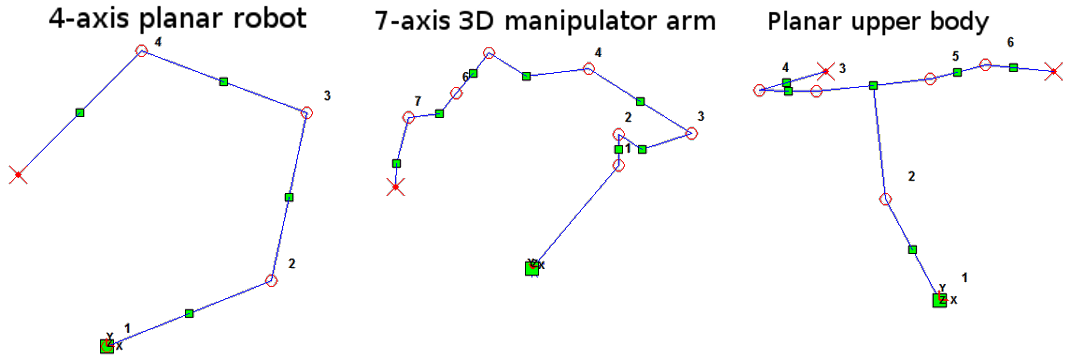
\includegraphics[width=0.98\textwidth]{robots.png}
  \caption{Examples of robots used}
\label{fig:robots}
\end{figure}

We propose to use the following test to compare the performances of different lifting methods for all our experiments:
\begin{enumerate}
  \item Choose a robot and a resolution method
  \item Generate 1000 pairs of initial configuration and end effector goal
  \item Solve the problem of finding a configuration in which the end effector reaches the goal for all the available formulations:
  \begin{itemize}
    \item Direct: Direct formulation
    \item Direct Trigo: Direct with trigonometric elimination
    \item Lifted: Lifted with maximum degree 2
    \item Lifted Trigo: Lifted with maximum degree 2 and trigonometric elimination
    \item Lifted Joint: Lifted based on joints
    \item Lifted Joint Trigo: Lifted based on joints and trigonometric elimination
  \end{itemize}
\end{enumerate}

This approach allows to fairly compare the performances of all lifting approaches on a given problem.
And to observe the influence of the number of degrees of freedom of the robot on those performances, we use the n-axis planar robot model.
We plot the average number of iterations needed to reach convergence against the number of degrees of freedom of the planar robot.
In figure~\ref{fig:lift_results} we present the results obtained for the resolution with our custom SQP, using BFGS updates and a filter line-search, without cost function, initializing all the variables randomly.
In figure~\ref{fig:lift_results2} we present the best case in favor of the lifted approach that we encountered, those results are obtained for the resolution with our custom SQP, using SR1 updates and a filter line-search, without cost function, initializing all the variables such that the lifted equations are satisfied.

\begin{figure}
\centering
\begin{tikzpicture}
\begin{axis}[
    %title={Custom SQP, BFGS updates, filter line-search, no cost function, random initialization},
    xlabel={DOF},
    ylabel={Iterations},
    xmin=2, xmax=12,
    ymin=5, ymax=20,
    xtick={0,2,4,6,8,10,12},
    ytick={0,5,10,15,20},
    legend pos=outer north east,
    ymajorgrids=true,
    grid style=dashed,
]
\addplot[color=blue,mark=x]
    coordinates {(2,8.628)(3,8.52)(4,9.271)(5,8.958)(6,7.928)(7,6.741)(8,7.908)(9,8.84)(10,8.145)(11,7.994)(12,6.634)};
\addplot[color=orange,mark=+]
    coordinates {(2,12.05)(3,11.83)(4,10.91)(5,10.26)(6,9.063)(7,8.39)(8,9.381)(9,10.03)(10,8.94)(11,8.717)(12,8.271)};
\addplot[color=yellow,mark=o]
    coordinates {(2,9.981)(3,10.69)(4,10.06)(5,10.3)(6,10.26)(7,10.27)(8,10.47)(9,10.67)(10,11.11)(11,10.98)(12,10.86)};
\addplot[color=green,mark=diamond]
    coordinates {(2,10.7)(3,10.78)(4,10.2)(5,10.23)(6,10.89)(7,10.95)(8,11.33)(9,11.62)(10,11.62)(11,12.34)(12,12.11)};
\addplot[color=purple,mark=star]
    coordinates {(2,10.12)(3,9.248)(4,8.657)(5,8.97)(6,9.376)(7,9.649)(8,10.12)(9,10.55)(10,10.78)(11,10.94)(12,11.06)};
\addplot[color=cyan,mark=square]
    coordinates {(2,10.23)(3,12.54)(4,12.01)(5,13.57)(6,15)(7,14.27)(8,15.4)(9,17.08)(10,19.07)(11,18.79)(12,19.31)};
\legend{Direct, Direct trigo , Lifted, Lifted trigo, Lifted joint, Lifted joint trigo }
\end{axis}
\end{tikzpicture}
\caption{Number of iterations to reach convergence against number of DOF of the n-axis planar robot for the different lifting methods solved with our Custom SQP, BFGS, filter line-search, random initialization}%, no cost function
\label{fig:lift_results}
\end{figure}


\begin{figure}
\centering
\begin{tikzpicture}
\begin{axis}[
    %title={Custom SQP, SR1 updates, filter Line-Search, no Cost, initialization satisfying lifted equations},
    xlabel={DOF},
    ylabel={Iterations},
    xmin=2, xmax=12,
    ymin=5, ymax=15,
    xtick={0,2,4,6,8,10,12},
    ytick={0,5,10,15,20},
    legend pos=outer north east,
    ymajorgrids=true,
    grid style=dashed,
]
\addplot[color=blue,mark=x]
  coordinates {(2,8.674)(3,8.421)(4,7.43)(5,6.872)(6,7.206)(7,6.992)(8,7.26)(9,7.428)(10,7.718)(11,7.042)(12,7.21)};
\addplot[color=orange,mark=+]
  coordinates {(2,11.42)(3,11.47)(4,8.978)(5,8.848)(6,8.611)(7,8.238)(8,8.27)(9,9.268)(10,8.502)(11,7.735)(12,7.605)};
\addplot[color=yellow,mark=o]
  coordinates {(2,11.28)(3,10.91)(4,8.451)(5,8.092)(6,7.863)(7,7.672)(8,7.364)(9,7.926)(10,7.186)(11,6.602)(12,6.486)};
\addplot[color=green,mark=diamond]
  coordinates {(2,12.04)(3,11.25)(4,8.566)(5,8.242)(6,7.928)(7,7.73)(8,7.754)(9,8.152)(10,7.39)(11,6.946)(12,6.802)};
\addplot[color=purple,mark=star]
  coordinates {(2,9.467)(3,8.526)(4,7.71)(5,7.314)(6,7.64)(7,7.648)(8,7.88)(9,9.174)(10,9.166)(11,10.45)(12,10.83)};
\addplot[color=cyan,mark=square]
  coordinates {(2,12.76)(3,10.97)(4,9.282)(5,9.06)(6,9.012)(7,8.802)(8,8.824)(9,10.59)(10,11.27)(11,11.95)(12,10.98)};
\legend{Direct, Direct trigo , Lifted, Lifted trigo, Lifted joint, Lifted joint trigo }
\end{axis}
\end{tikzpicture}
\caption{Number of iterations to reach convergence against number of DOF of the n-axis planar robot for the different lifting methods solved with our Custom SQP, SR1, filter Line-Search, initialization satisfying lifted equations}%, no Cost
\label{fig:lift_results2}
\end{figure}

The results presented in figure~\ref{fig:lift_results} show that the direct formulation outperforms every form of lifting for almost all the robots tested.
This is the typical result that we observed in most cases.

In figure~\ref{fig:lift_results2}, we show one specific case where, with long kinematic chains ($\geq10$ DOF), the lifted methods are slightly faster to solve.

We studied many of the possible configurations of resolution methods (22 in total), but not all of them.
Still, it seems possible to draw some conclusions out of it, because in most cases, the direct approach outperforms the lifted one.
%The only case where we observe a neat advantage in favor of the lifted methods compared to the direct one is when using the interior point method that is built-in in fmincon in Matlab with a randomized initialization and the norm 2 of the articular parameters vector as a cost function.

The overall results we extracted from those experiments is that the best performing method is: solving the direct formulation with our custom solver, using BFGS regularization and either Armijo or filter line search and no cost function.

We observed that when the lifted variables are initialized randomly the direct problem is usually solved faster than the lifted one.
Whereas when the lifted variables are initialized so that the lifted equations are initially satisfied, the results are sensibly the same for lifted and direct approaches.

After comparison of all the results that we obtained, for all the planar robots with 2 to 12 degrees of freedom and across all the resolution methods that we tried, the best performing formulation is the direct one, except for the 7 DOF robot, where the resolution of the lifted problem with maximum degree 2 outperforms slightly all the other methods.

Overall, it seems that the idea of lifting does not provide better performances than the direct formulation for solving inverse kinematics problem.
In the view of that observation, we decided to not go further in this research direction.
Even though intuitively, the idea of lifting seems to apply naturally to robotics equations, the results obtained were not satisfying enough to justify investing more efforts in this approach so we decided to move on.

\section{Conclusion}
\label{sec:chap3_conclusion}

In this chapter, we presented three different and unrelated contributions to the field.
First, we proposed a convenient formulation of contact constraints that allows generating non-inclusive contacts between two surfaces while ensuring that the size of the intersection is satisfactory.
Second, we presented a generic differentiation of the torque computation algorithm, allowing to compute the joint torque jacobian of a robotic system.
And finally, we described our endeavor to use the idea of variable lifting in optimization to solve posture generation problems, which unfortunately proved inefficient to accelerate the convergence of our solvers on those problems.

In the next chapter, we will dive deeper in the field of nonlinear optimization on manifolds, study how an SQP algorithm can be modified to be able to deal with manifolds and finally present our own implementation of such an algorithm.


%%%%%%%%%%%%%%%%%%%%%%%%%%%%%%%%%%%%%%%%%%%%%%%%%%%%%%%%%%%%%%%%%%%%%%%
%                            Third Chapter                            %
%               Optimization on non-Euclidean Manifolds               %
%%%%%%%%%%%%%%%%%%%%%%%%%%%%%%%%%%%%%%%%%%%%%%%%%%%%%%%%%%%%%%%%%%%%%%%

\chapter{Optimization on non-Euclidean Manifolds}
\label{chapter:optimization_on_noneuclidean_manifolds}

\graphicspath{{Chapter4-Manifolds/Figs/}{Chapter4-Manifolds/Figs/Humanoids2015/}}

%{{{ LIST OF CONTRIBUTIONS
%\section{List of contributions}
%\begin{itemize}
  %\item{Optimization on Manifolds}
    %\begin{itemize}
      %\item Definition and examples of non-Euclidean manifolds
        %\begin{itemize}
          %\item $\mathbb{R}^n$
          %\item $SO(3)$
          %\item $S^2$
          %\item Cartesian Products
        %\end{itemize}
      %\item Representation space vs Tangent space vs manifold
      %\item Local parametrization, notion of retractation
      %\item Computation of function's derivatives, differentiation of retractation
      %\item Hessian update on manifolds, notion of vector transport and application to BFGS and SR1 updates
      %\item Computation of distances, notion of logarithm
    %\end{itemize}
  %\item{Practical Implementation: {\tt PGSolver}}
    %\begin{itemize}
      %\item General SQP algorithm adapted to local parametrization of manifolds.
      %\item Local QP and resolution with {\tt LSSOL}
      %\item Feasibility problems and resolution with {\tt LSSOL}
      %\item Acceptance criterion:
        %\begin{itemize}
          %\item Merit function
          %\item Filter
        %\end{itemize}
      %\item Globalization method:
        %\begin{itemize}
          %\item Line-Search
          %\item Trust-Region
            %\begin{itemize}
              %\item Notions of limit-Map vs trust-region vs problem's boundaries
              %\item Decisions of increase or decrease of trust region's size
              %\item Anisotrope trust-region
            %\end{itemize}
        %\end{itemize}
      %\item Hessian Update:
        %\begin{itemize}
          %\item BFGS
          %\item SR1
          %\item Fletcher LQNU
          %\item Individual vs grouped updates
          %\item Limited memory updates
        %\end{itemize}
      %\item Termination conditions:
        %\begin{itemize}
          %\item Satisfaction of KKT constraints
          %\item Null step
          %\item Failure of QP, FP, other\dots
        %\end{itemize}
      %\item Restoration Phase:
        %\begin{itemize}
          %\item Problem to solve: minimization of violation, relaxation of violated cstr
          %\item Exit condition: Feasible problem
          %\item Second-order correction phase
        %\end{itemize}
    %\end{itemize}
  %\item{Applications and testings of {\tt PGSolver} on non-robotic problems}
    %\begin{itemize}
      %\item Point cloud fitting
      %\item Surface parametrisation
      %\item Cube stacks
      %\item Schitkowsky
    %\end{itemize}
%\end{itemize}
%}}}

%{{{ INTRODUCTION TO OPTIMIZATION ON MANIFOLDS
\section{Introduction to optimization on Manifolds}
\label{sec:introduction_to_optimization_on_manifolds}

Posture generation has been traditionally formulated as a problem over a Euclidean space.
Robot variables may, however, be more naturally expressed over non-Euclidean manifolds.
The archetypes for this in robotics are the rotational part of the root body of a robot, and ball joints, whose variables live in $SO(3)$.
Some typical tasks are also naturally formulated on different manifolds.
For example, for making contact with any object that can be mapped on a sphere, the contact point position for this object can be parametrized in $S^2$~\cite{escande:icra:2016}.
The human shoulder can be elegantly parametrized on $S^2\times\mathbb{R}$, as proposed in~\cite{baerlocher}.
A non-Euclidean manifold can be thought of as a space that is locally Euclidean, but not globally.
Like a sphere, if one looks in a small enough neighborhood, it looks Euclidean, just like the surface of a giant sphere like the earth looks flat for a human standing on it.

Formulating the problem over $\mathbb{R}^n$ leads either to singularities that can prevent the convergence of the optimization solver, or cumbersome writing of additional constraints to specify that the variable is actually living on a manifold (see~\cite{bouyarmane:humanoids:2012}).
In addition, since constraints can be violated during the optimization process, the iterates may not be elements of the search manifold.

For example, let us consider an optimization problem over the $SO(3)$ manifold:

\begin{align}
\label{eq:pb_on_SO3}
  \minimize_{x \in SO(3)} & \quad f(x)\\
  \text{subject to}&
  \begin{array}{lr}
    l \leq c(x) \leq u \nonumber
  \end{array}
\end{align}

$SO(3)$ is a 3-dimensional manifold.
As such, it can be parametrized \emph{locally} by $3$ variables, for example, a choice of Euler angles.
But any such parametrization necessarily exhibits singularities when taken as a global map (e.g.\ gimbal lock for Euler angles), which can be detrimental to the optimization process.

For this reason, when addressing $SO(3)$ with classical optimization algorithms, it is often preferred to use one of the two following parametrizations:
\begin{itemize}
    \item unit quaternion, \emph{i.e.} an element $q$ of $\mathbb{R}^4$ with the additional constraint $\left\|q\right\| = 1$,
    \item rotation matrix, \emph{i.e.} an element $R$ of $\mathbb{R}^{3 \times 3}$ (or equivalently $\mathbb{R}^9$) with the additional constraints $R^T R = I$ and $\det{R} \geq 0$.
\end{itemize}

Then, if we use the unit quaternion parametrization, the problem~\Eqref{eq:pb_on_SO3} becomes:
\begin{align}
\label{eq:pb_on_SO3_quaternion}
  \minimize_{q \in \mathbb{R}^4} & \quad f(q)\\
  \text{subject to}&
  \left\{\begin{array}{lr}
    {l} \leq c(q) \leq {u} \nonumber\\
    {\|q\|}^2 - 1 = 0
  \end{array}\right.
\end{align}

The problem has 4 dimensions (to represent a 3-dimensional manifold), and has an additional constraint that is entirely due to our formulation choice.
With this formulation, it is guaranteed that the solution $q^*$ is a unit quaternion, but not that all the iterates $q_k$ along the optimization process have a unit norm.
During the optimization process, at each iteration, an increment $\mathbf{p}$ is computed by solving a quadratic problem that approximates~\Eqref{eq:pb_on_SO3_quaternion} locally around $q_k$.
In particular, this quadratic problem approximates the constraints linearly, thus, for any step $\mathbf{p}$ not null, even if iterate $q_k$ is of unit norm, the next iterate $q_{k+1} = q_k + \mathbf{p}$ does not respect the unit-norm constraint (it respects the \emph{linearization} of the unit-norm constraint).
So the quaternion $q_{k+1}$ does not represent a rotation, while the objective and constraints functions might expect it to do so.
%With non-manifold formulations, at any given iteration, the parametrization-related constraints can be violated, thus, the variables might not lie in the manifold.
In general, with non-manifold formulations, at any given iteration, the parametrization-related constraints can be violated, thus, the iterate might not lie in the manifold.
%Some additional treatment needs to be implemented.
It is then needed to project them on it.
%For example, all the functions involved in the problem can be composed with a normalization of the quaternion.
%Which in turn must be taken into account in the constraints and cost functions differentiations, which is an additional programming burden.
Denoting $\pi_\mathcal{M}$ the projection (for example $\pi_\mathcal{M} = \frac{q}{\left\|q\right\|}$ in the unit quaternion formulation), to evaluate a function $f$ on a manifold, we need to compute $f \circ \pi_\mathcal{M}$.
Furthermore, if the gradient is needed, then the projection must also be accounted for in its formulation (authors in~\cite{bouyarmane:humanoids:2012} explained this issue in great details for robotics problems with free-floating basis).

Similar issues can be found with the $\mathbb{R}^{3\times 3}$ matrix representation.

The alternative is to use optimization software working natively with manifolds, like the ones presented in~\cite{brossette:Humanoids:2015} or~\cite{absil:book:2008}, and solve the optimization problem as written in~\Eqref{eq:pb_on_SO3}.
This has an immediate advantage: we can write directly the problem without the need to add any parametrization-related constraints.
Working directly with manifolds also has the advantage that at each iteration, the variables of the problem represent an element of the manifold.
%This is not the case with the other formulations we discussed, as the (additional) constraints are guaranteed to be satisfied only at the end of the optimization process.
Having intermediate values naturally staying on the manifold can be useful to evaluate additional functions that pre-suppose it (additional constraints, external monitoring, etc.).
It can also be leveraged for real-time applications where only a short time is allocated repeatedly to the optimization, so that when the optimization process is stopped after a few iterations, the output is still meaningful in the sense that it is always a point of the manifold.

In this chapter, we present our nonlinear optimization solver able to work on generic smooth manifolds.
We take inspiration from the approach used for unconstrained optimization on manifolds in~\cite{absil:book:2008} and adapt it to constrained optimization.
To the best of our knowledge, studies on constrained optimization on manifolds have been few.
This is likely due to the fact that in most problems the only constraint is to be on the manifold.%, in that case, unconstrained optimization on manifold is enough.
We are only aware of the work of Schulman \emph{et al.}~\cite{Schulman2014}, where the authors explain the adaptation of their solver to work on $SE(3)$.
This adaptation is however not valid for general manifolds without more care for the Hessian computation.

A background motivation for this choice is to have our own optimization solver, instead of a black box.
This will allow us to specialize the solver for robotic problems, by leveraging modeling properties and approximations, for a gain in time and robustness.
%We also look forward to using this solver for problems with a varying number of constraints along the iterations (such as when complex collision constraints are considered).

%}}}
%{{{ OPTIMIZATION ON MANIFOLDS
\section{Optimization on Manifolds}
\label{sec:optimization_on_manifolds}

In this section, we describe a Sequential Quadratic Programming (SQP) approach~\cite{nocedal:book:2006} to solve the following nonlinear constrained optimization program

\begin{align}
\label{eq:optim_problem}
  \minimize_{x \in \mathcal{M}} & \quad f(x)\\
  \text{subject to}&
  \begin{array}{lr}
    l \leq c(x) \leq u \nonumber
  \end{array}
\end{align}

where $\mathcal{M}$ is a $n$-dimensional smooth manifold and $c$ is a $m$-dimensional real-valued function.
The inequality constraints can be replaced with an equality one when the upper and lower bounds are equal.

%{{{ REPRESENTATION PROBLEM
\subsection{Representation problem}
When $\mathcal{M} = \mathbb{R}^n$, the problem~\Eqref{eq:optim_problem} is solved iteratively, starting from an initial guess $x_0$ and performing successive steps $x_{i+1} = x_i + {\bf p_i}$ where ${\bf p_i}$ is the increment found at the $i$-th iteration, until convergence is achieved.
The strategy to compute ${\bf p_i}$ depends on the solver.

This classical scheme cannot be readily applied to optimization over non-Euclidean manifolds.
First of all, only (a subset of) the real numbers can be stored in computers.
To manipulate elements of $\mathcal{M}$ we need to choose a way to represent them in memory.
This results in choosing a representation space $\mathbb{E} = \mathbb{R}^r$ (with $r \geq n$) and a function
\begin{equation}
  \psi\ :\
  \begin{array}{ccc}
    x & \reduce{\mapsto}{6} & \mathbf{x} \\
    \mathcal{M} & \reduce{\rightarrow}{6} & \psi(\mathcal{M}) \subseteq \mathbb{E}
  \end{array}\nonumber%
\end{equation}
%In the following, we identify $\mathcal{M}$ with the set $\psi(\mathcal{M}) \subseteq \mathbb{E}$.
$\psi(\mathcal{M})$ is the subset of $\mathbb{E}$ containing the representation of all the elements of $\mathcal{M}$.
The projection operator $\pi_\mathcal{M}$ that we mentioned in Section~\ref{sec:introduction_to_optimization_on_manifolds} is actually a projection from $\mathbb{E}$ to $\psi(\mathcal{M})$.

With this representation, it is tempting to simply transform problem~\Eqref{eq:optim_problem} as an optimization over $\mathbb{R}^r$ with objective $f \circ \psi^{-1}$ and constraint $c \circ \psi^{-1}$, and solve it with a classical solver.
But, as we stated in Section~\ref{sec:introduction_to_optimization_on_manifolds}, if $r=n$ we get singularities, and if $r>n$ we add parametrization-related variables and constraints to our problem and the iterates may not lie on the manifold and need to be projected on it.
So both those approaches are not satisfactory, and another one needs to be taken.
%But depending on the representation choice, one of the two following problems arises:\\
%(i) $r=n$, then it is not possible in the general non-Euclidean case to find $\psi$ without derivative discontinuities.
%This can lead to critical convergence problems, \\
%(ii) $r>n$, then most elements of $\mathbb{E}$ do not represent an element of $\mathcal{M}$ %($\psi(\mathcal{M})$ is a measure-zero subset of $\mathbb{E}$)
%and $\psi$ cannot be surjective.
%Constraints need to be added to force the solution on $\mathcal{M}$.
%As a result, the problem has more variables and constraints w.r.t (i).
%Moreover, the additional constraints are unlikely to be met along the iteration process (even if $x_i$ is an element of $\mathcal{M}$, $x_i+{\bf p_i}$ is likely not, as nothing enforces it).
%This means that in order to evaluate $f \circ \psi^{-1}$ and $c \circ \psi^{-1}$ at a given $x_i$, one has to project it on $\psi(\mathcal{M})$ first, effectively computing $f \circ \psi^{-1} \circ \pi$ and $c \circ \psi^{-1} \circ \pi$, where $\pi$ is the projection.
%The composition by $\pi$ is an additional burden in programming (see e.g.\ in~\cite{bouyarmane:humanoids:2012a}).
%Figure~\ref{fig:stepOnSphere} illustrates the difference between a step through $\varphi$ in optimization on manifolds and a step followed by a projection as is done in classical optimization.

%\begin{figure}[htpb]
  %\centering
  %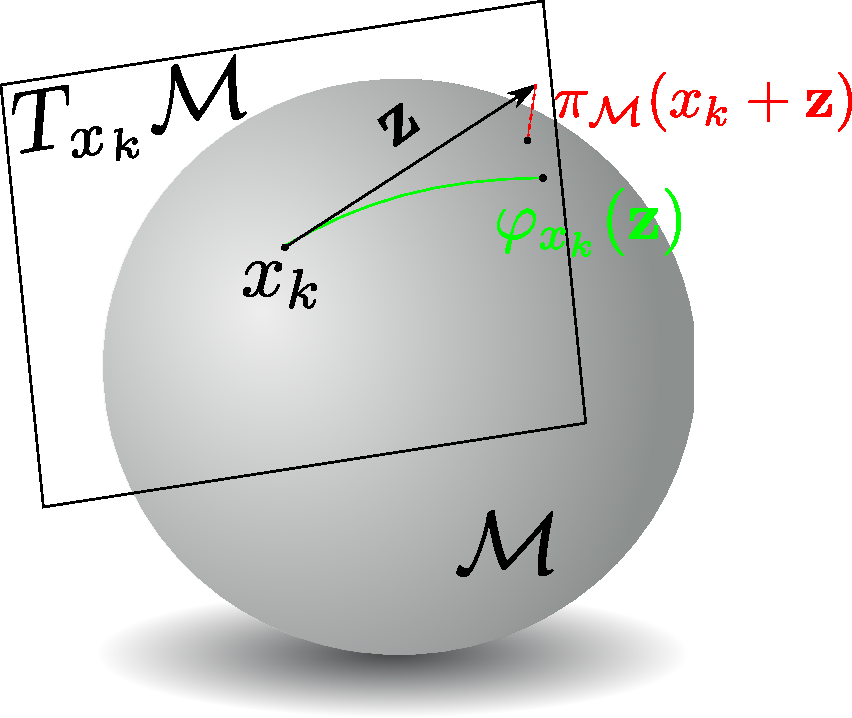
\includegraphics[width=0.5\linewidth]{Humanoids2015/stepOnSphere.pdf}
  %\caption{StepOnSphere}
%\label{fig:stepOnSphere}
%\end{figure}

%As a simple example, the set of 3D-rotations $SO(3)$ is a manifold of dimension $3$.
%The following (classical) choices can be made
%\begin{itemize}
  %\item Rotation matrix ${\bf R} \in \mathbb{R}^{3\times 3} \approx \mathbb{R}^9$, additional constraints: $\{{\bf R}^t{\bf R} = I\ ,\ \det({\bf R})=1\}$, projection by orthogonalization,
  %\item Quaternion ${\bf q} \in \mathbb{R}^4$, additional constraints: $\{ \left\|{\bf q}\right\|=1\}$, projection $\pi({\bf x}) = {\bf x}/\left\|{\bf x}\right\|$,
  %\item Euler angles ($\mathbb{E} = \mathbb{R}^3$), singularities when reaching gimbal lock.
%\end{itemize}

\begin{figure}[htpb]
  \centering
  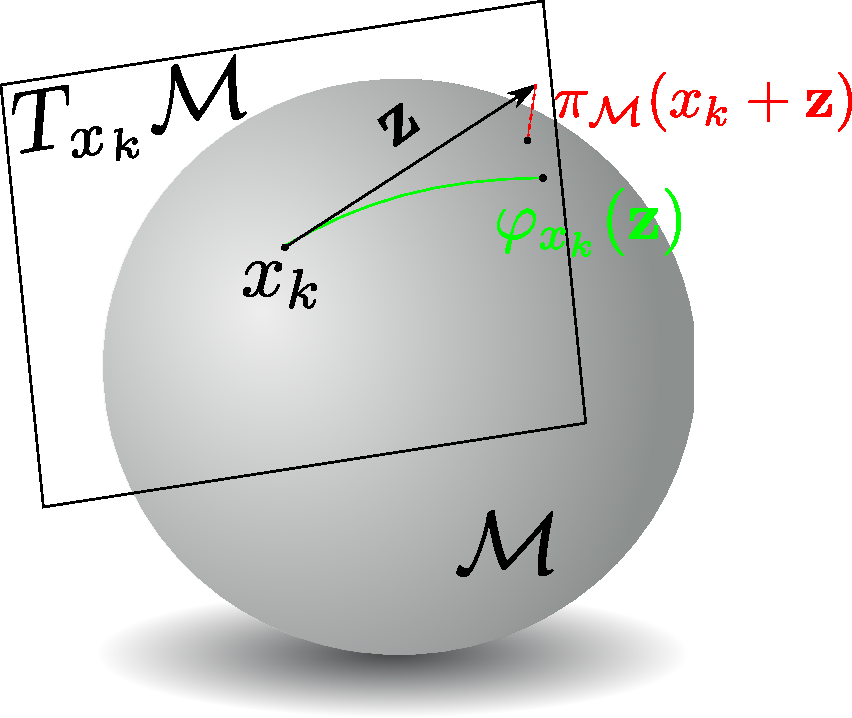
\includegraphics[width=0.5\linewidth]{Humanoids2015/stepOnSphere.pdf}
  \caption{StepOnSphere}
\label{fig:stepOnSphere}
\end{figure}


%}}}
%{{{ LOCAL PARAMETRIZATION
\subsection{Local parametrization}
By definition, there is always, at a point $x$ of a smooth $n$-dimensional manifold $\mathcal{M}$, a smooth function $\varphi_x$ between an open set of $T_x\mathcal{M}$, the tangent space to $\mathcal{M}$ at $x$ (which is isomorphic to $\mathbb{R}^n$), and a neighborhood of $x$ in $\mathcal{M}$, with $\varphi_x(0) = x$.

\begin{equation}
  \varphi_x\ :\
  \begin{array}{ccc}
    \mathbf{z} & \reduce{\mapsto}{6} & \varphi_x(\mathbf{z}) \\
    T_x\mathcal{M} & \reduce{\rightarrow}{6} & \mathcal{M}
  \end{array} \nonumber%
\end{equation}

$\varphi_x$ gives us a local parametrization for $\mathcal{M}$.
Figure~\ref{fig:stepOnSphere} illustrates the difference between a step through $\varphi_x$ in optimization on manifolds and a step followed by a projection $\pi_\mathcal{M}$ as it can be done in classical optimization.

$T_x\mathcal{M}$ can be identified with $\mathbb{R}^n$, but in some cases, it needs to be considered as a hyperplane of a higher dimensionality space.
For example, in figures~\ref{fig:stepOnSphere} and~\ref{fig:phimap}, $T_x\mathcal{M}$ is a 2-dimensional hyperplane embedded in $\mathbb{R}^3$.
We denote $T_x\mathbb{E}$ the representation space of $T_x\mathcal{M}$.
The driving idea of the optimization on manifolds is to change the parametrization of the problem by using a local function $\varphi_{x_i}$ at the current iterate $x_i$ at each iteration.
Applying this idea, we can reformulate Problem~\Eqref{eq:optim_problem} around $x_i$ as:
\begin{align}
\label{eq:local_problem}
\minimize_{{\bf z} \in T_{x_i}\mathcal{M}} & \quad f \circ \varphi_{x_i}({\bf z}) \\
  \text{subject to}&
  \begin{array}{rcl}
    {l} \leq & c \circ \varphi_{x_i}({\bf z}) & \leq {b} \nonumber
  \end{array}
\end{align}
This is an optimization problem on $\mathbb{R}^n$.
If we perform one iteration of a classical solver starting from $x_i$, we compute an increment ${\bf z_i}$, which leads to the next iterate $x_{i+1} = \varphi_{x_i}({\bf z_i})$.
We can then reformulate Problem~\Eqref{eq:optim_problem} around $x_{i+1}$, perform a new iteration and repeat the process until convergence.

\begin{figure}[!htb]
  \centering
  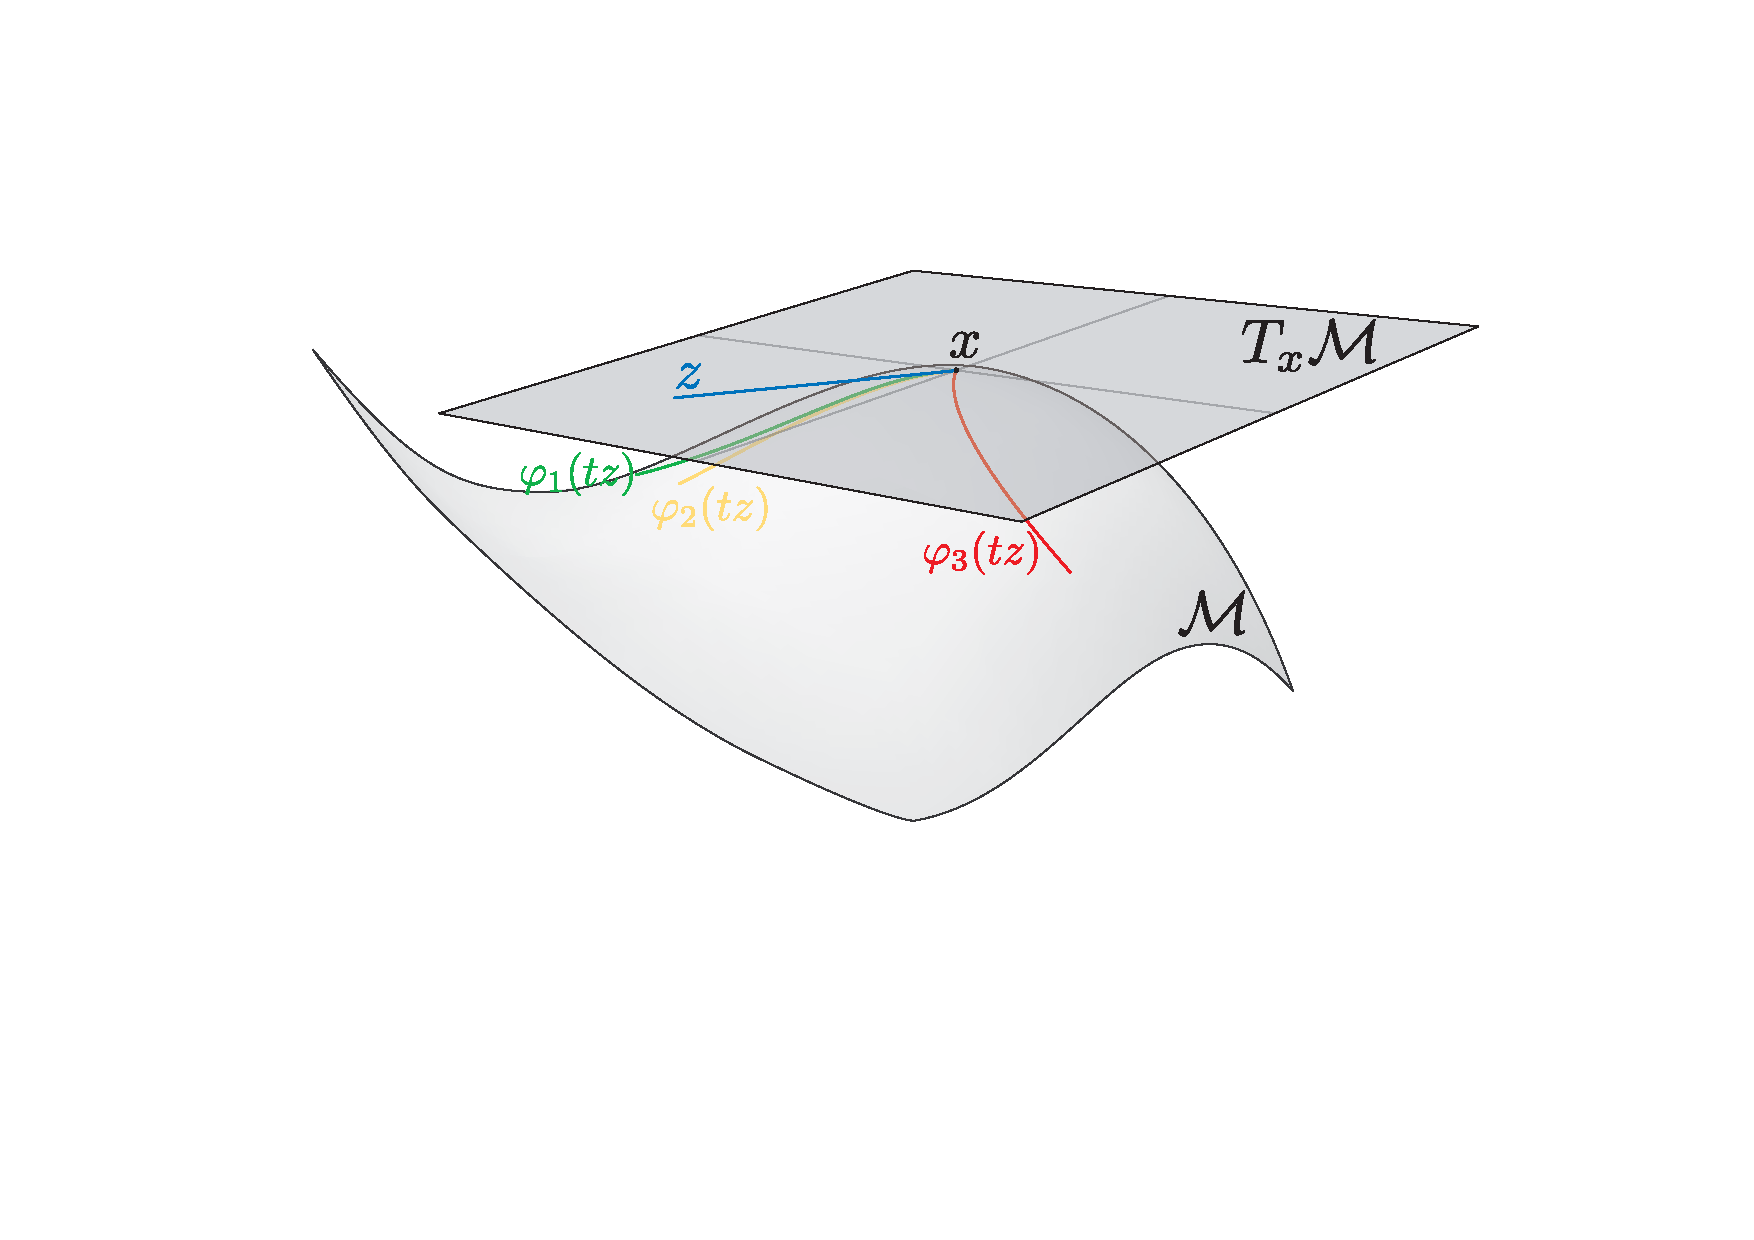
\includegraphics[width=.9\linewidth]{Humanoids2015/manifold.pdf}
  \caption{There are many possible choices for $\varphi_{x}$ but not all yield a curve $\varphi_{x}(t{\bf z})$ which is going in the same direction as ${\bf z}$: $\varphi_{1}$ and $\varphi_{2}$ are correct choices, $\varphi_{3}$ is not.}
\label{fig:phimap}
\end{figure}

However, convergence cannot be achieved without care on the choice of $\varphi_{x_i}$.
Once the optimization algorithm chooses an increment ${\bf z}_i$, we want to move from $x_i$ in the direction of ${\bf z}_i$ on the manifold.
In Euclidean spaces ($\mathbb{R}^n$), moving in the direction of a vector is straightforward.
On a manifold, the notion of moving in the direction of a tangent vector, while staying on the manifold, is generalized by the notion of retractation function.

A retractation $R$ at $x$, denoted $R_x$ is a function from $T_x{\mathcal{M}}$ to $\mathcal{M}$ with a local rigidity condition that preserves gradients at $x$.
Absil~\cite{absil:book:2008} defines a retractation as follows:
\begin{definition}
A retractation on a manifold $\mathcal{M}$ is a smooth function $R$ from the tangent bundle $T\mathcal{M}$ onto $\mathcal{M}$ with the following properties.
Let $R_x$ denote the restriction of $R$ to $T_x\mathcal{M}$.
\begin{enumerate}
  \item $R_x(0_x) = x$, where $0_x$ denotes the zero element of $T_x\mathcal{M}$.
  \item With the canonical identification $T_{0_x}T_x\mathcal{M}\approx T_x\mathcal{M}$, $R_x$ satisfies
  \begin{equation}
    DR_x(0_x) = \mathbf{1}_{T_x\mathcal{M}}
  \end{equation}
  Where $DR_x(0_x)$ denotes the gradient of $R_x$ at $0_x$ and $\mathbf{1}_{T_x\mathcal{M}}$ denotes the identity function on $T_x\mathcal{M}$.
\end{enumerate}
\end{definition}

This means that for any ${\bf z}$, the curve $t \mapsto \varphi_{x_i}(t{\bf z})$ is tangent to ${\bf z}$, see Fig.~\ref{fig:phimap}, so that the update $x_{i+1} = \varphi_{x_i}({\bf z_i})$ is made in the direction given by ${\bf z_i}$.

The exponential map is a good theoretical candidate, but it is often impractical or expensive to compute.
Depending on the manifold, cheaper functions can be chosen such that $\varphi$ is a retractation.

With the iterative formulation approach described above, we do not have any parametrization issue, do not need additional constraints, and have the minimum number of optimization parameters.
We can use the function $\psi:\mathcal{M} \rightarrow \psi(\mathcal{M})$, which is surjective, to represent the $x_i$ and keep track of them in a global way.
%But we still need a map $\psi$ and real space $\mathbb{E}$ to represent the $x_i$ and keep track of them in a global way.
%The ${\bf x_i}$ are guaranteed to be on $\mathcal{M}$ so we can choose a representation with $r>n$ where $\psi$ is singularity-free without any drawback.
Also, the programmer can write the function $f' = f \circ \psi^{-1}$ as if it was a function from $\mathbb{E}$ to $\mathbb{R}$ without the need to project on $\psi(\mathcal{M})$ first (same goes for $c' = c \circ \psi^{-1}$).
For example, if $\mathcal{M} = SO(3)$ and $\mathbb{E} = \mathbb{R}^{3\times 3}$, ${\bf x_i}=\psi(x_i)$ is always a rotation matrix and can be used directly as such when writing the function.

%}}}
%{{{ LOCAL SQP ON MANIFOLDS
\subsection{Local SQP on manifolds}
\label{local_sqp_on_manifolds}

\begin{figure}[htpb]
  \centering
  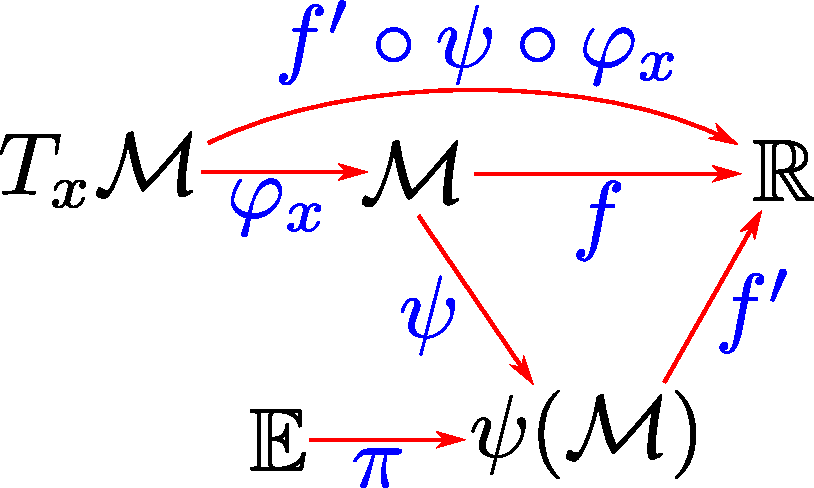
\includegraphics[width=0.5\linewidth]{diagramFunction.pdf}
  \caption{Diagram summarizing the different functions (in blue) and spaces (in black) used to represent a function on a manifold.}
\label{fig:diagram_function}
\end{figure}

We choose to adopt an SQP approach to solve our problem.
We first define the Lagrangian function
\begin{equation}
  %\mathcal{L}_x ({\bf z}, \lambda) = f\circ \varphi_x({\bf z}) - \lambda^T c \circ \varphi_x({\bf z})
  \mathcal{L}_x ({\bf z}, \lambda) = f\circ \varphi_x({\bf z}) - {\lambda_u}^T (c \circ \varphi_x({\bf z}) - u) - {\lambda_l}^T (c \circ \varphi_x({\bf z}) - l)
\end{equation}
with $\lambda_l \in \mathbb{R}^m$ and $\lambda_u \in \mathbb{R}^m$ the vector of Lagrange multipliers respectively associated with the lower and upper bound constraints.
The values of a Lagrange multiplier translate the activity status of the constraint it is associated with (see~\ref{sub:convergence_criterion}).

We denote $H_k$ the Hessian matrix $\nabla_{zz}^2 \mathcal{L}_{x_k}$.
Taking ${\bf z_0} = 0$, the $k$-th SQP step for Problem~\Eqref{eq:local_problem} is computed by solving the following quadratic program:

\begin{align}
  \label{eq:SQPStep}
  \minimize_{\bf z \in \mathbb{R}^n } & \quad {\frac{\partial f\circ \varphi_{x_k}}{\partial {\bf z}}(0)}^T {\bf z } + \frac{1}{2} {\bf z }^T H_k{\bf z }\\
  \text{subject to}&
  \begin{array}{lr}
    \text{l} \leq c\circ \varphi_{x_k}(0) + \frac{\partial c\circ \varphi_{x_k}}{\partial {\bf z}}(0) {\bf z }\leq \text{u}\\
  \end{array} \nonumber%
\end{align}

The basic SQP approach adapted to manifolds can be summarized as follows
\begin{enumerate}
  \item set $k=0$ and $x_k$ to the initial value
  \item compute ${\bf z}$ from Problem~\Eqref{eq:SQPStep} for current $x_k$
  \item set $x_{k+1} = \varphi_{x_k}({\bf z})$ and $k=k+1$
  \item if convergence is not yet achieved go to step 2
\end{enumerate}

Computations of function values and derivatives are based on the fact that $f \circ \varphi = f' \circ \psi \circ \varphi$ (and same for $c$), and
\begin{align}
  f'\ :\
  \begin{array}{ccc}
    \mathbb{E} & \reduce{\rightarrow}{6} & \mathbb{R}
  \end{array} \nonumber\\
  \psi\circ\varphi:
  \begin{array}{ccc}
    T_x{\mathcal{M}} & \reduce{\rightarrow}{6} & \mathbb{E}
  \end{array} \nonumber%
\end{align}
are representable functions (whereas $f$, $\psi$ and $\varphi_x$ are not, due to the fact that they feature $\mathcal{M}$ as input or output).
The gradient of $f \circ \varphi_x$ is
\begin{align}
  \frac{\partial f\circ\varphi_x}{\partial {\bf z}}=
  \frac{\partial f'}{\partial y}(\psi\circ\varphi_x)\times
  \frac{\partial (\psi\circ\varphi_x)}{\partial {\bf z}}
\end{align}

$\frac{\partial f'}{\partial y}$ denotes the gradient of $f'$ with respect to an element of $\mathbb{E}$, which is the derivative that is usually computed for use in classical optimization schemes.

In figure~\ref{fig:diagram_function}, we present a summary of the different functions used in our approach to represent functions on manifolds.

\subsection{Vector transport}
\label{sub:vector_transport}

Nonlinear optimization algorithms such as the SQP rely on the second order information on the problem that is contained in the Hessian.
The exact value the Hessian is not always available, or might be too expensive to compute.
In these cases, we approximate the second order derivative by comparing first order information (tangent vectors) taken on distinct points of the manifold.
Much like in the case of the retractation operation, comparing tangent vectors on a Euclidean space is straightforward, but not on a manifold.

Given $x_1\in\mathcal{M}$ and $\mathbf{z}\in T_{x_1}\mathcal{M}$, we denote $x_2=\varphi_{x_1}(\mathbf{z})$.
We consider two vectors $\mathbf{v}_1 \in T_{x_1}\mathcal{M}$ and $\mathbf{v}_2 \in T_{x_2}\mathcal{M}$ that we want to compare, it is necessary to transport $\mathbf{v}_1$ into $T_{x_2}\mathcal{M}$.

Absil~\cite{absil:book:2008} gives a formal definition of the vector transport in chapter 8.

One can describe the vector transport function from a point $x\in \mathcal{M}$ along an increment $\mathbf{z}$ as:
\begin{equation}
  \mathcal{T}_{x,z} :\
  \begin{array}{ccc}
    \mathbf{v} & \reduce{\mapsto}{6} & \mathcal{T}_{x,\mathbf{z}}(\mathbf{v}) \\
    T_x\mathcal{M} & \reduce{\rightarrow}{6} & T_{\varphi_x(\mathbf{z})}\mathcal{M}
  \end{array} \nonumber%
\end{equation}

%The vector transport can be defined as follows~\cite{absil:book:2008}.

%Let $T\mathcal{M}\oplusT\mathcal{M}=\{(\mathbf{z},\mathbf{v}):\mathbf{z}, \mathbf{v}\in T_x\mathcal{M}, x\in \mathcal{M}$
%\begin{definition}
  %A vector transport on a manifold $\mathcal{M}$ is a smooth mapping
  %\begin{equation}
    %T\mathcal{M}\oplus T\mathcal{M} \rightarrow T\mathcal{M}:(\mathbf{z},\mathbf{v})\mapsto \mathcal{T}_
  %\end{equation}
%\end{definition}

Figure~\ref{fig:transport} illustrates the transport of a vector $\mathbf{v}_1$ from $T_{x_1}\mathcal{M}$ to $T_{x_2}\mathcal{M}$.
%$\mathbf{v}_2$ can then be compared to the transported $\mathbf{v}_1$: $\mathcal{T}_{x_1,\mathbf{z}}(\mathbf{v}_1)$.
%This operation will come in handy for the computation of Hessian approximations explained in Section~\ref{sub:hessian_update_on_manifolds}.

\begin{figure}[htpb]
  \centering
  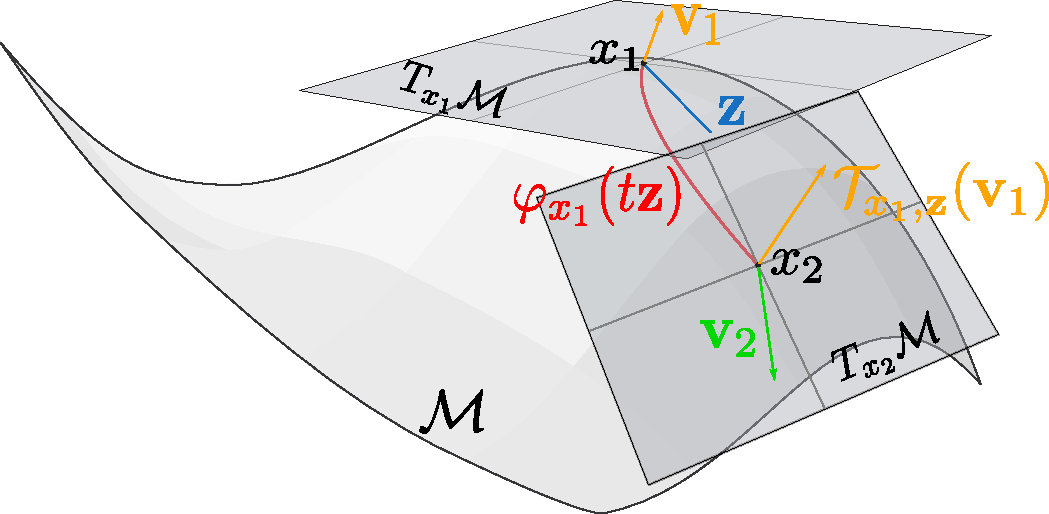
\includegraphics[width=0.8\linewidth]{transport.pdf}
  \caption{Vector transport on a non-Euclidean manifold.}
\label{fig:transport}
\end{figure}


%}}}
%{{{ DESCRIPTION OF NON-EUCLIDEAN MANIFOLDS
\subsection{Description of non-Euclidean manifolds}
\label{sub:examples_on_non_euclidean_manifolds}

In order to develop an optimization algorithm on manifolds, we need to define a set of elements and operations for each elementary manifold $\mathcal{M}$ that will enable us to handle its elements with ease.
%For each elementary manifold $\mathcal{M}$, we need to define a set of elements and operations.
They need to be implemented once only (it is then trivial to get those functions for Cartesian products of manifolds).
The composition with $f'$ and $c'$ is done automatically.
The expression of those functions is adapted from~\cite{boumal:jmlr:2014}.

\paragraph{Retractation:}
We need a retractation operator $\phi_x = \psi\circ\varphi_x$ and its derivative.
During the optimization process, we need the expression of the derivatives of $\phi_x$ in order to compute the gradients of the cost function and of the constraints at the beginning of each iteration.
Because we change the parametrization of our problem to be centered on $x_k$ at each iteration, we only need to evaluate the gradient of $\phi_x$ for $\mathbf{z}=0$, $\frac{\partial \phi_x}{\partial \mathbf{z}}(0)$.
In some cases, this quantity is invariant w.r.t $x$ and can be computed once and for all.

\paragraph{Pseudo-logarithm and distances:}
It is interesting to compute distances on manifolds.
For that, we define the pseudo-logarithm operator (denoted pseudolog), which is the inverse of the retractation operator.
\begin{equation*}
  \zeta_x:\mathcal{M}\rightarrow T_x\mathcal{M}
\end{equation*}
\begin{equation*}
  \forall (x,y)\in \mathcal{M}\times\mathcal{M},\ \mathbf{z}=\zeta_x(y)\ \text{is such that}\ \phi_x(\mathbf{z}) = y
\end{equation*}
The pseudolog operator computes the vector of $T_x\mathcal{M}$ to go from $x$ to $y$.
It is used to compute the (pseudo-) distance between two points of $\mathcal{M}$
\begin{equation*}
  \dist(x,y) = \|\zeta_x(y)\|
\end{equation*}

\paragraph{Vector transport:}
To compare two vectors living in the tangent spaces of different points of $\mathcal{M}$, it is necessary to use the vector transport operation to transport one of them in the space of the other one before comparing them, see Figure~\ref{fig:transport}.
%To compare two vectors of the tangent spaces of $\mathcal{M}$, it is necessary to use the vector transport operation to transport one of them in the space of the other one before comparing them, see Figure~\ref{fig:transport}.
%To compare two vectors $\mathbf{v}_1$ and $\mathbf{v}_2$ defined in tangent spaces of different points, respectively, $T_{x_1}\mathcal{M}$ and $T_{x_2}\mathcal{M}$, it is necessary to transport $\mathbf{v}_1$ into $T_{x_2}\mathcal{M}$.
%Figure~\ref{fig:transport} illustrates the transport of a vector $\mathbf{v}_1$ from $T_{x_1}\mathcal{M}$ to $T_{x_2}\mathcal{M}$.
%$\mathbf{v}_2$ can then be compared to the transported $\mathbf{v}_1$: $\mathcal{T}_{x_1,\mathbf{z}}(\mathbf{v}_1)$.
This operation will come in handy for the computation of Hessian approximations explained later in this chapter.


\paragraph{Projections:} It is useful to define a projection operator on $\mathcal{M}$, as well as one on $T_x\mathcal{M}$, especially to help eliminate some numerical errors when necessary.
The projection operator on $\mathcal{M}$ projects an element of $\mathbb{E}$ onto $\psi(M)\subseteq \mathbb{E}$ while the one on $T_x{M}$ projects an element of $\mathbb{E}$ onto $T_x\mathcal{M}$.

%\paragraph{Limits on tangent map:} The tangent map can present some singularities, thus it is necessary to limit the length of steps made through retractation to the validity region of each manifold.
\paragraph{Limits of validity of the retractation:} The retractation is only valid locally, and we need to give a (conservative) approximation of its validity region.

To summarize, for each elementary manifold $\mathcal{M}$, we need to implement the following elements:
\begin{itemize}
  \item Tangent space at point $x$, $T_x\mathcal{M}$
  \item Embedding spaces $\mathbb{E}$ and $T_x\mathbb{E}$
  \item Retractation operator $\phi:\ (x,\mathbf{z}) \rightarrow \phi_x(\mathbf{z})$
  \item Gradient of the retractation operator at zero $\partial \phi(x):\rightarrow \frac{\partial \phi_x}{\partial \mathbf{z}}(0)$
  \item Pseudo-logarithm operator $\zeta:\ (x,y) \rightarrow \zeta_x(y)$
  \item Gradient of pseudo-logarithm operator at the iterate $\frac{\partial \zeta_x}{\partial y}(x)$
  \item Transport operator $\mathcal{T}:\ (x,\mathbf{z}, \mathbf{v})\rightarrow \mathcal{T}_{x,\mathbf{z}}(v)$
  \item Projection from $\mathbb{E}$ on $\mathcal{M}$, $\pi_\mathcal{M}$
  \item Projection from $T_x\mathbb{E}$ on $T_x\mathcal{M}$, $\pi_{T_x\mathcal{M}}$
  \item Limits of validity of the retractation on $T_x\mathcal{M}$, $\lim$
\end{itemize}

We provide the detailed formulas for those operations in Appendix~\ref{appendix:manifolds} for different elementary manifolds:
\begin{itemize}
  \item The Real space of dimension $n$ in~\ref{sec:the_real_space}
  \item The 3D rotations manifold SO(3) with matrix formulation in~\ref{sec:the_3d_rotation_manifold_matrix_representation}
  \item The 3D rotations manifold SO(3) with quaternion formulation in~\ref{sec:the_3d_rotation_manifold_quaternion_representation}
  \item The unit sphere manifold $S^2$ in~\ref{sec:the_unit_sphere_manifold_s2}
\end{itemize}

%{{{ CARTESIAN PRODUCT OF MANIFOLDS
\subsubsection{Cartesian Product of Manifolds}
\label{ssub:cartesian_product_of_manifolds}
Given two manifolds $\mathcal{M}_1$ and $\mathcal{M}_2$, we denote $\mathcal{M}=\mathcal{M}_1\times\mathcal{M}_2$ their cartesian product.
Any operation on an element of $\mathcal{M}$ can simply be computed term by term for each manifold composing $\mathcal{M}$.
For example, the retractation is computed as follows, and that scheme can be reproduced for all other operations:

\begin{align}
  &x_1\in \mathcal{M}_1,\ \mathbf{z_1}\in T_{x_1}\mathcal{M}_1,\ x_2\in \mathcal{M}_2,\ \mathbf{z_2}\in T_{x_2}\mathcal{M}_2\\
  &x=\begin{bmatrix}
    x_1\\x_2\\
  \end{bmatrix}\in \mathcal{M},\ \mathbf{z}=\begin{bmatrix}
    \mathbf{z_1}\\ \mathbf{z_2}\\
  \end{bmatrix}\in T_x\mathcal{M}\\
  &\phi_x(z) = \begin{bmatrix}
    \phi_{x_1}(\mathbf{z_1})\\
    \phi_{x_2}(\mathbf{z_2})\\
  \end{bmatrix}
\end{align}

%}}}

\subsection{Implementation of Manifolds}
\label{sub:implementation_of_manifolds}

In order to use the manifold formulation described above in other software, and particularly in a numerical solver, we wrote an independent C++ project.
This implementation is open-source and available at \href{https://github.com/stanislas-brossette/manifolds}{https://github.com/stanislas-brossette/manifolds}.
The implementation consists of 3 types of classes: the Manifold class, the elementary manifold classes, and the Point class.
The Manifold class describes the abstract mathematical structure of a non-Euclidean manifold and defines a common interface for all elementary manifolds to implement (retractation, pseudoLog,\ldots).
Elementary Manifold classes ($\mathbb{R}^n$, $SO(3)$, $S^2$, and the Cartesian Product) are the concrete manifolds.
They inherit from the Manifold class and implement all their mathematical operations.
The Cartesian Product class is used to build compound manifolds by being `multiplied' with other elementary manifolds.
The Point class represents a point on a manifold, it contains the data that represents its numerical value.
It can only be constructed by a manifold, and provides some proxy to its manifolds operations.
In particular, it is equipped with an increment method, that applies a retractation on it.
Figure~\ref{fig:uml_manifold} presents a simplified class diagram of this project, omitting all the settor, gettor, bookkeeping mechanics and accessory functions.

\begin{figure}[htpb]
  \centering
  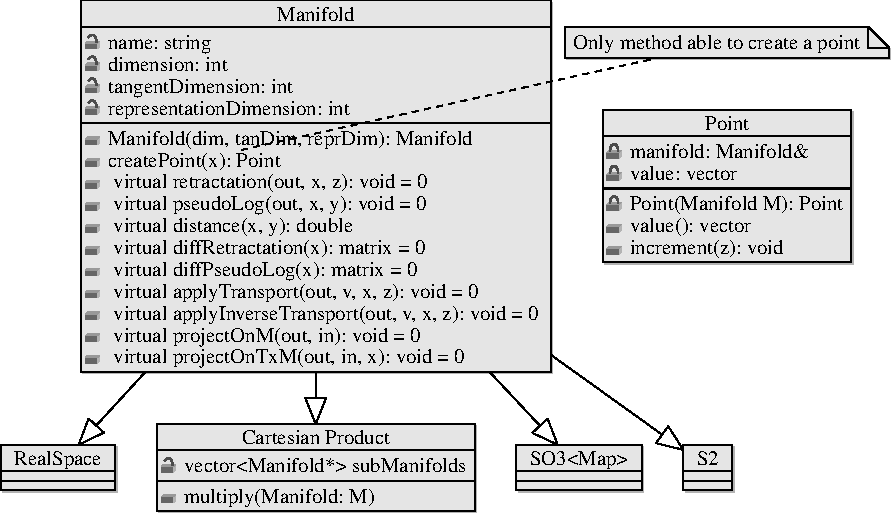
\includegraphics[width=\linewidth]{uml/manifolds-1.pdf}
  \caption{Simplified class diagram of the Manifold project.}
\label{fig:uml_manifold}
\end{figure}

%}}}
%{{{ PRACTICAL IMPLEMENTATION
\section{Practical implementation}
\label{sec:practical_implementation}

The SQP algorithm presented in Section~\ref{local_sqp_on_manifolds} works locally, \emph{i.e.} it is guaranteed to converge when starting close enough to the solution.
In practice, various refinements are made to ensure convergence from any starting point, it is called the globalization.
We detail hereafter the choices we made for the implementation of our solver called {\tt PGSolver}.

We summarize the entire SQP algorithm in Diagrams~\ref{fig:main_sqp_loop},~\ref{fig:restoration_loop} and~\ref{fig:second_order_correction}, which represent respectively the main SQP loop, the restoration phase, and the second order correction algorithm.

\subsection{Linear and quadratic problems resolution}
\label{sub:linear_and_quadratic_problems_resolution}

The central idea of an SQP algorithm is that it solves a series of QP iteratively until a solution is reached.
There are many off-the-shelf QP solvers available and the state of the art is mature in that field.
Thus, we decided to use the {\tt LSSOL} solver~\cite{gill:techrep:1986}.
{\tt LSSOL} provides resolution methods for several types of problems and we are interested in using the resolution methods for FP (Feasibility Problem) and QP.
The {\tt LSSOL} framework formulates problems as follows (Note that there are no equality constraints in this formulation):

\begin{align}
  \minimize_{x\in \mathbb{R}^n}\ &{F(x)}\\
  \text{subject to}\  & l\leq \begin{Bmatrix}
    x\\
    Cx
  \end{Bmatrix}
  \leq u
\end{align}

With the $F$ function taking different forms depending on the problem to solve:
\begin{table} [H]
\centering
\begin{tabular}{ccc}
  \toprule
  FP:\@ & None & (find a feasible point for the constraints)\\
  \midrule
  QP2: & $F(x)=c^T x+\frac{1}{2} x^T A x$ & $A$ symmetric and positive semi-definite \\
  \midrule
  QP4: & $F(x)=c^T x+\frac{1}{2} x^T B^T B x$ & $B$ $m\times n$ upper-trapezoidal \\
  \bottomrule
\end{tabular}
\end{table}

The QP4 type of problem is used when a decomposition of the matrix $A$ of QP2, $A=B^T B$ is already available.

\subsection{Problem Definition}
\label{sub:problem_definition}

As stated in Eq~\Eqref{eq:pb_on_SO3} we want to solve a nonlinear constrained optimization problem on manifold that takes the following form:

\begin{align}
  \minimize_{x \in \mathcal{M}} & \quad f(x)\\
  \text{subject to}&
  \begin{array}{lr}
    l \leq c(x) \leq u \nonumber
  \end{array}
\end{align}

The list of constraints can be separated into 3 categories: Bounds, Linear, and Nonlinear.
For convenience, we formulate our optimization problem in a way that is compatible with {\tt LSSOL} by changing all equality constraints into inequality constraints:

\begin{equation}
  c(x) = a \Leftrightarrow a \leq c(x) \leq a
\end{equation}

Our problem can be written as:
\begin{align}
\label{eq:optim_problem_on_manifold}
  \minimize_{x \in \mathcal{M}} & \quad f(x)\\ \nonumber
  \text{subject to}&\left\{
  \begin{array}{lr}
    L_B \leq x \leq U_B \\
    L_L \leq Ax \leq U_L \\
    L_N \leq c(x) \leq U_N
  \end{array}\right.
\end{align}

With $L_B$ and $U_B$ being respectively the lower and upper bounds for Bounds constraints, $L_L$ and $U_L$ the lower and upper bounds for Linear constraints, and $L_N$ and $U_N$ the lower and upper bounds for Nonlinear constraints.
That formulation is conveniently used to define our problem.
Since we are solving this problem on a non-Euclidean manifold, we need to re-formulate it around the current iterate $x_i$ at each iteration.
This is done automatically behind the scene and the user only has to provide the information to build problem~\Eqref{eq:optim_problem_on_manifold}.

At iteration $i$, the problem becomes (for clarity, we drop the subscript $i$ that goes with each appearance of $x$):
\begin{align}
\label{eq:optim_problem_on_txm}
  \minimize_{\mathbf{z} \in T_x\mathcal{M}} & \quad f(\phi_x(\mathbf{z}))\\ \nonumber
  \text{subject to}&\left\{
  \begin{array}{lr}
    {\bf z}_{\text{map}}^- \leq \mathbf{z} \leq {\bf z}_{\text{map}}^+ \\
    L_B \leq \phi_x(\mathbf{z}) \leq U_B \\
    L_L \leq A\phi_x(\mathbf{z}) \leq U_L \\
    L_N \leq c(\phi_x(\mathbf{z})) \leq U_N \\
  \end{array}\right.
\end{align}

With ${\bf z}_{\text{map}}^-$ and ${\bf z}_{\text{map}}^+$ being respectively the lower and upper bounds of validity of the tangent map of $\mathcal{M}$ around $x$.
After this reformulation, we note that if $\phi_x$ is nonlinear, then the bounds and linear constraints of problem~\Eqref{eq:optim_problem_on_manifold} become nonlinear in problem~\Eqref{eq:optim_problem_on_txm}.
It is then necessary to treat the problem and evaluate which constraint is linear and which is not, in order to go back to a formulation of the same type as in problem~\Eqref{eq:optim_problem_on_manifold}.
Basically, for each constraint $c_j$ in problem~\Eqref{eq:optim_problem_on_txm}, if the submanifold of $\mathcal{M}$ on which that constraint is applied is a real space $\mathbb{R}^m$ then the constraint maintains its bound, linearity or nonlinearity status, otherwise, it becomes a nonlinear constraint\footnote{This treatment of the constraints is a planned work, it has not been implemented yet.}.
It is, however, unusual to write linear constraints on non-Euclidean manifolds.
%Once again, this may look like a drawback of optimization on manifolds, but it is usually the same with classical optimization.
%Indeed, a linear constraint on the representation space of a non-Euclidean manifold might not often make much sense.
%For example, a linear constraint on the elements of a unit quaternion, although one can obviously be devised, does not seem to make much sense.
%So usually, when a non-Euclidean manifold is involved, the constraint is nonlinear.

In the particular case of linear constraints (and by extension bound constraints) on a submanifold that is a real space, the constraints on $x$ are transformed into constraints on $z$ as follows:
\begin{equation}
  L_L \leq Ax \leq U_L \ \Rightarrow \ L_L - Ax \leq A\mathbf{z} \leq U_L-Ax
\end{equation}
For bounds constraints, the same goes with $A$ being the identity matrix on the submanifold.

Once those substitutions are done, we obtain a new problem of the following form (where $L_B'$, $L_L'$, $L_N'$, $U_B'$, $U_L'$, $U_N'$ are the lower and upper bounds for the bounds, linear and nonlinear constraint, $A'$ is the matrix of linear constraints and $c'$ is the list of nonlinear functions):

\begin{align}
\label{eq:optim_txm_final}
  \minimize_{\mathbf{z} \in T_x\mathcal{M}} & \quad f \circ \phi_x(\mathbf{z})\\ \nonumber
  \text{subject to}&\left\{
  \begin{array}{lr}
    L_B' \leq \mathbf{z} \leq U_B' \\
    L_L' \leq A' \mathbf{z} \leq U_L' \\
    L_N' \leq c' \circ \phi_x(\mathbf{z}) \leq U_N'\\
  \end{array}\right.
\end{align}

This problem is an exact reformulation of problem~\Eqref{eq:optim_problem_on_manifold} on $T_x\mathcal{M}$.
At each step of the optimization process, we solve the QP approximating this problem~\Eqref{eq:optim_txm_final} around $\mathbf{z}=0$.
The Taylor development of $c\circ\phi_x(z)$ to the first order around $\mathbf{z} = 0$ gives:
\begin{equation}
  c' \circ \phi_x(\mathbf{z}) \approx c'\circ \phi_{x_k}(0) + \frac{\partial c'\circ \phi_{x_k}}{\partial {\bf z}}(0) {\bf z } = c'(x_k) + {\left(\nabla\phi_{x_k}(0) \nabla c' (x_k)\right)}^T\mathbf{z}
\end{equation}

The trust-region constraint (see Section~\ref{sub:trust_region_and_limit_map}) is added to the problem to limit the length of a step, $\rho$ denotes the size of the trust-region.
$H_k$ is an estimation of the Hessian computed as shown in Section~\ref{sub:hessian_update_on_manifolds}.
The QP to be solved at each iteration is the following:

\begin{align}
  \label{eq:QP_txm}
  \begin{split}
  \minimize_{\mathbf{z} \in T_x\mathcal{M}=\mathbb{R}^n } & \quad {\left(\nabla\phi_{x_k}(0) \nabla f (x_k)\right)}^T\mathbf{z} + \frac{1}{2} {\bf z }^T H_k{\bf z }\\
  \text{subject to}&\left\{
  \begin{array}{lr}
    L_B' \leq \mathbf{z} \leq U_B' \\
    L_L' \leq A' \mathbf{z} \leq U_L' \\
    L_N' \leq c'(x_k) + {\left(\nabla\phi_{x_k}(0) \nabla c' (x_k)\right)}^T\mathbf{z}\leq U_N'\\
    -\rho \leq \mathbf{z} \leq \rho \quad (\text{trust-region constraint}) \\
  \end{array}\right.
  \end{split}
\end{align}

The resolution of this QP~\Eqref{eq:QP_txm} (with {\tt LSSOL}) gives the optimal solution $\mathbf{z}^*$ and Lagrange multipliers $\lambda^*$.
The new iterate that will be considered is:
\begin{align}
  x_{k+1} & \leftarrow \phi_{x_k}(\mathbf{z}^*)\\
  \lambda_{k+1} & \leftarrow \lambda^*
\end{align}

Note that the only additional computation due to the formulation on manifolds is the multiplication of the gradients of constraints and cost by the map's gradient at $0$.
The computation time related to those products can be reduced by taking advantage of the fact that $\nabla \phi_x(0)$ is block-diagonal.

\subsection{Trust-region and limit map}
\label{sub:trust_region_and_limit_map}

Maps $\varphi_{x}$ are only valid locally, and we need to be aware of this fact: a step ${\bf z}$ found by solving Problem~\Eqref{eq:QP_txm} should not be outside the validity region of the map.
This can be enforced by adding the limits of the manifold map to the problem as bound constraints.
In fact, this can be done by intersecting the original problem's bounds with the limits of the map and imposing the resulting bounds as constraints.
This leads naturally to trust region methods that we, therefore, favor over line-search approaches.
We present the classical trust-region strategy in Section~\ref{ssub:the_trust_region_strategy}.

In the case of a robotics problem, different variables often have different orders of magnitude, for example, contact forces can be of the order of hundreds of Newtons, depending on the weight and torque capacity of the robot, while joint angles are of the order of radians.
Let $x$ be the variable vector of such problem with $x={[\theta_0, \theta_1, f_0, f_1, f_2]}^T$ where $\theta_i$ represent angular variables and $f_i$ forces.
The shape of the trust-region should reflect those differences, but we want to keep the simplicity of the classical trust-region strategy.
For that, we propose to separate the trust-region $\rho$ in two parts: its scale $\rho_\text{scale}$ which is a scalar, and its shape $\rho_\text{shape}$ which in a vector of dimension $n$ (that value is actually stored in the instance of manifold).
$\rho_\text{shape}$ is constant and set at the beginning of the optimization, the i-th element of $\rho_\text{shape}$ is the order of magnitude of the i-th dimension of the optimization variable.
In the previous example, we'd get ${\rho_\text{shape}} = {[1,1,100,100,100]}^T$
And $\rho_\text{scale}$ is the scalar that gets updated in the trust-region strategy.

Finally, the constraints related to the trust-region added to the problem is:
\begin{equation}
  -\rho = -\rho_\text{scale}\rho_\text{shape} \leq \mathbf{z} \leq \rho_\text{scale}\rho_\text{shape} = \rho
\end{equation}

\subsection{Filter method}
\label{sub:filter_method}

To know if a step ${\bf z}$ is acceptable or not, one usually uses a penalty-based merit function as we present in Section~\ref{sec:resolution_of_a_non_linear_constrained_optimization_problem}.
In our early tests, the update of the penalty parameters proved to be difficult with our types of problems.
We now use a filter approach instead, as presented in Section~\ref{ssub:the_filter_method}.

Our algorithm is an adaptation of Fletcher's filter SQP~\cite{fletcher:mathprog:2000} to the case of manifolds: we use an adaptive trust-region that is intersected with the validity region of $\phi_{x_i}$, and a new iterate $x_{i+1} = \phi_{x_i}({\bf z})$ is accepted if either the cost function or the sum of constraint violations is made better than for any previous iterates.

\subsection{Convergence criterion}
\label{sub:convergence_criterion}

An iterate $\{x,\lambda\}$ is considered to be a solution of the optimization problem if it satisfies the first-order optimality conditions (presented in Section~\ref{sub:optimality_conditions}) to within certain tolerances.
We use the same criterion as the one used in \href{http://www.sbsi-sol-optimize.com/asp/sol_product_snopt.htm}{{\tt SNOPT}} and presented in~\cite{gill:snopt:2002}.
It has the advantage of using two different tolerance constants: $\tau_P$ monitors the primal optimality conditions, which means the satisfaction of the constraints, and $\tau_D$ monitors the dual conditions, which means the optimality of the cost function and of the Lagrange multipliers.
That gives the user more control over the quality of the solution.

Dropping the distinction between Linear and Nonlinear Constraints,
the problem can be rewritten as:

\begin{align}
\begin{split}
\label{eq:problem}
  \minimize_{\bf x \in \mathcal{M}} & \quad \mbox{\emph{f}}({\bf x}) \\
  \text{subject to }&
  l \leq c({\bf x}) \leq u \\
\end{split}
\end{align}

Each constraint is considered as a double inequality, thus, is associated with two Lagrange multipliers: $\lambda_l$ for the lower bound and $\lambda_u$ for the upper bound.
The basic KKT condition for this problem writes as:

\begin{equation}
\label{KKT}
\left\{
\begin{array}{lr}
  \nabla \mathcal{L} = \nabla f({\bf x}) + \lambda_l.\nabla c({\bf x}) + \lambda_u.\nabla
c({\bf x}) = 0 \\
  \forall i
  \begin{cases}
  c_i({\bf x}) - l_i \geq 0 \\
  c_i({\bf x}) - u_i \leq 0 \\
  {\lambda_l}_i \leq 0 \\
  {\lambda_u}_i \geq 0 \\
  {\lambda_l}_i.(c_i({\bf x})-l_i) = 0 \\
  {\lambda_u}_i.(c_i({\bf x})-u_i) = 0
  \end{cases}
\end{array}
\right.
\end{equation}

For each constraint, there are 3 possible situations:

\begin{tabular}{cccc}
  \\ \toprule
  Lower bound violated or active & $c_i(x)-l_i\leq0$ & ${\lambda_l}_i\leq0$ & ${\lambda_u}_i=0$ \\
  \midrule
  Constraint satisfied & $l_i\leq c_i(x) \leq u_i$ & ${\lambda_l}_i=0$ & ${\lambda_u}_i=0$ \\
  \midrule
  Upper bound violated or active & $c_i(x)-u_i\geq0$ & ${\lambda_l}_i=0$ & ${\lambda_u}_i\geq0$ \\
  \bottomrule \\
\end{tabular}

Both $\lambda_l$ and $\lambda_u$ cannot be nonzero at the same time.
So for each constraint, we can use a single Lagrange multiplier that is negative when the lower bound is violated or active, null when the constraint is satisfied, and positive when the upper bound is active or violated.
This allows to reduce the KKT system to the following:

\begin{equation}
\label{KKTmodified}
\left\{
\begin{array}{lr}
  \nabla \mathcal{L} = \nabla f({\bf x}) + \lambda.\nabla c({\bf x}) = 0 \\
  \forall i
  \begin{cases}
  c_i({\bf x}) = l_i & \text{and } \lambda_i \leq 0 \\
  \text{OR}\\
  l_i \leq c_i({\bf x}) \leq u_i & \text{and } \lambda_i = 0 \\
  \text{OR}\\
  c_i({\bf x}) = u_i & \text{and } \lambda_i \geq 0
  \end{cases}
\end{array}
\right.
\end{equation}

To evaluate the satisfaction of this system, we approximate it with the tolerance constants.
First, we scale the tolerance constants with respect to the values of the iterate $x$ and $\lambda$:
\begin{align}
\begin{split}
  \tau_x = \tau_P(1+\|x\|_\infty)\\
  \tau_\lambda =\tau_D(1+\|\lambda\|_\infty)\\
\end{split}
\end{align}

And we get the following convergence criterion:
\begin{equation}
\label{KKTfinal}
\left\{
\begin{array}{lr}
  \|\nabla \mathcal{L}\|_\infty \leq \tau_\lambda \\
  \forall i\
  \left\{
  \begin{array}{lll}
  |c_i({\bf x}) - l_i| \leq \tau_x & \text{and } \lambda_i \leq -\tau_\lambda\\
  \text{OR}\\
  -(c_i({\bf x}) - l_i) \leq -\tau_x &\text{and } -(c_i({\bf x}) - u_i) \geq -\tau_x & \text{and } |\lambda| \leq \tau_\lambda \\
  \text{OR}\\
  |c_i({\bf x}) - u_i| \leq \tau_x & \text{and } \lambda_i \geq \tau_\lambda\\
  \end{array}
  \right.
\end{array}
\right.
\end{equation}

\subsection{Feasibility restoration}
\label{sub:feasibility_restoration}

During the optimization process, the set of linearized constraints in the QP Problem~\Eqref{eq:QP_txm} can become unfeasible, for example after a reduction of the trust-region, see Section~\ref{ssub:the_trust_region_strategy}.
In such a case, the QP~\Eqref{eq:QP_txm} cannot be solved and the resolution as presented above cannot proceed.
To cope with this issue, the algorithm enters the so-called restoration phase, which aims at finding a feasible point without regards for the value of the cost function.
The basic idea is the following: at the beginning of an iteration, the list of unfeasible constraints is computed and stored in $\mathcal{U}_l$ if the lower bound is unfeasible, and in $\mathcal{U}_u$ if the upper bound is unfeasible, and the list of feasible constraints is stored in $\mathcal{F}$.
The unfeasible constraints are removed from the restoration problems' constraints list and their violation is added to its cost function (that becomes the sum of all constraints violation).
We get the following restoration cost function:
\begin{equation}
  f^\text{rest} = \sum_{i\in\mathcal{U}_l} (l_i - c_i(x)) +\sum_{i\in\mathcal{U}_u} (c_i(x) - u_i)
\end{equation}
Then the restoration problem only contains feasible constraints and has to minimize the sum of constraint violation.
The problem to solve becomes:
\begin{align}
\label{eq:restoration_problem}
  \minimize_{x \in \mathcal{M}} & \quad \sum_{i\in\mathcal{U}_l} (l_i - c_i(x)) +\sum_{i\in\mathcal{U}_u} (c_i(x) - u_i)\\ \nonumber
  \text{s.t.}&\left\{
  \begin{array}{lr}
    \forall i \in \mathcal{F}   \quad l_i \leq c_i(x) \leq u_i \\
    \forall i \in \mathcal{U}_l \quad -\infty \leq c_i(x) \leq u_i \\
    \forall i \in \mathcal{U}_u \quad l_i \leq c_i(x) \leq +\infty \\
  \end{array}\right.
\end{align}
To simplify the writing of that QP, we denote $l^\text{rest}$ and $u^\text{rest}$ two vectors that represent respectively the lower and upper bounds of the constraints of the restoration problem:
\begin{align}
  \forall i \in \mathcal{F}   ,\ & l^\text{rest}_i = l_i    ,\ u^\text{rest}_i = u_i \\
  \forall i \in \mathcal{U}_l ,\ & l^\text{rest}_i = -\infty,\ u^\text{rest}_i = u_i \\
  \forall i \in \mathcal{U}_u ,\ & l^\text{rest}_i = l_i    ,\ u^\text{rest}_i = +\infty \\
\end{align}

The problem becomes:
\begin{align}
\label{eq:restoration_problem_simple}
  \minimize_{x \in \mathcal{M}} & \quad \sum_{i\in\mathcal{U}_l} (l_i - c_i(x)) +\sum_{i\in\mathcal{U}_u} (c_i(x) - u_i)\\ \nonumber
  \text{s.t.}&\left\{
  \begin{array}{lr}
    \forall i \quad l^\text{rest}_i \leq c_i(x) \leq u^\text{rest}_i \\
  \end{array}\right.
\end{align}


That is solved by iterating just like in the SQPs main loop with the difference that at each iteration, we update the problem based on new lists of unfeasible constraints.
An approximation $H^\text{rest}_k$ of the Hessian is computed especially for the restoration phase.
The restoration phase has and updates its own trust-region $\rho_\text{rest}$.
Dropping the differences between bounds, linear and nonlinear constraints, the QP to solve at each iteration of the restoration phase is the following:
\begin{align}
  \label{eq:QP_restoration}
  \begin{split}
  \minimize_{\mathbf{z} \in T_x\mathcal{M} } & \quad {\left(\nabla\phi_{x_k}(0) \nabla f^\text{rest} (x_k)\right)}^T\mathbf{z} + \frac{1}{2} {\bf z }^T H^\text{rest}_k{\bf z }\\
  \text{s.t.}&\left\{
  \begin{array}{lr}
    \forall i \quad l^\text{rest}_i \leq c_i(x_k) + {\left(\nabla\phi_{x_k}(0) \nabla c_i (x_k)\right)}^T\mathbf{z} \leq u^\text{rest}_i \\
    -\rho^\text{rest} \leq \mathbf{z} \leq \rho^\text{rest} \\
  \end{array}\right.
  \end{split}
\end{align}


The restoration phase has its own filter called the restoration filter.
For more details on the restoration phase, see Section~\ref{sub:restoration_phase}.

Note that each iteration of the main SQP algorithm starts with the resolution of an FP (Feasibility Problem), that consists of the same linearized constraints as the QP problem~\Eqref{eq:QP_txm} without the cost function.
\begin{align}
  \label{eq:FP_txm}
  \begin{split}
  \text{find } \mathbf{z}\ \text{such that:}&\left\{
  \begin{array}{lr}
    L_B \leq \mathbf{z} \leq U_B \\
    L_L \leq A \mathbf{z} \leq U_L \\
    L_N \leq c(x_k) + {\left(\nabla\phi_{x_k}(0) \nabla c_i (x_k)\right)}^T\mathbf{z}\leq U_N\\
  \end{array}\right.
  \end{split}
\end{align}

Its role is to determine whether the set of linearized constraints is feasible.
If it is, the main SQP continues, otherwise, the restoration phase is entered.
This feasibility problem is also solved at the beginning of each restoration iteration to determine whether or not to exit the restoration phase.
As soon as a feasible point is found, the restoration process ends.
Once a feasible point $x_F$ is found by the restoration phase, it is used as the new iterate in the main SQP phase.
Since during the restoration no care is taken about the value of the cost function, it is possible that $x_F$ is refused by the main filter, which is not an acceptable behavior.
So $x_F$ is forced in the filter, and any pair dominating it is removed.
Then the main phase of the optimization can continue.

\subsection{Second Order Correction}
\label{sub:second_order_correction}

In the event where a step proposed in the restoration process by the resolution of the restoration QP is rejected by the restoration filter, instead of immediately reducing the size of the trust region, we can perform a Second Order Correction Step.

The idea is to re-solve a QP after its solution $\mathbf{z}_k$ has been rejected by the restoration filter, but with a better approximation (second order) of the constraints:
\begin{equation}
  c_i(x_k+{\bf z}) = c_i(x_k) + {\nabla c_i(x_k)}^T {\bf z} + \frac{1}{2}{\bf z}^T{\nabla}^2c_i(x_k){\bf z}
\end{equation}

The restoration QP problem becomes:
\begin{align}
  \label{eq:QP_soc_dirty}
  \begin{split}
  \minimize_{\mathbf{z} \in T_x\mathcal{M} } & \quad {\left(\nabla\phi_{x_k}(0) \nabla f^\text{rest} (x_k)\right)}^T\mathbf{z} + \frac{1}{2} {\bf z }^T H^\text{rest}_k{\bf z }\\
  \text{s.t.}&\left\{
  \begin{array}{lr}
    \forall i \quad l^\text{rest}_i \leq c_i(x_k) + {\left(\nabla\phi_{x_k}(0) \nabla c_i (x_k)\right)}^T\mathbf{z} + \frac{1}{2}{\bf z}^T{\nabla}^2c_i(x_k){\bf z}
 \leq u^\text{rest}_i \\
    -\rho^\text{rest} \leq \mathbf{z} \leq \rho^\text{rest} \\
  \end{array}\right.
  \end{split}
\end{align}

Using $ \frac{1}{2}{\bf z}^T{\nabla}^2c_i(x_k){\bf z} \approx c_i(x_k+{\bf z}_k) - c_i(x_k) - {\nabla c_i(x_k)}^T {\bf z}_k $
we get:
\begin{align}
  \label{eq:QP_soc}
  \begin{split}
  \minimize_{\mathbf{z} \in T_x\mathcal{M} } &\quad {\left(\nabla\phi_{x_k}(0) \nabla f^\text{rest} (x_k)\right)}^T\mathbf{z} + \frac{1}{2} {\bf z }^T H^\text{rest}_k{\bf z }\\
  \text{s.t.}&\left\{
  \begin{array}{lr}
    \forall i \quad l^\text{rest}_i \leq {\left(\nabla\phi_{x_k}(0) \nabla c_i (x_k)\right)}^T(\mathbf{z} - \mathbf{z}_k) + c_i(\phi_{x_k}({\bf z}_k)) \leq u^\text{rest}_i \\
    -\rho^\text{rest} \leq \mathbf{z} \leq \rho^\text{rest} \\
  \end{array}\right.
  \end{split}
\end{align}

Denoting $g_k = {\left(\nabla\phi_{x_k}(0) \nabla f (x_k)\right)}$ and $A_k = {\left(\nabla\phi_{x_k}(0) \nabla c_i (x_k)\right)}$, we can rewrite~\ref{eq:QP_soc} as follows:
\begin{align}
  \label{eq:QP_soc_simple}
  \begin{split}
  \minimize_{\mathbf{z} \in T_x\mathcal{M} }& \quad g_k^T\mathbf{z} + \frac{1}{2} {\bf z }^T H^\text{rest}_k{\bf z }\\
  \text{s.t.}&\left\{
  \begin{array}{lr}
    \forall i \quad l^\text{rest}_i + A_k\mathbf{z}_k - c_i(\phi_{x_k}({\bf z}_k)) \leq A_k^T\mathbf{z}\leq u^\text{rest}_i+ A_k\mathbf{z}_k - c_i(\phi_{x_k}({\bf z}_k))  \\
    -\rho^\text{rest} \leq \mathbf{z} \leq \rho^\text{rest} \\
  \end{array}\right.
  \end{split}
\end{align}

This system is solved iteratively by updating $\mathbf{z}_k$ (but never changing $x$) with the solution of the previous system and updating the values of $c_i(\phi_{x_k}(\mathbf{z}_k))$ until a satisfactory $\bf z$ is found.

\subsection{Hessian update on manifolds}
\label{sub:hessian_update_on_manifolds}

Aside from the manifold adaptation, our main departure from Fletcher is in the Hessian computation, where we used an approximation because the exact Hessian is too expensive to compute in our problems.
After testing several possibilities, we settled for a self-scaling damped BFGS update~\cite{nocedal:mp:1993,nocedal:book:2006}, adapted to the manifold framework.
More precisely, given the Hessian approximation $H_k$ at iteration $k$, we compute the approximation $H_{k+1}$ as follows:
Note that as explained in Section~\ref{sub:vector_transport}, the gradients are transformed through vector transport before being compared.
\begin{align}
  &s_k = \mathcal{T}_{\bf z}(z), \quad y_k = \nabla_z \mathcal{L}_{x_{k+1}}(0,\lambda_{k+1}) - \mathcal{T}_{\bf z}(\mathcal{L}_{x_{k}}(0,\lambda_{k})) \nonumber\\
  &\theta_k = \left\{\begin{array}{ll}
    1 & \mbox{if} \; s_k^T y_k \geq 0.2 s_k^T \tilde{H}_k s_k \\
    \frac{0.8 s_k^T \tilde{H}_k s_k}{s_k^T \tilde{H}_k s_k - s_k^T y_k} & \mbox{otherwise}
  \end{array}\right. \quad \mbox{(Powell update)}\nonumber\\
  &r_k = \theta_k y_k + \left(1-\theta_k\right) \tilde{H}_k s_k \quad \mbox{(damped update)} \nonumber\\
  &\tau_k = \min\left(1, \frac{s_k^T r_k}{s_k^T \tilde{H}_k s_k} \right) \quad \mbox{(self-scaling)} \nonumber\\
  &H_{k+1} = \tau_k \left(\tilde{H}_k-\frac{\tilde{H}_k s_k s_k^T \tilde{H}_k}{s_k^T \tilde{H}_k s_k} \right) + \frac{r_k r_k^T}{s_k^T r_k} \nonumber%
\end{align}
where $\mathcal{T}_{\bf z}$ is a vector transport along ${\bf z}$ (see~\cite{absil:book:2008}) and $\tilde{H}_k$ is such that for ${\bf u} \in T_{x_{k+1}} \mathcal{M}$, $\tilde{H}_k {\bf u} = \mathcal{T}_{\bf z}\left(H_k \mathcal{T}_{\bf z}^{-1}({\bf u}) \right)$.

\subsection{Hessian Regularization}
\label{sub:hessian_regularization}

Despite Powell's update, $H_{k}$ might not be positive definite (but still symmetric).
We regularize it as follows: we first perform a Bunch-Kaufman factorization $P_k H_k P_k^T= L_k B_k L_k^T$ where $P_k$ is a permutation matrix, $L_k$ is unit lower triangular and $B_k$ is block diagonal with blocks of size $1 \times 1$ or $2\times 2$ (obtaining $B_k$ as a diagonal matrix is not numerically stable for Cholesky-like decomposition of indefinite matrices), see~\cite{golub:book:1996}.
The eigenvalue decomposition $B_k = Q_k D_k Q_k^T$ is immediate and cheap to compute.
From the diagonal matrix $D_k$, we form $D'_k$ such that $d'_{ii} = \max\left(d_{ii},\mu_{\min}\right)$ where $\mu_{\min}>0$ is user-defined (we typically set it to $0.1$).
Defining $L'_k = L_k Q_k {(D'_k)}^{1/2}$, we get a regularized matrix $H'_k = P_k^T L_k L_k^T P_k = (L_k^T P_k)^T L_k^T P_k$.
%In our case, we use {\tt LSSOL}~\cite{gill:techrep:1986} for solving the QP~\Eqref{eq:SQPStep}, which directly accepts the factorized form $(P_k, L'_k)$.
We take advantage of {\tt LSSOL}'s capability to receive $H$ in the factorized form $H=A^TA$ with $A=L_k^T P_k$ upper-trapezoidal as an input.
This avoids an internal Cholesky factorization so that our regularization does not add too much time to the overall process of building and solving the QP.\@

\subsection{An alternative Hessian Approximation Update}
\label{sub:an_alternative_hessian_approximation_update}

In~\cite{Fletcher:ifip:2006}, Fletcher presents a new Hessian update method that maintains and update the Hessian $H$ in the form $H=U U^T$, which is obviously always symmetric and it ensures that it is always positive semi-definite.
Since a decomposition of $H$ is readily available with this method, we can get rid of the regularization of the Hessian in our algorithm.
The matrix $U$ of size $(n,m)$ is smaller than $H$ and contains only information from the last $m$ iteration, this means that this method has a built-in limited memory capability.
In our robotics problems, using limited memory Hessian updates is useful because along the iteration process, the variables may change a lot, and the Hessian value near the solution may be very different from the one approximated around the first iterations.
Thus, it can be helpful to `forget' about the old components of the approximation to leave room for the latest ones.
At each iteration, the matrix $U$ is updated with either BFGS or SR1, or a hybrid method, based on some tests on the value of the latest step.
When possible, the SR1 update is preferred, because some results suggest that it allows faster convergence when the SR1 denominator is positive, otherwise, a BFGS or the hybrid method are used.

Although this method provides a decomposition of $H$ as $U U^T$, $U$ is not trapezoidal, so we need to apply a QR on $U^T$ so that we get $U^T=QR$, then $H=R^T Q^T Q R=Q^T Q$ with Q trapezoidal and R an orthogonal matrix.
Then $Q$ can be fed to {\tt LSSOL} directly.

For all those reasons, this update method is very attractive.
We implemented it in our solver, but so far the results have not been very conclusive and some more work will be dedicated to that issue in the future.
As of now, the best results were observed when using the self-scaling BFGS update method.

\subsection{Hessian Update in Restoration phase}
\label{sub:hessian_update_in_restoration_phase}

The hessian $H$ (computed through whichever method presented above) is meant to approximate the value of $\nabla^2 \mathcal{L}_{xx}(x,\lambda) = \nabla^2 f(x) + \lambda^T \nabla^2 c(x)$, with $f$ the cost function of the current problem to solve, and $c$ its constraints.
But during the restoration phase, the definitions of $f$ and $c$ change at each iteration, depending on the sets of unfeasible and feasible constraints ($\mathcal{I}$ and $\mathcal{F}$).
In order to account for that change, we propose to compute an approximation of each constraints second derivative separately, denoting $H_i$ the hessian of $c_i$, and correctly combining the Hessians based on the current set of feasible constraints.

\begin{align}
  \begin{split}
    H_{c_i} \approx \nabla^2 c_i\\
    H = \sum_{i\in \mathcal{I}}H_{c_i} + \sum_{i\in \mathcal{F}}\lambda_i H_{c_i}
  \end{split}
\end{align}

With this definition of $H$, we can ensure the symmetry of $H$, but nothing guarantees its positive definiteness.
It is then necessary to regularize $H$ after combining the $H_{c_i}$.
This also allows to have an approximation of the Hessian when exiting the restoration phase, by computing $H = H_f + \sum \lambda_i H_{c_i}$ with $H_f \approx \nabla^2 f$ and regularizing it.

\subsection{Solver Evaluation}
\label{sub:solver_evaluation}

We integrated our solver with the Roboptim framework (\href{http://roboptim.net/}{http://roboptim.net/}) to have a common interface with other solvers that are already interfaced with roboptim and used in our team, like {\tt IPOPT}, {\tt CFSQP}, and {\tt NAG}.
The roboptim framework provides a list of 72 canonical optimization problems coming from the Hock-Schittkowski-Collection~\cite{Hock1980} that allows to evaluate the rate of success and speed of each solvers.
Although those problems are all on $\mathbb{R}^n$, and as such, do not take advantage of the non-Euclidean implementations of our solver, it is beneficial to compare its performances with other solvers.
As of now, {\tt PGSolver} finds a solution for 51 tests out of 72, using its default parameters.
In the same conditions, {\tt IPOPT} solves 65 problems, {\tt CFSQP} 46 and {\tt NAG} 58.
This result serves only as an indication of the correct behavior of a solver because default parameters are usually not good and a solver reaches its full potential once its parameters have been tuned for a type of problem.
Those tests can also be used in a non-regression criterion for our software.


\section{Diagrams of the algorithms}
\label{sec:diagrams_of_the_algorithms}

In Figures~\ref{fig:main_sqp_loop}, \ref{fig:restoration_loop}, and \ref{fig:second_order_correction}, we summarize the functioning of the algorithms that are respectively the main loop of the SQP, the restoration phase, and the second order correction phase.

\begin{figure}[H]
  \centering
  
\tikzstyle{startstop} = [rectangle, rounded corners, text centered, draw=black, fill=red!30]
\tikzstyle{process} = [rectangle, text centered, draw=black, fill=orange!30]
\tikzstyle{decision} = [rectangle, text centered, draw=black, fill=green!30]
\tikzstyle{arrow} = [thick,->,>=stealth]

\framebox{\begin{tikzpicture}[node distance=2cm, scale=0.7, every node/.style={transform shape}]

\node (init) [startstop] {Init $x$ and filter};
\node (update) [process, below of=init] {Update $c$, $\nabla c$, $f$, $\nabla f$, $H$\ldots};
\node (KKT) [decision, below of=update, yshift=0.5cm] {Is KKT satisfied?};
\node (success) [startstop, below of=KKT, xshift=3cm] {\begin{tabular}{c}Convergence\\ Success\end{tabular}};
\node (FP) [decision, below of=KKT, xshift=-1cm] {\begin{tabular}{c}Solve FP\\ Is problem feasible?\end{tabular}};
\node (QP) [process, below of=FP, xshift=-1cm] {Solve QP};
\node (restoration) [process, below of=FP, xshift=25mm, yshift=-0.5cm] {\begin{tabular}{c}Find feasible point\\ with Restoration Phase\end{tabular}};
\node (forceAdd) [process, below of=restoration, text width=3cm, yshift=-0.5cm] {Force add $\{f(x),c(x)\}$ in filter};
\node (zeroStep) [decision, below of=QP] {Is $\|\mathbf{z}\| \leq \epsilon$?};
\node (success2) [startstop, below of=zeroStep, xshift=-1cm, text width=2cm] {Null step Success};
\node (filterTest) [decision, below of=zeroStep, text width=4cm, yshift=-1.5cm, xshift=1cm] {Is $\{f(\varphi_x(z)),c(\varphi_x(z))\}$ accepted by filter?};
\node (reduceTR) [process, below of=filterTest, xshift=-2cm] {\begin{tabular}{c}Reduce trust region\\ $\rho\leftarrow\frac{\rho}{2}$\end{tabular}};
\node (smallStepTest) [decision, below of=reduceTR, yshift=3mm] {Is $\rho \leq \rho_{min}$?};
\node (fail) [startstop, below of=smallStepTest, xshift=13mm, yshift=0mm] {\begin{tabular}{c}Too small step\\
Failure\end{tabular}};
\node (addToFilter) [process, below of=filterTest, xshift=2cm] {\begin{tabular}{c}$x\leftarrow\varphi_x(z)$\\Add to filter\end{tabular}};
\node (limitedStep) [decision, below of=addToFilter, xshift=0mm, yshift=0mm, text width=30mm] {Is step limited by trust region?};
\node (increaseTR) [process, below of=limitedStep, xshift=1cm] {$\rho\leftarrow 2 \rho$};

\draw [arrow] (init) -- (update);
\draw [arrow] (update) -- (KKT);
\draw [arrow] (KKT) -- node[anchor=east] {no} (FP);
\draw [arrow] (KKT) -- node[anchor=west] {yes} (success);
\draw [arrow] (FP) -- node[anchor=east] {yes} (QP);
\draw [arrow] (FP) -- node[anchor=west] {no} (restoration);
\draw [arrow] (restoration) -- node[anchor=west] {$x$} (forceAdd);
\draw [arrow] (QP) -- node[anchor=west] {$\bf z$} (zeroStep);
\draw [arrow] (zeroStep.210) -- node[anchor=east] {yes} (success2);
\draw [arrow] (zeroStep.330) -- node[anchor=west, shift={(-2mm,7mm)}] {no} (filterTest);
\draw [arrow] (filterTest) -- node[anchor=east] {no} (reduceTR);
\draw [arrow] (filterTest) -- node[anchor=west] {yes}  (addToFilter);
\draw [arrow] (reduceTR) -- (smallStepTest);
\draw [arrow] (addToFilter) -- (limitedStep);
\draw [arrow] (smallStepTest) -- node[anchor=west] {yes} (fail);
\draw [arrow] (limitedStep.330) -- node[anchor=west] {yes} (increaseTR);
\draw [arrow] (forceAdd) |-([shift={(15mm,-3mm)}]forceAdd.south east)-- ([shift={(22mm,3mm)}]update.north east)-|(update.20);
\draw [arrow] (increaseTR) |-([shift={(-64mm,-7mm)}]increaseTR.south west)-- ([shift={(-29mm,3mm)}]update.north west)-| (update.160);
\draw [arrow] (limitedStep)node[anchor=east, yshift=-10mm] {no} |-([shift={(-64mm,-7mm)}]increaseTR.south west)-- ([shift={(-29mm,3mm)}]update.north west)-| (update.160);
\draw [arrow] (smallStepTest.210) node[anchor=east, yshift=-2mm] {no}|-([shift={(-64mm,-7mm)}]increaseTR.south west)-- ([shift={(-29mm,3mm)}]update.north west)-| (update.160);

\end{tikzpicture}
}

  \caption{Main SQP Loop}
\label{fig:main_sqp_loop}
\end{figure}

\begin{figure}[H]
  \begin{minipage}{.5\textwidth}
    \centering
    
\tikzstyle{startstop} = [rectangle, rounded corners, text centered, draw=black, fill=red!30]
\tikzstyle{process} = [rectangle, text centered, draw=black, fill=orange!30]
\tikzstyle{decision} = [rectangle, text centered, draw=black, fill=green!30]
\tikzstyle{arrow} = [thick,->,>=stealth]

\framebox{\begin{tikzpicture}[node distance=2cm, scale=0.7, every node/.style={transform shape}]

\node (feasibleSet) [process] {Find Feasible Set};
\node (init) [process, below of=feasibleSet] {\begin{tabular}{c}Init Restoration Filter RF\\with $\{c_I(x),c_F(x)\}$\end{tabular}};
\node (feasibleTest) [decision, below of=init] {\begin{tabular}{c}Is Problem Feasible?\\Solve FP\end{tabular}};
\node (success) [startstop, below of=feasibleTest, xshift=2cm, yshift=-3mm] {\begin{tabular}{c}Success\\Return $\bf z$ to\\main SQP loop\end{tabular} };
\node (findFeasibleSet) [process, below of=feasibleTest, xshift=-2cm] {\begin{tabular}{c} Find Feasible\\ Set Update $\{I,E\}$ \end{tabular}};
\node (update) [process, below of=findFeasibleSet, xshift=1cm] {Update $c(x)$, $\nabla c(x)$, $H$};
\node (QP) [process, below of=update] {Solve Restoration QP};
\node (filterTest) [decision, below of=QP] {\begin{tabular}{c}Is $\{c_I(\varphi_x(\mathbf{z})),c_E(\varphi_x(\mathbf{z})\}$\\accepted by RF?\end{tabular}};
\node (addFilter) [process, below of=filterTest, xshift=-1cm] {\begin{tabular}{c} Add $\{c_I,c_E\}$ to RF\\ $x\leftarrow\varphi_x(z)$\end{tabular}};
\node (stepLimited) [decision, below of=addFilter, text width=3cm] {Is step limited by Trust Region?};
\node (increaseTR) [process, below of=stepLimited, xshift=-1cm] {$\rho\leftarrow 2\rho$};
\node (SOC) [process, below of=filterTest, text width=3cm, xshift=3cm] {Find better solution with SOC};
\node (findSOC) [decision, below of=SOC, text width=3cm] {Did SOC find a solution?};
\node (iStateTest) [decision, below of=findSOC] {Is iState new?};
\node (forceAdd) [process, below of=iStateTest, xshift=-2cm] {\begin{tabular}{c} Force add $\{c_I,c_E\}$ in RF\\ $x\leftarrow\varphi_x(z)$\end{tabular}};
\node (reduceTR) [process, below of=iStateTest, xshift=1.5cm] {$\rho\leftarrow\frac{\rho}{2}$};
\node (tooSmallStep) [decision, below of=reduceTR, xshift=-1cm] {Is $\rho\leq\rho_{min}$?};
\node (fail) [startstop, below of=tooSmallStep, xshift=3mm] {\begin{tabular}{c}Too small step\\
Failure\end{tabular}};

\draw [arrow] (feasibleSet) -- (init);
\draw [arrow] (init) -- (feasibleTest);
\draw [arrow] (feasibleTest) -- node[anchor=west] {yes} (success);
\draw [arrow] (feasibleTest) -- node[anchor=east] {no} (findFeasibleSet);
\draw [arrow] (findFeasibleSet) -- (update);
\draw [arrow] (update) -- (QP);
\draw [arrow] (QP) -- (filterTest);
\draw [arrow] (filterTest.210) -- node[anchor=east] {yes} (addFilter);
\draw [arrow] (filterTest.343) -- node[anchor=west] {no} (SOC);
\draw [arrow] (addFilter) -- (stepLimited);
\draw [arrow] (stepLimited.210) -- node[anchor=east] {yes} (increaseTR);
\draw [arrow] (SOC) -- (findSOC);
\draw [arrow] (findSOC) [xshift=3cm]-- node[anchor=west] {no} (iStateTest);
\draw [arrow] (iStateTest) -- node[anchor=east] {yes} (forceAdd);
\draw [arrow] (iStateTest) -- node[anchor=west] {no} (reduceTR);
\draw [arrow] (reduceTR) -- (tooSmallStep);
\draw [arrow] (tooSmallStep) -- node[anchor=west] {no} (fail);
\draw [arrow] (forceAdd.130) -- (stepLimited.340);

\draw [arrow] (increaseTR) |-([shift={(-4mm,-3mm)}]increaseTR.south west)-- ([shift={(-22mm,2mm)}]feasibleTest.north west)-| (feasibleTest);
\draw [arrow] (stepLimited)  node[anchor=west, yshift=-1cm] {no} |-([shift={(-4mm,-3mm)}]increaseTR.south west)-- ([shift={(-22mm,2mm)}]feasibleTest.north west)-| (feasibleTest);
\draw [arrow] (tooSmallStep.210) node[anchor=east, shift={(-7mm,-1mm)}] {yes} |-([shift={(-55mm,-3mm)}]tooSmallStep.south west)-- ([shift={(-22mm,2mm)}]feasibleTest.north west)-| (feasibleTest);
\draw [arrow] (findSOC.200)  node[anchor=east, yshift=-5mm] {yes} |-([shift={(-2mm,-3mm)}]findSOC.south west) [xshift=1cm]-- ([shift={(3mm,2mm)}]addFilter.north east)-| (addFilter.30);

\end{tikzpicture}
}

    \caption{Restoration Loop}
\label{fig:restoration_loop}
  \end{minipage}%
  \begin{minipage}{.5\textwidth}
    \centering
    
\tikzstyle{startstop} = [rectangle, rounded corners, text centered, draw=black, fill=red!30]
\tikzstyle{process} = [rectangle, text centered, draw=black, fill=orange!30]
\tikzstyle{decision} = [rectangle, text centered, draw=black, fill=green!30]
\tikzstyle{arrow} = [thick,->,>=stealth]

\framebox{\begin{tikzpicture}[node distance=2cm, scale=0.7, every node/.style={transform shape}]

\node (init) [process] {\begin{tabular}{c}Init SOC\\ $bestZ\leftarrow z$\\ $bestC\leftarrow\|c_I\|_\infty$\end{tabular}};
\node (FPTest) [decision, below of=init, yshift=-5mm] {\begin{tabular}{c}Is SOC QP feasible?\\Solve FP\end{tabular}};
\node (noSolution) [startstop, below of=FPTest, xshift=2cm] {\begin{tabular}{c}Exit SOC\\No solution Found\end{tabular}};
\node (QP) [process, below of=FPTest, xshift=-15mm] {Solve SOC QP};
\node (filterTest) [decision, below of=QP, text width=3cm, xshift=10mm] {Is $\{c_I,c_E\}$ accepted by RF?};
\node (success) [startstop, below of=filterTest, xshift=30mm] {\begin{tabular}{c}SOC found solution\\Return $\bf z$\end{tabular}};
\node (betterViolTest) [decision, below of=filterTest, xshift=-10mm] {Is $\|c_I\|_\infty\leq bestC$?};
\node (updateBest) [process, below of=betterViolTest, xshift=-10mm] {\begin{tabular}{c}$bestZ\leftarrow \bf z$  \\ $bestC\leftarrow\|c_I\|_\infty$ \end{tabular}};
\node (tooSlowTest) [decision, below of=updateBest, xshift=10mm] {Is $\|c_I\|_\infty\leq \frac{previous \|c_I\|_\infty}{4}$?};
\node (almostFeasibleTest) [decision, below of=tooSlowTest, xshift=-10mm] {Is $\|c_I\|_\infty\leq\epsilon$?};
\node (tooSlowFail) [startstop, below of=tooSlowTest, xshift=25mm] {\begin{tabular}{c}SOC too slow\\Exit no solution\end{tabular}};
\node (almostFeasible) [startstop, below of=almostFeasibleTest, xshift=10mm] {\begin{tabular}{c}Almost Feasible Point Found\\Exit no solution\end{tabular} };

\draw [arrow] (init) -- (FPTest);
\draw [arrow] (FPTest) -- node[anchor=west] {no}  (noSolution);
\draw [arrow] (FPTest) -- node[anchor=east] {yes} (QP);
\draw [arrow] (QP) -- (filterTest);
\draw [arrow] (filterTest) -- node[anchor=west] {no} (success);
\draw [arrow] (filterTest) -- node[anchor=east] {yes}(betterViolTest);
\draw [arrow] (betterViolTest) -- node[anchor=east] {yes} (updateBest);
\draw [arrow] (betterViolTest.344) -- node[anchor=west] {no}(tooSlowTest.19);
\draw [arrow] (updateBest) -- (tooSlowTest.155);
\draw [arrow] (tooSlowTest) -- node[anchor=west] {no}(tooSlowFail);
\draw [arrow] (tooSlowTest) -- node[anchor=east] {yes}(almostFeasibleTest);
\draw [arrow] (almostFeasibleTest.342) --node[anchor=east] {yes} (almostFeasible);
\draw [arrow] (almostFeasibleTest.220) node[anchor=west, shift={(-14mm,-1mm)}] {no}|-([shift={(-6mm,-3mm)}]almostFeasibleTest.south west)-- ([shift={(-23mm,3mm)}]FPTest.north west)-| (FPTest);

\end{tikzpicture}
}

    \caption{Second Order Correction}
\label{fig:second_order_correction}
  \end{minipage}%
\end{figure}

\section{Conclusion}
\label{sec:conclusion}

In this chapter, we presented the principle of nonlinear optimization on non-Euclidean manifolds, and detailed the choices we made to implement an SQP algorithm that solves those problems efficiently.
In addition to being used in our posture generation problems, {\tt PGSolver} has been used successfully in inertia identification problems as presented in~\cite{traversaro:iros:2016}.
In the next section, we will focus on the formulation of optimization problems for posture generation.

%}}}



%%%%%%%%%%%%%%%%%%%%%%%%%%%%%%%%%%%%%%%%%%%%%%%%%%%%%%%%%%%%%%%%%%%%%%%
%                           Fourth Chapter                            %
%                       New Posture Generation                        %
%%%%%%%%%%%%%%%%%%%%%%%%%%%%%%%%%%%%%%%%%%%%%%%%%%%%%%%%%%%%%%%%%%%%%%%

\chapter{Posture Generator}
\label{ch:PG}

\graphicspath{{Chapter5-NewPG/Figs/}}

%\section{List of contributions}
%\begin{itemize}
  %\item{Posture Generation, variables and architecture}
    %\begin{itemize}
      %\item Geometric expressions:
        %\begin{itemize}
          %\item Represent everything based on frames
          %\item Automatic derivative computation
        %\end{itemize}
      %\item Automatic mapping
      %\item Problem generator: a posture generation problem factory
    %\end{itemize}
  %\item{Problem Formulation: formulation of usual problems in the geometric expressions framework}
    %\begin{itemize}
      %\item Contact with plane surface
      %\item Static equilibrium: Newton/CoM projection
      %\item Forces in friction cones
      %\item Articular limits
      %\item Torque limits
      %\item Torque minimization
      %\item Goal Posture
    %\end{itemize}
  %\item{Implementation of new types of constraints in our formulation}
    %\begin{itemize}
      %\item Contact with parametrized surfaces on Rn
      %\item Contact with parametrized surfaces on S^2: Sphere, SuperEllipsoid
      %\item Contact with Catmull-Clark Subdivision surfaces
    %\end{itemize}
  %\item{Contact with desired force}
  %\item{Potential contacts}
  %\item{Simulation Results}
  %\item{Multi-Robot}
%\end{itemize}

Writing a posture generation problem can easily become cumbersome without the appropriate tools.
Common pitfalls are for example writing the derivative of a function, managing how the Jacobian matrices of the already implemented functions are modified when a variable is added to the problem, adding a new type of constraint, or correctly writing a function on a sub-manifold of the problem manifold.
A fair amount of bookkeeping is always necessary, which should not be the charge of the user writing the constraints.
In our PG, we propose an architecture automating most of the problematic tasks so that the user can focus on the mathematical formulation of the problem:
\begin{itemize}
  \item A system of geometrical and mathematical expression trees that automatically computes the mathematical expressions behind geometric relations
  \item An automatic mapping between the submanifold of each function and the global manifold of the problem
  \item A problem generator that aggregates all the information from the above-mentioned items to generate an optimization problem that can be passed to the solver
\end{itemize}
We then propose an extension to classic posture generation by developing a constraint of contact with parametrized surfaces which takes advantage of our framework.


%%%%%%%%%%%%%%%%%%%%%%%%%%%%%%%%%%%%%%%%%%%%%%%%%%%%%%%%%%%%%%%%%%%%%%%
%                        GEOMETRIC EXPRESSIONS                        %
%%%%%%%%%%%%%%%%%%%%%%%%%%%%%%%%%%%%%%%%%%%%%%%%%%%%%%%%%%%%%%%%%%%%%%%

\section{Geometric expressions}
\label{sec:geometric_expressions}

Most constraints are geometric.
In order to simplify the writing of functions, we use a dedicated system of expression graph encapsulated in a set of geometric objects.
The main idea is to separate the purely mathematical logic from the geometric one.
As an example if $P_r$ and $\overrightarrow{V_r}$ are a point and a vector attached to the camera of the robot, and $P_e$ is a fixed point in the environment, the constraint $(P_e - P_r)\cdot \overrightarrow{V_r} = 0$ can be used to have the robot look at $P_e$.
With our system, the user creates only those objects and write the code \texttt{(Pe-Pr).dot(Vr)} to create the needed function.
The geometric layer takes care that all the quantities are expressed in the correct frame, the mathematical layer performs the corresponding operations.
If $q$ is a variable object, \texttt{(Pe-Pr).dot(Vr).diff(q)} returns automatically the differential of the expression w.r.t. $q$. This makes the writing of the constraints very easy.

At the mathematical level, we consider 5 types of expressions which can be either variables or constants:
\begin{itemize}
  \item Scalar, a 1-dimensional element of $\mathbb{R}$
  \item Coordinates, a 3-dimensional element of $\mathbb{R}^3$
  \item Rotation, a $3\times3$ matrix representing a 3D rotation
  \item Transformation, a $4\times4$ matrix representation of a 3D isometry
  \item Array, a dynamic size array
\end{itemize}
The meaningful unary (inverse, opposite, norm\ldots) and binary (multiplication, addition, subtraction, dot product\ldots) operations (with their derivatives by chain rule) are implemented.
We also have a Function class for more complicated expressions, for example expressing $q \mapsto T_i(q)$ where $T_i$ is the transformation between the reference frame of the robot and the frame of its $i$-th body~\footnote{The kinematics of rigid body systems is handled by the RBDyn library (\url{git@github.com:jrl-umi3218/RBDyn.git})}.
The combinations of those elementary operations define a computation graph, just like in many symbolic calculation frameworks.

Each expression is able to compute its own value and the value of its derivative with respect to another expression.
For example, let $A$ and $B$ be two unrelated expressions.
We denote $\dim(x)$ the dimension of expression $x$.
The value of expressions $A$ or $B$ are obtained by respectively calling the methods {\tt A.value()} and {\tt B.value()}.
The derivative of $A$ with respect to itself is obtained by calling the method {\tt A.diff(A)} and returns an Identity matrix of size $\dim(A)$.
Whereas the derivative of $A$ w.r.t $B$ returns a zero matrix with $\dim(A)$ rows and $\dim(B)$ columns.
\begin{equation}\nonumber
  \frac{\partial A}{\partial A} = \mathbf{1}_{\dim(A)}, \quad \frac{\partial A}{\partial B} = \mathbf{0}_{\dim(A),\dim(B)}
\end{equation}

Each operator on expressions defines its resulting expression, thus, it defines a {\tt value} and a {\tt diff} methods.
For example, let us consider that $A$ and $B$ are 3D coordinate expressions and a new expression $C = A\cdot B$ that is defined as the dot product of $A$ and $B$, in code, one can write C's definition as simply:
\begin{center}
{\tt Scalar C = dot(A,B)}.
\end{center}
The value and the derivative of $C$ w.r.t any $x$ expression are then automatically computed as follows:
\begin{equation}
\label{eq:dot}
  C = A\cdot B,\quad \frac{\partial C}{\partial x} = A^T\frac{\partial B}{\partial x} + B^T\frac{\partial A}{\partial x}
\end{equation}

%\begin{table}
%\begin{tabular}{cc}
  %\toprule
  %$C = A\cdot B$ & {\tt C.value() = dot(A.value() + B.value())} \\
  %\midrule
  %$\frac{\partial C}{\partial x} = A^T\frac{\partial B}{\partial x} + B^T\frac{\partial A}{\partial x}$ & {\tt C.diff(x) = A.value().transpose()*B.diff(x) \\ + B.value().transpose()*A.diff(x)} \\
  %\bottomrule
%\end{tabular}
%\end{table}

The code of the dot function that translates eq:~\Eqref{eq:dot} is pretty straightforward:
\begin{center}
{\tt C.value() = A.value().dot(B.value())\\
C.diff(x) = A.value().transpose()*B.diff(x) \\ + B.value().transpose()*A.diff(x)}
\end{center}

It is easy to extend the capabilities of this framework by implementing additional operations.
By following this approach, we can easily compute the values and derivatives of expressions that are the outcome of complex arithmetic trees.
Currently, the following binary operators are available: cross product, dot product, classic product, addition, subtraction, transformation.
And the following unary operators are available: component extraction, inverse, norm, rotation, square root, transformation, and vectorization.

The geometric layer consists of physical or geometric objects, called features, which exist independently of their mathematical expression in a given reference frame.
We have so far four objects:
\begin{enumerate}
  \item A Frame, defined by a Transformation expression and a reference frame.
  \item A Point, defined by a Coordinates expression and a reference frame.
  \item A Vector, defined by a Coordinates expression and a reference frame.
  \item A Wrench, defined by a pair of Coordinates expressions and a reference frame.
\end{enumerate}
We have a special World Frame object to serve as starting reference frame.

For each feature, one can get its expression in a given frame.
Basic operations are defined between those features (when applicable).
For example, the subtraction between two Points gives a Vector.
The geometric logic resides in the change of frame and those operations.

Based on that expression system, the robot's geometry can simply be represented by a set of frames representing all its links, and functions that keep track and update the transformations of the frames of all its bodies, with respect to an Array expression on entry, its articular parameters.
The forward kinematics algorithm~\ref{alg:FK} and the jacobian computation algorithm~\ref{alg:jacobian_computation} are used to define those functions.
For a given articular parameter array, the user can query the frame of any body on the robot, and by composition, any feature defined on a frame of the robot, as well as its derivatives.
This tool allows for a simplified writing of robotics constraints as a combination of operations on geometric features, without worrying about the vectors and matrices and without having to write the derivatives.

Let us consider a simple constraint and its expression in this framework:
we define a point $P_h$ on a body of a robot and a point $P_e$ in the environment.
We want to write a constraint that ensures that $P_h$ and $P_e$ are superimposed.
%We can write that constraint by requiring that the vector defined by $V = P_h - P_e$ is zero, which means that the 3 elements of the expression of $V$ in a given frame $F$ are zero.
Given a frame $F$, we can simply write that as:
\begin{center}
\tt{ P\_h.coord(F) - P\_e.coord(F)=0}
\end{center}
(the "$=0$" part of the equation is here for readability only; In the code, the value of the resulting expression is constrained by boundaries)

In the case of a scalar expression like $(P_e - P_r)\cdot \overrightarrow{V_r} = 0$, it can be written without any consideration about frames as
\begin{center}
{\tt(P\_h - P\_e).dot(V) = 0}.
\end{center}

This mathematical and geometric expression framework simplifies the task of the constraints developers.
And it helps to avoid calculation mistakes because we only ever need to write the code for elementary functions and their combination is computed automatically by chain rule.


%%%%%%%%%%%%%%%%%%%%%%%%%%%%%%%%%%%%%%%%%%%%%%%%%%%%%%%%%%%%%%%%%%%%%%%
%                          AUTOMATIC MAPPING                          %
%%%%%%%%%%%%%%%%%%%%%%%%%%%%%%%%%%%%%%%%%%%%%%%%%%%%%%%%%%%%%%%%%%%%%%%

\section{Automatic mapping}
\label{sec:automatic_mapping}

The manifold $\mathcal{M}$, on which the optimization takes place, is a Cartesian product of several sub-manifolds. Same goes for their representation spaces:
\begin{align}
  \begin{split}
    \mathcal{M}& = \mathcal{M}_1\times\mathcal{M}_2\times\mathcal{M}_3\times\hdots\\
    \mathbb{E}& = \mathbb{E}_1\times\mathbb{E}_2\times\mathbb{E}_3\times\hdots
  \end{split}
\end{align}
From the solver's viewpoint, the entry space of each function is the complete manifold.
But for the developer, writing a function on the complete $\mathbb{E}$ is cumbersome because (i) of the need to manage indexes, and (ii) when the function is implemented, the complete $\mathbb{E}$ may not be known.
A user-written function $f$ is usually defined on a subset of $\mathbb{E}$, say $\mathbb{E}_I=\mathbb{E}_i\times\mathbb{E}_j\times\mathbb{E}_k\hdots$, that is minimalistic for that function, and should not account for unrelated manifolds.
One does not want to think about the values of the forces when writing a geometric constraint for example.

We developed an automatic mapping tool that keeps track of all the necessary mappings for each function added and upon the instantiation of the problem, generates the correct projection functions $\pi_I$ such that the developer can write a function $f$ on $\mathbb{E}_I$ while the solver receives it as a function $f \circ \pi_I$ on $\mathbb{E}$.

This tool was built as an add-on to the RobOptim~\cite{moulard:jsme:2013} framework called {\bf roboptim-core-manifold} and its goal is to extend the notion of function to take into account its application manifold and map the correspondence between the values in the input of the problem and the input of the function.
We define a class called DescriptiveWrapper that contains a RobOptim function and a description of its application manifold.
Once a function is wrapped in a DescriptiveWrapper and the optimization problem is set, we need to establish the mapping between the variable of the problem, which is defined on the global manifold of the problem, and the input of the function that must match the description of its application manifold.
That is the role fulfilled by the WrapperOnManifold layer, that compares the two manifolds, matches them and computes an input mapping from the problem's input vector to the function's, which we denote $\pi_I$.
This mapping is computed once during the instantiation of the problem and then used at each call of the function.
The use of the input mapping is illustrated by the example in Fig.~\ref{fig:auto_map}
%\begin{equation}
  %\begin{split}
  %\pi_I:\mathbb{E}\to\mathbb{E}_I\\
  %f:\mathbb{E}_I\to\mathbb{R}\\
  %f\circ\pi_I:\mathbb{E}\to\mathbb{R}
  %\end{split}
%\end{equation}

\begin{figure}[!htb]
\centering
  \centering
  \setlength\fboxsep{0pt}
  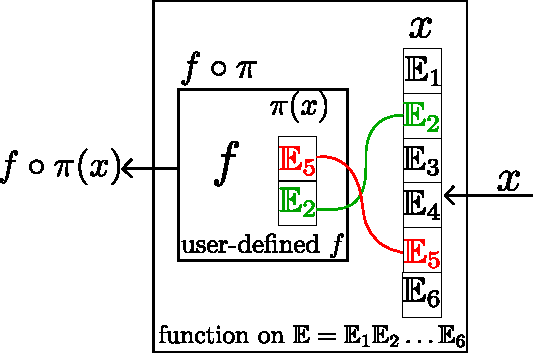
\includegraphics[width=.5\linewidth]{auto_mapping_text.pdf}
\caption{automatic variable mapping}
\label{fig:auto_map}
\end{figure}

%%%%%%%%%%%%%%%%%%%%%%%%%%%%%%%%%%%%%%%%%%%%%%%%%%%%%%%%%%%%%%%%%%%%%%%
%                        PROBLEM FORMULATION                          %
%%%%%%%%%%%%%%%%%%%%%%%%%%%%%%%%%%%%%%%%%%%%%%%%%%%%%%%%%%%%%%%%%%%%%%%

\section{Problem formulations}
\label{sec:problem_formulations}

Let $q=[q_F^T; q_r^T]\in SE(3)\times \mathcal{M}_r$ be the combination of the free-flyer of the robot $q_F\in SE(3) = \mathbb{R}^3 \times SO(3)$ and the articular parameters $q_r\in\mathcal{M}_r$.
Let $\mathcal{W}_i(p)=\{f_i,m_i(p)\}$ be the wrench (force+moment) applied by the environment onto the robot at contact $i$ and expressed on point $p$.
A frame $F$ is composed of a reference point and an orthonormal basis of 3 vectors $F = \{O, (\vec{x}, \vec{y}, \vec{z})\}$.
For frames define on a surface, with one vector of $(\vec{x}, \vec{y}, \vec{z})$ being the outbound normal to the surface, and the two others tangent, we rename $\vec{n}$ the normal one and $\vec{t}, \vec{b}$(tangent and bitangent) the two other ones, ensuring that $(\vec{n}, \vec{t}, \vec{b})$ is an orthonormal direct basis.
When a frame is denoted with the subscript i, $F_i$, all its components are added the same subscript.

Here is a list of constraints that we consider in our problems:

\begin{itemize}
\item Joint limits ${q^-} \leq q_r \leq {q^+}$:\\
These cannot be directly translated on manifolds other than $\mathbb{R}^n$.
For example, spherical joints can be parametrized on $S^2 \times \mathbb{R}$, then the $S^2$ part can be limited by a cone, and the $\mathbb{R}$ part can have real bounds(in that case the limit constraint is not a simple bound constraint, but writes as $f(q_r)\leq 0$).

%\item The contact constraint consists in identifying the features of two frames $F_1$ and $F_2$.
%For example, for a planar contact, we can write the constraints~\Eqref{eq:planar_contact_bad}.
%\begin{equation}
  %\left\{
  %\begin{array}{ll}
    %\overrightarrow{O_1O_2}\cdot\vec{n_1} = 0\\
    %\vec{n_2} = -\vec{n_1} \\
  %\end{array}
  %\right.
%\label{eq:planar_contact_bad}
%\end{equation}
%In practice, for a better numerical behavior of the optimization, we write that $\vec{n_2}$ is perpendicular to the plan $\{O_1, \vec{t_1}, \vec{b_1}\}$ and has opposite direction with $\vec{n_1}$,~\Eqref{eq:planar_contact}:
%\begin{equation}
  %\left\{
  %\begin{array}{ll}
    %\overrightarrow{O_1O_2}\cdot\vec{n_1} = 0\\
    %\vec{n_2}\cdot\vec{n_1} \leq 0 \\
    %\vec{n_2}\cdot\vec{t_1} = 0 \\
    %\vec{n_2}\cdot\vec{b_1} = 0
  %\end{array}
  %\right.
%\label{eq:planar_contact}
%\end{equation}
%Note that on $F_2$ only the point $O_2$ and the vector $\vec{n_2}$ are necessary.
%Other types of contacts can be created that way, by equalizing other features, as explained in~\cite{escande:ras:2013}.
%For example, we can fix the contact to a given position and orientation by adding to it the following set of equation~\Eqref{eq:fix_planar_contact} that locks the degrees of freedom of rotation around the normal and translation in the tangent plane of the contact:
%\begin{align}
  %\left\{
  %\begin{array}{ll}
    %\overrightarrow{O_1O_2} \cdot \vec{t_1} = 0 \\
    %\overrightarrow{O_1O_2} \cdot \vec{b_1} = 0 \\
    %\vec{b_2} \cdot \vec{t_1} = 0 \\
    %\vec{t_2} \cdot \vec{b_1} = 0 \\
    %\vec{t_2} \cdot \vec{t_1} \leq 0
  %\end{array}
  %\right.
%\label{eq:fix_planar_contact}
%\end{align}
%Those two sets of equations~\Eqref{eq:planar_contact} and~\Eqref{eq:fix_planar_contact} can easily be recombined to generate other types of constraints (e.g.\ fixing only the translation, or only the rotations\ldots).

\item The Frame constraint is a generic type of constraint that consists in blocking a predefined set of degrees of freedom of one frame $F_2$ w.r.t. another frame $F_1$.
By default, the frame $F_2$ has 6 degrees of freedom w.r.t. $F_1$, three translational degrees of freedom TX, TY, and TZ, respectively along $\vec{x_1}$, $\vec{y_1}$ and $\vec{z_1}$ and three rotational ones RX, RY, and RZ, respectively around $(O_1,\vec{x_1})$, $(O_1,\vec{y_1})$ and $(O_1,\vec{z_1})$.
We can write constraints such that any combination of the translational degrees of freedom is blocked:

\begin{align}
  \text{If TX is blocked: } \overrightarrow{O_1 O_2} \cdot \vec{x_1} = 0 \\
  \text{If TY is blocked: } \overrightarrow{O_1 O_2} \cdot \vec{y_1} = 0 \\
  \text{If TZ is blocked: } \overrightarrow{O_1 O_2} \cdot \vec{z_1} = 0
\end{align}

Similarly, any pair of rotational degrees or the three of them can be blocked (blocking only one rotation is not possible with that formalism).
If the three rotations RX, RY, RZ are blocked, we get the set of constraints~\ref{eq:3_rotations_blocked}:
\begin{equation}
\label{eq:3_rotations_blocked}
\begin{cases}
  \vec{z1}\cdot\vec{y2} = 0 \\
  \vec{z1}\cdot\vec{x2} = 0 \\
  \vec{x1}\cdot\vec{y2} = 0 \\
  \vec{z1}\cdot\vec{z2} \geq 0 \\
  \vec{y1}\cdot\vec{y2} \geq 0
\end{cases}
\end{equation}

When two rotational degrees of freedom are blocked, we get the set of constraints~\ref{eq:2_rotations_blocked}
To generalize the following formulas, we rename the axis X, Y, and Z with respect to their respective roles in this constraint.
The one rotational degree that remains free is denoted N with vector $\vec{n}$, and the two others are denoted T and B, with vectors $\vec{t}$, and $\vec{b}$.
Those 3 vectors are ordered such that $(\vec{n}, \vec{t}, \vec{b})$ is an orthonormal direct basis.

\begin{equation}
\label{eq:2_rotations_blocked}
\begin{cases}
  \vec{n_2}\cdot\vec{n_1} \geq 0 \\
  \vec{n_2}\cdot\vec{t_1} = 0 \\
  \vec{n_2}\cdot\vec{b_1} = 0
\end{cases}
\end{equation}

In theory, one could simply write that constraint as $\vec{n_1}=\vec{n_2}$, but in practice, this formulation leads to bad numerical behavior of the optimization, thus we prefer~\ref{eq:2_rotations_blocked}.

All those independent sets of constraints can be combined to create a wide variety of geometric constraints.
For example, one can create a mobile planar contact constraint with normal $\vec{z}_1$ by blocking TZ, RX and RY.
A punctual contact constraint can be devised by blocking TX, TY and TZ.
To completely fix the position of $F_2$ w.r.t. $F_1$, one can block TX, TY, TZ, RX, RY, and RZ.
And many other types of custom constraints can be devised with this formulation.

In the event that the two frames do not have a satisfying configuration to write the desired constraint with this formalism (for example, if one wants to write a planar contact between two surfaces $S_1$ and $S_2$, where $\vec{z_1}$ and $\vec{z_2}$ are outbound normal vectors, then equation~\ref{eq:2_rotations_blocked} is not satisfactory because we want to oppose $\vec{z_1}$ and $\vec{z_2}$, not identify them.), then user is required to define a new frame $F_2'$ that is a constant 3D transformation away from $F_2$ (in that case a rotation of $\pi$ around $(O_1,\vec{x_1})$ would suffice).

\item The stability constraint ensures that the Euler-Newton equation~\Eqref{eq:NewtonWrench} is balanced for the set of external wrenches applied to the robot (gravity $\mathcal{W}_G$ and contact forces $\mathcal{W}_i$).
\begin{equation}
  \sum_{i}{\mathcal{W}_i(p)} + {\mathcal{W}_G(p)} = 0
  \label{eq:NewtonWrench}
\end{equation}
For each contact that bears forces (`stability' contact), a wrench applied on the robot at the contact point is added to the problem.
If the contact is added through a frame constraint between $F_1$ and $F_2$, the wrench can be formed by a combination of elementary components that are:
\begin{itemize}
\item FX: force along $\vec{x_1}$, value $f_x$
\item FY: force along $\vec{y_1}$, value $f_y$
\item FZ: force along $\vec{z_1}$, value $f_z$
\item MX: moment around $(O_1,\vec{x_1})$, value $m_x$
\item MY: moment around $(O_1,\vec{y_1})$, value $m_y$
\item MZ: moment around $(O_1,\vec{z_1})$, value $m_z$
\end{itemize}
That wrench is parametrized on a $\mathbb{R}^m$ with $m$ the number of components used.
%For punctual contacts, the moment part is null on the application point.
%Only a parametrization of the force part on $\mathbb{R}^3$ is needed.
We model the resultant wrench of planar contacts as a combination of punctual forces applied at each vertex of the contact polygon.
In the case of interaction forces between 2 robots, only one wrench is created and it is used as is in the stability equation of one robot and its opposite is used for the stability of the second robot.
That way, we are guaranteed that the forces in between the robots are balanced and we can evaluate the stability of each robot separately.

\item The friction cone constraint can be used to limit the tangential part of any force to avoid slippage.
We write it as~\Eqref{eq:friction} (with $\mu$ the friction coefficient)
\begin{equation}
  \begin{split}
    \mu^2f_z^2-f_x^2-f_y^2 \geq 0 \\
    f_z \geq 0
  \end{split}
  \label{eq:friction}
\end{equation}

\item The rotational friction limit constraint can be used to limit the friction torque of any force to avoid slippage.
We write it as~\Eqref{eq:frictionTorque} (with $\sigma$ the rotational friction coefficient)
\begin{equation}
  \begin{split}
    \sigma^2f_z^2-m_z^2 \geq 0 \\
    f_z \geq 0
  \end{split}
  \label{eq:frictionTorque}
\end{equation}


\item The collision avoidance constraint can be defined between any two bodies.
A convex mesh is attached to each body involved in the constraint.
We denote them $C_1$ and $C_2$.
We use the {\tt sch-core} library described in~\cite{benallegue:icra:2009} that implements an efficient GJK algorithm to compute the distance $d(C_1,C_2)$ between 2 convex shapes and its derivative.
A description of strictly convex hulls that can be used for this purpose is detailed in~\cite{escande:itro:2014}.
For each collision avoidance constraint, we require that the distance between the two convex remains superior to a minimal distance $d_{\min}$
\begin{equation}
  d(C_1, C_2)\geq d_{\min}
\end{equation}

\item The torque limit constraint makes use of the Inverse Statics algorithm~\ref{alg:ISmatrix} to compute the torques in all the joints of every robots and their derivatives are computed by algorithm~\ref{alg:TJC}.
Denoting $\tau_i$ the torque in joint $i$ resulting from the robot's configuration and the external forces applied on it, and its lower and upper limits as $\tau_i^-$ and $\tau_i^+$. The torque limit constraint writes as follows:
\begin{equation}
  \forall i,\ \tau_i^- \leq \tau_i \leq \tau_i^+
\end{equation}
\end{itemize}


%The frame in which the constraints are written matters critically.
Most often, the frame's configuration depends on a part of the optimization variables, that must be accounted for in computing the constraints' Jacobian.
Our framework computes such dependencies automatically.

Another important part is the problem's cost function.
Any function of the problem's variables that returns a scalar value can be used as a cost function.
In our formulation, we take a sum of cost functions into account, several different functions $f_i$ over different variables can be defined separately.
And then combined in a weighted sum as the problem's cost function (with $w_i$ the weight of function $f_i$):
\begin{equation}
  cost = \sum\limits_i w_i f_i
\end{equation}
Taking advantage of our framework, the set of variables over which the cost function is defined, its value and its derivatives are then computed automatically.

A typical cost function is the distance to a reference posture $q_0$.
On a robot that has all its articulations parametrized on $\mathbb{R}$ the distance can be expressed simply with the Euclidean norm $d = \norm{q_r-q_0}^2$.
Since we work on non-Euclidean manifolds, the logarithm function on the manifold must be used.
It gives the distance vector between two points in the tangent space, the norm of this vector can be used as a distance.
So we get $d = \norm{\text{log}_{q_0}(q_r)}^2$ (note that on $\mathbb{R}^n$, $\norm{\text{log}_{q_0}(q_r)}^2 = \norm{q_r - q_0}^2$)

We can also use the cost function to set a target value $v$ for the value of a contact force $\vec{F}$ in a given direction $d$. By simply implementing the following function:
\begin{equation}
  f = \norm{\vec{F}\cdot\vec{d}-v}
\end{equation}

The list of constraints and cost functions that can be used in robotics posture generation problems can be extended, and this process is made easier by our framework.


%%%%%%%%%%%%%%%%%%%%%%%%%%%%%%%%%%%%%%%%%%%%%%%%%%%%%%%%%%%%%%%%%%%%%%%
%                           IMPLEMENTATION                            %
%%%%%%%%%%%%%%%%%%%%%%%%%%%%%%%%%%%%%%%%%%%%%%%%%%%%%%%%%%%%%%%%%%%%%%%

\section{Implementation}
\label{sec:implementation}

In this section, we provide an overview of some of the key elements of the framework:

\paragraph{Problem's configuration:}
The implementation of the core structure of a posture generation problem is written in \texttt{C++}.
A text file in YAML format can be used to configures the solver and some custom parameters of the problem; It is parsed at runtime to avoid having to recompile the problem for every configuration change.
Also, some \texttt{Python} bindings have been developed to allow writing the core structure of the problem without compilation.
%We use two types of configuration files:
%\begin{itemize}
  %\item A default configuration file contains all the usual data, like the paths to robots description directories, as well as some data about each robot, like the lists of usual self-collisions used per robot, etc\ldots\\ {\tt problem-generator/configs/problemGeneratorConfig.yml.in}
  %\item A problem specific configuration file that contains all the data necessary to describe the problem, like the list of robots, the location of some geometric features, some solver parameters, the choice for a robot to have a fixed basis, or torque limits and anything else that can help specify the problem.
%\end{itemize}

\paragraph{The Robot class:}
%It is instantiated from a Robot::Init structure that contains all the necessary data for its construction.
%Which includes its name, its URDF path, the path of its collision meshes, some booleans defining if the robot is fixed, has torque limits, etc\ldots
%On instantiation of a robot, we use this URDF to instantiate the RBDyn objects that are used to compute the Forward Kinematics and Inverse Statics of the robot: a MultiBody, a MultiBodyGraph and a MultiBodyConfig, as well as its joint, torque limits, and the manifold in which the variables of the robot live.
%The robot object is equipped with an external\_forces object that handles the external forces applied to it, and a torques object that handles its joint torques.
%A Frame is created on each of the bodies of the robot.
%A set of predefined surfaces on bodies can be loaded from an rsdf file.
%A set of collision convex meshes attached to the bodies of the robot is created based on a provided list of mesh files.
%The configuration of a robot depends on its articular parameters, to hanble that, the robot object contains an update method that runs the Forward Kinematics algorithm and updates the transformations of each body and its jacobian, which, by extension updates the its body frames. Every body frames get their transformation's values and derivatives from those quantities.
The RBDyn library contains all the low-level tools and algorithm to compute the kinematics and statics of a robot.
The robot class is built on top of RBDyn to provide high-level functionalities while adapting it to our manifold formalism (which RBDyn does not handle natively).
The basic structure of the robot is extracted from its URDF description file.
The main functionality of the robot class is to create a Frame attached to each of its bodies and to update their transformations and derivatives based on the robots articular variables.
It also maintains the transformations of all the collision meshes and contains the joint and torque limits, as well as the manifold on which its variables live.
Additionally, it contains some useful objects used to maintain and update the external forces applied on the robot, as well as the joint torques.

\paragraph{The Function Class:}
The functions that we use derives from the Roboptim's functions.
As such, they are able to compute their return value and derivative for a given input.
Functions can conveniently be defined through our expression framework to take advantage of their automatic derivation.

\paragraph{The Constraint class:}
A constraint object contains all the necessary elements for the description of a mathematical constraint.
That is, a function $h$ and the manifold $\mathcal{M}_c$ on which it should be applied, as well as its lower bound $l$, upper bound $u$ and the scaling factor of the constraint.
Once a constraint is instantiated by the problem, the input mapping $\pi$ from the problem's complete manifold $\mathcal{M}$ to the function's application manifold is computed.
The constraint that will then be used in the optimization for a given iterate $x$ can be written as:
\begin{equation}
  l \leq h\circ\pi(x) \leq u
\end{equation}
%A constraint is a function accompanied by its application manifold, bounds and scaling factors.
%It is convenient to use a function built by our expression framework here, to take advantage of their automatic derivation and variables.
%Every constraint has a geometric part and a stability part that are added separately to the problem.
Constraints can be equipped with an `addStabilityToProblem' method that is used to specify the forces generated by the constraint to add to the stability constraint of the problem.
%The stability part is mainly used to add contact forces to the stability constraint.

\paragraph{The Frame Constraint class:}
It describes a very useful type of constraint between two frames $F_1$ and $F_2$.
It implements the Frame constraint that we described in Section~\ref{sec:problem_formulations} with some additional features.
This specific constraint is composed of four distinct parts:
\begin{itemize}
  \item The geometric constraint generates the constraints associated with the user's choice of combination of degrees of freedom to block amongst TX, TY, TZ, RX, RY, RZ.
  \item The static constraint part (optional) instantiates the wrench to be added to the stability constraint of the problem based on the user's choice of components FX, FY, FZ, MX, MY, MZ.
  \item A custom geometric additional function field (optional) allows the user to add extra geometry constraints to the problem (through a \texttt{C++11} lambda that is executed after the geometric constraints are added to the problem).
  \item A custom static additional function field (optional) allows the user to add extra static constraints to the problem (through a \texttt{C++11} lambda that is executed after the constraint's wrench has been created and added to the problem).
\end{itemize}
The custom geometric additional function can typically be used to in the context of a planar contact to limit the position of $O_2$ to the inside of a polygon defined in the plan $(O_1,\vec{x_1},\vec{x_2})$.
As for the static additional function, it can be used to add constraints on the values of the constraint's wrench, for example, enforcing the friction cone constraints.

%In terms of geometry, the canonical constraints one can enforce between two frames consist in blocking each of the 6 degrees of freedom of $F_2$ w.r.t $F_1$, e.g.\ blocking the translation and rotations along each axis.
%We can combine any set of those canonical constraints to emulate any typical joint type between the two frames (fixed, planar, spherical, etc\ldots) and more.
%Any type of wrench can be composed the same way from the canonical wrenches (forces and moments along each axis).
%On top of those geometric and stability parts of that constraint, custom additional constraints can be added to it, for example requiring the origin of $F_2$, $O_2$, to be inside a polygon defined in $F_1$, or requiring that the forces generated by that constraint remain in their Coulomb friction cones.

\paragraph{The PostureProblem class:}
The PostureProblem class is in charge of building the complete optimization problem that represents our posture generation problem.
It creates and owns the robots present in the problem.
It registers all the variables and constraints of the problem as well as all the functions involved in the cost function.
Each function is likely to bring additional variables with it.
For each contact contributing to the balance, a variable representing the contact force is added to the problem.
The associated wrench is added to the stability constraints.
%Once the registration is complete, the complete manifold of the problem is generated and uses the information of the automatic mapping to `plug' each function with the correct sub-manifold.
Once the registration is complete, the complete manifold of the problem is generated and all the functions on manifold used in the problem will generate their input mapping that will project the complete variable of the problem onto the submanifold that the function is interested in.
Subsequently, the optimization problem can be generated and passed to the solver.
The communication between the solver and the generated problem is made through the RobOptim framework\footnote{\url{http://www.roboptim.net/}}~\cite{moulard:jsme:2013, moulard:jrsj:2014}.
After creating the complete manifold, the PostureProblem class can be used to facilitate the individual initialization of all the separate variables of the problem without the user having to worry about the indexes.
Finally, it can query the resolution of the problem by the solver and return the result.

\section{Examples of postures generation}
\label{sec:examples_of_postures_generation}

In this section, we present some scenarios solved with our posture generator and solver.
\paragraph{Application of a desired force}
In the context of using a robot to help humans in the construction of an aircraft, we formulate a problem where the HRP-4 robot is required to apply a desired force on a given point of the airplane's structure.
We denote $f_g$ the target value of the force in direction $\vec{d}$ and $\vec{f_c}$ the actual force at the contact point and the could simply implement the following function $f_{target}(f_c)$ to minimize to get the desired result:
\begin{equation}
  f_{target}(f_c) = {\left(\vec{f_c}\cdot\vec{d}-f_g\right)}^2
\end{equation}
In addition to that cost function, the robot needs to keep its foot on the ground, its left hand is used to lean on a beam of the structure to allow a longer reach with the right hand that is in contact with the wall.
Those constraints must be satisfied while respecting the joint and torque limits of the robot, maintaining balance and avoiding auto-collisions.
The result is depicted in figure~\ref{fig:comanoid}
\begin{figure}
  \centering
  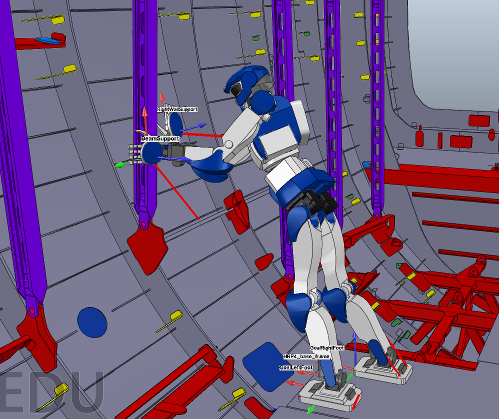
\includegraphics[width=0.6\linewidth]{comanoid.png}
  \caption{HRP-4 applying a desired force on a contact point with its right hand}
\label{fig:comanoid}
\end{figure}

\paragraph{Generating postures in highly constrained environment}
In this scenario, the HRP-4 robot is required to evolve in a highly constrained environment, in the sense that many obstacles limit its displacement, and it must avoid collision with them.
The goal is to real a panel of circuit breakers (in green on figure~\ref{fig:getafe}) to activate them.
We generated a sequence of steps to reach that panel and then some postures to reach different points of this panel.
In figure~\ref{fig:getafe}, we show some extracts of this sequence of postures.
In each of them the two foot are in planar contact with the ground, alternatively bearing forces, while always respecting the joint, torque limits, collision avoidance, and stability constraints.
On the last posture, the top left corner of the panel is reached with the tip of the right hand of the robot.
\begin{figure}
  \centering
  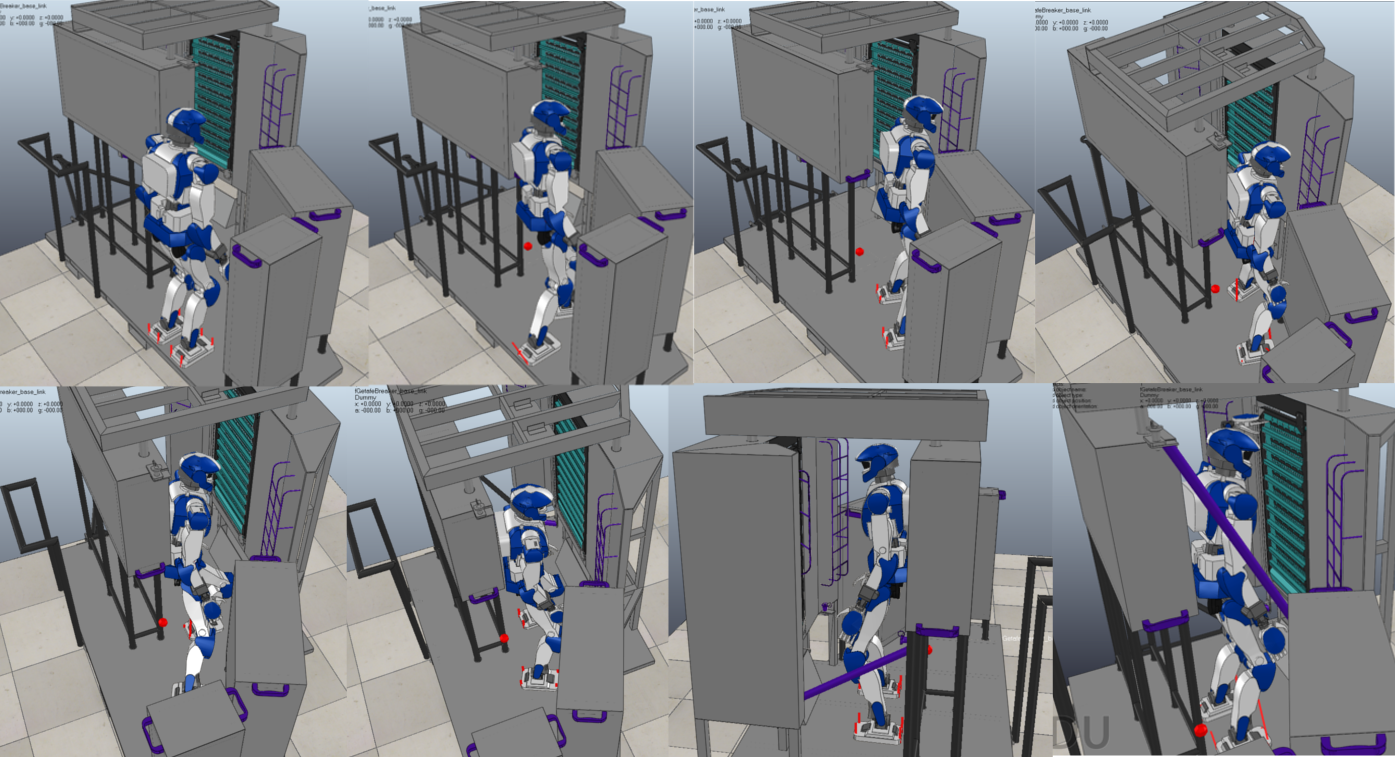
\includegraphics[width=\linewidth]{getafeSequence.png}
  \caption{Extracts of a sequence of postures with HRP-4 entering a constrained environments to reach a point on a panel of circuit breakers (in green)}
\label{fig:getafe}
\end{figure}

%%%%%%%%%%%%%%%%%%%%%%%%%%%%%%%%%%%%%%%%%%%%%%%%%%%%%%%%%%%%%%%%%%%%%%%
%                     CONTACT ON NON-FLAT SURFACE                     %
%%%%%%%%%%%%%%%%%%%%%%%%%%%%%%%%%%%%%%%%%%%%%%%%%%%%%%%%%%%%%%%%%%%%%%%

\section{Contact on non-flat surfaces}
\label{sec:contact_on_non_flat_surfaces}

Writing relations between geometric quantities defined in frames allows to describe a large variety of contacts.
%It is especially convenient when the contact points are predefined or when the geometric relations are simple to express, like for the inclusion of 2 convex polygons in each other in the context of a planar contact.
In particular, it allows to write most types on geometric constraints between canonical geometric shapes (point, line, plane).
The most common type of contact constraint encountered is the contact between two surfaces $S_1$ and $S_2$.
The set of equations used to define that type of constraint can be obtained through a frame constraint blocking TZ, RX and RY. Provided that the correct frames are defined, $F_1$ on $S_1$ with $\vec{z_1}$ normal outbound and $F_2$ on $S_2$ with $\vec{z_2}$ normal inbound, the constraint writes as:

\begin{equation}
  \left\{
  \begin{array}{ll}
    \overrightarrow{O_1O_2}\cdot\vec{z_1} = 0\\
    \vec{z_2}\cdot\vec{z_1} \geq 0 \\
    \vec{z_2}\cdot\vec{x_1} = 0 \\
    \vec{z_2}\cdot\vec{y_1} = 0
  \end{array}
  \right.
\label{eq:planar_contact}
\end{equation}

When the two surfaces are flat, a contact between them can be written simply with the set of equations~\Eqref{eq:planar_contact}.
In that case, the quantities involved in the constraint are invariant with the location of the contact point, thus, the equations are valid for any point of the surface (in particular, the normal vector is the same for any point on the surface).
%When it comes to non-flat surfaces, the orientation of the normal vector changes with the location of the contact point, if the contact point is fixed and predefined, the set of equation~\Eqref{eq:planar_contact} can describe the constraint, otherwise, it is not sufficient.
When it comes to non-flat surfaces, the location of the frames used in equations~\Eqref{eq:planar_contact} matters, as the quantities in the constraint equations depend on it.
%(in particular, the normal vector can vary for any point on the surface).

%We propose to describe that type of contact by parametrizing the contact surface, and using an additional variable on which the location of the contact point and its normal vector are parametrized.
%We remind that a contact constraint between $F_1$ and $F_2$ described by eq~\Eqref{eq:planar_contact} requires the full $F_1$ frame and on $F_2$, only the origin and its normal vector are necessary.

%If any(either or both) of the two surfaces in contact is non-plane, finding the exact location of the contact point on the surface is necessary, because then, the normal to the contact is not known in advance.

We propose to add an additional variable $u_S$ to our optimization problem to represent the location of the contact frame on a non-flat surface.
This gives the ability to our solver to choose the optimal contact position on a non-flat surface.
Depending on its shape, the manifold $\mathcal{M}_S$ on which the surface is parameterized can be $\mathbb{R}$, $\mathbb{R}^2$ or $S^2$.
Then we can write the contact constraint on that parametrized frame with ease.
\begin{equation}
\label{eq:param_frame}
  \mathcal{F}(u_S\in \mathcal{M}_S) = \{O(u_S), (x(u_S), y(u_S), z(u_S))\}
\end{equation}
In this section, we will successively present several ways to parameterize various non-flat surfaces to generate contacts with them.

%We propose to handle that case by paramaterizing the contact frame on the surface with a variable $u_S$ on a 1 or 2-dimensional manifold $\mathcal{M}_S$ (which, depending on the shape, could be $\mathbb{R}$, $\mathbb{R}^2$ or $S^2$), and adding this variable to our optimization problem.
%Then we can write the contact constraint on that parametrized frame with ease.
%\begin{equation}
%\label{eq:param_frame}
  %\mathcal{F}(u_S\in \mathcal{M}_S) = \{O(u_S), (x(u_S), y(u_S), z(u_S))\}
%\end{equation}

%In that case, an additional set of variables $u_S\in \mathcal{M}_S$ is added the optimization problem and we can desctibe  as well as the constraint set \Eqref{eq:planar_contact} depending on it.

\subsection{Application to plan-sphere contact}
We consider the contact between a body's flat surface $S_B$ of normal $n_B$, with the surface of a sphere $S_s$ of center $c_s$, radius $r_s$, and let $p_s$ and $n_s$ be a point and its normal on $S_s$.
The most general way to express such a constraint is to ensure that $p_s$ is on $S_B$ and that $n_s$ and $n_B$ are opposite.
To do that, we create a variable $v_{S^2}$ on $S^2$, add it to our optimization problem and map $p_S$ and $n_S$ on it.
In our framework, this constraint is expressed exactly as the contact between 2 planar surfaces, once the mappings of $p_s(v_{S^2})$ and $n_s(v_{S^2})$ are done.
In a framework that does not handle manifolds, it would require to setup a specific constraint, ensuring that the distance between $c_s$ and $S_B$ is equal to $r_S$.

In Fig.~\ref{fig:contact_plan_sphere} we show the results obtained by solving a problem where the HRP2-Kai robot has to keep its feet in contact with the ground at fixed positions, touch a sphere with a side of its right wrist and point as far as possible in a given direction $d$ with its left hand, under balance constraints.
The top row of Fig.~\ref{fig:contact_plan_sphere} shows the results for this problem with several different $d$.
%It shows that our optimization algorithm finds an optimal contact point on the sphere to reach its goal as best as possible while satisfying the given constraints.
In every situation, the projection of the CoM is outside the polygon of support, meaning that such postures would not be reached without leaning on the sphere.

\begin{figure}
\centering
  \centering
  \setlength\fboxsep{0pt}
  \setlength\fboxrule{1pt}
  \fbox{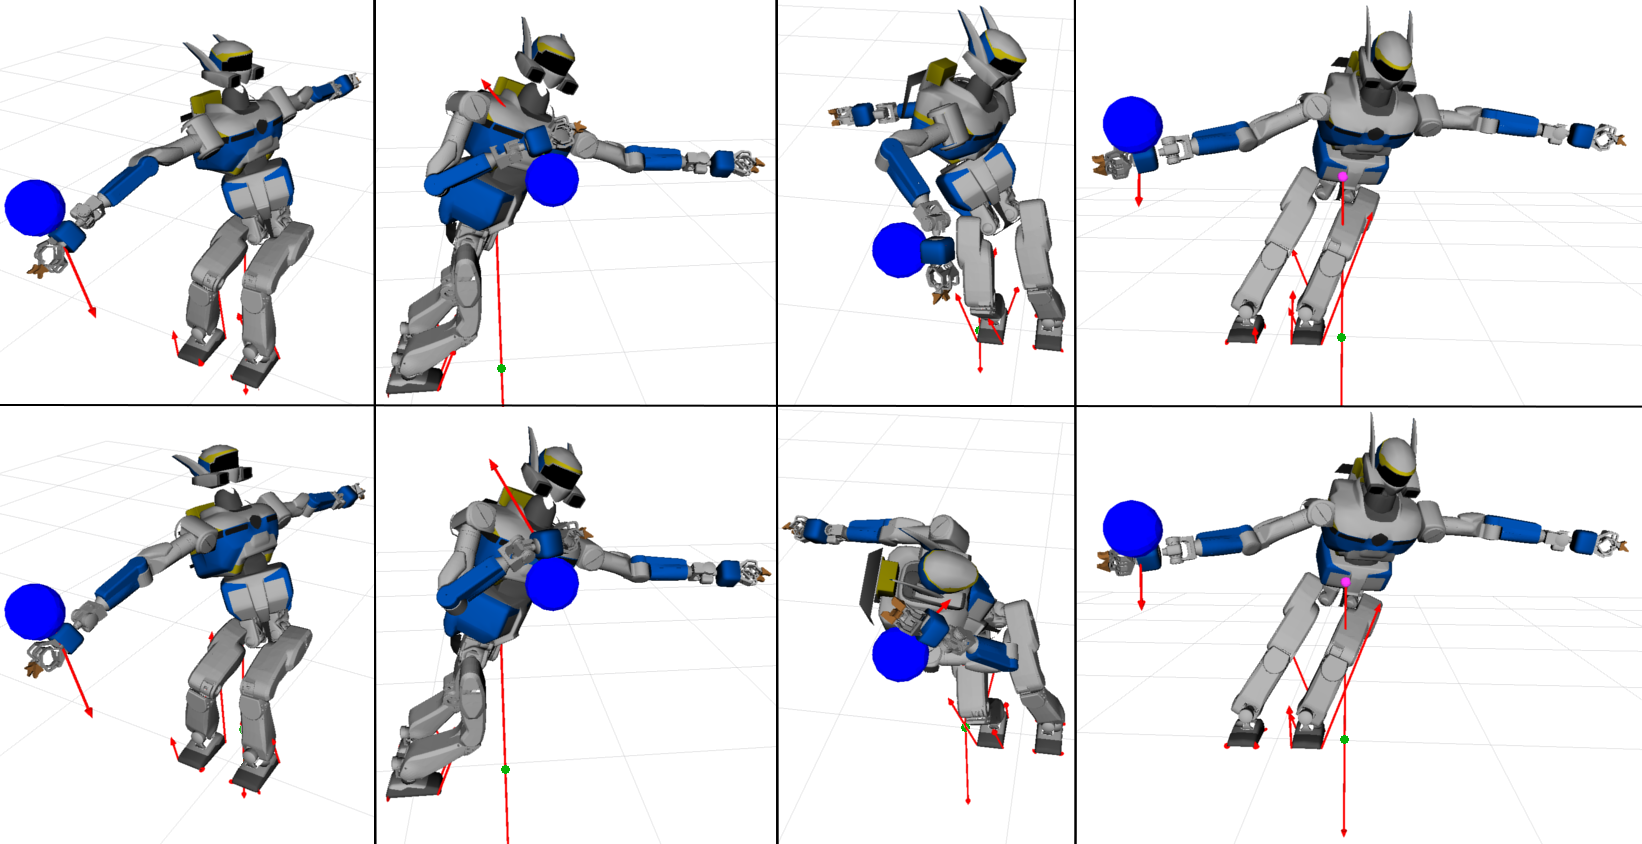
\includegraphics[width=.95\textwidth]{4directionsStrokesWithCoM.png}}
  %\fbox{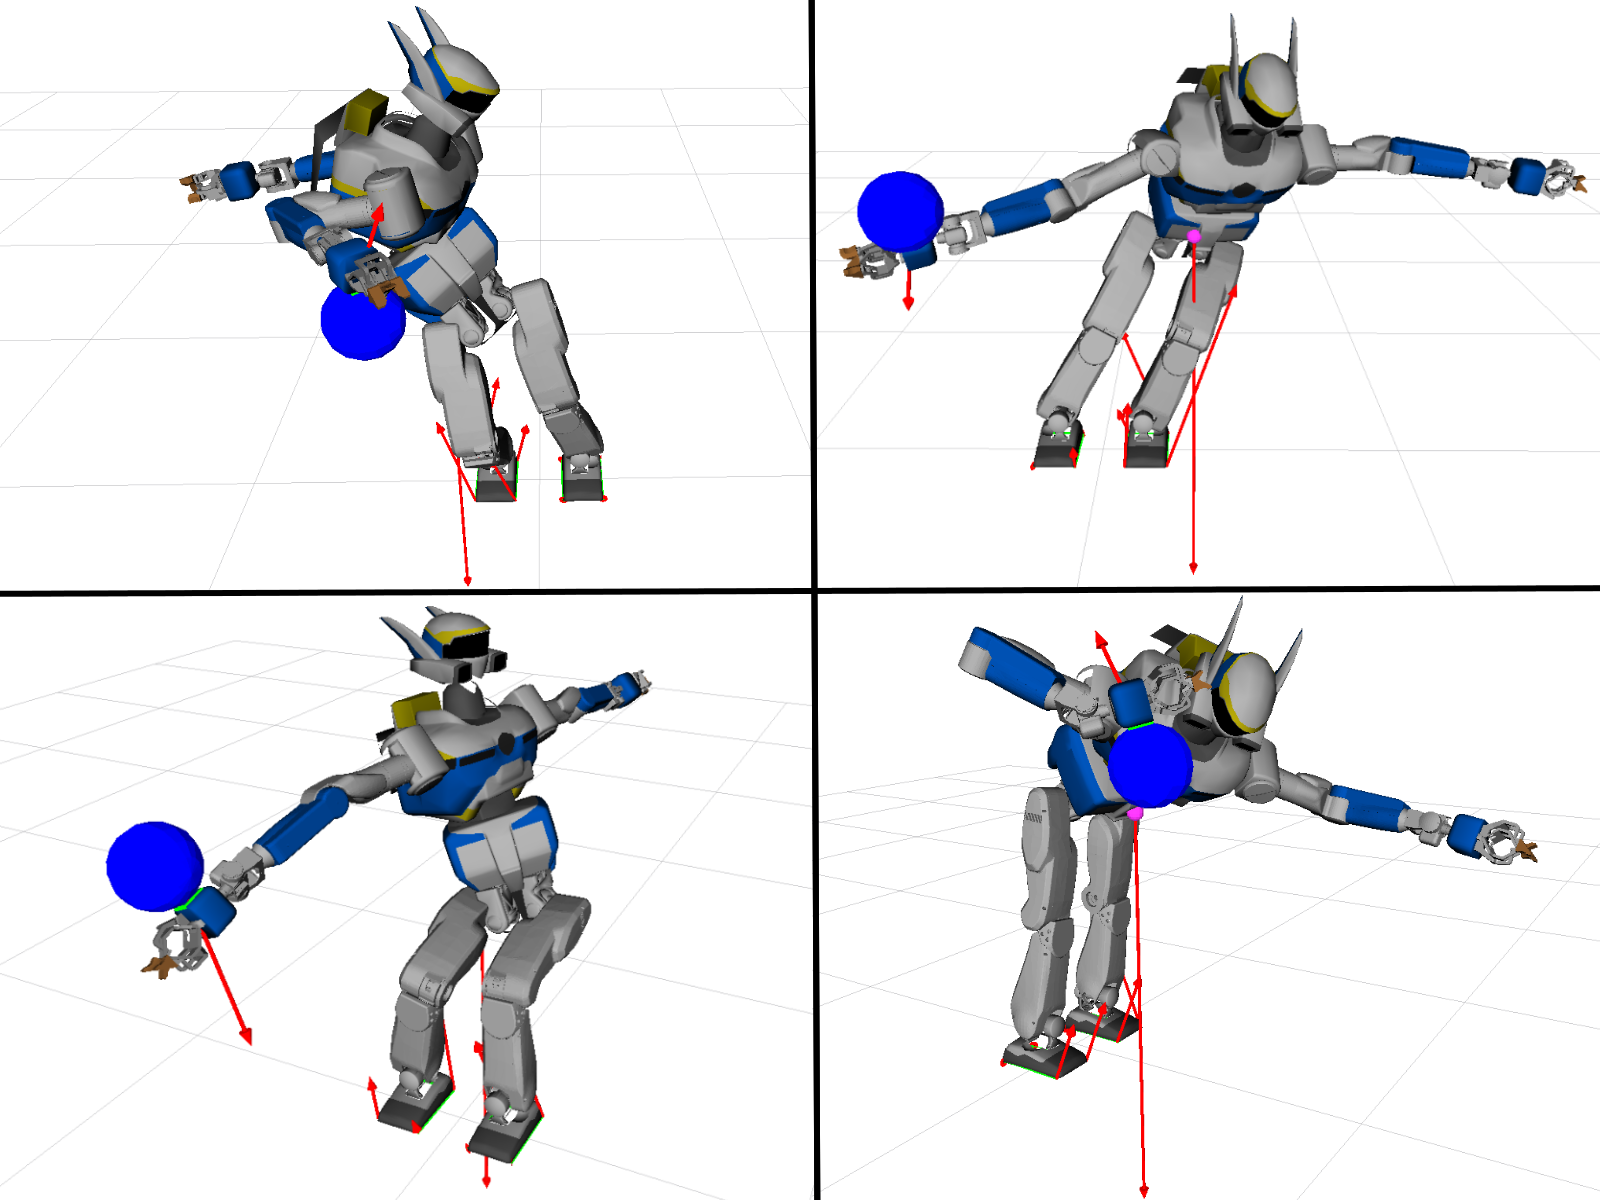
\includegraphics[width=.95\linewidth]{papers/Humanoids2015/figure/contact_plan_sphere_4_directions.png}}}
  \caption{HRP2-Kai leaning on a sphere with its right wrist to point its left gripper as far as possible in 4 cardinal directions.
  Top row: semi-predefined contact; Bottom row: free contact with parametrized wrist.
  Projection of the CoM on the ground (green dots)}
\label{fig:contact_plan_sphere}
\end{figure}

\subsection{Contact with parametrized wrist}

\begin{figure}[!htb]
\centering
  \centering
  \setlength\fboxsep{0pt}
  \setlength\fboxrule{1pt}
  \fbox{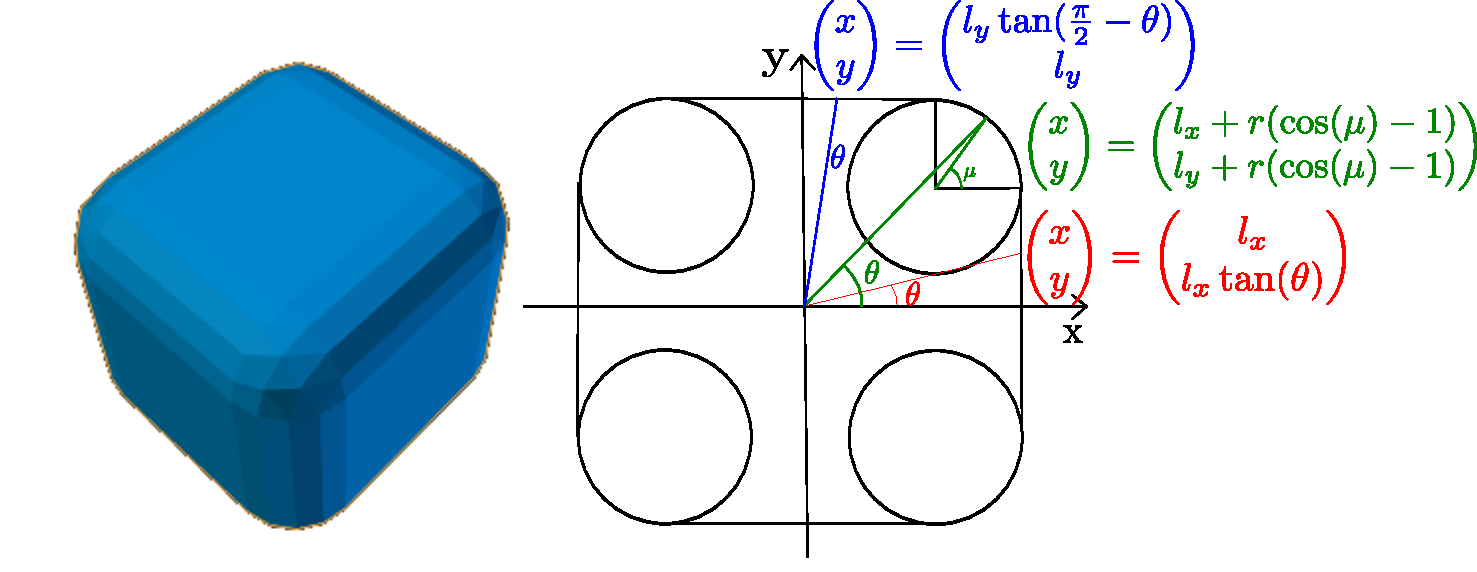
\includegraphics[width=.65\linewidth]{param_wrist_detail.pdf}}
  %\fbox{\includegraphics[width=.95\linewidth]{papers/Humanoids2015/figure/param_wrist_detail.png}}
\caption{Parametrization of the wrist of HRP2-Kai}
\label{fig:param_wrist_detail}
\end{figure}

Being able to choose the location of the contact point on the sphere is interesting, but a limitation of this formulation is that the contact point on the wrist of the robot is restricted to one single user-defined face.
Instead, we describe the shape of the wrist body as a parametric function and let the contact point on the wrist as well as its counterpart on the sphere, result from the optimization process.
The section of HRP2-Kai's wrist is a square with rounded edges.
We parametrize this shape as shown in Fig.~\ref{fig:param_wrist_detail}:
we consider the angular coordinate $\theta$ of the point on the section.
It is added as a variable on $\mathbb{R}$ to the problem.
The shape of the quarter of section $[0;\pi/2]$ is a succession of a vertical line, a quarter of a circle and a horizontal line.
This pattern is repeated for the 3 other quarters.
The equations are given in Fig.~\ref{fig:param_wrist_detail}.
In our framework, we define the function describing the shape of the wrist, create a frame parametrized by that function and then define the contact between that frame and the point and normal on the sphere.
This formulation not only is very easy to implement but most importantly, allows for richer posture generations.
The optimization algorithm chooses the contact point on the sphere as well as the contact point on the wrist, which leads to a wider accessibility range, and a better satisfaction of the cost function.

The bottom row of Fig.~\ref{fig:contact_plan_sphere} displays the results of this simulation for the robot pointing in 4 directions.
Notice that on the 2nd and the 4th (pointing forward and to the left) images, the results for the 2 types of models are nearly identical, whereas in the 1st and 3rd images, different faces of the wrist have been chosen (On the 1st, the wrist is rotated by $180^{\circ}$, and $90^{\circ}$ on the 3rd).
In these 4 cases, the contact with parametrized wrist gives a better value of the objective function (the left hand points further).
This observation scales:
we solved this problem for 5000 random pointing directions, and in average, the contact with parametrized wrist allows to reach 5mm further.
The success rate of the solver is $98.5\%$ in the parametrized wrist case against $99.9\%$ when the face is fixed.
The numbers of iterations are similar.

%Also, that kind of formulation makes it easier for the user to generate satisfactory postures, as he does not need to specify the plan contact surface anymore.
This method is certainly scalable, and can be used for any kind of humanoid robot and environment.
Yet, it requires having a parametric equation of the surface.

\subsection{Contact with an object parametrized on the unit sphere}

In this case, we want the HRP-4 robot to carry a cube with its two hands.
The most general way to do it is to select a face of the cube for each contact and to enforce the contact between that face and the hand's surface.
We propose to approximate the cube with a superellipsoid and to parametrize the resulting shape on $S^2$, thus adding a variable on $S^2$ to our problem.
The implicit equation of a superellipsoid is $S(x,y,z) = 0$, with
\begin{equation}
  S(x,y,z) = {\left( \left|\frac{x}{A}\right|^r + \left|\frac{y}{B}\right|^r\right)}^\frac{t}{r} + \left|\frac{z}{C}\right|^t - 1
  \label{eq:super_ellipsoid}
\end{equation}

A point in $S^2$ is represented by a vector $v=(x,y,z)$ in $\mathbb{E} = \mathbb{R}^3$.
To a given unit vector $v$ we associate a point $\alpha v$ on the surface of the superellipsoid by solving $S(\alpha v) = 0$ for $\alpha$.
At this point, the normal is given by $\dfrac{\nabla S(\alpha v)}{\left\|\nabla S(\alpha v)\right\|}$ which simplifies into $\dfrac{\nabla S(v)}{\left\|\nabla S(v)\right\|}$.
%It returns the intersection between any unit vector and the surface of the super ellipsoid.
%Also we generate a similar function that returns the normal of the intersection point.
Given this parametrization, we write a contact constraint between the frame of the hand of the robot and the point and normal on the surface of the superellipsoid.

In Fig.~\ref{fig:hrp4_cube} we present some results for a posture generation problem with manipulation: On the left side, the feet are free to move on a sphere, and, on the right side, the left foot position is fixed and the right foot is free to move on the ground.
The hands must be in contact with the cube.
The cube is free to move (parametrized by $\mathbb{R}^3 \times SO(3)$) and has it own set of Euler-Newton equations, which must be fulfilled.
%On the accompanying video, one can observe how the contact points on the cube evolve along with the optimization.
%For each contact with the cube, a variable on $S^2$ is added to the problem to parametrize the contact point.
%Each hand is in contact with a point and normal on the cube.

\begin{figure}
\centering
  \centering
  \setlength\fboxsep{0pt}
  \setlength\fboxrule{1pt}
  \fbox{\includegraphics[width=.8\linewidth]{hrp4CubeOnSphere.png}}
\caption{HRP4 carrying a 2 kg cube.
Left: the objective function is to maintain the cube at a given position.
Right: it is to put the cube as far as possible in a given direction}
\label{fig:hrp4_cube}
\end{figure}

\section{Contact with Complex Surfaces}
\label{sec:contact_with_complex_surfaces}

We have presented some methods to formulate contact constraints with parameterized surfaces.
The surfaces that we used so far could all be approximately represented by closed-form equations (sphere, superellipsoid, wrist of HRP-2).
%We showed that to generate contacts between a body of a robot and simple geometric surfaces (sphere, superellipsoid, wrist of HRP2) we can devise some ad hoc parametrization of the surface and write constraints on the resulting approximated surface.
This is sufficient to tackle a large number of interesting scenarios, especially for robots in structured environment~\cite{vaillant:humanoids:2014} \cite{vaillant:autonomousrobots:2016}.
However, contacts with more complex objects are needed too, for unstructured environment or for manipulating objects.

To work with derivative-based optimization algorithms, such as SQP or Interior Points, the functions involved in the optimization problem need to be at least $C^1$ and gradients must be full rank at the solution (for ensuring constraints qualification, see~\cite{nocedal:book:2006}).
Since the contact point can be anywhere on our parametrized surface, the gradients must be full rank everywhere.

In the previously presented parametrizations of typical geometric shapes (sphere, superellipsoid\ldots) those continuity requirements are not a problem.
But for a given object, a parametrization of its surface is rarely available, especially a parametrization conforming with the continuity requirements.
On the contrary, we usually have an approximation of the object as a mesh.

We can consider two types of surface parametrizations, the surfaces of closed topology, like a sphere, which are a large part of the objects of interest in our application, that we parametrize on $S^2$ (because there is no diffeomorphism between the unit sphere and a subset of $\mathbb{R}^2$) and the surfaces of open topology, that generally can be parametrized on $\mathbb{R}^2$.
The problem of finding a parametrization satisfying the continuity requirements exists for both of those when the surface's representation comes as a mesh.

In~\cite{escande:icra:2016}, we provide a systematic way to obtain a parametric surface closely approximating a mesh and meeting the continuity requirements mentioned above, for a large class of objects, namely star-convex objects.
To that end, we combine the use of Catmull-Clark subdivision surfaces with a tailored ray casting algorithm, and propose an efficient and robust numerical method to evaluate a point, a normal and their derivatives at a given set of parameters.

The Catmull-Clark algorithm is used to create a smooth surface modeling a given \emph{control mesh}.
It iteratively subdivides a control mesh by following a set of rules; The limit surface of this subdivision process is called the Catmull-Clark Surface(CCS), see~\ref{fig:CCIterations}.
\begin{figure}
\centering
  \includegraphics[height = 2cm]{cube1.png}
  \includegraphics[height = 2cm, trim=20pt 0 50pt 0, clip]{cube2.png}
  \includegraphics[height = 2cm, trim=50pt 0 50pt 0, clip]{cube3.png}
  \includegraphics[height = 2cm, trim=50pt 0 50pt 0, clip]{cube4.png}
\caption{Several Catmull-Clark subdivisions of a cube. From left to right: original mesh, after $1$, $2$ and $6$ iterations}
\label{fig:CCIterations}
\end{figure}
It was shown by Stam in a seminal paper~\cite{stam:siggraph:1998} that points on CCS can be computed by direct analytical formula without explicitly subdividing the control mesh.
A map between each face of the control mesh and the patch of the CCS associated to it $s(u,v)$ can be devised(with $(u,v)$ a 2D parametrization of a face).
To find the point of the CCS associated with a value $d \in S^2$, we use a raycast algorithm: given $c$, a center point of the star-convex control mesh(a point seeing all the surface of the control mesh), we solve numerically $c+td=s(u,v)$ in $(u,v,t)$ with a Newton method.
This gives us a mapping from $S^2$ to the CCS.
From there, we propose methods to compute the normal to the CCS point associated with an element of $S^2$ and we devise the derivations of both those mappings.

As a result, we get a smooth parametrization of the input mesh that satisfies the continuity requirements.
In Fig:\ref{fig:CCS}, we show the Catmull-Clark surface (in blue) corresponding to the mesh (in green) of an HRP-2 link, for two different levels of smoothness.
On the right picture, we first apply twice a simple subdivision scheme, before using Catmull-Clark subdivisions, thus obtaining a surface closer to the original mesh but less smooth.
The red line is the image of a great circle of the unit sphere through our parametrization.

\begin{figure}
  \centering
    \includegraphics[width = 0.2\paperwidth]{leg3smooth.png}
    \includegraphics[width = 0.2\paperwidth]{leg3smoothSharp.png}
\caption{Catmull-Clark Surfaces (in blue) approximating the mesh of a link on HRP-2 (in green)}
\label{fig:CCS}
\end{figure}

Because this parametrization respects the continuity requirements for being used efficiently in optimization, we can use it freely in our posture generation problems.

We now show some examples of PG using the proposed approach to generate contacts with complex objects.
We make use of the capacity of our optimization solver to directly work with a variable $d\in S^2$ to parametrize our surfaces.
%When using more classical nonlinear solvers, it is sufficient to take $d$ in $\mathbb{R}^3$ and to add a constraints of unit norm for $d$: the parametrization algorithm do not need a unit $d$ to work, and at the solution, the gradient will be full rank on the null-space of this constraint, which is enough for a good convergence.
%However, working directly on $S^2$ presents several advantages\cite{brossette:Humanoids:2015}.

\begin{figure}
  \centering
    \includegraphics[width = 0.4\linewidth]{hrp4hold.png}
    \includegraphics[width = 0.4\linewidth]{manipulation.png}
\caption{Left: HRP-4 holding an object, modeled with CCS, as far as possible in front of it. The red arrows depict the contact forces and the gravity forces applied on each object. Right: example of grasp generation.}
\label{fig:examples_CCS}
\end{figure}

\begin{figure}
  \centering
    \includegraphics[width = 0.4\linewidth]{cubes.png}
    \includegraphics[width = 0.4\linewidth]{cubes_collision.png}
\caption{HRP-4 climbing a pile of cubes modeled as a single object with a single surface. (Right) Convex shapes used for collision avoidance}
\label{fig:HRP4_cubes}
\end{figure}
%\begin{figure}
  %\centering
    %\includegraphics[width=0.8\columnwidth]{img/manipulation.png}
  %\caption{Example of grasp generation.}
  %\label{fig:hand}
%\end{figure}

In the first example (Fig.~\ref{fig:examples_CCS}, left), a HRP-4 robot is asked to grasp an object (here a leg part of HRP-2) and to hold it as far as possible in front of him, with the following constraints: contacts must occur between predefined points on the hands of HRP-4 and points free to move on the surface of the object, modeled as a parametric surface with the approach of~\cite{escande:icra:2016}; furthermore the robot has to keep its left foot at a given fixed position and has its right foot anywhere on the floor.
The forces applied by the robot on the object must be sufficient to counter the gravity, and the system (robot,object) must be stable with all forces within their friction cones.
Additionally, the robot must stay within its joint limits.
We do not check here for collisions or torque limits.
The solver finds a solution in about $70$ iterations.

Contacts also occur in manipulation.
Actually, manipulation and locomotion are closely related.
Locomotion can be seen as a manipulation of the environment, it is only a matter of reference frame (see~\cite{bouyarmane:ar:2012}).
The second example (Fig.~\ref{fig:examples_CCS}, right) demonstrates our PG applied to grasping an object.
The base of the hand is fixed, and the contact points on the fingers are given.
The contact points on the objects are parametrized with our method and are free to move on the entire (approximated) surface of the object: the optimization finds automatically how to grasp the object so as to be able to maintain its stability, taking about $50$ iterations.
Note that the object is non-convex.
%The example is a simple show-case, and we look forward to compare this approach with state-of-the-art methods for grasping.

The third example (Fig.~\ref{fig:HRP4_cubes}) involves a stack of cubes on which the robot must stand, using its hands and feet to maintain its stability and respect its torque limits.
The stack is modeled as a single object.
Once again, contact points are fixed on the robot and free on the surface.
The surface is modeled by a single object. That object is not convex, thus it cannot be used as is for collision avoidance.
For collisions, we model the stack of cubes with a set of 21 cubes all slightly smaller than the actual cubes see:~\ref{fig:HRP4_cubes} (Right), and we require the robot to avoid collision with those cubes.
The optimization takes around $115$ iteration to converge to a solution.
Since there is a single surface to contact with, we do not need to specify with which faces, edges or corners the robot needs to be in contact with.
The optimization decides it automatically.
This is a very attractive feature of our approach as it allows to include discrete choices directly into our PG\@.
This can be used to alleviate the work to be done by the user, be it a human or a planning algorithm: the user still has to specify the bodies in contact, but part of the combinatorics relative to the matching of a body with a particular surface or object is handled directly by the PG\@.

\section{Conclusion}
\label{sec:conclusion_ch4}

In this section, we presented our approach for formulating a posture generation problem and generating an optimization problem that represents it.
We presented several tools that are meant to simplify this process for the developer, with the automatic variable management, the use of non-Euclidean manifolds and the geometric expressions framework.

Leveraging those tools, we developed methods to formulate constraints involving non-flat surfaces, by adding an extra variable to our optimization problem to parameterize the location of a frame on the surface.
To avoid optimization issues, we make sure that our formulations have satisfying continuity properties.
This addition allows formulating much richer posture generation problems, where the location of a contact on a non-flat surface is abstracted and chosen by the optimization solver.
We were able to use this approach to represent several kinds of surfaces that could be described by closed-form formulas, such as the wrist of HRP-2, a sphere, and a superellipsoid.
We extended that method to approximate surfaces for which the only available representation is a (star-convex) mesh.
This allows formulating constraints on the surface of a very large variety of objects.

In the next section, we evaluate the performances of our solver and our posture generator before presenting some use cases and extensions to real world situations.



%%%%%%%%%%%%%%%%%%%%%%%%%%%%%%%%%%%%%%%%%%%%%%%%%%%%%%%%%%%%%%%%%%%%%%%
%                            Fifth Chapter                            %
%                   Evaluation and Experimentations                   %
%%%%%%%%%%%%%%%%%%%%%%%%%%%%%%%%%%%%%%%%%%%%%%%%%%%%%%%%%%%%%%%%%%%%%%%

\chapter{Evaluation and Experimentation}
\label{cha:evaluation_and_experimentation}

\graphicspath{{Chapter6-Evaluation/Figs/}}

In this chapter, we study the performances of our solver to solve problems formulated on manifolds as well as the performances of our posture generator.
We then present a usecase of our solver on manifolds with a problem of inertial identification.
And finally, we present an approach to make use of posture generation in real-environment with data acquired directly from the robot.

\section{On the performance of formulation with Manifolds}
\label{sec:On_the_performance_of_formulation_with_manifolds}

In Chapter~\ref{chapter:optimization_on_noneuclidean_manifolds} we presented our developments for a new nonlinear SQP solver dedicated to non-Euclidean Manifolds.
We then took advantage of it in the posture generator framework, with use-case examples presented in Chapter~\ref{ch:PG}.
The choice of using optimization on manifolds was driven by the intuition that such an approach would lead to relatively faster and more robust convergence of resolution when the search space is a non-Euclidean manifold (due to the reduction of the numbers of constraints and variables).

Robotics optimization problems may be complex and many aspects play a role in the efficiency of their resolution.
To isolate the influence of optimizing on manifolds, we consider a toy problem: cube stacking.
%In a typical robotic posture generation problem, the search manifold is a composition of several instances of $\mathbb{R}^n$ and one $SO(3)$ per robot, and the equations involving the $SO(3)$ variables are quite complex.
%Thus it may be difficult to extract the actual influence of the use of manifold formulation on the resolution.
%In order to evaluate the influence of the formulation and resolution with manifolds, we choose to study a problem different from a typical robotic posture generation.
Given a set of unit cubes, each one defined on $\mathbb{R}^3 \times SO(3)$, we want to find a configuration in which the cubes are all inside a box, while not interpenetrating with each other.
For any cube $C_i$, we denote $V_i = \{v_0, v_1, \ldots, v_7\}$  the set of all its vertices, $\vec{t_i}\in\mathbb{R}^3$ and $R_i\in SO(3)$ respectively represent its translation and rotation w.r.t the world frame.
To ensure that the cubes are inside the box, we write constraints that enforces each corner of each cube to be inside the box.
For each plane composing the box, we denote $\vec{n}$ its normal toward the inside of the box, and $d$ the signed distance from the plane to the origin along $\vec{n}$.
The constraint for each cube $C_i$ being `above' a plane defined by $\{d, \vec{n}\}$ is of dimension 8 (1 per vertex) and can be written as:
\begin{equation}
  \forall v\in V_i,\ (\vec{t_i} + R_i v)\cdot \vec{n} \geq d
\end{equation}

To avoid interpenetration of the cubes, we could use the usual collision avoidance constraints as presented in Section~\ref{sec:problem_formulations}.
But the use of the exact mesh of the cubes would generate gradient discontinuities of the constraints.
Approximating the mesh with STP-BV would allow avoiding those discontinuities, but then, if the STP-BV approximates the exact mesh closely, we would have a gradient close to discontinuous.
Instead, we propose another approach that uses non-Euclidean manifolds: for each pair of cubes $C_i,\ C_j$, we require a plane $P_{ij}$ to separate them.
The plane's location can be parametrized by its normal $\vec{n}\in S^2$ and $d\in\mathbb{R}$, the signed distance from the plane to the origin along $\vec{n}$.
Each plane's pose can be represented by a variable on $\mathbb{R} \times S^2$.
Thus we can write a constraint of dimension 16 (1 per vertex) such that $C_i$ is above $P_{ij}$ and $C_j$ is below $P_{ij}$ as follows:
\begin{align}
  \begin{split}
    &\forall v\in V_i,\ (\vec{t_i} + R_i v)\cdot \vec{n} \geq d \\
    &\forall v\in V_j,\ (\vec{t_j} + R_j v)\cdot \left(-\vec{n}\right) \geq -d
  \end{split}
\end{align}

In order to simulate gravity, we minimize the potential energy of the all the cubes (simplified by a factor mass times gravity):

\begin{equation}
  f = \sum\limits_i \vec{t_i}\cdot \vec{z}
\end{equation}

We consider the problem of stacking $n$ cubes in an open-top box composed of 5 plans (the ground and 4 walls).
%Each cube's pose is parametrized on $\mathbb{R}^3\times SO(3)$, while each plane is parametrized on $\mathbb{R}\times S^2$.
In~\Figref{fig:cubes}, we illustrate the case of stacking 3 cubes.
With the initial condition on the left side and a solution on the right.
\begin{figure}
\centering
  \includegraphics[width=.8\linewidth]{3cubes.png}
  \caption{Problem of stacking 3 red cubes in a blue box, separating each pair of cubes by a yellow plane. Initial (left) and final (right) configurations.}
\label{fig:cubes}
\end{figure}

There is one plane for each pair of cubes, so, $n(n-1)/2$ planes.
Thus the search manifold is:
\begin{equation}
  \mathcal{M} = {\left( \mathbb{R}^3\times SO(3) \right)}^n \times {\left( \mathbb{R} \times S^2 \right)}^{\frac{n(n-1)}{2}} \nonumber
\end{equation}
The problem contains 5 constraints of dimension 8 per cube to fit them in the box and $n(n-1)/2$ constraints of dimension 16 to avoid the interpenetration of cubes.
We have a problem of dimension $4.5n+1.5n^2$ with $32n+8n^2$ constraints.

In order to compare the resolution with and without the use of manifolds, we also formulate this problem over $\mathbb{R}^n$.
To do so, each variable on $SO(3)$ is replaced by a variable on $\mathbb{R}^4$, while each variable on $S^2$ is replaced by one on $\mathbb{R}^3$.
In both cases, a norm-1 constraint on the variable is added to the problem to force those variables on the manifolds.
This results in a problem on
\begin{equation}
  \mathcal{M}={\left( \mathbb{R}^3\times \mathbb{R}^4 \right)}^n \times {\left( \mathbb{R} \times \mathbb{R}^3 \right)}^{\frac{n(n-1)}{2}} = \mathbb{R}^{5n+2n^2} \nonumber
\end{equation}
that is a problem of dimension $5n+2n^2$ with $32.5n+8.5n^2$ constraints, which is $\frac{n(n+1)}{2}$ more variables and constraints than with the manifold formulation.

We solve these two problems for different numbers of cubes and compare the results in terms of number of iterations before convergence, convergence time, and time spent per iterations.
In each resolution, both problems (Real Space and Manifold formulations) are initialized with the same randomized initial guess.
The resolutions with {\tt PGSolver} are set up with the same set of parameters, and the ones with the CFSQP solver uses its default parameters.
The initial positions of the cubes are chosen randomly, and each plane is initialized at a position between the two cubes it separates.
We display the results of these tests in~\Figref{fig:timings-cubes}.
\begin{figure}[htpb]
  \centering
  % This file was created by matlab2tikz.
%
%The latest updates can be retrieved from
%  http://www.mathworks.com/matlabcentral/fileexchange/22022-matlab2tikz-matlab2tikz
%where you can also make suggestions and rate matlab2tikz.
%
\begin{tikzpicture}
\newcommand{\figSize}{.28\linewidth}
\begin{axis}[%
width=\figSize,
height=\figSize,
at={(2.595in,0.512in)},
scale only axis,
every outer x axis line/.append style={black},
every x tick label/.append style={font=\color{black}},
xmin=2,
xmax=7,
xlabel={number of cubes},
every outer y axis line/.append style={black},
every y tick label/.append style={font=\color{black}},
ymin=10,
ymax=84,
%ylabel={Number of iterations},
axis background/.style={fill=white},
title={Number of iterations},
axis x line*=bottom,
axis y line*=left,
legend style={at={(0.047,0.658)},anchor=south west,legend cell align=left,align=left,fill=none}
]
\addplot [color=red,line width=2pt,solid]
  table[row sep=crcr]{%
2	10.87\\
3	18.5633\\
4	24.9633\\
5	28.4333\\
6	31.0467\\
7	32.4933\\
};
\addlegendentry{PGSolver $\mathcal{M}$};

\addplot [color=blue,line width=2pt,solid]
  table[row sep=crcr]{%
2	12.0467\\
3	18.0967\\
4	23.25\\
5	27.6267\\
6	31.8333\\
7	34.45\\
};
\addlegendentry{PGSolver $\mathbb{R}^n$};

\addplot [color=green,line width=2pt,solid]
  table[row sep=crcr]{%
2	18.6533\\
3	33.1233\\
4	46.14\\
5	75.61\\
6	76.0733\\
7	83.9733\\
};
\addlegendentry{CFSQP $\mathbb{R}^n$};

\end{axis}

\begin{axis}[%
width=\figSize,
height=\figSize,
at={(\figSize + 2.9in ,0.512in)},
scale only axis,
every outer x axis line/.append style={black},
every x tick label/.append style={font=\color{black}},
xmin=2,
xmax=7,
xlabel={number of cubes},
every outer y axis line/.append style={black},
every y tick label/.append style={font=\color{black}},
ymin=0,
ymax=0.018,
%ylabel={Time per iteration (s)},
axis background/.style={fill=white},
title={Time per iteration (s)},
axis x line*=bottom,
axis y line*=left
]
\addplot [color=red,line width=2pt,solid,forget plot]
  table[row sep=crcr]{%
2	0.000169146\\
3	0.00050932\\
4	0.00139202\\
5	0.00312059\\
6	0.00659808\\
7	0.0135693\\
};
\addplot [color=blue,line width=2pt,solid,forget plot]
  table[row sep=crcr]{%
2	0.000218966\\
3	0.000629589\\
4	0.00165723\\
5	0.00374097\\
6	0.00818339\\
7	0.016517\\
};
\addplot [color=green,line width=2pt,solid,forget plot]
  table[row sep=crcr]{%
2	0.000312294\\
3	0.00127155\\
4	0.00407225\\
5	0.0108545\\
6	0.0273492\\
7	0.0461626\\
};
\end{axis}

\begin{axis}[%
width=\figSize,
height=\figSize,
at={(2*\figSize + 3.2in,0.512in)},
scale only axis,
every outer x axis line/.append style={black},
every x tick label/.append style={font=\color{black}},
xmin=2,
xmax=7,
xlabel={number of cubes},
every outer y axis line/.append style={black},
every y tick label/.append style={font=\color{black}},
ymin=0,
ymax=0.7,
%ylabel={Total time (s)},
axis background/.style={fill=white},
title={Total time (s)},
axis x line*=bottom,
axis y line*=left
]
\addplot [color=red,line width=2pt,solid,forget plot]
  table[row sep=crcr]{%
2	0.00183861702\\
3	0.009454659956\\
4	0.034749412866\\
5	0.088728671647\\
6	0.204848610336\\
7	0.44091133569\\
};
\addplot [color=blue,line width=2pt,solid,forget plot]
  table[row sep=crcr]{%
2	0.0026378177122\\
3	0.0113934832563\\
4	0.0385305975\\
5	0.103350655899\\
6	0.260504308887\\
7	0.56901065\\
};
\addplot [color=green,line width=2pt,solid,forget plot]
  table[row sep=crcr]{%
2	0.00582531\\
3	0.04211793\\
4	0.18789362\\
5	0.82070874\\
6	2.0805439 \\
7	3.87642586\\
};
\end{axis}
\end{tikzpicture}%

  \caption{Comparison of resolutions with and without using manifolds with $\mu=10^{-8}$. Red represents the results with {\tt PGSolver} on the manifold formulation, blue on Real Space formulation and green with CFSQP on Real Space formulation.}
\label{fig:timings-cubes}
\end{figure}

With 300 resolutions per case, approximately $98\%$ converged when using a manifold formulation versus $99.5\%$ with a non-manifold formulation with {\tt PGSolver}, whereas the success rates of CFSQP drop incrementally from $100\%$ for 2 cubes to $70\%$ for 7 cubes.
Concerning the resolutions with {\tt PGSolver}, we observe that the numbers of iterations are sensibly similar for the two types of resolutions, but the time spent per iteration is consistently smaller in the case of a resolution with manifolds, which is in agreement with our expectations and subsequently, the convergence time is consistently shorter for the formulation with manifolds.
The resolutions with CFSQP take up to 4 times more iterations and each iteration is on average 3 times longer than with {\tt PGSolver}.
Which results in resolutions with {\tt PGSolver} on manifold formulation being on average 7 times faster than with CFSQP on real-space formulation for this specific type of problem.

During our experimentations, we noticed that the regularization applied on the Hessian of the problem plays an important role in the convergence speed.
In particular, the minimum value for the diagonal terms $\mu$ is important.
We observed that for values of $\mu$ between $10^{-8}$ and $10^{-2}$, the behaviors of both resolutions are quite consistent (the influence of $\mu$ is small in that span), with the best results observed for $10^{-8}$ (presented in~\Figref{fig:timings-cubes}), and the formulation with manifolds is consistently faster than the one without manifolds.
Values outside of that span tend to degrade both resolutions.
Too high values tend to damp the Hessian, which translates into bigger numbers of iterations.
Too small values make the hessian closer to being rank deficient, in that case, we observe larger numbers of internal iterations of the QP solver, which translates into longer times per iteration.

This study shows that on a simple example that makes heavy use of non-Euclidean manifolds, solving a problem on non-Euclidean manifolds with optimization on manifolds not only allows the user to profit of a simpler and more intuitive formulation of the problem but also outperforms the classical approach.
And for this specific problem, {\tt PGSolver} clearly outperforms CFSQP in term of success rates as well as convergence speed.


\section{Evaluation of the Posture Generation}
\label{sec:evaluation_of_the_posture_generation}

In an effort to evaluate the performances of our posture generator framework and solver on manifolds, we devised a campaign of tests in which we solve problems that are known to be feasible and compare the success rates and computation times of different resolution approaches for different types of problems.
We always search viable solutions, where the joint and torque limits are respected, collisions are avoided and static stability is guaranteed.
To generate problems that are known to be feasible, we start by computing the pose of 4 frames that the robot can reach simultaneously with its right foot, left foot, right gripper and left gripper, by querying the Direct Kinematics algorithm for a random configuration $q_\text{rand}$ of the robot that is within its joint limits.
Given those 4 frames, we can create a posture generation problem where the robot has to reach those frames with its end-effectors while respecting its viability constraints.
In particular, we require the contacts on the foot to be fixed unilateral friction contacts (with the forces in the friction cones) and the contacts on the hands to be fixed bilateral contacts (where the forces can be in applied in any direction).
If feasible, this problem can easily be solved by providing as initial guess the configuration $q_\text{rand}$.
If a solution $q^*$ is found, the problem is deemed feasible and is recorded for further use.

Using this process, we compute three types of problems with different sets of constraints:
\begin{itemize}
  \item 2 Contacts: only the foot are in contact, the hands are free of constraints.
  \item 3 Contacts: both foot and the right gripper are in contact, the left hand is free.
  \item 4 Contacts: both foot and hands are in contact.
\end{itemize}

%In addition to evaluating our solver, we want to evaluate the efficiency of our posture generator.
%We propose to study its ability to find a solution to problems that are known to be feasible.

%First, we generate a list of feasible problems.
%To do so, we set the HRP-2 Kai robot in a random configuration $q_\text{rand}$ within its joint limits and record the 3D poses of its end-effectors' frames: at the tip of its grippers and below its foot,we denote them $F_\text{rightGripper}$, $F_\text{leftGripper}$, $F_\text{rightFoot}$, $F_\text{leftFoot}$.
%Then we generate a problem with the constraints that both grippers are in fixed bilateral contact (forces can be applied in any direction) with their associated frames $F_\text{rightGripper}$ and $F_\text{leftGripper}$, while the feet are in unilateral frictional contact (forces in friction cones) with their associated frames $F_\text{rightFoot}$ and $F_\text{leftFoot}$ and the stability, torque limits, and auto-collision avoidance constraints must be respected.
%We solve those problems starting from a configuration close to the solution to estimate their feasibility.
%To make the resolution easier, we initialize the robot's configuration variable to $q_\text{rand}$, which is a solution to the geometric part of the problem.
%If a solution is found, the problem is feasible and is recorded for further use.

%We generate feasible problems by setting a HRP-2 Kai robot's in a random configuration variable $q_\text{rand}$ within its joint limits and recording the poses of its end-effectors' frames: at the tip of its grippers and below its foot,we denote them $F_\text{rightGripper}$, $F_\text{leftGripper}$, $F_\text{rightFoot}$, $F_\text{leftFoot}$.
%Then we check whether that configuration violates the auto-collision constraints, if it does, it is discarded and the process is restarted with another random configuration.

%Once a collision free configuration is found, we generate a problem with the constraints that both gripper are in fixed bilateral contact (forces can be applied in any direction) with their associated frames $F_\text{rightGripper}$ and $F_\text{leftGripper}$, while the foot are in unilateral contact (forces in friction cones) with their associated frames $F_\text{rightFoot}$ and $F_\text{leftFoot}$ and the stability and torque limits must be respected.
%To help the resolution, we initialize the robot's configuration variable to $q_\text{rand}$, which is a solution to the geometric part of the problem.
%If a solution is found, the problem is known to be feasible and recorded for further use.

Some initial testings where we solved the recorded problems with 4 contacts with the half-sitting configuration $q_\text{half-sitting}$ as initial guess showed that a solution is found for only 35\% of the problems.
This is not a surprising result, as the configuration to reach is very far from the initial posture.
We noticed that most of the randomly generated configurations put the robot in a very twisted posture that seems difficult to reach for the optimization algorithm when starting from the half-sitting configuration.

%We evaluate the performance of our posture generator by solving the recorded problems, starting from the half-sitting configuration $q_\text{half-sitting}$ of the robot.
%This approach tests the ability to find a feasible posture when starting from a configuration far from the solution.
%Since there is no cost function, the optimization algorithm is exited as soon as the restoration phase terminates.
%The resolution is successful for approximately 35\% of the problems.
%Which is not surprising, as the configuration to reach is very far from the initial posture.
%We noticed that most of the randomly generated configurations put the robot in a very twisted posture that seems difficult to reach for the optimization algorithm when starting from the half-sitting configuration.

We computed another set of feasible problems in which the value of $q_\text{rand}$ is taken closer to the half-sitting, by taking the average between a random configuration and the half-sitting:
\begin{equation}
  q_\text{rand} \leftarrow \frac{q_\text{rand}+q_\text{half-sitting}}{2}
\end{equation}
%We generate a set of feasible problems from those configurations.
%In that case, a solution is found in 85\% of the tests.
The resolution of those feasible problems showed a rate of success of 85\%.
This implies that the initial guess and its distance from the solution, which we coin the \emph{initial distance}, have a crucial importance in the resolution of posture generation problems.
The initial distance for a problem where $q_0$ is the initial guess and $q^*$ is a solution, is defined as: $d=\|q_0-q^*\|^2$.

%The topology of the problem to solve is also an important factor of the resolution, thus, we generated several sets of feasible problems with different numbers of contact constraints.
%In the first set, contact constraints are only imposed on the two feet of the robot, we denote this set `2 Contacts'.
%In the secont set, contact constraints are imposed on the two feet and the right hand of the robot, we denote this set `3 Contacts'.
%And the last set is the one described previously where contact constraints are imposed on both feet and hands, we denote it `4 Contacts'.
%We study the influence of the initial distance on each of those sets separately.

We propose to evaluate the effect of the initial distance on the success rate and on the convergence time of the posture generator.
In this case, each feasible problem is solved several times, with a value of the initial guess increasingly closer to the solution.
Given a randomly chosen initial guess $q_0$, and $q^*$ being the known solution of the problem, we solve the problem starting from a configuration $q_0^{n\%}$ defined as:
\begin{equation}
  q_0^{n\%} = n q_0 + (1-n)q^*
\end{equation}
With $n$ taking successively the values $1.0$, $0.8$, $0.6$, $0.4$,and $0.2$.
After aggregating the results, we are able to estimate the influence of the initial distance on the success rate and convergence time of the optimization.
During all our work with our solver, we observed that the choice of Hessian approximation method has a substantial effect on the resolution.
We take here the opportunity to assess this observation by solving series of problems with the solver using different Hessian update methods.
As we explained in Chapter~\ref{chapter:optimization_on_noneuclidean_manifolds}, the Hessian can be updated as a whole, or individually, in which case a list of Hessians approximating each constraint's second-order derivative is maintained and combined in the global Hessian matrix.
We compare the results obtained with the three update methods that are BFGS, BFGS with self-scaling and SR1 and using whole or individual updates for each of them.
We gather those results after solving 250 different posture generation problems, 5 times each, starting increasingly close from the solution.
We sample the range of initial distances into 20 segments of the same length and report the average results on each segment as a data point in~\Figref{fig:evalPG}.
\begin{figure}[htb]
\centering
  \includegraphics[width=\linewidth]{evalPG/resWithSR1Grouped.png}
  \caption{Comparison of rate of success and convergence times of the posture generation problem resolution with respect to the distance between initial guess and solution for sets of feasible problems with 2, 3 and 4 contact constraints and for different choices of Hessian update methods.}
\label{fig:evalPG}
\end{figure}

The results obtained show that there is not one Hessian update method that is much better than all others in every case.
The BFGS and SR1 approaches with individual or grouped Hessians present similar and consistent behaviors on the 3 types of problems.
The BFGS with self-scaling update is quite inconsistent, as it shows the best success rates and convergence speeds on problems with 4 contact constraints, but the worst ones for problems with 2, and on problems with 3 contacts, the individual update fairs correctly while the grouped one has the worst computation times.
%We observed that those slow convergence times were due to high numbers of iterations and not to high computation times per iteration.
%Whereas the BFGS with and without self

This experiment shows that the closer the initial guess is to the solution, the more likely the solver is to converge to a solution and it gives us a quantitative estimate of the expected success rate and convergence times with respect to the initial distance.

Aside from the BFGS with self-scaling methods, all others usually reach convergence in a few seconds, taking longer when starting further from the solution.
On average, a solution is found faster for problems with only 2 contacts, within 2 seconds, problems with 3 contacts take a little longer, up to 3 seconds, and problems with 4 contacts are the longest to solve, taking up to 4 seconds.

Although those computation times are long, and make it inconvenient to compute large numbers of postures, as is often done in contact planning, they remain of the same order of magnitude as the ones reported in~\cite{brossette:RAM:2013}, \cite{escande:iros:2006}, \cite{bouyarmane2011autonomous} and \cite{hauser:ijrr:2008}, that were all based on off-the-shelf solvers, while we use an open solver that we developed and are able to modify or even specialize.

It would be interesting to run more tests like those to study the influence of the different solver options and find optimal strategies to set the solver's option to solve posture generation problems.
Perhaps choosing automatically the update method and other options based on the structure of the problem at hand would allow increasing the general performance of our posture generator.
%An initial study of the problem to solve, followed by an automatic tuning of the solver seems like a promising idea to improve the posture generator's performances.
%One could for example choose an initial guess amongst a database based on the structure of the problem.
%It would also be possible to take into account the very specific structure of a robot in the resolution algorithm.

\FloatBarrier
\section{Application to Inertial Parameters Identification}
\label{sec:inertial_parameters}

Although it was developed with the idea of solving posture generation problems, our solver and the formulation on manifolds can be used for different types of problems.
In this section, we present an application of our optimization algorithm to solve a problem of inertial parameters identification that was published in~\cite{traversaro:iros:2016}.

\subsection{Physical Consistency of Inertial Parameters}
\label{sub:physical_consistency_of_inertial_parameters}

The dynamics of a rigid body is completely defined by its mass distribution:
\begin{equation}
  \rho(.):\mathbb{R}^3 \mapsto\mathbb{R}_{\geq 0}
\end{equation}
That function defines the density of a rigid body in the 3D space, it is strictly positive on points that belong to the rigid body and null everywhere else.
The complete dynamics of a rigid body can be captured by a set of parameters $\pi\in\mathbb{R}^{10}$ representing its mass $m$, the position of its center of mass $c$ and its 3D inertia matrix $I_B$.
By definition, those parameters are functionals of $\rho(.)$.
The identification of those parameters can in some cases be obtained from the Computer-Aided Design (CAD) model of the body, but it is often necessary to evaluate those parameters experimentally.
Their identification can be done by measuring the body acceleration $A^g$, twist $V$ and the external wrench applied to it $F$ for $N$ different situation and finding $\pi^*$ that minimizes the error in the Newton-Euler equation for those values:
\begin{equation}
\label{eq:classicIdentif}
  \pi^* = \argmin_{\pi\in\mathbb{R}^{10}} \sum_{i=0}^N \|Y(A^g_i,V_i)\pi -F_i\|^2
\end{equation}
Where $Y(A^g_i,V_i)$ is a matrix representing the inertial effects in the Newton-Euler equation.
To take into account the physical properties of the inertial parameters, the \emph{physical consistency} constraint is traditionally used, it enforces that the mass and inertia matrix are respectively positive and positive definite.
In~\cite{traversaro:iros:2016}, we prove that the \emph{physical consistency} constraint is not enough to ensure that there exists a mass distribution for a given set of inertial parameters, thus, we propose an alternate formulation that we call \emph{full physical consistency} that ensures it.
In this novel formulation, the inertial parameters are parametrized by an element $\theta \in \mathfrak{P} = \mathbb{R}_{\ge 0} \times \mathbb{R}^3 \times  SO(3) \times \mathbb{R}_{\ge 0}^3$ and the \emph{full physical consistency} in ensured.
In particular the components of $\theta$ are:
\begin{itemize}
    \item $m \in \mathbb{R}_{\ge 0}$ the mass of the body
    \item $c \in \mathbb{R}^3$ the center of mass of the body
    \item $Q \in SO(3)$ the rotation matrix between the body frame and the frame of principal axes at the center of mass
    \item $L \in \mathbb{R}_{\ge 0}^3$ the second central moment of mass along the principal axes
\end{itemize}
And we devise a functional $\pi_p(\theta):\mathfrak{P}\mapsto\mathbb{R}^{10}$ that maps this new parametrization to the corresponding inertial parameters.
However, the optimization variable now lives on a non-Euclidean manifold, because $\mathfrak{P}$ includes $SO(3)$.
Thus, we propose to solve that problem with our solver on manifolds.

%\subsection{Physical Consistency of Inertial Parameters}
%\label{sub:physical_consistency_of_inertial_parameters}

%The dynamics of a rigid body is completely defined by its mass distribution:
%\begin{equation}
  %\rho(.):\mathbb{R}^3 \mapsto\mathbb{R}_{\geq 0}
%\end{equation}
%That function defines the density of a rigid body in the 3D space, it is strictly positive on points that belong to the rigid body and null everywhere else.
%It can be reduced to 10 inertial parameters $\pi\in\mathbb{R}^{10}$ to describe the dynamics of the rigid body~\cite{hollerbach2008}.
%%which is itself completely described by 10 inertial parameters~\cite{hollerbach2008}.
%%The dynamics of a rigid body is completely defined by its mass distribution, which is itself completely described by 10 inertial parameters~\cite{hollerbach2008}.
%We denote $\text{vech}(.)$ the serialization operation on symmetric matrices.
%\begin{equation}
  %\pi = \begin{bmatrix}
    %m \\
    %mc \\
    %\text{vech}(I_B)
  %\end{bmatrix}
%\end{equation}
%\begin{itemize}
  %\item $m\in\mathbb{R}$ is the mass of the rigid body
  %\item $\hat{c}$ denotes the skew-symmetric matrix associated with $c\in\mathbb{R}^3$, the position of the center of mass of the rigid body
  %\item $I_B\in\mathbb{R}^{3\times 3}$ is its 3D inertia matrix
%\end{itemize}

%%Those parameters are defined as functionals of the mass distribution of the rigid body:
%%\begin{equation}
  %%\rho(.):\mathbb{R}^3 \mapsto\mathbb{R}_{\geq 0}
%%\end{equation}
%%That function defines the density of a rigid body in the 3D space, is is null outside of the body and strictly positive inside it.

%By definition, the inertial parameters are functionals of the mass distribution $\rho(.)$, and can be written as $\pi_d:(\mathbb{R}^3\mapsto\mathbb{R})\mapsto\mathbb{R}^{10}$

%%\begin{equation}
  %%\pi_d\ :\
  %%\begin{array}{ccc}
%%(\mathbb{R}^3 \mapsto \mathbb{R}) & \mapsto & \mathbb{R}^{10}\\
%%\rho(.)
   %%& \rightarrow &
  %%\begin{bmatrix}
    %%\iiint\limits_{\mathbb{R}^3} \rho(r) dr \\
    %%\iiint\limits_{\mathbb{R}^3} r \rho(r) dr \\
    %%\operatorname{vech}\left(
    %%\iiint\limits_{\mathbb{R}^3} {\hat{r}}^\top \hat{r} \rho({r}) d{r} \right)
  %%\end{bmatrix}
  %%\end{array}\nonumber%
%%\end{equation}

%\begin{equation}
%\pi_d(\rho(.))
  %=
  %\begin{bmatrix}
    %\iiint\limits_{\mathbb{R}^3} \rho(r) dr \\
    %\iiint\limits_{\mathbb{R}^3} r \rho(r) dr \\
    %\operatorname{vech}\left(
    %\iiint\limits_{\mathbb{R}^3} {\hat{r}}^\top \hat{r} \rho({r}) d{r} \right)
  %\end{bmatrix}
%\end{equation}

%The identification of those parameters can in some cases be obtained from the Computer-Aided Design (CAD) model of the body, but it is often necessary to evaluate those parameters experimentally.
%Their identification can be done by measuring the body acceleration $A^g$, twist $V$ and the external wrench applied to it $F$ for $N$ different situation and finding $\pi^*$ that minimizes the error in the Newton-Euler equation for those values:
%\begin{equation}
%\label{eq:classicIdentif}
  %\pi^* = \argmin_{\pi\in\mathbb{R}^{10}} \|Y(A^g_i,V_i)\pi -F_i\|^2
%\end{equation}
%%Identifying the inertial parameters of a rigid body comes down to finding $\pi$ that minimizes the error in the Newton-Euler equation~\ref{eq:NewtonEuler}.
%Where $Y(A^g,V)$ is such that:
%$$
%Y(A^g,V)\pi = M A^g + V\bar{\times}^*MV
%$$
%M is the spatial inertia matrix:
%\begin{equation}
%M=
  %\begin{bmatrix}
    %m\mathbb{I}_3 & -m\hat{c} \\
    %m\hat{c} & I_B
  %\end{bmatrix}
%\end{equation}
%and $V \bar \times^*$ is the 6D force cross product operator \cite{featherstone:book:2007} that, for $V = \begin{bmatrix} v^\top & \omega^\top \end{bmatrix}^\top \in \mathbb{R}^6$, gives:
%$$
%V \bar \times^*
%=
%\begin{bmatrix}
%\omega^\top & 0_{3\times3} \\
%v^\top      & \omega^\top
%\end{bmatrix}
%$$

%However, this optimization problem~\ref{eq:classicIdentif} does not take into account the physical properties of the inertial parameters.
%For this, the \emph{physical consistency} constraint is introduced~\cite{yoshida1994} and added to the problem:
%\begin{definition}
  %A vector of inertial parameters $\pi\in\mathbb{R}^{10}$ is called \emph{physical consistent} if:
%\begin{equation}
  %\begin{aligned}
    %m(\pi) \geq 0\\
    %I_C(\pi) \succeq 0
  %\end{aligned}
%\end{equation}
%\end{definition}
%Where $I_C(\pi)$ is the 3D inertial matrix at the center of mass.
%Inertial parameters satisfying the \emph{physical consistency} conditions have nice properties ($M$ is invertible), but it is still possible to find some \emph{physical consistent} inertial parameters that cannot be generated by a mass distribution of a rigid body.
%In~\cite{traversaro:iros:2016}, we propose the \emph{full physical consistent} condition that assesses that a vector of inertial parameters can be generated from a physical rigid body.

%\begin{definition}
  %A vector of inertial parameters $\pi\in\mathbb{R}^{10}$ is called \emph{fully physical consistent} if:
  %\begin{equation}
    %\exists\rho(.):\mathbb{R}^3\mapsto\mathbb{R}_{\geq 0}\ \text{s.t.}\ \pi = \pi_d(\rho(.))
  %\end{equation}
%\end{definition}

%We propose a new parametrization of the inertial parameters by an element $\theta \in \mathfrak{P} = \mathbb{R}_{\ge 0} \times \mathbb{R}^3 \times  SO(3) \times \mathbb{R}_{\ge 0}^3$ that ensures the \emph{full physical consistency}. In particular the components of $\theta$ are:
%\begin{itemize}
    %\item $m \in \mathbb{R}_{\ge 0}$ the mass of body
    %\item $c \in \mathbb{R}^3$ the center of mass of the body
    %\item $Q \in SO(3)$ the rotation matrix between the body frame and the frame of principal axis at the center of mass
    %\item $L \in \mathbb{R}_{\ge 0}^3$ the second central moment of mass along the principal axes
%\end{itemize}
%And a function $\pi_p(\theta):\mathfrak{P}\mapsto\mathbb{R}^{10}$ that maps this new parametrization to the corresponding inertial parameters.
%\begin{equation}
  %\label{eq:pip}
  %\pi_p(\theta)
  %=
  %\begin{bmatrix}
    %m(\theta) \\
    %mc(\theta) \\
    %\operatorname{vech}\left(I_B(\theta)\right) \\
  %\end{bmatrix}
  %=
  %\begin{bmatrix}
    %m \\
    %mc \\
    %\operatorname{vech}\left( Q \operatorname{diag}{(\left[\begin{smallmatrix}
    %0 & 1 & 1 \\
    %1 & 0 & 1 \\
    %1 & 1 & 0
    %\end{smallmatrix}\right] L)}  Q^\top - m \hat{c} \hat{c} \right) \\
  %\end{bmatrix} \nonumber
%\end{equation}
%In~\cite{traversaro:iros:2016}, we prove that every $\theta\in\mathfrak{P}$ generates \emph{fully physically consistent} inertial parameters.
%However, the optimization variable now lives on a non-Euclidean manifold, because $\mathfrak{P}$ includes $SO(3)$.
%Thus, we propose to solve that problem with our solver on manifolds.

\subsection{Resolution with optimization on Manifolds}
\label{sub:resolution_with_optimization_on_manifolds}

The formulation of the problem becomes:
\begin{equation}
\begin{aligned}
\label{eq:finalProblem}
    \argmin_{\theta \in \mathbb{R}\times\mathbb{R}^3\times SO(3) \times \mathbb{R}^3} &\ \sum_{i = 1}^N \left\| Y(A^g_i, V_i) \pi(\theta) - F_i \right\|^2 \\
    \mbox{s.t.} &\ m \geq 0,\ L_x \geq 0,\ L_y \geq 0,\ L_z \geq 0
\end{aligned}
\end{equation}

We can solve it with our solver on manifolds.
It has an immediate advantage: we can write directly the problem~\eqref{eq:finalProblem} without the need to add any parametrization-related constraints.
Because there are fewer variables and fewer constraints, it is also faster to solve.
To assess this, we compared the resolution of~\eqref{eq:finalProblem} formulated with each of the three parametrizations of $SO(3)$ available, namely, native $SO(3)$, unit quaternion and rotation matrix.
We solved the three formulations with our {\tt PGSolver}, and the two last ones with an off-the-shelf solver (CFSQP~\cite{cfsqp:manual}), using the dataset presented in section~\ref{sub:experiments}.
The formulation with native $SO(3)$ was consistently solved faster.
We observed timings around $0.5$s for it, and over $1$s for non-manifold formulations with CFSQP.
The mean time for an iteration was also the lowest with the native formulation (at least $30\%$ lower when compared to all other possibilities).

Working directly with manifolds has also an advantage that we do not leverage here, but could be useful for future work: at each iteration, the variables of the problem represent a \emph{fully physically consistent} set of inertial parameters.
This is not the case with the other formulations we discussed, as the (additional) constraints are guaranteed to be satisfied only at the end of the optimization process.
Having physically meaningful intermediate values can be useful to evaluate additional functions that presuppose it (additional constraints, external monitoring...).
It can also be leveraged for real-time applications where only a short time is allocated repeatedly to the inertial identification, so that when the optimization process is stopped after a few iterations, the output is physically valid.

\subsection{Experiments}
\label{sub:experiments}
We ran some experiments with the iCub robot as an example.
It is a full-body humanoid with 53 degrees of freedom~\cite{metta2010icub}.
For validating the presented approach, we used the six-axis force/torque (F/T) sensor embedded in iCub's right arm to collect experimental F/T measurements.
We locked the elbow, wrist and hand joints of the arm, simulating the presence of a rigid body directly attached to the F/T sensor, a scenario similar to the one in which an unknown payload needs to be identified~\cite{kubus2008line}.

\begin{figure}[htb]
\centering
\begin{overpic}[width=0.68\textwidth,natwidth=1235,natheight=742]{arm3.png}
\put(5,10){FT sensor}
\put(13,13){\vector(1,1){18}}
\put(38,50){Upper arm}
\put(43,49){\vector(0,-1){12}}
\put(65,45){Forearm}
\put(70,44){\vector(-1,-2){7}}
\end{overpic}
\caption{CAD drawing of the iCub arm used in the experiments. The six-axis F/T sensor used for validation is visible in the middle of the upper arm link.}
\label{fig:cadArm}
\end{figure}

We generated five 60 seconds trajectories in which the three shoulder joints were reaching successive random joint positions using minimum-jerk like trajectories.
Each trajectory is decomposed in sub-trajectories to travel between two consecutive random positions in respectively $10$s, $5$s, $2$s, $1$s and $0.5$s (As a result, the trajectories are ordered from the slowest to the fastest).
We played those trajectories on the robot and sampled the F/T sensors and joint encoders outputs at $100$Hz.
%We filtered the joint positions and obtained joint velocities and accelerations using a Savitzky-Golay filtering of order 2 and with a windows size of $499$, $41$, $21$, $9$, $7$ samples.
We used joint positions, velocities and accelerations with the kinematic model of the robot to compute $A^g$ and $V$ of the F/T sensor for each time sample.
%We removed the unknown offset from the F/T measurements using the offset removal technique described in \cite{traversaro2015situ}.
We solved the inertial identification problem~\eqref{eq:classicIdentif} using a classical linear algorithm and the one using the proposed \emph{fully physically consistent} parametrization~\eqref{eq:finalProblem} with our solver on manifolds.
We report the identified inertial parameters in Table~\ref{table:results}.
It is interesting to highlight that for slow datasets (sub-trajectory times of $10$s or $5$s) the unconstrained optimization problem~\eqref{eq:classicIdentif} results in inertial parameters that are not \emph{fully physically consistent}.
In particular, this is due to the low values of angular velocities and acceleration, that do not properly excite the inertial parameters, which are then \emph{numerically not identifiable}.
\begin{figure}
\centering
  \includegraphics[width=\linewidth]{tableResults.png}
  \caption{Inertial parameters identified with the different datasets and the different optimization problems.
  Inertial parameters identified on $\mathbb{R}^{10}$ optimization manifold that are not \emph{fully physically consistent} are highlighted.
Masses are expressed in $kg$, first moment of masses in $kg.m$, inertia matrix elements in $kg.m^2$.}
\label{table:results}
\end{figure}
\FloatBarrier
The proposed optimization problem clearly cannot identify those parameters anyway, as the identified parameters are an order of magnitude larger than the ones estimated for faster datasets, nevertheless, it always estimates inertial parameters that are \emph{fully physically consistent}.
For faster datasets (sub-trajectory times of $1$s or $0.5$s) the results of the two optimization problems are the same because the high values of angular velocities and accelerations permit to identify all the parameters perfectly.
While this is possible to identify all the inertial parameters of a single rigid body, this is not the case when identifying the inertial parameters of a complex structure such as a humanoid robot, for which both structural~\cite{ayusawa2014identifiability} and numerical~\cite{pham1991essential} not identifiable parameters exists.
In this later application, the enforcement of \emph{full physical consistency}  will always be necessary to get meaningful results.

\section{Application to contact planning on real-environment}
\label{sec:application_of_contact_planning_on_real_environment}

%In this section, we present our approach to generating postures in environments acquired by an RGBD camera mounted on the head of the robot in a multi-contact planning context.
%This work was done prior to the development of our posture generator and therefore makes use of a previous version of it that is presented in~\cite{bouyarmane:humanoids:2010}.
%Our plan is now to use our Posture Generator in this framework.

%Generating isolated postures is not sufficient to make a robot move or achieve tasks in ways similar to humans.
%Entire motions, with sequences of contact creations and releases, and trajectories in-between need to be planned.
%That's the role of the Multi-Contact Planner (MCP).
%The core of the planner consists of the multi-contact search and the posture generator.
%The former incrementally builds a tree of contact sets and is presented in~\cite{escande:ras:2013}.
%The children of a node are obtained by adding or removing exactly one contact to its set.
%At each iteration of the search, the best leaf, according to a potential field, is expanded this way.
%Every tentative set of contacts are tested by a posture generator.
%Upon success, the contact set is validated, and a new leaf is created.
%The goal is written as a set of specific constraints.
%A node is a final node if its associated posture generation problem augmented by these constraints is feasible.
%By backtracking from this final node to the initial root node, we obtain a sequence of nodes and thus a sequence of contact sets, that can be executed on the robot by a whole-body controller such as the one based on a quadratic programming formulation presented in~\cite{bouyarmane:iros:2011}.

%After the creation of each node, the MCP queries the PG to check the feasibility of the node and compute a `viable' configuration that satisfies the node's contact set's constraints.

When an exact model of the environment is not available, it in necessary to plan a robot's motion based on data acquired by its sensors.
In this section, we investigate the generation of `viable' postures in an environment acquired by a RGBD camera as a point cloud.
Our goal here is to generate postures with constraints that describe contacts between the robot and the acquired point cloud representing the environment.
To do so, we need to formulate contact and collisions avoidance constraints between geometric features of the robot and a point cloud.
This can be done in two different ways:
\begin{itemize}
  \item Formulate contacts with the raw point cloud;
  \item Pre-process the point cloud to extract some geometric features with which contacts can be formulated;
\end{itemize}

Formulating contact constraints between geometric features of the robot and a raw point cloud would require the development of new contact formulations, and the high number of data points may induce longer computation times of some constraints of the optimization problem.
Pre-processing the point cloud data in order to extract geometric features on which contacts can be generated presents the advantage of simplicity of formulation, as the posture generation formulation would be unchanged.
Also, assuming that the environment is static, the results of a pre-processing can be used for several posture generations, which is particularly advantageous in the context of multi-contact planning where the posture generator is queried many times in a row.

Although the pre-processing of the point cloud takes a long time, it is only done once, one can assume that the constraint evaluations in the pre-processed case will be faster than with the raw point cloud, simply due to the fact that simpler geometric entities are used.
So we can assume that for a few posture generations, the formulation on raw point cloud may be faster, but as we do more generations on the same data-set, the cost of pre-process will disapear in front of the time excess of constraint evaluation in the raw point cloud case.
Thus, we decided to take the pre-processing approach to generate postures in a sensory acquired environment.

%The MCP relies largely on the 3D geometric models of the environment and robotic agents.
%In previous work~\cite{escande:ras:2013,bouyarmane:ar:2012}, the geometric models are provided by the user.
%The contact transition for the robot are planned off-line and later executed by the robot assuming exactness of the models and their relative positioning.
To extract geometric features that are relevant to use in a posture generation, we must deal with two kinds of situations:
\begin{itemize}
  \item the models of the objects in the environment are known: in this case pre-processing consists mainly in dealing with recognition, model superposition, and handling uncertainties.
  In brief, once model superposition is achieved, we can use the 3D model in the PG as in~\cite{escande:ras:2013,bouyarmane:ar:2012, escande:icra:2016}.
  \item the models of the hurdles and the environment are not known (e.g.\ disaster or outdoor environments, for example, related to the Fukushima disaster that inspired the DARPA Robotic Challenge), models of the environment need to be built from the robot's embedded sensors in an egocentric way.
  This section deals with this case and we describe how we construct planar surfaces from the 3D point clouds data and feed them to the PG.\@
\end{itemize}

In robotics, the use of 3D-based vision for recognition and navigation in environments known or partially unknown has first been used on mobile robots, evolving in a flat environment, for example by coupling it with a SLAM system~\cite{whitty:acra:2012}.
Another approach consists in extracting the surfaces from the point cloud, and then link them to the known environment or simply consider them as obstacles to be avoided~\cite{poppinga:iros:2008}.
Since working on raw point clouds is costly because of the high number of data points, this extraction has also been enhanced~\cite{biswas:icra:2012} in order to be run in real-time.
This approach has recently been experimented on a humanoid robot in~\cite{maier:humanoids:2012}, where two methods are combined: the surface extraction from a point cloud, and the voxel-based 3D decomposition of the environment~\cite{nakhaei:humanoids:2008}.
Still, since the robot only navigates in a flat environment, and does not realize manipulation tasks, the surfaces extracted from the 3D point cloud are down projected to a 2D plan, on which are based the navigation and collision avoidance processes.
The use of humanoid robots allows to navigate in more complex environments.
Some work has been done to make a humanoid robot go down a ramp~\cite{lutz:iros:2012} or climb stairs~\cite{osswald:iros:2012}.

In order to enable a robot to analyze and plan a motion inside a 3D sensory-acquired environment, we propose to extract the relevant surfaces of an acquired point cloud, to directly have a global picture of the environment and determine the convex planar surfaces that the robot can contact with.

\subsection{Building an understandable environment}
\label{sub:building_an_understandable_environment}

%Our first concern is to build an environment that our multi-contact planner and posture generator are able to ``understand'' and that can be extracted from a point cloud scene.

The simplest entity that our PG would be able to deal with and that could correctly describe the robot's environment is a set of convex polygonal planar surfaces.
Therefore, starting from an acquired point cloud, we extract a relevant set of such geometric entities that will be used as the surroundings of the robot.

\begin{figure}
\centering
  \includegraphics[width=\linewidth]{complete_pipeline_modified.pdf}
  \caption{Top: flowchart describing the main elements of our algorithm and the type of data that is passed between them. Bottom: the data throughout the process, illustrated in the case of our first experiment.}
\label{fig:full_pipeline}
\end{figure}

The~\Figref{fig:full_pipeline} illustrates the major steps of this point cloud treatment.
We use Willow Garage's Point Cloud Library\footnote{\url{http://pointclouds.org/}} (PCL)~\cite{rusu:icra:2011} extensively for processing the point cloud.

\paragraph{Acquisition of point cloud from an RGB and depth sensor}
The point cloud representing the scene is acquired by an Asus Xtion Pro camera.
The points are defined by their space coordinates and colors.
We do not use the color information except for display purpose.
It may, however, be useful for future developments in matching object models with sensor data and to perform color-based segmentation algorithms.

\paragraph{Filtering}
In order to reduce the computation time and improve the efficiency of our point cloud treatment algorithm, we filter out the points that are too far and use a voxelized grid approach to downsample the remaining point cloud.
This consists of creating a 3D voxel grid over the point cloud and replacing the points in each voxel by their centroid.
(We use this step to reduce the number of points to treat by a factor 5 to 6)

%, it is necessary to reduce the overall size of the data set. We first remove all points further than 5 meters from the camera: such points are not reliable enough and thus a potential source of error for the following steps.
%We know that the data extracted from the Asus Xtion live camera are reliable only for points that are less than 5 meters away from it. Therefore, we eliminate all the
%points that are further than that, since they would only be a source of error and wouldn't carry any valuable information.

%We then downsample the cloud, since it is excessively dense for our purpose. To do so, we use a voxelized grid approach (using the {\tt pcl::VoxelGrid} class): we create a 3D voxel grid over the input point cloud data. Each voxel represents a group of points that are close enough from each other to be represented by a single point that would be their centroid. The centroid is chosen instead of the center of the voxel because it represents the real environment more accurately. Another advantage of this method is that the filter can easily be parametrized by choosing the size of the voxels. Those two steps allow us to greatly reduce the number of points in the data set. Typically, in our experiments, this divides the number of points by a factor 5 to 6.

\paragraph{Region growing segmentation}
We divide a global point cloud scene into clusters of points that belong to the same flat area, by using a region growing algorithm~\cite{poppinga:iros:2008} that regroups the neighboring points that have similar normals into clusters.
%This method is based on the comparison of the angles between the points' normals.
%\note{\sout{This algorithm fits perfectly our needs, because it provides us with a list of sub-clouds (clusters), and each of those represents a flat area of the scene.}}
%It is used right before the planar extraction algorithm in order to obtain an accurate list of points and plane models they represent.

\paragraph{Planar extraction}
For each cluster, we use a plane segmentation to find the plane model that fits the highest number of points.
The outlying points can then be either filtered, or we can try to find another plan to fit them.

\paragraph{Planar projection and hull convex generation}
We extract the convex hull of the projection of each cluster on their respective fitting plan.
%The exact knowledge of all the data points contained in the plane model of a flat area is not necessary for our planning; we can reduce the point cloud to its convex hull without loss of information (except if the surface is concave, but this issue will be tackled in future works). In order to obtain the convex hull of each set of points, we first project every point of the set on its plane model ({\tt pcl::ProjectInliers} class) and then compute the 2D convex hull of the projected set of points ({\tt pcl::ConvexHull} class).
After this step, each plane surface of the scene is represented by a frame composed of the barycentre of the set of points and the convex hull of the surface.

\paragraph{Re-orientation and transfer to the planner}
After re-orienting each frame to get their expression with respect to the world frame, the list of \{frame + convex hull\} can be sent to the planner as a list of contact surface candidates.
%Before sending the previously computed data to the planner, it is necessary to take into account the initial orientation of the camera. Indeed, if the camera was not aiming in a perfectly horizontal direction, then the entire point cloud would be misoriented. Therefore, it is necessary to re-orientate the surfaces before sending them to the planner. To do so, we simply apply a rotation matrix (that is computed from the initial camera orientation) to each of our data set's frame and origin to settle that problem. From there, the transfer of the surfaces to the planner can be done without any specific issue.

%Re-orientation is done as a last step for the sake of performance: obviously we need to re-orient only a few frames, compared to an early re-orientation of the point cloud that would require to apply a transformation on thousands of points.


\subsection{Constraints for surfaces extracted from point clouds}

%Generating postures in which a contact between convex polygonal plane surfaces requires ensuring that the intersection area between the two surfaces is large enough to support the contact.
%One could use the formulation presented in Section~\ref{sec:integration_on_non_inclusive_contacts_in_posture generation}.
%Or more simply a constraint of convex polygon inclusion, which is sufficient for cases such as the ones we study here, where the support surfaces are wide enough for the robot to lean on.

%%We adjusted slightly our planner and posture generator to handle contacts between convex polygonal plane surfaces.
%%The main modification made in the posture generator deals with properly writing the constraints that enforce the inclusion of one surface into another one.
%%In our previous implementation, contacts are searched between rectangular patches attached to the robot body or the environment.

%Such constraint can be written by enforcing that all the points of polygon $S_i$ are located on the left side of all the segments of polygon $S_j$ (provided that the points of $S_j$ are ordered counterclockwise around its normal).
%%For a couple of coplanar surfaces $S_i$, $S_j$ respectively represented by $n$ and $m$ points, this gives rise to a constraint of dimension $n \times m$:
%Given $S_i$ and $S_j$ two surfaces which contours are defined respectively by the sets of points ${p_0, p_1, \ldots, p_n}$ and ${q_0, q_1, \ldots, q_m}$ and $\vec{n}$ a vector normal to $S_i$, the inclusion of $S_i$ in $S_j$ can be written as the following constraint:

%\begin{equation}
%\forall k \in [0, n],\ \forall l \in [0, m],\ \left[\overrightarrow{q_l p_k}\times\overrightarrow{q_l q_{l+1}}\right].\vec{n} \leq 0
%\end{equation}

%\begin{algorithm}
%\caption{Surface inclusion constraints}
%\label{alg:surf_inclusion}
%\begin{algorithmic}
%\State{Let $S_i$ and $S_j$ be two coplanar plane surfaces}
%\State{$S_i = {p_0, p_1, \ldots, p_n}$ and $S_j = {q_0, q_1, \ldots, q_m}$}
%\State{$\vec{N}$ is $S_i$'s normal vector}
%\For{$k = 0 \to n$}
%\For{$l = 0 \to m$}
%\State{Constraint $: \left[\overrightarrow{q_l p_k}\times\overrightarrow{q_l q_{l+1}}\right].\vec{N} \leq 0$}
%\EndFor{}
%\EndFor{}
%\end{algorithmic}
%\end{algorithm}

Once the surfaces are defined, we can choose which ones are suitable for the robot to make contact with, using flat contact constraints formulations as described previously.
%Although it is not a mandatory step, it allows reducing the amount of exploration during the planning phase by removing undesired or inappropriate pairs of robot/environment surfaces.
For the time being, this is determined by heuristics that are defined depending on the situation.
If we want the robot to walk on various surfaces, only those that have a normal vector closely aligned with the gravity field would be selected as potential candidates (so as to eliminate the walls and other surfaces on which the robot cannot walk).
Similarly, only surfaces located at a certain height can be considered for hand contact, etc.

For collision avoidance with the environment, we consider each surface generated by our point cloud treatment algorithm as a thin 3D body.
Basically, we extrude each surface by a few centimeters in the direction opposite to its normal (provided that this normal is pointing toward the outside of the real body) and create a convex hull surface using {\tt QHull}~\cite{qhull:acm:1996}.

\subsection{Results}
\label{sub:results_pcl_plannif}

We illustrate this approach with two planning scenarios where the HRP-2 robot is required to move $2$m forward, using the planner presented in~\cite{bouyarmane:humanoids:2010}.
In both scenarios, this results in climbing on a table (The first one is $71$cm high and the second one is $53$cm high) with the help of various surrounding objects.
The knowledge of the environment and surrounding objects is obtained from a point cloud captured with an RGBD camera.

All the computations of the following experiments are performed on a single thread of an Intel (R) Core (TM) i7--3840QM CPU at 2.80GHz, with 16Go of RAM\@.
This work was done prior to the development of our posture generator and therefore makes use of a previous version of it that is presented in~\cite{bouyarmane:humanoids:2010}.
Our plan is now to use our Posture Generator in this framework.

\paragraph{Plan 1: irregular stairs}
In this first experiment, the robot has to walk up some irregular stairs made of several random pieces of furniture to reach its goal.
The filtered point cloud was split into 6 plane surfaces.
The whole cloud processing was done in $2.7$ s.
The planner generates a sequence of 11 nodes, some of which are depicted in~\Figref{fig:table-climbing-simulation-stair}{}.
We notice that the robot climbs the stairs one by one without ever putting its two feet on the same step and without any noticeable problem.
In total, 23 nodes were generated and the planning time was $98.4$ s.

\begin{figure}
  \centering
  \includegraphics[width=\linewidth]{hrp2stairs.png}
  \caption{Table climbing simulation using irregular stairs. Of the 11 nodes of the path, we depicted the nodes 1, 4, 6, 8, 10 and 11.}
\label{fig:table-climbing-simulation-stair}
\end{figure}

\paragraph{Plan 2: helping motion with the hand}
This second experiment was designed to showcase a more complex plan involving the use of the HRP-2 upper limbs.
In this experiment, we extracted 11 plan surfaces from the point cloud.
The point cloud processing took $2.7$ s.
The planner computation generates a path of 19 nodes, some of which are depicted in~\Figref{fig:crapahut-simulation}{}.
To climb on the table, the robot uses its left arm and walks on an inclined slope before climbing a step at the end of the slope, once again, with the help of its left arm as support.
In total, 40 nodes were generated and the planning time was $122.3$ s.

\begin{figure}
  \centering
  \includegraphics[width=\linewidth]{hrp2slope.png}
  \caption{Slope and step climbing simulation. Of the 19 nodes of the path, we depicted the nodes 1, 7, 12, 15, 17 and 18.}
\label{fig:crapahut-simulation}
\end{figure}

\subsection{Discussion}
\label{sub:discussion_planning_pcl}

This work is a first step toward a fully sensory-perception-based multi-contact planner with posture generation on acquired environment data.
We devised a data processing algorithm that extracts relevant information from a point cloud to generate an environment in which classical posture generation's formulations can be used.
%Our main goal was to devise a process the acquired data to be able to extract the relevant informations from it that would allow to generation on acquired environment.
%It raises several interesting questions on the way to adapt our MCP\@.
In this work, we extract convex planar surfaces from the acquired point cloud, and generate postures where the robot makes contact with those surfaces.
%The simulation results revealed that our MCP and PG do not require major adjustments to handle egocentric sensory data.
This could straightforwardly be extended to extract other geometric primitives such as spheres and cylinders from the point cloud.

A direct extension of this work would be to recognize known objects in the environment and use their 3D models in the posture generations.
For example, even in a disaster situation as in Fukushima nuclear power plants, the inside exploration videos available show that many objects kept their shape and were not totally destroyed (e.g.\ door, stairs, ladders, etc.).
So having their models would then still permit to rely on 3D models to plan contacts and generate postures.
For objects of complex shapes, our approach for making contact with complex surfaces based on a Catmull-Clark approximation presented in Section~\ref{sec:contact_with_complex_surfaces} could be leveraged.
In fact, even for unknown objects and parts of the environments, it would be possible to generate a mesh of their surfaces from the acquired point cloud and a smooth parametrization of it on which contacts can be generated through our PG.
Since a point cloud acquired from a single point of view provides only partial information, the acquired meshes should be updated and improved along the execution of the plan with the acquisition of new point clouds from different point of views.

Alternatively, postures could be generated directly with contacts on point clouds.
%The obvious point by point approach where each point is considered as a contact candidate would be prohibitively expensive for the MCP.
Approximating the mesh with a Catmull-Clark surface and smoothly parametrizing the contact location on it could be a solution.
But again, that would require some pre-processing of the point cloud to generate the surfaces.
In~\cite{hauser:isrr:2013}, a contact formulation between robot and point clouds is presented, where the mesh representing each object is thickened by a thin layer, and a little interpenetration of those layers is allowed.
A similar formulation could be used in posture generation to describe the contact constraints when a point cloud is involved.

%PCL provides only partial information, it is then necessary to drive the planner by the mission objective and also a perceptual one (e.g.\ SLAM).

Besides the issue of generating postures on acquired point cloud data, this study raises some questions regarding the handling of uncertainties in posture generation.
Since the acquired point cloud data is subject to measurement errors, it would be beneficial to be able to generate postures that are robust to those errors.
For example, given a plan $P$ extracted from a point cloud, its location in space is known with a limited precision $\delta$ in its orientation and position.
It would serve our purpose to devise a formulation that guarantees that for all imprecision of value less than a given $\delta$, there exists a solution configuration in which the contact with $P$ is maintained.
But such formulation is not straightforward to devise, and as of now, we have not found any promising leads, except using a space-grid discretisation of the possible uncertainty and generating a solution posture for each point of the grid.
Although this could be solved fairly quickly in most cases by initializing one posture generation with the solution found for a neighbor grid point, such approach does not guarantee that solutions exist for any point between the grid points.

%Besides the issue of generating postures on acquired point cloud data, this study raises some questions regarding the handling of uncertainties in multi-contact planning and posture generation.
%%One advantage of our approach is to avoid having to precisely position the robot in the environment prior to the plan execution.
%%Yet, for now, the positioning is done once and for all with the acquisition of the point cloud, before planning.
%When executing the plan, the robot might deviate from it, for example, a support might move, or a foot might contact a few centimeters away from where it was planned to, or the support might not be at its expected position because of measurement errors in the acquired point cloud.
%We thus need to close the loop between the planning and its execution.
%To do so, we need robust detection of discrepancies to be made by the robot.
%This can be achieved by combining point cloud-based SLAM with contact sensing.
%Once the robot has acquired knowledge of its deviation or of the position error of the support, it has to adapt to it.
%This adaptation should not be time-consuming so as to not interrupt the execution for too long.
%A slight deviation can be recovered by simply positioning with care the next contacts and the closed-loop multi-contact controller shall work on guarded-motions basis.
%However, a bigger deviation might make the next contact stances infeasible.
%In this later case, re-planning the next contacts is necessary to go back to the plan.
%How many contacts have to be re-planned depends on the context.
%In difficult situations, changes in contacts might cascade up to requiring an entire re-planning.
%Recognizing the situation should be the task of a local planner that re-plans as few steps as possible.
%In case too much contacts must be reprocessed, the re-planning phase can be stopped before it ends and resumed at the next step.

%This partial planning approach can also be seen in the context of semi-autonomous motion: an operator gives the overall direction with, for example, a joystick, and the planner reactively finds a sequence of a few contact sets to move as closely as possible in this desired direction.
%The operator is thus in charge of preventing the robot from getting stuck while the planner only concentrates on finding the correct contacts over a short time window.

%Another question stems from the partial knowledge of the environment: it is not possible to give a guide path as we used to do with the 3D models.
%This guide path will necessarily be very crude, either a straight line to the desired position or a plan in a known environment before it was changed (for example in the case of a disaster in a plant).
%The planning must then be driven also by the need of getting information about the environment, for example reaching a viewpoint allowing to see parts of the environment that were hidden before, filling empty spaces and possibly adding new supports on-the-fly.
%Planning is then only partial since necessary part of the environment might be unknown.

%Later on, the discovery of the environment might be improved by the use of other sensors.
%One can then imagine having the robot test a contact to ensure a given surface is fit for support or that it is precisely at the position measured by vision.
%If the surface is not, this is another kind of discrepancy in the plan that needs to be handled by re-planning.

%We present preliminary results in extending our previous work in multi-contact planning to operate directly on environment that is built on-the-fly from a robot's embedded sensors.
%This first study makes use of depth camera and implemented modules from the PCL which extract planar surfaces that are fed to our MCP\@.
%We intentionally seek for technical implementations that minimize the changes on our existing MCP software and illustrate successful plans generated on the basis of 3D point clouds solely.

%Of course, this does not mean that we are fully satisfied since our results also suggest additional future work.

%Although we choose to treat the case of not having 3D models, we believe that the implementation of an MCP with knowledge of the 3D model is necessary.
%For example, even in a disaster situation as in Fukushima nuclear power plants, the inside exploration videos available show that many objects kept their shape and were not totally destroyed (e.g.\ door, stairs, ladders, etc.).
%So having their models would then still permit our MCP to rely on 3D models to plan contacts for motion.
%PCL provides only partial information, it is then necessary to drive the planner by the mission objective and also a perceptual one (e.g.\ SLAM).
%Of course, our ultimate future plan is to handle uncertainties, control and planning recovery of discrepancies when they occur.

%\section{Examples of postures generation}
%\label{sec:examples_of_postures_generation}

%In this section, we present some scenarios solved with our posture generator and solver.
%\paragraph{Application of a desired force}
%In the context of using a robot to help humans in the construction of an aircraft, we formulate a problem where the HRP-4 robot is required to apply a desired force on a given point of the airplanes structure.
%We denote $f_g$ the target value of the force in direction $\vec{d}$ and $\vec{f_c}$ the actual force at the contact point and the could simply implement the following function $f_{target}(f_c)$ to minimize to get the desired result:
%\begin{equation}
  %f_{target}(f_c) = {\vec{f_c}\cdot\vec{d}-f_g)}^2
%\end{equation}
%In addition to that cost function, the robot needs keep its foot on the ground, its left hand is used to lean on a beam of the structure to allow a longer reach with the right hand that is in contact with the wall.
%Those constraints must be satisfied while respecting the joint and torque limits of the robot, maintaining balance and avoiding auto-collisions.
%The result is depicted in~\Figref{fig:comanoid}
%\begin{figure}
  %\centering
  %\includegraphics[width=0.6\linewidth]{comanoid.png}
  %\caption{HRP-4 applying a desired force on a contact point with its right hand}
%\label{fig:comanoid}
%\end{figure}

%\paragraph{Generating postures in highly constrained environment}
%In this scenario, the HRP-4 robot is required to evolve in a highly constrained environment, in the sense that many obstacles limit its displacement, and it must avoid collision with them.
%The goal is to real a pannel of circuit breakers (in green on~\Figref{fig:getafe}) to activate them.
%We generated a sequence of steps to reach that panel and then some postures to reach different points of this panel.
%In figure~\ref{fig:getafe}, we show some extracts of this sequence of postures.
%In each of them the two foot are in planar contact with the ground, alternatively bearing forces, while always respecting the joint, torque limits, collision avoidance and stability constraints.
%On the last posture the top left corner of the panel is reached with the tip of the right hand of the robot.
%\begin{figure}
  %\centering
  %\includegraphics[width=\linewidth]{getafeSequence.png}
  %\caption{Extracts of a sequence of postures with HRP-4 entering a constrained environments to reach a point on a pannel of circuit breakers (in green)}
%\label{fig:getafe}
%\end{figure}


\section{Conclusion}
\label{sec:conclusion_chap_6}

In this section, we presented several evaluations and potential usage applications of our solver and posture generator.
We first evaluated the influence of the formulation on manifolds on a problem making substantial usage of them and showed that as expected, this formulation outperforms the classical approach in terms of convergence times.
Then we propose an approach to estimate the success rate of our posture generator with respect to the distance between the initial guess and the solution.
We then present a different application of our solver to the problem of inertial identification of a rigid body.
In which case, working with manifolds ensures the \emph{full physical consistency} of the inertial parameters in any situation and all along the optimization process.
There again, the formulation with manifolds outperforms the classical approach.
We then present an application of posture generation to the problem of planning in a real environment, where we propose a method to segment a sensory acquired environment to allow the generation of postures on it.
Finally, we present some use case scenarios in which our posture generator has been used efficiently.


%%%%%%%%%%%%%%%%%%%%%%%%%%%%%%%%%%%%%%%%%%%%%%%%%%%%%%%%%%%%%%%%%%%%%%%
%                             Conclusion                              %
%%%%%%%%%%%%%%%%%%%%%%%%%%%%%%%%%%%%%%%%%%%%%%%%%%%%%%%%%%%%%%%%%%%%%%%

\chapter*{Conclusion}
\addcontentsline{toc}{chapter}{Conclusion}
\label{cha:conclusion}

In this Ph.D. work, we studied the formulation and the resolution of robotics posture generation problems.
Such problems aim at finding a robot configuration that satisfies some high level requests such as making a contact with a part of the environment, while ensuring its viability, in the sense that, in this configuration, the robot is stable and respects its intrinsic limitations.
This problem is traditionally formulated and solved as an optimization problem with a collection of geometric and static constraints to satisfy while minimizing a cost function.

We present the expression of the classical building blocks of such problems before proposing some extensions, among which a smooth formulation of non-inclusive contact constraints between two polygons that relies on the idea of adding to the problem a set of variables that represent an ellipse included in both polygons.

Robotics problems often contain variables that live in non-Euclidean spaces, we present a generic way to handle such variables in our formulation, and most importantly, we propose an approach to adapt existing optimization techniques to solve constrained nonlinear optimization problems defined on non-Euclidean manifolds, we then present our implementation of such an algorithm, based on an SQP approach.
Not only does it allow us to formulate mathematical problems more elegantly and ensures the validity of our variables at every step of the optimization process, it also enables us to have a better understanding and mastering in the way to tune our solver for robotics problems, and allows us to try new ways of solving those problems.

We present a formulation of the posture generation problem that takes into account the inherent structure of its configuration space being a cartesian product of submanifolds representing different quantities(translations, rotations, joint angles, contact forces, etc.).
Each submanifold of the search space is considered as a separate entity, and variables on it can be considered separately from eachother.
We take advantage of that structure to propose a posture generation framework where the variables, submanifolds and functions derivations are managed automatically, which simplifies the work of the developper.
This allows to easily and elegantly write custom constraints on a selected set of variables defined on the submanifolds of our search space.
We exploit the capabilities of our framework to generate configurations with contacts on non-flat surfaces by parametrizing the location of the contact point on additional variables.
We proposed a generic way to parametrize the surface of a solid represented by a mesh, based on Catmull-Clark subdivision algorithm.
We used that method to compute configurations where the optimal location of contact on a complex object is chosen by the solver.



%We present a formulation of the posture generation problem that takes into account the fact that some variables such as the 3D rotations live in non-Euclidean manifolds while making the writing of problems and of specific constraints more versatile.

%In order to solve nonlinear optimization problems on manifolds, we developped our own solver, which not only allows us to formulate mathematical problems more elegantly and ensure the validity of our variables at every step of the optimization process, but also enables us to have a better understanding and mastering in the way to tune our solver for robotic problems, and allows us to try new ways of solving those problems.

%We proposed several new types of constraint formulation that make the spectrum of discoverable viable postures larger.
%We presented a formulation of non-inclusive flat contacts that allows to generate contacts between two surfaces while monitoring the size of their intersections.
%Leveraging our problem formulation and its ability to manage manifolds allowed us to generate contacts with

%
%%%%%%%%%%%%%%%%%%%%%%%%%%%%%%%%%%%%%%%%%%%%%%%%%%%%%%%%%%%%%%%%%%%%%%%
%                          Thesis Appendix A                          %
%                       Numerical Optimization                        %
%%%%%%%%%%%%%%%%%%%%%%%%%%%%%%%%%%%%%%%%%%%%%%%%%%%%%%%%%%%%%%%%%%%%%%%

\chapter{Numerical Optimization: Introduction}
\label{chapter:optimization}

\nomenclature[x-R]{$\mathbb{R}$}{Real space}
\nomenclature[x-R+]{$\mathbb{R}_\geq0$}{The set of positive Reals}
\nomenclature[x-S]{$\mathit{S}$}{Variable space}
\nomenclature[x-M]{$\mathcal{M}$}{A Manifold}
\nomenclature[x-T]{$T_x\mathcal{M}$}{The tangent space of manifold $\mathcal{M}$ at point x}
\nomenclature[a-F]{$F$}{The set of linearized feasible directions}
\nomenclature[a-f]{$f$}{Objective function}
\nomenclature[a-c]{$c_i$}{Constraint function}
\nomenclature[a-x]{$x$}{Optimization variable}
\nomenclature[a-xstar]{$x^*$}{Solution of the optimization problem}
\nomenclature[a-E]{${E}$}{Set of index for which constraints are equality constraints}
\nomenclature[a-I]{${I}$}{Set of index for which constraints are inequality constraints}
\nomenclature[x-L]{$\mathcal{L}(x,\lambda)$}{Lagrangian function of the optimization problem}
\nomenclature[G-o]{$\Omega$}{Feasible set}
\nomenclature[z-st]{s.t.}{subject to}
\nomenclature[z-KKT]{KKT}{Karush-Kuhn-Tucker first order optimality conditions}
\nomenclature[z-LICQ]{LICQ}{Linear Independence Constraints' Qualification}
\nomenclature[z-QP]{QP}{Quadratic Programming}
\nomenclature[z-IQP]{IQP}{Inequality constrained Quadratic Programming}

\graphicspath{{Appendix1-Optim/Figs/}}

%{{{SECTION: LIST OF CONTRIBUTIONS
%\section{List of contributions}
%\begin{itemize}
  %\item \sout{Introduction to optimization}
  %\item \sout{Notions of unconstrained optimization}
  %\item \sout{Notions of Constrained Optimization}
  %\item \sout{KKT}
  %\item Line Search
  %\item Trust Region
  %\item Filter
  %\item Merit function
  %\item SQP
  %\item Restoration phase
  %\item \sout{Hessian Approximation: BFGS, SR1}
%\end{itemize}
%}}}
\section{Introduction}
In modern science, optimization has an important place.
Mechanical engineers optimize the shape of structural parts.
Investors optimize the profit of a portfolio while minimizing the risks of loss.
Chemists optimize the efficiency and speed of reactions.
When it comes to robotics, optimization is widely used.
From the design of a robot to its actuation.
Any positioning of a robot requires the computation of the articular parameters of each joint of the robot, finding such parameters might be possible by using analytical methods for simple robots, but for robots as complex as humanoid robots, it is not possible.
Most often, an optimization process is used.

The goal of an optimization algorithm is to find an optimal solution $x^*$ to a problem.
Optimal in the sense that the solution is an optimum of a given objective function $f$.
And solution of a problem in the sense that it satisfies a set of $m$ constraints $\{c_i,\ i\in [1,m]\}$.
Both the constraints and the objective function are defined on the variable space $\mathit{S}$, which is the space in which the variable $x$ lives and in which we search a solution $x^*$ to our problem.

In order to present the principles of optimization, in this chapter, we will always consider that the variable space is $\mathit{S}=\mathbb{R}^n$.
We first consider unconstrained problems.
That type of problem will not be used in the rest of our dissertation, therefore, we will just present them shortly.
We will then focus on constrained optimization problems and the numerous methods used in their resolution.
We will particularly detail one specific constrained problem resolution algorithm that is the Sequential Quadratic Program (SQP).
The extension of those methods to solving problems on more complex variable spaces that are the non-Euclidean manifolds is the topic of Chapter~\ref{chapter:optimization_on_noneuclidean_manifolds}.

This Appendix does not pretend to give a fully detailed overview of numerical optimization methods, it gives the reader a quick overview of some key principles.
For more detailed information, we invite the reader to refer to the excellent books that we took inspiration from to write this chapter~\cite{nocedal:book:2006, bonnans:book:2003, boyd2004convex}.

\section{Unconstrained Optimization}

An unconstrained optimization problem consists of an objective function to minimize, without any constraint.
This problem, denoted $\mathcal{P}$, can be formulated as follows:

\begin{equation}
  \minimize_{x\in\mathbb{R}^n}\ {f(x)}
\label{eq:unconstrainedOptim}
\end{equation}

The classical approach to solve $\mathcal{P}$ is to use an iterative algorithm, starting from an initial guess $x_0$, and converging toward the solution $x^*$.
A very basic optimization scheme is presented in Algorithm~\ref{alg:basic_optim}.

\begin{algorithm}
\begin{algorithmic}
  \State{Starting from an initial guess $x_0$}
  \While{Convergence condition not met}
  \State{Compute descent direction $p_k$}
  \State{Update $x_{k+1}\leftarrow x_k + p_k$}
  \EndWhile{}
  \caption{Basic optimization scheme}
\label{alg:basic_optim}
\end{algorithmic}
\end{algorithm}

The objective function is not necessarily completely known, in the sense that we cannot always have an explicit formula. Often, the function $f$ is computed by another program that is able to compute $f(x)$, $\nabla_x f(x)$ and sometimes $\nabla_{xx} f(x)$ for a given value of $x$.
In order to have an efficient algorithm, we need to avoid any unnecessary computation of $f(x)$ and its derivatives.
We denote the values taken by $x$ along the iterations as $x_0$, $x_1$, $x_2$,\ldots $x_i$.
And $f(x_i)$ is denoted $f_i$.

Since our knowledge of the objective function is only partial, without further assumptions, it is not possible to guarantee that a point $x^*$ is a global solution:

\begin{equation}
  \text{$x^*$ is a global solution of $\mathcal{P}$ on $\mathit{S}$ } \equiv \forall x \in \mathit{S}, f(x^*) \leq f(x)
\end{equation}

Though, we can find a local solution $x^*$ of $\mathcal{P}$ (a local minimizer of $f$): such that there exist a neighborhood $\mathit{N}$ of $x^*$ where $\forall x\in \mathit{N}$, $f(x^*) \leq f(x)$.
Or even a strict local minimizer of $f$: such that there exist a neighborhood $\mathit{N}$ of $x^*$ where $\forall x\in \mathit{N}$, $f(x^*) < f(x)$.
That is the kind of solution that we are looking for and that our algorithms should find.

Under the assumption that the objective function is smooth and sufficiently continuous ($\mathcal{C}^2$), we have the following sufficient conditions for the optimality of $x^*$:

\begin{theorem}
  If $\nabla^2f$ is continuous in an open neighborhood of $x^*$, $\nabla f(x^*)=0$ and $\nabla^2 f(x^*)$ is positive definite.
  Then $x^*$ is a strict local minimizer of $f$.
\label{optimalityTheorem}
\end{theorem}

The same definition can be given for a local minimizer with $\nabla^2f(x^*)$ positive semi-definite.

There are several ways to choose a descent direction $p_k$ from an iterate $x_k$. The
most obvious one is probably the steepest descent direction $-\nabla f_k$. This
method provides the direction along which f decreases most rapidly and only
requires the evaluation of the first derivative of $f$, but that method can
become extremely slow on complicated problems. Another popular approach is the
Newton method, in which the objective function is approximated to the second
order

\begin{equation}
  f(x_k+p) = f_k + p^T\nabla f_k + p^T\nabla^2f_k p
\end{equation}

Then the chosen descent direction is the optimum of that approximated function,
the Newton direction.
\begin{equation}
  p^N_k = -{(\nabla^2 f_k)}^{-1} \nabla f_k
\end{equation}
The choice of this descent direction implies that the $\nabla^2f_k$ is positive
definite, in which case an adaptation of the definition of $p_k$ is required. Or
an approximation $B_k$ of $\nabla^2f_k$ that guarantees definite positiveness can be
used. %For example, the symmetric-rank-one (SR1) formula and the BFGS (Broyden,
%Fletcher, Goldfarb, Shanno) formula. Then the step becomes

\begin{equation}
  p_k = -B_k^{-1}\nabla f_k
\end{equation}

$p_k$ is then added to $x_k$ to compute $x_{k+1} \leftarrow x_k + p_k$ and the process is repeated until convergence is reached.

Many methods and refinements exist to solve this problem and some are presented in~\cite{nocedal:book:2006}.
Our main focus here is on methods to solve constrained problem as they arise in robotics.

%\subsection{Globalization methods (Section NEEDS TO BE REWRITTEN)}

%During the resolution of an optimization problem, the algorithm will generate a
%sequence of iterates $x_k$ starting from the initial iterate $x_0$ (Which is
%usually provided by the user). During the step $k$ of the optimization process,
%the solver, the current point is $x_k$ and we try to find $x_{k+1}$ such that
%$f(x_{k+1}) < f(x_k)$. There are several strategies to do that but we will only focus
%on 2 of them that are the most popular, the line-search and trust-region
%methods.

%\subsubsection{The Line-Search Strategy}
%In the Line-Search strategy, given a point $x_k$, a descent direction $p_k$ from this
%point is chosen and then a length of step is calculated to minimize the
%following 1-dimensional problem:
%\begin{align}
  %\minimize_{\alpha \in \mathbb{R}^+} f(x_k + \alpha.p_k)
%\label{eq:lineSearchNLP}
%\end{align}

%Once the best value of $\alpha$ has been found, the next iterate is computed:
%$x_{k+1} = x_{k} + \alpha p_k$ and the same process is repeated until a
%satisfying solution is found.

%It is not always necessary to find the optimal value of $\alpha$, especially if
%that is expensive. Indeed, $\alpha$ is only used to calculate the next iterate,
%from which another $p_k$ and $\alpha$ will be calculated. And in the end, the
%imprecision on the computation of $\alpha$ will be erased in the other steps of
%the resolution.

%There are several ways to choose a descent direction from an iterate $x_k$. The
%most obvious one is probably the steepest descent direction $-\nabla f_k$. This
%method provides the direction along which f decreases most rapidly and only
%requires the evaluation of the first derivative of $f$, but that method can
%become extremely slow on complicated problems. Another popular approach is the
%Newton method, in which the objective function is approximated to the second
%order

%\begin{equation}
  %f(x_k+p) = f_k + p^T\nabla f_k + p^T\nabla^2f_k p
%\end{equation}

%Then the chosen descent direction is the optimum of that approximated function,
%the Newton direction.
%\begin{equation}
  %p^N_k = -{(\nabla^2 f_k)}^{-1} \nabla f_k
%\end{equation}
%The choice of this descent direction implies that the $\nabla^2f_k$ is positive
%definite, in which case an adaptation of the definition of $p_k$ is required. Or
%an approximation $B_k$ of $\nabla^2f_k$ that guaranties definite positiveness can be
%used. For example, the symmetric-rank-one (SR1) formula and the BFGS (Broyden,
%Fletcher, Goldfarb, Shanno) formula. Then the step becomes

%\begin{equation}
  %p_k = -B_k^{-1}\nabla f_k
%\end{equation}

%\subsubsection{The Trust-Region Strategy}
%\label{ssec:the_trust_region_strategy}
%The Trust-Region Strategy works in an opposite way than the line-search one in
%the sense that during a line-search step, a direction is chosen, and based on
%that direction, a step-length is chosen. Whereas with a Trust-Region approach, a
%maximum step-length is chosen, and based on it, the descent direction and length
%are chosen.
%The principle of the trust region is that along the optimization process, a
%model of the problem is constructed and enriched at every step and at each step,
%the next iterate is the optimum of the model, with the constraint that the step
%to get there lies inside the trust-region. For example, let us consider that
%the trust region is a sphere of center $x_k$ and radius $\rho_k$, then the
%constraint on $p_k$ is $\|p_k\| \leq \rho_k$. A usual model to take for the
%objective function is the quadratic model with approximated Hessian
%\begin{equation}
  %m_k(p) = f(x_k+p) = f_k + p^T \nabla f_k + p^T B_k p
%\end{equation}
%And the optimization problem to solve at each step of the optimization is

%\begin{align}
  %\minimize_{p} & \quad f_k + p^T \nabla f_k + p^T B_k p \nonumber\\
%\text{s.t.}&
%\quad \|p\| \leq \rho_k
%\label{eq:trustRegionNLP}
%\end{align}

%Once the solution $p_k$ to this quadratic problem is found, its quality is
%estimated by evaluating the value of $f(x_k+p_k)$. If the actual decrease of $f$
%is satisfying (compared to the decrease predicted by the model) then the step is
%accepted and the size of the trust-region can be increased. Otherwise, the step
%is refused, the trust-region radius is reduced and a new step from $x_k$ is
%computed on that smaller trust region.

\section{Constrained Optimization}

Solving a constrained optimization problem consists in minimizing a cost function while satisfying a set of constraints.

A general formulation for such problems (that we denote $\mathcal{P}$) is:

\begin{equation}
  \label{formulation_NLCP}
  \mathcal{P} \equiv
  \left\{
  \begin{array}{l}
    \minimize\limits_{x\in\mathbb{R}^n}{f(x)}\\
    \text{ s.t. }
    \left\{
    \begin{array}{l}
      c_i(x) = 0,\ \forall i\in{E}\\
      c_i(x) \geq 0,\ \forall i\in{I}\\
    \end{array}
    \right.
  \end{array}
  \right.
\end{equation}

Where $f$ and $c_i$ are real-valued functions on a subset of $\mathbb{R}^n$.
$f$ is the objective function, and the $c_i$ are the constraint functions.
${I}$ and ${E}$ are sets of index such that $c_i,\ i\in{E}$ are the equality constraints, and $c_i,\ i\in{I}$ are the inequality constraints.

We define the feasible set $\Omega$ that contains all the feasible points (points satisfying the constraints) of $\mathcal{P}$.

\begin{equation}
  \Omega = \left\{ x\in \mathbb{R}^n:\ \forall i\in {E},\ c_i=0,\ \forall i\in{I},\ c_i \geq0\right\}
\end{equation}

The formulation~\ref{formulation_NLCP} can then be rewritten as:
\begin{equation}
  \label{formulation_NLCP_compact}
  \mathcal{P} \equiv \minimize_{x\in\Omega}{f(x)}
\end{equation}

In the general case, the problem~\ref{formulation_NLCP_compact} has multiple local solutions.
And finding the global minimizer of $f$ in $\Omega$ is a difficult problem that we do not treat in this thesis.
Our goal is to find a local minimizer $x^*$ of $f$ in $\Omega$.

\subsection{Optimality conditions}
\label{sub:optimality_conditions}

\paragraph{First-Order Optimality Conditions}

The First Order Optimality Condition (Karush-Kuhn-Tucker Condition) is a necessary condition verified by all solutions of problem~\ref{formulation_NLCP}.

We introduce the Lagrangian function of~\ref{formulation_NLCP}:
\begin{equation}
  \mathcal{L}(x,\lambda) = f(x) + \sum_{i\in E\cup I}\lambda_i c_i(x)
\end{equation}

Any given constraint $c_i$ is said to be active at $x$ if $c_i(x)=0$.
In particular, for any feasible point $x$, all equality constraints $c_i,\ i\in E$ are active.
An inequality constraint $c_i,\ i\in I$ is inactive if $c_i(x)>0$ and active if $c_i(x) = 0$

\begin{definition}
\label{active_set}
  The active set $\mathit{A}(x)$ at a feasible point $x$ is the set of all the indexes of active constraint.
  \begin{equation}
    \mathit{A}(x)=E\cup\{i\in I: c_i(x) = 0\}
  \end{equation}
\end{definition}

Most optimization algorithms make the assumption that at the solution, the constraints satisfy the following Linear Independence Constraints' Qualification (LICQ) definition:

\begin{definition}
  Given a point $x$ and an active set $\mathit{A}(x)$, we say that the LICQ holds if the set of active constraint gradient $\{\nabla c_i(x),\ i\in \mathit{A}(x)\}$ is linearly independent
\end{definition}

In general, if LICQ holds, none of the active constraints gradients can be zero.
%In particular, if any gradient of a constraint is null, then the LICQ does not hold.
%The LICQ should be taken into account during the formulation of a problem.

\begin{theorem}{First-Order Necessary Conditions}\\
\label{KKT_conditions}
  Suppose that $x^*$ is a local solution of~\ref{formulation_NLCP}, that the functions $f$ and $c_i$ are continuously differentiable, and that the LICQ holds at $x^*$.
  Then there is a Lagrange multiplier vector $\lambda^*$, with components $\lambda_i^*$, $i\in E\cup I$, such that the following conditions are satisfied at $(x^*,\lambda^*)$
  \begin{equation}
  \begin{array}{ll}
    \nabla_x\mathcal{L}(x^*,\lambda^*) = 0 &, \\
    c_i(x^*) = 0 &,\ \forall i\in E\\
    c_i(x^*) \geq 0 &,\ \forall i\in I\\
    \lambda_i^* \geq 0 &,\ \forall i\in I\\
    \lambda_i^* c_i(x^*)=0 &,\ \forall i \in E\cup I\\
  \end{array}
  \end{equation}
\end{theorem}

In many cases, the main goal of an optimization algorithm is to find a point that satisfies the KKT conditions.

\paragraph{Second-Order Optimality Conditions}

\begin{definition}
  Given a feasible point $x$, and the active set $\mathit{A}(x)$, the  set of linearized feasible directions $F(x)$ is:
  \begin{equation}
    F(x)=\left\{d\left|
        \begin{array}{ll}
          d^T\nabla c_i(x) = 0&,\ \forall i\in E \\
          d^T\nabla c_i(x) \geq 0&,\ \forall i\in \mathit{A}(x)\cap I \\
        \end{array}
        \right.
    \right\}
  \end{equation}
\end{definition}

And at a KKT solution $(x^*,\lambda^*)$, the critical cone $C(x^*, \lambda^*)$ is:

\begin{equation}
  C(x^*,\lambda^*) = \{w\in F(x^*)|{\nabla c_i(x^*)}^T w=0, \forall i\in\mathit{A}(x^*)\cap I\ \text{with } \lambda_i^*>0\}
\end{equation}

%The critical cone contains the linearly feasible directions for which it is not clear from first derivative information alone if $f$ will increase or decrease.

Once the KKT condition is reached for a point $(x^*, \lambda^*)$, for a direction $w$ of $F(x^*)$ for which $w^T\nabla f(x^*)=0$, it is impossible to tell from first derivative information only, if an increment in this direction will have a positive effect on the problem resolution.
Thus it is possible that the KKT constraint is not enough to determine if a point is a solution or just a stationary point.

The Second-Order Sufficient Conditions allow to discriminate local solutions from stationary points:

\begin{theorem}
  Suppose that for some feasible point $x^*\in \mathbb{R}^n$ there is a Lagrange multiplier vector $\lambda^*$ such that the KKT conditions are satisfied. Suppose also that
  \begin{equation}
    w^T\nabla_{xx}^2\mathcal{L}(x^*,\lambda^*)w>0,\ \forall w\in C(x^*,\lambda^*),\ w\neq 0
  \end{equation}
  Then $x^*$ is a strict local solution for~\ref{formulation_NLCP}
\end{theorem}

In particular, this condition is always verified if $\nabla_{xx}^2\mathcal{L}(x^*,\lambda^*)$ is positive definite.

\section{Resolution of a NonLinear Constrained Optimization Problem}
\label{sec:resolution_of_a_non_linear_constrained_optimization_problem}

%In the previous section, we presented some theoretical tools to describe the solution of a nonlinear constrained optimization problem that only use the derivative terms of order one and two of the problem's functions.
In the previous section, we presented some theoretical tools to decide if a point is a solution to a nonlinear constrained optimization problem based on the values of the first and second order derivatives of its functions.
Here we present some methods for actually solving such problems.
There exist many different algorithms to solve a nonlinear constrained optimization problem.
But all have in common to be iterative processes that follow the model of Algorithm~\ref{alg:basic_optim_nlcp}.
%From the first and (sometimes) second-order informations on the functions $f$ and $c_i$ that constitute the problem~\ref{formulation_NLCP}, we find a suitable increment $z$ such that $x_k+z$ is closer to the solution than $x_k$.
%And we iterate that operation until a point $x_k$ sufficiently close to a solution is found.
%By sufficiently close to a solution we mean that this point satisfies the optimality conditions with a good enough precision.

\begin{algorithm}
\begin{algorithmic}
  \State{Starting from an initial guess $x_0$}
  \Repeat
  \State{Compute an increment $z_k$ such that $x_k+z_k$ is closer to the solution }
  \State{Update $x_{k+1}\leftarrow x_k + z_k$}
  \Until{Optimality conditions are met with a precision $\epsilon$}
\caption{Basic scheme for solving a nonlinear constrained optimization problem}
\label{alg:basic_optim_nlcp}
\end{algorithmic}
\end{algorithm}

The resolutions algorithms differ mostly by the method chosen to generate a satisfactory increment $z$. We will list here some of the most popular methods:

\paragraph{The penalty method} combines the cost and constraints function in a penalty function that, as its name indicates, penalizes the violation of constraints, without completely proscribing it.
The penalty function can be written as follows, using the notation ${[y]}^- = \max\{0, -y\}$:

\begin{equation}
  \label{penalty_function}
  p(\mu, x) = f(x) + \mu \sum_{i\in E}|c_i(x)| + \mu \sum_{i\in I} {[c_i(x)]}^-
\end{equation}

With this approach, an unconstrained optimization approach can be used.
The minimum of $p(\mu,x)$ varies with the penalty parameter $\mu$.
By increasing $\mu$ to $\infty$, we penalize the violation of the constraints with increasing severity until reaching a solution $x^*$.

\paragraph{The interior point method} generates steps by solving a relaxed constrained problem where slack variables are introduced to relax inequality constraints.
The problem solved is the following:
%The problem to solve only contains equality, boundary constraints and a cost function that prevents the slack variables from getting too close to 0:

\begin{equation}
\label{eq:interior_point}
\begin{aligned}
  \minimize_{x,s}{} & f(x)\\
  \text{subject to }&
  \left\{
    \begin{array}{l}
     c_i = 0,\ i\in E\\
     c_i - s_i = 0,\ i\in I\\
     s_i \geq 0,\ i\in I
  \end{array}
  \right.
\end{aligned}
\end{equation}

One way to solve this problem is to consider the following associated barrier problem:

\begin{equation}
\begin{aligned}
\label{eq:barrier_question}
  \minimize_{x,s}{} & f(x)- \mu\sum_{i\in I} \log(s_i)\\
  \text{subject to } &
  \left\{
    \begin{array}{l}
     c_i = 0,\ i\in E\\
     c_i - s_i = 0,\ i\in I\\
  \end{array}
  \right.
\end{aligned}
\end{equation}

and to find its approximate solutions for a sequence of positive barrier parameters $\{\mu_k\}$ that converges to zero.
The minimization of the barrier term $-\mu\sum_{i\in I} \log(s_i)$ prevents the terms of $s$ from becoming too close to zero.
The solution for a given $\{\mu_k\}$ is obtained by applying Newton's method to the nonlinear system that represents the KKT conditions for the barrier problem.
The solution is reached once the optimality conditions of~\ref{eq:interior_point} are met.

\paragraph{The Sequential Quadratic Programming (SQP)} is an approach in which the Newton's method is used to solve the nonlinear problem raised by the KKT conditions of problem~\ref{formulation_NLCP}.
Basically, it comes down to finding the increment $z^*$ that solves the Quadratic Programming (QP) associated with the problem~\ref{approx_QP}, at each iterate $(x_k, \lambda_k)$.
%The QP is an approximation of the KKT conditions~\ref{KKT_conditions} of the actual problem~\ref{formulation_NLCP} to the first order:

\begin{equation}
\label{approx_QP}
  \begin{array}{ll}
    \minimize\limits_{z\in \mathbb{R}^n}{} & \frac{1}{2}z^T \nabla_{xx}^2\mathcal{L}(x_k, \lambda_k)z + \nabla {f(x_k)}^T z \\
    \text{subject to } & {\nabla c_i(x_k)}^T z+c_i(x_k)=0,\ i\in E \\
                       & {\nabla c_i(x_k)}^T z+c_i(x_k)\geq 0,\ i\in I
  \end{array}
\end{equation}

Given $z^*$ the solution of~\ref{approx_QP}, it can be tempting to directly take the next iterate as $x_{k+1} = x_k + z^*$.
But using that method as is can be problematic as the length of the iterate needs not be bounded.
Thus it is possible to generate a very large step that satisfies the QP\@.
The QP only approximates the original problem locally.
So taking a too big step can get us further from the solution than we previously were.
To palliate to that issue, mainly two methods are used:
\begin{itemize}
  \item The line-search method: The solution $z$ of~\ref{approx_QP} is viewed as a direction and we search a parameter $\alpha\in [0;1]$ so that the next iterate $x_k + \alpha z$ is optimal for the original problem.
  \item The trust-region method adds a set of bound constraints to the QP~\ref{approx_QP}. So that the length of the step is limited by the trust-region. The size $\rho$ of the trust region is modified along the iterations based on the estimated quality of the QP approximation. In that case, the QP becomes:
\begin{equation}
  \begin{array}{ll}
    \minimize\limits_{z\in \mathbb{R}^n}{} & \frac{1}{2}z^T \nabla_{xx}^2 \mathcal{L}(x_k, \lambda_k)z + {\nabla f(x_k)}^T z \\
    \text{subject to } & {\nabla c_i(x_k)}^T z+c_i(x_k)=0,\ i\in E \\
                       & {\nabla c_i(x_k)}^T z+c_i(x_k)\geq 0,\ i\in I\\
                       & |z|<\rho
  \end{array}
\end{equation}
\end{itemize}

\section{Sequential Quadratic Programming}
\label{sec:sequential_quadratic_programming}

The Sequential Quadratic Programming (SQP) method is one of the most effective methods to solve small and large scale nonlinear constrained optimization problems.
Together with the interior point method, they are currently considered to be the most powerful algorithms for large-scale nonlinear programming.
The SQP methods show their strength when solving problems with nonlinearities in the constraints~\cite{nocedal:book:2006}.

\subsection{Principle}
\label{sub:principle}

As we stated before, the main idea behind the SQP approach it to use the Newton's method to solve the nonlinear problem raised by the KKT conditions.
For simplicity, we consider a problem without inequality constraints.
We denote $C$ the vector of equality constraints.
We denote $z_x$ and $z_\lambda$ the increments on $x$ and $\lambda$ respectively.
\begin{equation}
  \begin{array}{l}
    x_{k+1} = x_k + z_x\\
    \lambda_{k+1} = \lambda_k+z_\lambda\\
  \end{array}
\end{equation}

The problem is the following:
\begin{equation}
  \begin{array}{l}
    \minimize\limits_{x\in\mathbb{R}^n}{f(x)} \\
    \text{ subject to } C(x) = 0
  \end{array}
\end{equation}

Its KKT conditions are:
\begin{equation}
  \label{KKT_equ}
  \left\{
\begin{array}{ll}
  \nabla_x\mathcal{L}(x^*,\lambda^*) = 0\\
  C(x^*) = 0\\
\end{array}
\right.
\end{equation}

We denote with a subscript $y_k$ the value of the quantity $y$ evaluated at point $(x_k, \lambda_k)$.

The first order linearization of~\ref{KKT_equ} gives:

\begin{equation}
  \label{KKT_1st_order}
  \left\{
\begin{array}{l}
  \nabla_{xx}^2\mathcal{L}_k z_x + \nabla_{x\lambda}^2\mathcal{L}_k z_\lambda + \nabla_x\mathcal{L}_k  = 0\\
  \nabla_x C_k z_x + C_k = 0\\
\end{array}
\right. \\
\end{equation}
which is equivalent to:
\begin{equation}
  \left\{
\begin{array}{l}
  \nabla_{xx}^2\mathcal{L}_k z_x + \nabla_{x}C_k (\lambda_k + z_\lambda) = - \nabla_{x}f_k\\
  \nabla_x C_k z_x = - C_k \\
\end{array}
\right. \\
\end{equation}
Or in matrix form:
\begin{equation}
  \begin{pmatrix}
      \nabla_{xx}^2\mathcal{L}_k & \nabla_x C_k\\
      \nabla_x C_k & 0\\
  \end{pmatrix}
  \begin{pmatrix}
      z_x\\
      \lambda_{k+1}\\
  \end{pmatrix}
  =
  \begin{pmatrix}
      -\nabla_{x}f_k\\
      -C_k\\
  \end{pmatrix}
\end{equation}

Solving this problem is equivalent to solving a QP problem of the following form:

\begin{equation}
  \begin{array}{ll}
    \minimize\limits_{z_x} &f_k + \nabla_x f_k ^T z_x + \frac{1}{2} z_x^T\nabla_{xx}^2\mathcal{L}_k z_x \\
    \text{s.t.} & \nabla_x C_k^T z_x + C_k = 0\\
  \end{array}
\end{equation}

The solution of this problem satisfies the following matrix equality:

\begin{equation}
  \begin{pmatrix}
      \nabla_{xx}^2\mathcal{L}_k & -\nabla_x C_k\\
      \nabla_x C_k & 0\\
  \end{pmatrix}
  \begin{pmatrix}
      z_x\\
      l_k\\
  \end{pmatrix}
  =
  \begin{pmatrix}
      - \nabla_{x}f_k\\
      - C_k\\
  \end{pmatrix}
\end{equation}

%Note that this problem has a solution if the following assumptions hold:
%\begin{itemize}
  %\item The constraint Jacobian $\nabla_x C_k$ has full rank.
  %\item The matrix $\nabla_{xx}^2\mathcal{L}_k$ is positive definite on the tangent space of the constraints:\\ $d^T\nabla_{xx}^2\mathcal{L}_k d \geq 0,\ \forall d\neq 0$ such that ${\nabla_x C_k}^T d = 0$.
%\end{itemize}

Therefore, the problem raised by the linearization of the KKT conditions to the first order can be solved as a QP problem.
Denoting the solution of the QP problem $(z_x, l_k)$, the solution to~\ref{KKT_1st_order} is given by

\begin{equation}
  \begin{pmatrix}
      z_x\\
      \lambda_{k+1}\\
  \end{pmatrix}
  \leftarrow
  \begin{pmatrix}
      z_x\\
      -l_k\\
  \end{pmatrix}
\end{equation}

This development can easily be extended to treat the case of problems constrained with inequality constraints:

\begin{equation}
\label{eq:prob_with_ineq}
\begin{aligned}
  \minimize_{x\in\mathbb{R}^n}{}&{f(x)}\\
  \text{s.t.}&
  \left\{
  \begin{array}{l}
    c_i(x) = 0,\ \forall i\in{E}\\
    c_i(x) \geq 0,\ \forall i\in{I}\\
  \end{array}
  \right.
\end{aligned}
\end{equation}

By solving the following Inequality-constrained Quadratic Problem (IQP) system at each iteration:

\begin{equation}
\label{IQP}
  \begin{aligned}
    \minimize\limits_{z_x} &f_k + \nabla_x f_k ^T z_x + \frac{1}{2} z_x^T\nabla_{xx}^2\mathcal{L}_k z_x \\
    \text{s.t.} &
  \left\{
  \begin{array}{l}
    \nabla_x {c_i}_k z_x + {c_i}_k = 0 ,\ \forall i\in E\\
    \nabla_x {c_i}_k z_x + {c_i}_k \geq 0 ,\ \forall i\in I\\
  \end{array}
  \right.
  \end{aligned}
\end{equation}

The main difficulty in solving that QP~\ref{IQP} comes from finding the optimal active set $\mathit{A}_k$.
It is a necessary but costly operation, especially when starting from an initial active set $\mathit{A}_0$.
The process is mostly based on a try and guess approach guided by heuristics (that may vary with different resolution algorithms).

To find the optimal active set, the QP starts from an initial active set $\mathit{A}_0$ ignore the non-active constraints and try to solve the QP with the remaining active constraints.
At a step $k$ of the resolution of the IQP, all the constraints in the active set $\mathit{A}$ are treated as equality constraints and the others are simply ignored, the QP to solve becomes:

\begin{equation}
  \text{EQP} \equiv \left\{
  \begin{array}{ll}
    \minimize\limits_{z_x} &f_k + \nabla_x f_k ^T z_x + \frac{1}{2} z_x^T\nabla_{xx}^2\mathcal{L}_k z_x \\
    \text{s.t.} & \nabla_x {c_i}_k z_x + {c_i}_k = 0 ,\ \forall i\in \mathit{A}_k\\
  \end{array}
  \right.
\end{equation}

This EQP is solved, and its solution is checked against the constraints that were previously ignored.
If some of them are violated then the solution is not satisfactory and the active set is updated by adding one or several of the violated constraints to it.
This operation is repeated until there are no more constraints to be added.
Once all the constraints have been added as active constraints to the EQP, the problem may be over-constrained.
To detect that, the Lagrange multipliers are computed and if some of them do not agree with the KKT conditions of the IQP~\ref{IQP}, then one of them is removed from the active set and the resulting EQP is solved, and the process continues until a satisfactory solution is found.
The heuristics used to choose which constraints to add or remove from the active set and to avoid cycling between active sets are out of the scope of this dissertation.

Once the SQP gets close to the solution, the set of active constraints should not change much from one iterate $x_k$ to the next one.
It is often useful to initialize the IQP's active set with the optimal active set of the previous iterate: $\mathit{A}_0(x_{k+1})\leftarrow\mathit{A}^*(x_k)$. Then the ${(k+1)}^{th}$ QP starts from an active set close to optimal and can be solved much faster.
That method is called the \textit{warm-start}.

The SQP approach to solving the problem~\ref{formulation_NLCP} as presented above leans on the assumption that at each step, the QP generated is feasible.
If it is not, a restoration phase is entered and finds a feasible point, see Section~\ref{sub:restoration_phase}.
%which requires that the Hessian $\nabla_{xx}^2\mathcal{L}$ is positive definite on the tangent space of the active constraints.

Solving the QP problem~\ref{IQP} gives a solution step to a linearized problem, which in general is not the solution to the original nonlinear problem.
Thus, taking that step without further verification can be dangerous and lead to bad iterates.
To cope with that issue, several methods exist.
In the next few sections, we present the globalization methods that are the Line Search and Trust Region approaches.
They are used alongside methods to choose whether to accept or reject a step like the merit function and filters in order to monitor the length and direction of the step with regards to the nonlinear problem.
And finally, we discuss some Hessian approximation methods.

\subsection{Globalization methods}
\label{sub:globalization_methods}

The globalization phase of an SQP algorithm is meant to modify the steps generated by the QP resolution in order to improve the global convergence of the algorithm, either by multiplying them with a coefficient $\alpha$ in the Line-Search approach, or by bounding the norm of the step found in the QP by adding to the QP a boundary constraint on $z$ that reflects our trust in the quality of the approximated problem.

\subsubsection{The Line-Search Strategy}
\label{ssub:line_search}

Given a step $z_k$ generated by the resolution of the QP, the goal of the line-search is to find a coefficient $\alpha$ (typically in $[0,1]$) such that $x_{k+1}=x_k + \alpha z_k$ makes the violation of the constraints and the value of the cost function decrease sufficiently.
To decide whether those decreases are sufficient, a merit function and a criterion are used.
A merit function is a function of $\alpha$ that transcribes the value of the objective function penalized by the violation of the constraints.
%We define the operator $[.]^-$ that computes the violation of inequality constraints as follows:
%\begin{equation}
  %[c]^- = \sum -c
%\end{equation}
For a problem described by the system~\ref{eq:prob_with_ineq}, with a penalty parameter $\mu$, a typical expression of the merit function $M$ is:
\begin{equation}
  M(\alpha) = f(x_k +\alpha z_k) + \mu \sum_{i\in E} \left| c_i(x_k+\alpha z_k) \right| + \mu \sum_{i\in I} \max \left(0,-c_i(x_k + \alpha z_k)\right)
\end{equation}

Although finding the optimal value of $\alpha$ to minimize the 1-dimensional function $M$ is possible, it can prove costly, and is not necessary, because the only thing that we want is an optimal solution to the problem~\ref{eq:prob_with_ineq}, thus the exact value of each iterate does not matter much.
Instead, we use a criterion to decide when the value of $\alpha$ gives a satisfactory decrease.
Various methods and criterion can be used to find a satisfactory value of $\alpha$.
For example, the Wolfe line-search:



%In the Line-Search strategy, starting from a current iterate $x_k$ with a QP generated step $z$ solution of the linearized problem~\ref{IQP}.
%We search a coefficient $\alpha$ such that $x_{k+1}=x_k+\alpha z$ is satisfactory.
%A usual way to decide if a point is satisfactory is to use a Merit function.
%A Merit function is somewhat similar to a penalty function in the sense that it estimates the quality of a point from the value of the cost function, penalized by the violation of the constraints.
%A typical merit function for a problem with only equality constraints can be written as:
%\begin{equation}
  %M(x,\mu) = f(x)+\mu \|c(x)\|_1
%\end{equation}

%The goal of the line-search is to find a value $\alpha^*$ of $\alpha$ that minimizes the merit function: $M(\alpha^*) < M(0)$ and $M'(\alpha^*)=0$.
%Many simple and efficient methods exist to minimize a 1-dimensional function but most work better if the function to minimize is smooth.
%If inequality constraints are present, a simple penalty function like~\ref{penalty_function} would not be satisfactory because of the non-smoothness of the operator ${[.]}^-$.
%To avoid that problem, slack variables can come in handy to replace the inequality constraints in the problem as follows:

%\begin{equation}
  %c_i(x)\geq 0\ \equiv
  %\left\{
  %\begin{array}{l}
    %c_i(x)-s_i=0\\
    %s_i\geq 0
  %\end{array}
  %\right.
%\end{equation}

%Once the Merit function is chosen, it is time to minimize it.
%But in fact, finding the optimal value of $\alpha$ is not necessary, not only because it can be an expensive.
%But also because, $\alpha$ is only used to calculate the next iterate, from which another $p_k$ and $\alpha$ will be calculated.
%And in the end, the imprecision on the computation of $\alpha$ will be erased in the other steps of the resolution.
%Ultimately, the optimality of the result of the line-search does not matter much because our goal is only to solve the SQP problem in its totality.
%Therefore, for the sake of devising a time efficient algorithm, finding an $\alpha$ that generates a `sufficient' decrease of the merit function is enough.

Let $\mu_1$ and $\mu_2$ be 2 real numbers such that: $0<\mu_1<\mu_2<1$.
A sufficient decrease of the merit function can be depicted by the condition $M(\alpha) \leq M(0) + \mu_1 \alpha M'(0)$.
A sufficient increase of its derivative by $M'(\alpha)\geq\mu_2 M'(0)$.
The Wolfe Line-Search proceeds by narrowing iteratively an interval $[\alpha_L,\ \alpha_R]$ by trying a value $\alpha$ in this interval against some tests and based on their results, decide to narrow it by the right or the left and repeat that operation with the new interval until a satisfying value is found.
Note that the Wolfe line-search is guaranteed to terminate if $M$ is $\mathcal{C}^1$ and bounded below.

The Wolfe Line-Search can be schematically described by algorithm:~\ref{alg:Wolfe} and illustrated by figure~\ref{fig:Wolfe}.

\begin{algorithm}
\begin{algorithmic}
  \State{Init $[\alpha_L,\alpha_R]\leftarrow[0\ ,1]$}
  \Loop{Choose $\alpha\in[\alpha_L,\alpha_R]$\\
  Evaluate $M(\alpha)$ and $M'(\alpha)$
  {\renewcommand\labelenumi{(\theenumi)}
  \begin{enumerate}
    \item {$M(\alpha) \leq M(0) + \mu_1 \alpha M'(0)\text{ and } M'(\alpha)<\mu_2 M'(0)$}: $\alpha$ is too small, $\alpha_L\leftarrow a$
    \item {$M(\alpha) \leq M(0) + \mu_1 \alpha M'(0) \text{ and } M'(\alpha)\geq\mu_2 M'(0)$}: Terminate, \Return$\alpha$
    \item {$M(\alpha) > M(0) + \mu_1 \alpha M'(0)$}: $\alpha$ is too big, $\alpha_R\leftarrow \alpha$
  \end{enumerate}
  }}
  \EndLoop{}
  \caption{The Wolfe line-search}
\label{alg:Wolfe}
\end{algorithmic}
\end{algorithm}

\begin{figure}
  \centering
  \includegraphics[width=0.7\textwidth]{line-search.pdf}
  \caption{Illustration of the choice made by the Wolfe line-search for values of $\alpha$}
\label{fig:Wolfe}
\end{figure}

The Wolfe line-search is popular, but it requires the computation of the derivative of the merit function, which can be prohibitively expensive in some cases, including in posture generation for robotics problems, where the derivatives are usually expensive.
Other line-search methods exist that do not require the derivative of $M$ for $\alpha\neq0$. For example the Goldstein and Price, or the Armijo methods.

\subsubsection{The filter method}
\label{ssub:the_filter_method}
The decision to accept on not a step generated by the QP can be made using a Filter approach instead of the Wolfe line search, as introduced by Fletcher in~\cite{fletcher:mathprog:2000}.
The goal of that method is to minimize the cost function $f(x)$ and the constraint violation $h(x)$ separately.
A step is accepted if it improves at least one of the function or the constraint violation.
\begin{equation}
  h(x) = \sum\limits_{k\in E} |c_k(x)| + \sum\limits_{k\in I} \max(0, -c_k(x))
\end{equation}

Denoting $h_i = h(x_i)$ and $f_i = f(x_i)$, we define the notion of domination as follows:
\begin{definition}
  \begin{equation}
    p_i\ \text{dominates }p_j \Leftrightarrow \left\{
        \begin{array}{l}
    f_i < f_j \\
    h_i < h_j
  \end{array}  \right.
  \end{equation}
\end{definition}

The filter maintains a list of pairs $p_i=\{f_i, h_i\}$ such that no pair dominates any other pair.
When a new point $x$ is submitted to the filter for acceptance, the values $f(x)$ and $h(x)$ are computed and the pair $p = \{f(x), h(x)\}$ is compared to every pair $p_i$.
If there is at least one pair $p_i$ in the filter that dominates $p$, the point is refused.
Otherwise, no pair of the filter dominates $p$, then $p$ is accepted and added to the filter.
Once $p$ is added to the filter, any pair in the filter that is dominated by $p$ is removed from it to ensure to keep a list of pairs non-dominated by each other in the filter.
In order to ensure global convergence, this method requires several refinements as explained in~\cite{fletcher:mathprog:2000}.
First, it needs to avoid accepting pairs that are excessively close to each other. For that, the domination criterion is modified with a sloping envelope, as proposed in Chin~\cite{chin:mathprog:2003}.
The sloping envelope definition takes user defined parameters $\beta$ and $\gamma$ in $[0,\ 1]$.

\begin{definition}
  \begin{equation}
    p_i\ \text{dominates }p_j \Leftrightarrow \left\{
        \begin{array}{l}
    f_i < f_j - \gamma h\ \\
    h_i < \beta h_j
  \end{array}  \right.
  \end{equation}
\end{definition}

\begin{figure}
  \centering
  \includegraphics[width=0.7\textwidth]{filter.pdf}
  \caption{Representation of a filter with sloping envelope}
\label{fig:Filter}
\end{figure}

Another basic necessary improvement is to set an upper bound to the constraint violation, to avoid having the algorithm generate points that minimize the cost function while completely violating the constraints.

A representation of the filter method is given in figure~\ref{fig:Filter}

The filter method is convenient because it does not require the same complicated updates as can be found in penalty based methods where the penalty parameter needs to be updated regularly.
Also, with the filter method, no derivative computation is required.
That method is generally more permissive than merit-based method in the sense that it refuses fewer points.

The filter method, as well as the merit function based methods, can be used in line-search and trust-region algorithms.

\subsubsection{The Trust-Region Strategy}
\label{ssub:the_trust_region_strategy}
The Trust Region strategy is based on the idea that at any iterate $x_k$ the quadratic model made of the problem and fed to the QP solver can only be trusted to be relevant is a finite region around the iterate.
That region is called the trust region and its size is usually governed by a single positive parameter $\rho_k$ that can evolve along the optimization process.
This translates in a modified QP to solve at each iteration.
A boundary constraint describing the trust region is added to the problem.
At each step, the modified problem writes as:

\begin{equation}
  \begin{array}{ll}
    \minimize\limits_{z\in \mathbb{R}^n}{} & \frac{1}{2}z^T\nabla_{xx}^2Hz + \sum_{i\in\mathcal{U}}{\nabla c_i(x_k)}^T z \\
    \text{subject to } & {\nabla c_i(x_k)}^T z+c_i(x_k)=0,\ i\in \mathcal{F} \\
                       & {\nabla c_i(x_k)}^T z+c_i(x_k)\geq 0,\ i\in I\\
                       & |z|<\rho_k
  \end{array}
\label{approx_QP_TR}
\end{equation}

Once a solution $z$ of~\ref{approx_QP_TR} is found, the potential next iterate $x_{k+1} = x_k + z$ is checked against the acceptance criterion (should it be a merit function or a filter or other).
If it is accepted, that means that our current model is good, we move to the next step with $x_{k+1} \leftarrow x_k + z$, and the size of the trust region can be augmented based on some heuristics.
Otherwise, the iterate is refused, the model is less good than expected, the size of the trust region is reduced based on some heuristics (e.g. $\rho_{k+1}\leftarrow\rho_k /2$) and the problem~\ref{approx_QP_TR} is solved again with the new value of $\rho_{k+1}$.
This is repeated until a satisfying point is found, or until an infeasible problem is found.

\begin{figure}
  \centering
  \includegraphics[width=0.4\textwidth]{trust_region_incompatible.pdf}
  \caption{Constraint incompatibility generated by trust region approach}
\label{fig:TR_incompatible}
\end{figure}

With this approach, a problem that often arises is the generation of infeasible problems.
The reduction of the size of the trust region can lead to an incompatible set of constraints.
For example, with a single constraint, as illustrated in figure~\ref{fig:TR_incompatible}.
The linearisation of the constraint is represented by the green line, and the trust region by the black rectangle.
If $\rho$ is too small, there is no intersection between the linearization of the constraint and the trust region.
The QP is then infeasible.
An obvious solution for that would be to increase the size of the trust region, but that goes against the core idea of the trust region strategy and it would harm the convergence properties of the algorithm.
A more appropriate solution is to enter a restoration phase when that event occurs.
The purpose of a restoration phase is to reduce the infeasibility of a problem by relaxing infeasible constraints without regards for the cost function.
The restoration phase is exited once a feasible point is found, and the course of the SQP is continued from that point.

\subsection{Restoration phase}
\label{sub:restoration_phase}

As we stated previously, a restoration phase is entered when an infeasible problem is found by the trust region strategy.
The goal of the restoration is to find a solution to the following problem:

\begin{equation}
    \text{Find $x\in\mathbb{R}^n$ such that }
    \left\{
    \begin{array}{l}
      c_i(x)=0,\ i\in E \\
      c_i(x)\geq 0,\ i\in I\\
      |z|<\rho_k
    \end{array}
    \right.
\label{eq:resto_NL}
\end{equation}

The restoration phase proceeds in a similar way to the original SQP algorithm described earlier.
At each step, an approximated QP is solved, then its result is compared to an acceptance criterion, if it is accepted, the trust region can be increased and the algorithm continues.
Otherwise, the trust region is reduced and the problem is solved again.
The acceptance criterion must be tailored for the restoration problem, meaning that it is based on the values of the cost function of the restoration problem and of its constraints.
The big difference comes from the way the quadratic problem is constructed during this phase.

During a restoration phase step, the first action is to estimate the sets $\mathcal{F}$ and $\mathcal{I}$ of feasible  and infeasible constraints.
This is done by solving the linearization of problem~\Eqref{eq:resto_NL} as presented in~\Eqref{eq:FP}.
Each equality constraint is cut in 2 inequality constraints.

\begin{equation}
  \text{Find $z\in\mathbb{R}^n$ such that }
  \left\{
  \begin{array}{l}
    {\nabla c_i(x_k)}^T z+c_i(x_k)\geq 0,\ i\in E \\
    -{\nabla c_i(x_k)}^T z-c_i(x_k)\geq 0,\ i\in E \\
    {\nabla c_i(x_k)}^T z+c_i(x_k)\geq 0,\ i\in I\\
    |z|<\rho_k
  \end{array}
  \right.
\label{eq:FP}
\end{equation}

The resolution of that FP gives the lists $\mathcal{F}$ and $\mathcal{I}$.
If the list of infeasible constraints is empty, the problem is feasible, so the restoration phase is exited to return to the main SQP algorithm.
The restoration QP to solve is built based on those lists.
The infeasible constraints are removed from the constraint set and the expression of their violation is added to the cost function, while the feasible constraints remain in the constraint list.
This results in a problem like~\ref{rest_SQP} to solve.
(Note that the indexes of the constraints are modified to account for the duplication of the equality constraints)

\begin{equation}
  \begin{array}{ll}
    \minimize\limits_{z\in \mathbb{R}^n}{} & \frac{1}{2} z^T Hz - \sum\limits_{i\in\mathcal{I}}{\nabla c_i(x_k)}^T z \\
    \text{subject to } & {\nabla c_i(x_k)}^T z+c_i(x_k)\geq 0,\ i \in \mathcal{F} \\
                       & |z|<\rho_k
  \end{array}
\label{rest_SQP}
\end{equation}

This problem is solved by a QP solver, its result is checked against an acceptance criterion, based on that, the trust region is enlarged or reduced, and we go back to solving the FP\@.

In the restoration phase, special care must be taken in the computation of the matrix H, that represents the Hessian of the Lagrangian of a problem that changes at each iteration.
One possible approach is to compute it as the sum of the Hessians of all the individual constraints, and those can be computed exactly or with a quasi-newton approximation.


\subsection{Quasi-Newton Approximation}
\label{sub:quasi_newton_approximation}

In the SPQ algorithm, it is necessary to have access to the Hessian of the Lagrangian $\nabla_{xx}^2\mathcal{L}$ to be able to devise the QP subproblem to solve.
%For some strategies like the Line-Search, it is necessary that $\nabla_{xx}^2\mathcal{L}$ is definite positive.
Sometimes the exact Hessian of the problem is not positive definite.
Also, it is often difficult or computationally expensive to compute an exact Hessian of the Lagrangian.
Since we are following an iterative process, it is not necessary to have an exact knowledge of the Hessian and using an approximation of it is usually enough.
Also, an approximate Hessian is in most cases less expensive to compute than the exact one.

The idea behind computing an approximate Hessian is that, starting from an initial approximate Hessian $B_0$, we compute at each iteration an update to the approximate Hessian based on the values and first order derivatives of the Lagrangian.
This update aims at capturing some curvature information about the Hessian by evaluating the evolution of the gradient along the latest step.
At step $k$, the Hessian update is a function of $s_k$ and $y_k$:
\begin{equation}
  s_k = x_{k+1}-x_k,\ \ \ \
  y_k = \nabla_x\mathcal{L}(x_{k+1}, \lambda_{k+1}) - \nabla_x\mathcal{L}(x_{k}, \lambda_{k+1})
\end{equation}

The two most famous Hessian update strategies are called the BFGS (Broyden–Fletcher– Goldfarb–Shanno) and the SR1(Symmetric Rank 1) updates.
BFGS is a rank 2 update while SR1 is rank 1.

The most basic formulas for the BFGS update is the following:

\begin{equation}
\label{BFGS}
  B_{k+1} = B_k - \frac{B_k s_k s_k^T B_k}{s_k^T B_k s_k} + \frac{y_k y_k^T}{s_k^T y_k}
\end{equation}

Note that using a BFGS update requires that $s_k$ and $y_k$ satisfy the curvature condition: $s_k^T y_k>0$.
If that condition does not hold, then the value of $y_k$ is modified, which gives rise to the Damped BFGS update, which guarantees to keep $B_k$ definite positive:

\begin{equation}
\label{damped_BFGS}
\begin{split}
  \theta_k =
  \left\{
      \begin{array}{ll}
      1 & \text{if } s_k^T y_k \geq 0.2 s_k^T B_k s_k \\
      \frac{0.8 s_k^T B_k s_k}{s_k^T B_k s_k-s_k^T y_k} & \text{if } s_k^T y_k \geq 0.2s_k^T B_k s_k \\
      \end{array}
      \right.\\
      r_k = \theta_k y_k + (1-\theta_k) B_k s_k\\
      B_{k+1} = B_k-\frac{B_k s_k s_k^T B_k}{s_k^T B_k s_k} + \frac{r_k r_k^T}{s_k^T r_k}
\end{split}
\end{equation}

The SR1 update is computed with the following formula:

\begin{equation}
\label{SR1}
B_{k+1} = B_k + \frac{(y_k-B_k s_k){(y_k-B_k s_k)}^T}{{(y_k-B_k s_k)}^T s_k}
\end{equation}

Both those formulas proved to be efficient in some cases. It is not yet clear in which cases one is better than the other.

\section{Conclusion}
This section gives a general introduction to nonlinear constrained optimization without regards for specificities of robotics problem or formulations on manifolds, which are topics considered in the core of this thesis.


%
%%%%%%%%%%%%%%%%%%%%%%%%%%%%%%%%%%%%%%%%%%%%%%%%%%%%%%%%%%%%%%%%%%%%%%%
%                          Thesis Appendix B                          %
%                       Manifolds Descriptions                        %
%%%%%%%%%%%%%%%%%%%%%%%%%%%%%%%%%%%%%%%%%%%%%%%%%%%%%%%%%%%%%%%%%%%%%%%

\chapter{Manifolds Descriptions}
\label{appendix:manifolds}

\graphicspath{{Appendix2-Manifolds/Figs/}}

This appendix chapter comes as a complement for Chapter~\ref{chapter:optimization_on_noneuclidean_manifolds} in which we explicit the elements necessary for the description of several elementary manifolds.

%{{{ THE REAL SPACE MANIFOLD $\MATHBB{R^N$}
\section{The Real Space manifold}
\label{sec:the_real_space}
The Realspace manifold of dimension $n$ is denoted $\mathbb{R}^n$.
Since $\mathbb{R}^n$ is a Euclidean manifold, the operations that we use on it are straightforward.

\begin{table} [H]
\caption{Description of the $\mathbb{R}^n$ manifold}
\centering
\begin{tabular}{cc}
  \toprule
  $\mathcal{M}$ & $\mathbb{R}^n$ \\
  \midrule
  $\mathbb{E}$ & $\mathbb{R}^n$ \\
  \midrule
  $T_x\mathcal{M}$ & $\mathbb{R}^n$ \\
  \midrule
  $T_x\mathbb{E}$ & $\mathbb{R}^n$ \\
  \midrule
  $\phi_x(\mathbf{z})$ & $\mathbf{x} + \mathbf{z}$ \\
  \midrule
  $\partial \phi_x(0)$ & $\mathbb{I}_n$ \\
  \bottomrule
\end{tabular}
\quad
\begin{tabular}{cc}
  \toprule
  $\zeta(x,y)$ & $\mathbf{y} - \mathbf{x}$ \\
  \midrule
  $\frac{\partial \zeta_x}{\partial y}(x)$ & $\mathbb{I}_n$ \\
  \midrule
  $\mathcal{T}(x,\mathbf{z}, \mathbf{v})$ & $\mathbf{v}$ \\
  \midrule
  $\pi_\mathcal{M}(\mathbf{x})$ & $\mathbf{x}$ \\
  \midrule
  $\pi_{T_x\mathcal{M}}(\mathbf{z})$ & $\mathbf{z}$ \\
  \midrule
  $\lim$ & $\|\mathbf{v}\| \leq \infty$ \\
  \bottomrule
\end{tabular}
\end{table}
%}}}
%{{{ THE 3D ROTATION MANIFOLD SO(3): MATRIX REPRESENTATION
\section{The 3D Rotation manifold: Matrix representation}
\label{sec:the_3d_rotation_manifold_matrix_representation}

The 3D rotation manifold is denoted $SO(3)$.

An element $x$ of $SO(3)$ is represented by $\mathbf{x}=\psi(x)$ in $\mathbb{R}^{3\times 3}$ by:
\begin{equation}
  x\in SO(3),\ \mathbf{x} =\begin{bmatrix}
    x_{00} & x_{01} & x_{02} \\
    x_{10} & x_{11} & x_{12} \\
    x_{20} & x_{21} & x_{22} \\
  \end{bmatrix}
\end{equation}

We recall the operators
\begin{equation}
\widehat{.}: \begin{bmatrix}
  \omega_0\\\omega_1\\\omega_2\\
\end{bmatrix}
\rightarrow
\begin{bmatrix}
  0 & -\omega_2 & \omega_1 \\
  \omega_2 & 0 & -\omega_0 \\
  -\omega_1 & \omega_0 & 0\\
\end{bmatrix}
\end{equation}
And its inverse:
\begin{equation}
\widecheck{.}: \begin{bmatrix}
    x_{00} & x_{01} & x_{02} \\
    x_{10} & x_{11} & x_{12} \\
    x_{20} & x_{21} & x_{22} \\
\end{bmatrix}
\rightarrow
\begin{bmatrix}
  x_{21}\\x_{02}\\x_{10}\\
\end{bmatrix}
\end{equation}


The exponential map is known as the Rodrigues formula:
\begin{equation}
  \forall \mathbf{v}\in\mathbb{R}^3,\ \exp(\mathbf{v}) = \mathbb{I}_3 +
  \frac{\sin \|\mathbf{v}\|}{\|\mathbf{v}\|} \hat{\mathbf{v}} +
  \frac{1-\cos \|\mathbf{v}\|}{\|\mathbf{v}\|^2} \hat{\mathbf{v}}^2
\end{equation}

Note that when $\|\mathbf{v}\|$ is small, we make the following replacements to avoid numerical instability.
It is important to ensure the precision of the retractation near zero because in an optimization process, many small steps are taken, especially when close to the solution.

\begin{align}
 \frac{\sin \|\mathbf{v}\|}{\|\mathbf{v}\|} & = 1-\frac{\|\mathbf{v}\|}{6}\\
 \frac{1-\cos \|\mathbf{v}\|}{\|\mathbf{v}\|^2} & = 0.5 - \frac{\|\mathbf{v}\|}{24}
\end{align}

And the logarithm is computed as follows (see~\cite{merlhiot:thesis:2009}):
\begin{align}
\begin{split}
  \forall R\in\psi(SO(3)),\ f(R) &=
  \left\{ \begin{matrix}
  0 & \text{if }Tr(R) = 3 \\
  \frac{\arccos\left(\frac{Tr(R)-1}{2}\right)}{2\sin\left(\arccos\left(\frac{Tr(R)-1}{2}\right)\right)}\left(R-R^T\right) & \text{otherwise} \\
  \end{matrix} \right.\\
  \log(R) &= \widecheck{f\left(R\right)}
\end{split}
\end{align}

We consider a point $x\in\mathcal{M}$ and its representation matrix with the following storing order:
\begin{equation}
\mathbf{x}=\psi(x)
= \begin{pmatrix}
  x_0 & x_3 & x_6 \\
  x_1 & x_4 & x_7 \\
  x_2 & x_5 & x_8 \\
\end{pmatrix}
= \begin{pmatrix}
  x_{00} & x_{01} & x_{02} \\
  x_{10} & x_{11} & x_{12} \\
  x_{20} & x_{21} & x_{22} \\
\end{pmatrix}
\end{equation}

The derivative of retractation operation writes as:

\begin{align}
\label{eq:diffRetrSO3Matrix}
  \frac{\partial \varphi_x}{\partial \mathbf{z}}(0) =
  \begin{bmatrix}
    0 & -x_6 & x_3 \\
    0 & -x_7 & x_4 \\
    0 & -x_8 & x_5 \\
    x_6 & 0 & -x_0 \\
    x_7 & 0 & -x_1 \\
    x_8 & 0 & -x_2 \\
    -x_3 & x_0 & 0 \\
    -x_4 & x_1 & 0 \\
    -x_5 & x_2 & 0 \\
  \end{bmatrix}
\end{align}

And the derivation of the logarithm operation writes as:

\begin{align}
\label{eq:diffLogSO3Matrix}
  \mathbf{v} &= \begin{pmatrix}
    \frac{x_{21} - x_{12}}{2}\\
    \frac{x_{02} - x_{20}}{2}\\
    \frac{x_{10} - x_{01}}{2}\\
  \end{pmatrix} \\
  f &= \frac{\arccos \left( \frac{Tr(\mathbf{x})-1}{2} \right)}{2 \sin \left( \arccos \left( \frac{Tr(\mathbf{x})-1}{2} \right) \right) } \\
  df &= \frac{\left(Tr(\mathbf{x})-1\right)f-1}{2 \left( 1- {\left( \frac{Tr(\mathbf{x})-1}{2} \right)}^2 \right)} \\
  \frac{\partial \zeta_x}{\partial y}(x) &= \begin{bmatrix}
      & 0 & 0 & 0 &  & f & 0 & -f &  \\
    df.\mathbf{v} & 0 & -f & 0 & df.\mathbf{v} & 0 & f & 0 & df.\mathbf{v}  \\
      & f & 0 & -f &  & 0 & 0 & 0 &  \\
  \end{bmatrix}
\end{align}

\begin{table} [H]
\caption{Description of the $SO(3)$ manifold with matrix representation}
\centering
\begin{tabular}{cc}
  \toprule
  $\mathcal{M}$ & $SO(3)$ \\
  \midrule
  $\mathbb{E}$ & $\mathbb{R}^{3\times 3}$ \\
  \midrule
  $T_x\mathcal{M}$ & $\mathbb{R}^3$ \\
  \midrule
  $T_x\mathbb{E}$ & $\mathbb{R}^3$ \\
  \midrule
  $\psi(x) = \mathbf{x}$ & $ \begin{bmatrix}
    x_{00} & x_{01} & x_{02} \\
    x_{10} & x_{11} & x_{12} \\
    x_{20} & x_{21} & x_{22} \\
  \end{bmatrix} $ \\
  \midrule
  $\phi_x(\mathbf{z})$ & $\mathbf{x}\exp(\mathbf{z})$ \\
  \bottomrule
\end{tabular}
\quad
\begin{tabular}{cc}
  \toprule
  $\partial \phi_x(0)$ & see Equation~\ref{eq:diffRetrSO3Matrix} \\
  \midrule
  $\zeta(x,y)$ & $\log(\mathbf{x}^T\mathbf{y})$ \\
  \midrule
  $\frac{\partial \zeta_x}{\partial y}(x)$ & see Equation~\ref{eq:diffLogSO3Matrix} \\
  \midrule
  $\mathcal{T}(x,\mathbf{z}, \mathbf{v})$ & $\mathbf{v}$ \\
  \midrule
  $\pi_\mathcal{M}(\mathbf{x})$ & Q from QR decomposition of $\mathbf{x}$ \\
  \midrule
  $\pi_{T_x\mathcal{M}}(\mathbf{z})$ & $\mathbf{z}$ \\
  \midrule
  $\lim$ & $\|\mathbf{v}\| \leq \pi$ \\
  \bottomrule
\end{tabular}
\end{table}

%}}}

%{{{ THE 3D ROTATION MANIFOLD SO3 QUATERNION REPRESENTATION
\section{The 3D Rotation manifold with quaternion representation}
\label{sec:the_3d_rotation_manifold_quaternion_representation}

The 3D rotation manifold is denoted $SO(3)$.

An element $x$ of $SO(3)$ is represented by $\mathbf{q}=\psi(x)$ in $\mathbb{R}^{4}$ by:
\begin{equation}
  x\in SO(3),\ \mathbf{q} =\begin{bmatrix}
    q_{w}\\
    q_{x}\\
    q_{y}\\
    q_{z}\\
  \end{bmatrix}
  =\begin{bmatrix}
    q_{w}\\
    \mathbf{q_{vec}}\\
  \end{bmatrix}
\end{equation}

The exponential map is:
\begin{equation}
  \exp\ :\left|
  \begin{array}{ccc}
    \mathbb{R}^3 & \rightarrow & \mathbb{R}^4 \\
    \mathbf{z} & \mapsto & \begin{bmatrix}
      \cos \left( \frac{\|\mathbf{z}\|}{2} \right)\\
      \sin \left( \frac{\|\mathbf{z}\|}{2} \right) \frac{\mathbf{z}}{\|\mathbf{z}\|}\\
    \end{bmatrix} \\
  \end{array} \nonumber%
  \right.
\end{equation}

Note that when $\|\mathbf{v}\|$ is small, we make the following replacements to avoid numerical instability.

\begin{equation}
  \exp(\mathbf{z}) = \begin{bmatrix}
    1 -\frac{\|\mathbf{z}\|}{8} + \frac{{\|\mathbf{z}\|}^2}{384}\\
    \left(0.5 - \frac{\|\mathbf{z}\|}{48} + \frac{{\|\mathbf{z}\|}^2}{3840}\right)\mathbf{z}
  \end{bmatrix}
\end{equation}

And the logarithm is:
\begin{equation}
  \log\ :\left|
  \begin{array}{ccc}
    \mathbb{R}^4 & \rightarrow & \mathbb{R}^3 \\
    q & \mapsto & \arctan \left( \frac{2 \|\mathbf{q_{vec}}\| q_w}{q_w^2 - {\|\mathbf{q_{vec}\|}^2}} \right) \frac{\mathbf{q_{vec} } }{\|\mathbf{q_{vec}}\|} \\
  \end{array}
  \right.
\end{equation}

We consider a point $q\in\mathcal{M}$ and its representation quaternion with the following storing order:
\begin{equation}
\mathbf{q}=\psi(q)
= \begin{pmatrix}
  q_w \\
  q_x \\
  q_y \\
  q_z \\
\end{pmatrix}
\end{equation}

The derivative of retractation operation writes as:

\begin{align}
\label{eq:diffRetrSO3Quat}
  \frac{\partial \varphi_q}{\partial \mathbf{z}}(0) = \frac{1}{2}
  \begin{bmatrix}
    -q_x & -q_y & -q_z \\
     q_w & -q_z &  q_y \\
     q_z &  q_w & -q_x \\
    -q_y &  q_x &  q_w \\
  \end{bmatrix}
\end{align}

And the derivation of the logarithm operation writes as:

\begin{align}
\label{eq:diffLogSO3Quat}
  f &= \frac{\arctan \left( \frac{2 \|\mathbf{q_{vec}}\| q_w}{q_w^2 - {\|\mathbf{q_{vec}}\|}^2} \right)}{n}\\
  g &= \frac{2 q_w - f}{{\|\mathbf{q_{vec}}\|}^2} \\
  \frac{\partial \zeta_x}{\partial y}(\mathbf{x}) &= \begin{bmatrix}
  \begin{pmatrix}
    \\
    -2\mathbf{q_{vec}}\\
    \\
  \end{pmatrix} &
  \begin{pmatrix}
    \\
    f\mathbb{I}_3 + g\mathbf{q_{vec}}\mathbf{q_{vec}}^T\\
    \\
  \end{pmatrix}
  \end{bmatrix}
\end{align}


\begin{table} [H]
\caption{Description of the $\mathbf{SO(3)}$ manifold with quaternion representation}
\centering
\begin{tabular}{cc}
  \toprule
  $\mathcal{M}$ & $SO(3)$ \\
  \midrule
  $\mathbb{E}$ & $\mathbb{R}^{4}$ \\
  \midrule
  $T_x\mathcal{M}$ & $\mathbb{R}^3$ \\
  \midrule
  $T_x\mathbb{E}$ & $\mathbb{R}^3$ \\
  \midrule
  $\phi_x(\mathbf{z})$ & $\mathbf{x}\exp(\mathbf{z})$ \\
  \midrule
  $\partial \phi_x(0)$ & see Appendix~\ref{eq:diffRetrSO3Quat} \\
  \bottomrule
\end{tabular}
\quad
\begin{tabular}{cc}
  \toprule
  $\zeta(x,y)$ & $\log(\mathbf{x}^{-1}\mathbf{y})$ \\
  \midrule
  $\frac{\partial \zeta_x}{\partial y}(x)$ & see Appendix~\ref{eq:diffLogSO3Quat} \\
  \midrule
  $\mathcal{T}(x,\mathbf{z}, \mathbf{v})$ & $\mathbf{v}$ \\
  \midrule
  $\pi_\mathcal{M}(\mathbf{x})$ & $\frac{\mathbf{x}}{\|\mathbf{x}\|}$ \\
  \midrule
  $\pi_{T_x\mathcal{M}}(\mathbf{z})$ & $\mathbf{z}$ \\
  \midrule
  $\lim$ & $\|\mathbf{v}\| \leq \pi$ \\
  \bottomrule
\end{tabular}
\end{table}

%}}}


%{{{ THE UNIT SPHERE MANIFOLD $S2$
\section{The Unit Sphere manifold}
\label{sec:the_unit_sphere_manifold_s2}

An element $x$ of $S2$ is represented by $\mathbf{x}=\psi(x)$ in $\mathbb{R}^{3}$ by:
\begin{equation}
  x\in S2,\ \mathbf{x} =\begin{bmatrix}
    x_0\\
    x_1\\
    x_2\\
  \end{bmatrix}
\end{equation}

With this manifold, the tangent space at $x$ is the tangent plane to the unit-sphere at $x$.
Thus, $T_x\mathcal{M}$ it is a 2-dimensional space, and its representation space is $\mathbb{R}^3$.
%A tangent vector to $x$, $\mathbf{z}$, is such that $\mathbf{x}\cdot \mathbf{z} = \mathbf{x}^T\mathbf{z}=0$.

For the retractation we simply use a normalized sum:
\begin{equation}
  \phi_x(\mathbf{z}) = \frac{\mathbf{x}+\mathbf{z}}{\|\mathbf{x}+\mathbf{z}\|}
\end{equation}

We define a distance operation on $S2$ as:
\begin{equation}
  \dist(x, y) = 1-\mathbf{x}\cdot \mathbf{y}
\end{equation}

And the projection on the tangent space:
\begin{equation}
  \pi_{T_x\mathcal{M}}(\mathbf{z}) = \mathbf{z} - (\mathbf{x} \cdot \mathbf{z}) \mathbf{x}
\end{equation}

The pseudo-logarithm operation is the following:
\begin{equation}
  \zeta_x(y) = \dist(x,y)\frac{\pi_{T_x\mathcal{M}}(\mathbf{z})}{\|\pi_{T_x\mathcal{M}}(\mathbf{z})\|}
\end{equation}

The vector transport operation of vector $\mathbf{v}$ from $T_x\mathcal{M}$ to $T_y\mathcal{M}$ with $y = \phi_x(\mathbf{v})$, corresponds to rotating $\mathbf{v}$ by the rotation that transforms $x$ into $y$:
\begin{align}
  &\mathbf{y} = \phi_x(\mathbf{z}) \\
  &R = \mathbb{I}_3 + \widehat{\mathbf{x} \wedge \mathbf{y}} + \frac{{\widehat{\mathbf{x} \wedge \mathbf{y} } }^2}{1+\mathbf{x}\cdot\mathbf{y}} \\
  &\mathcal{T}(x,\mathbf{z}, \mathbf{v}) = R\mathbf{v}
\end{align}

\begin{table} [H]
\caption{Description of the S2 manifold}
\centering
\begin{tabular}{cc}
  \toprule
  $\mathcal{M}$ & $S2$ \\
  \midrule
  $\mathbb{E}$ & $\mathbb{R}^{3}$ \\
  \midrule
  $T_x\mathcal{M}$ & $\mathbb{R}^2$ \\
  \midrule
  $T_x\mathbb{E}$ & $\mathbb{R}^3$ \\
  \midrule
  $\phi_x(\mathbf{z})$ & $\frac{\mathbf{x}+\mathbf{z}}{\|\mathbf{x}+\mathbf{z}\|}$ \\
  \midrule
  $\partial \phi_x(0)$ & $\mathbb{I}_3 - \mathbf{x}\cdot\mathbf{x}^T$ \\
  \bottomrule
\end{tabular}
\quad
\begin{tabular}{cc}
  \toprule
  $\zeta(x,y)$ & $\mathbf{y} - (\mathbf{x} \cdot \mathbf{y}) \mathbf{x}$ \\
  \midrule
  $\frac{\partial \zeta_x(x)}{\partial y}$ & $\mathbb{I}_3 -\mathbf{x}\cdot\mathbf{x}^T$ \\
  \midrule
  $\mathcal{T}(x,\mathbf{z}, \mathbf{v})$ & $\mathbb{I}_3 + \widehat{\mathbf{x} \wedge \phi_x(\mathbf{z})} + \frac{{\widehat{\mathbf{x} \wedge \phi_x(\mathbf{z})}}^2}{1+\mathbf{x}\cdot\phi_x(\mathbf{z})}$ \\
  \midrule
  $\pi_\mathcal{M}(\mathbf{x})$ & $\frac{\mathbf{x}}{\|\mathbf{x}\|}$ \\
  \midrule
  $\pi_{T_x\mathcal{M}}(\mathbf{z})$ & $\mathbf{z} - (\mathbf{x} \cdot \mathbf{z}) \mathbf{x}$ \\
  \midrule
  $\lim$ & $\|\mathbf{v}\| \leq \infty$ \\
  \bottomrule
\end{tabular}
\end{table}

%}}}



% ********************************** Back Matter *******************************
% Backmatter should be commented out, if you are using appendices after References
%\backmatter

% ********************************** Bibliography ******************************
\begin{spacing}{0.9}

% To use the conventional natbib style referencing
% Bibliography style previews: http://nodonn.tipido.net/bibstyle.php
% Reference styles: http://sites.stat.psu.edu/~surajit/present/bib.htm

\bibliographystyle{alpha}
%\bibliographystyle{unsrt} % Use for unsorted references
%\bibliographystyle{plainnat} % use this to have URLs listed in References
\cleardoublepage
\bibliography{References/SBbib} % Path to your References.bib file


% If you would like to use BibLaTeX for your references, pass `custombib' as
% an option in the document class. The location of 'reference.bib' should be
% specified in the preamble.tex file in the custombib section.
% Comment out the lines related to natbib above and uncomment the following line.

%\printbibliography[heading=bibintoc, title={References}]


\end{spacing}

% ********************************** Appendices ********************************

\begin{appendices} % Using appendices environment for more functunality


%%%%%%%%%%%%%%%%%%%%%%%%%%%%%%%%%%%%%%%%%%%%%%%%%%%%%%%%%%%%%%%%%%%%%%%
%                          Thesis Appendix A                          %
%                       Numerical Optimization                        %
%%%%%%%%%%%%%%%%%%%%%%%%%%%%%%%%%%%%%%%%%%%%%%%%%%%%%%%%%%%%%%%%%%%%%%%

\chapter{Numerical Optimization: Introduction}
\label{chapter:optimization}

\nomenclature[x-R]{$\mathbb{R}$}{Real space}
\nomenclature[x-R+]{$\mathbb{R}_\geq0$}{The set of positive Reals}
\nomenclature[x-S]{$\mathit{S}$}{Variable space}
\nomenclature[x-M]{$\mathcal{M}$}{A Manifold}
\nomenclature[x-T]{$T_x\mathcal{M}$}{The tangent space of manifold $\mathcal{M}$ at point x}
\nomenclature[a-F]{$F$}{The set of linearized feasible directions}
\nomenclature[a-f]{$f$}{Objective function}
\nomenclature[a-c]{$c_i$}{Constraint function}
\nomenclature[a-x]{$x$}{Optimization variable}
\nomenclature[a-xstar]{$x^*$}{Solution of the optimization problem}
\nomenclature[a-E]{${E}$}{Set of index for which constraints are equality constraints}
\nomenclature[a-I]{${I}$}{Set of index for which constraints are inequality constraints}
\nomenclature[x-L]{$\mathcal{L}(x,\lambda)$}{Lagrangian function of the optimization problem}
\nomenclature[G-o]{$\Omega$}{Feasible set}
\nomenclature[z-st]{s.t.}{subject to}
\nomenclature[z-KKT]{KKT}{Karush-Kuhn-Tucker first order optimality conditions}
\nomenclature[z-LICQ]{LICQ}{Linear Independence Constraints' Qualification}
\nomenclature[z-QP]{QP}{Quadratic Programming}
\nomenclature[z-IQP]{IQP}{Inequality constrained Quadratic Programming}

\graphicspath{{Appendix1-Optim/Figs/}}

%{{{SECTION: LIST OF CONTRIBUTIONS
%\section{List of contributions}
%\begin{itemize}
  %\item \sout{Introduction to optimization}
  %\item \sout{Notions of unconstrained optimization}
  %\item \sout{Notions of Constrained Optimization}
  %\item \sout{KKT}
  %\item Line Search
  %\item Trust Region
  %\item Filter
  %\item Merit function
  %\item SQP
  %\item Restoration phase
  %\item \sout{Hessian Approximation: BFGS, SR1}
%\end{itemize}
%}}}
\section{Introduction}
In modern science, optimization has an important place.
Mechanical engineers optimize the shape of structural parts.
Investors optimize the profit of a portfolio while minimizing the risks of loss.
Chemists optimize the efficiency and speed of reactions.
When it comes to robotics, optimization is widely used.
From the design of a robot to its actuation.
Any positioning of a robot requires the computation of the articular parameters of each joint of the robot, finding such parameters might be possible by using analytical methods for simple robots, but for robots as complex as humanoid robots, it is not possible.
Most often, an optimization process is used.

The goal of an optimization algorithm is to find an optimal solution $x^*$ to a problem.
Optimal in the sense that the solution is an optimum of a given objective function $f$.
And solution of a problem in the sense that it satisfies a set of $m$ constraints $\{c_i,\ i\in [1,m]\}$.
Both the constraints and the objective function are defined on the variable space $\mathit{S}$, which is the space in which the variable $x$ lives and in which we search a solution $x^*$ to our problem.

In order to present the principles of optimization, in this chapter, we will always consider that the variable space is $\mathit{S}=\mathbb{R}^n$.
We first consider unconstrained problems.
That type of problem will not be used in the rest of our dissertation, therefore, we will just present them shortly.
We will then focus on constrained optimization problems and the numerous methods used in their resolution.
We will particularly detail one specific constrained problem resolution algorithm that is the Sequential Quadratic Program (SQP).
The extension of those methods to solving problems on more complex variable spaces that are the non-Euclidean manifolds is the topic of Chapter~\ref{chapter:optimization_on_noneuclidean_manifolds}.

This Appendix does not pretend to give a fully detailed overview of numerical optimization methods, it gives the reader a quick overview of some key principles.
For more detailed information, we invite the reader to refer to the excellent books that we took inspiration from to write this chapter~\cite{nocedal:book:2006, bonnans:book:2003, boyd2004convex}.

\section{Unconstrained Optimization}

An unconstrained optimization problem consists of an objective function to minimize, without any constraint.
This problem, denoted $\mathcal{P}$, can be formulated as follows:

\begin{equation}
  \minimize_{x\in\mathbb{R}^n}\ {f(x)}
\label{eq:unconstrainedOptim}
\end{equation}

The classical approach to solve $\mathcal{P}$ is to use an iterative algorithm, starting from an initial guess $x_0$, and converging toward the solution $x^*$.
A very basic optimization scheme is presented in Algorithm~\ref{alg:basic_optim}.

\begin{algorithm}
\begin{algorithmic}
  \State{Starting from an initial guess $x_0$}
  \While{Convergence condition not met}
  \State{Compute descent direction $p_k$}
  \State{Update $x_{k+1}\leftarrow x_k + p_k$}
  \EndWhile{}
  \caption{Basic optimization scheme}
\label{alg:basic_optim}
\end{algorithmic}
\end{algorithm}

The objective function is not necessarily completely known, in the sense that we cannot always have an explicit formula. Often, the function $f$ is computed by another program that is able to compute $f(x)$, $\nabla_x f(x)$ and sometimes $\nabla_{xx} f(x)$ for a given value of $x$.
In order to have an efficient algorithm, we need to avoid any unnecessary computation of $f(x)$ and its derivatives.
We denote the values taken by $x$ along the iterations as $x_0$, $x_1$, $x_2$,\ldots $x_i$.
And $f(x_i)$ is denoted $f_i$.

Since our knowledge of the objective function is only partial, without further assumptions, it is not possible to guarantee that a point $x^*$ is a global solution:

\begin{equation}
  \text{$x^*$ is a global solution of $\mathcal{P}$ on $\mathit{S}$ } \equiv \forall x \in \mathit{S}, f(x^*) \leq f(x)
\end{equation}

Though, we can find a local solution $x^*$ of $\mathcal{P}$ (a local minimizer of $f$): such that there exist a neighborhood $\mathit{N}$ of $x^*$ where $\forall x\in \mathit{N}$, $f(x^*) \leq f(x)$.
Or even a strict local minimizer of $f$: such that there exist a neighborhood $\mathit{N}$ of $x^*$ where $\forall x\in \mathit{N}$, $f(x^*) < f(x)$.
That is the kind of solution that we are looking for and that our algorithms should find.

Under the assumption that the objective function is smooth and sufficiently continuous ($\mathcal{C}^2$), we have the following sufficient conditions for the optimality of $x^*$:

\begin{theorem}
  If $\nabla^2f$ is continuous in an open neighborhood of $x^*$, $\nabla f(x^*)=0$ and $\nabla^2 f(x^*)$ is positive definite.
  Then $x^*$ is a strict local minimizer of $f$.
\label{optimalityTheorem}
\end{theorem}

The same definition can be given for a local minimizer with $\nabla^2f(x^*)$ positive semi-definite.

There are several ways to choose a descent direction $p_k$ from an iterate $x_k$. The
most obvious one is probably the steepest descent direction $-\nabla f_k$. This
method provides the direction along which f decreases most rapidly and only
requires the evaluation of the first derivative of $f$, but that method can
become extremely slow on complicated problems. Another popular approach is the
Newton method, in which the objective function is approximated to the second
order

\begin{equation}
  f(x_k+p) = f_k + p^T\nabla f_k + p^T\nabla^2f_k p
\end{equation}

Then the chosen descent direction is the optimum of that approximated function,
the Newton direction.
\begin{equation}
  p^N_k = -{(\nabla^2 f_k)}^{-1} \nabla f_k
\end{equation}
The choice of this descent direction implies that the $\nabla^2f_k$ is positive
definite, in which case an adaptation of the definition of $p_k$ is required. Or
an approximation $B_k$ of $\nabla^2f_k$ that guarantees definite positiveness can be
used. %For example, the symmetric-rank-one (SR1) formula and the BFGS (Broyden,
%Fletcher, Goldfarb, Shanno) formula. Then the step becomes

\begin{equation}
  p_k = -B_k^{-1}\nabla f_k
\end{equation}

$p_k$ is then added to $x_k$ to compute $x_{k+1} \leftarrow x_k + p_k$ and the process is repeated until convergence is reached.

Many methods and refinements exist to solve this problem and some are presented in~\cite{nocedal:book:2006}.
Our main focus here is on methods to solve constrained problem as they arise in robotics.

%\subsection{Globalization methods (Section NEEDS TO BE REWRITTEN)}

%During the resolution of an optimization problem, the algorithm will generate a
%sequence of iterates $x_k$ starting from the initial iterate $x_0$ (Which is
%usually provided by the user). During the step $k$ of the optimization process,
%the solver, the current point is $x_k$ and we try to find $x_{k+1}$ such that
%$f(x_{k+1}) < f(x_k)$. There are several strategies to do that but we will only focus
%on 2 of them that are the most popular, the line-search and trust-region
%methods.

%\subsubsection{The Line-Search Strategy}
%In the Line-Search strategy, given a point $x_k$, a descent direction $p_k$ from this
%point is chosen and then a length of step is calculated to minimize the
%following 1-dimensional problem:
%\begin{align}
  %\minimize_{\alpha \in \mathbb{R}^+} f(x_k + \alpha.p_k)
%\label{eq:lineSearchNLP}
%\end{align}

%Once the best value of $\alpha$ has been found, the next iterate is computed:
%$x_{k+1} = x_{k} + \alpha p_k$ and the same process is repeated until a
%satisfying solution is found.

%It is not always necessary to find the optimal value of $\alpha$, especially if
%that is expensive. Indeed, $\alpha$ is only used to calculate the next iterate,
%from which another $p_k$ and $\alpha$ will be calculated. And in the end, the
%imprecision on the computation of $\alpha$ will be erased in the other steps of
%the resolution.

%There are several ways to choose a descent direction from an iterate $x_k$. The
%most obvious one is probably the steepest descent direction $-\nabla f_k$. This
%method provides the direction along which f decreases most rapidly and only
%requires the evaluation of the first derivative of $f$, but that method can
%become extremely slow on complicated problems. Another popular approach is the
%Newton method, in which the objective function is approximated to the second
%order

%\begin{equation}
  %f(x_k+p) = f_k + p^T\nabla f_k + p^T\nabla^2f_k p
%\end{equation}

%Then the chosen descent direction is the optimum of that approximated function,
%the Newton direction.
%\begin{equation}
  %p^N_k = -{(\nabla^2 f_k)}^{-1} \nabla f_k
%\end{equation}
%The choice of this descent direction implies that the $\nabla^2f_k$ is positive
%definite, in which case an adaptation of the definition of $p_k$ is required. Or
%an approximation $B_k$ of $\nabla^2f_k$ that guaranties definite positiveness can be
%used. For example, the symmetric-rank-one (SR1) formula and the BFGS (Broyden,
%Fletcher, Goldfarb, Shanno) formula. Then the step becomes

%\begin{equation}
  %p_k = -B_k^{-1}\nabla f_k
%\end{equation}

%\subsubsection{The Trust-Region Strategy}
%\label{ssec:the_trust_region_strategy}
%The Trust-Region Strategy works in an opposite way than the line-search one in
%the sense that during a line-search step, a direction is chosen, and based on
%that direction, a step-length is chosen. Whereas with a Trust-Region approach, a
%maximum step-length is chosen, and based on it, the descent direction and length
%are chosen.
%The principle of the trust region is that along the optimization process, a
%model of the problem is constructed and enriched at every step and at each step,
%the next iterate is the optimum of the model, with the constraint that the step
%to get there lies inside the trust-region. For example, let us consider that
%the trust region is a sphere of center $x_k$ and radius $\rho_k$, then the
%constraint on $p_k$ is $\|p_k\| \leq \rho_k$. A usual model to take for the
%objective function is the quadratic model with approximated Hessian
%\begin{equation}
  %m_k(p) = f(x_k+p) = f_k + p^T \nabla f_k + p^T B_k p
%\end{equation}
%And the optimization problem to solve at each step of the optimization is

%\begin{align}
  %\minimize_{p} & \quad f_k + p^T \nabla f_k + p^T B_k p \nonumber\\
%\text{s.t.}&
%\quad \|p\| \leq \rho_k
%\label{eq:trustRegionNLP}
%\end{align}

%Once the solution $p_k$ to this quadratic problem is found, its quality is
%estimated by evaluating the value of $f(x_k+p_k)$. If the actual decrease of $f$
%is satisfying (compared to the decrease predicted by the model) then the step is
%accepted and the size of the trust-region can be increased. Otherwise, the step
%is refused, the trust-region radius is reduced and a new step from $x_k$ is
%computed on that smaller trust region.

\section{Constrained Optimization}

Solving a constrained optimization problem consists in minimizing a cost function while satisfying a set of constraints.

A general formulation for such problems (that we denote $\mathcal{P}$) is:

\begin{equation}
  \label{formulation_NLCP}
  \mathcal{P} \equiv
  \left\{
  \begin{array}{l}
    \minimize\limits_{x\in\mathbb{R}^n}{f(x)}\\
    \text{ s.t. }
    \left\{
    \begin{array}{l}
      c_i(x) = 0,\ \forall i\in{E}\\
      c_i(x) \geq 0,\ \forall i\in{I}\\
    \end{array}
    \right.
  \end{array}
  \right.
\end{equation}

Where $f$ and $c_i$ are real-valued functions on a subset of $\mathbb{R}^n$.
$f$ is the objective function, and the $c_i$ are the constraint functions.
${I}$ and ${E}$ are sets of index such that $c_i,\ i\in{E}$ are the equality constraints, and $c_i,\ i\in{I}$ are the inequality constraints.

We define the feasible set $\Omega$ that contains all the feasible points (points satisfying the constraints) of $\mathcal{P}$.

\begin{equation}
  \Omega = \left\{ x\in \mathbb{R}^n:\ \forall i\in {E},\ c_i=0,\ \forall i\in{I},\ c_i \geq0\right\}
\end{equation}

The formulation~\ref{formulation_NLCP} can then be rewritten as:
\begin{equation}
  \label{formulation_NLCP_compact}
  \mathcal{P} \equiv \minimize_{x\in\Omega}{f(x)}
\end{equation}

In the general case, the problem~\ref{formulation_NLCP_compact} has multiple local solutions.
And finding the global minimizer of $f$ in $\Omega$ is a difficult problem that we do not treat in this thesis.
Our goal is to find a local minimizer $x^*$ of $f$ in $\Omega$.

\subsection{Optimality conditions}
\label{sub:optimality_conditions}

\paragraph{First-Order Optimality Conditions}

The First Order Optimality Condition (Karush-Kuhn-Tucker Condition) is a necessary condition verified by all solutions of problem~\ref{formulation_NLCP}.

We introduce the Lagrangian function of~\ref{formulation_NLCP}:
\begin{equation}
  \mathcal{L}(x,\lambda) = f(x) + \sum_{i\in E\cup I}\lambda_i c_i(x)
\end{equation}

Any given constraint $c_i$ is said to be active at $x$ if $c_i(x)=0$.
In particular, for any feasible point $x$, all equality constraints $c_i,\ i\in E$ are active.
An inequality constraint $c_i,\ i\in I$ is inactive if $c_i(x)>0$ and active if $c_i(x) = 0$

\begin{definition}
\label{active_set}
  The active set $\mathit{A}(x)$ at a feasible point $x$ is the set of all the indexes of active constraint.
  \begin{equation}
    \mathit{A}(x)=E\cup\{i\in I: c_i(x) = 0\}
  \end{equation}
\end{definition}

Most optimization algorithms make the assumption that at the solution, the constraints satisfy the following Linear Independence Constraints' Qualification (LICQ) definition:

\begin{definition}
  Given a point $x$ and an active set $\mathit{A}(x)$, we say that the LICQ holds if the set of active constraint gradient $\{\nabla c_i(x),\ i\in \mathit{A}(x)\}$ is linearly independent
\end{definition}

In general, if LICQ holds, none of the active constraints gradients can be zero.
%In particular, if any gradient of a constraint is null, then the LICQ does not hold.
%The LICQ should be taken into account during the formulation of a problem.

\begin{theorem}{First-Order Necessary Conditions}\\
\label{KKT_conditions}
  Suppose that $x^*$ is a local solution of~\ref{formulation_NLCP}, that the functions $f$ and $c_i$ are continuously differentiable, and that the LICQ holds at $x^*$.
  Then there is a Lagrange multiplier vector $\lambda^*$, with components $\lambda_i^*$, $i\in E\cup I$, such that the following conditions are satisfied at $(x^*,\lambda^*)$
  \begin{equation}
  \begin{array}{ll}
    \nabla_x\mathcal{L}(x^*,\lambda^*) = 0 &, \\
    c_i(x^*) = 0 &,\ \forall i\in E\\
    c_i(x^*) \geq 0 &,\ \forall i\in I\\
    \lambda_i^* \geq 0 &,\ \forall i\in I\\
    \lambda_i^* c_i(x^*)=0 &,\ \forall i \in E\cup I\\
  \end{array}
  \end{equation}
\end{theorem}

In many cases, the main goal of an optimization algorithm is to find a point that satisfies the KKT conditions.

\paragraph{Second-Order Optimality Conditions}

\begin{definition}
  Given a feasible point $x$, and the active set $\mathit{A}(x)$, the  set of linearized feasible directions $F(x)$ is:
  \begin{equation}
    F(x)=\left\{d\left|
        \begin{array}{ll}
          d^T\nabla c_i(x) = 0&,\ \forall i\in E \\
          d^T\nabla c_i(x) \geq 0&,\ \forall i\in \mathit{A}(x)\cap I \\
        \end{array}
        \right.
    \right\}
  \end{equation}
\end{definition}

And at a KKT solution $(x^*,\lambda^*)$, the critical cone $C(x^*, \lambda^*)$ is:

\begin{equation}
  C(x^*,\lambda^*) = \{w\in F(x^*)|{\nabla c_i(x^*)}^T w=0, \forall i\in\mathit{A}(x^*)\cap I\ \text{with } \lambda_i^*>0\}
\end{equation}

%The critical cone contains the linearly feasible directions for which it is not clear from first derivative information alone if $f$ will increase or decrease.

Once the KKT condition is reached for a point $(x^*, \lambda^*)$, for a direction $w$ of $F(x^*)$ for which $w^T\nabla f(x^*)=0$, it is impossible to tell from first derivative information only, if an increment in this direction will have a positive effect on the problem resolution.
Thus it is possible that the KKT constraint is not enough to determine if a point is a solution or just a stationary point.

The Second-Order Sufficient Conditions allow to discriminate local solutions from stationary points:

\begin{theorem}
  Suppose that for some feasible point $x^*\in \mathbb{R}^n$ there is a Lagrange multiplier vector $\lambda^*$ such that the KKT conditions are satisfied. Suppose also that
  \begin{equation}
    w^T\nabla_{xx}^2\mathcal{L}(x^*,\lambda^*)w>0,\ \forall w\in C(x^*,\lambda^*),\ w\neq 0
  \end{equation}
  Then $x^*$ is a strict local solution for~\ref{formulation_NLCP}
\end{theorem}

In particular, this condition is always verified if $\nabla_{xx}^2\mathcal{L}(x^*,\lambda^*)$ is positive definite.

\section{Resolution of a NonLinear Constrained Optimization Problem}
\label{sec:resolution_of_a_non_linear_constrained_optimization_problem}

%In the previous section, we presented some theoretical tools to describe the solution of a nonlinear constrained optimization problem that only use the derivative terms of order one and two of the problem's functions.
In the previous section, we presented some theoretical tools to decide if a point is a solution to a nonlinear constrained optimization problem based on the values of the first and second order derivatives of its functions.
Here we present some methods for actually solving such problems.
There exist many different algorithms to solve a nonlinear constrained optimization problem.
But all have in common to be iterative processes that follow the model of Algorithm~\ref{alg:basic_optim_nlcp}.
%From the first and (sometimes) second-order informations on the functions $f$ and $c_i$ that constitute the problem~\ref{formulation_NLCP}, we find a suitable increment $z$ such that $x_k+z$ is closer to the solution than $x_k$.
%And we iterate that operation until a point $x_k$ sufficiently close to a solution is found.
%By sufficiently close to a solution we mean that this point satisfies the optimality conditions with a good enough precision.

\begin{algorithm}
\begin{algorithmic}
  \State{Starting from an initial guess $x_0$}
  \Repeat
  \State{Compute an increment $z_k$ such that $x_k+z_k$ is closer to the solution }
  \State{Update $x_{k+1}\leftarrow x_k + z_k$}
  \Until{Optimality conditions are met with a precision $\epsilon$}
\caption{Basic scheme for solving a nonlinear constrained optimization problem}
\label{alg:basic_optim_nlcp}
\end{algorithmic}
\end{algorithm}

The resolutions algorithms differ mostly by the method chosen to generate a satisfactory increment $z$. We will list here some of the most popular methods:

\paragraph{The penalty method} combines the cost and constraints function in a penalty function that, as its name indicates, penalizes the violation of constraints, without completely proscribing it.
The penalty function can be written as follows, using the notation ${[y]}^- = \max\{0, -y\}$:

\begin{equation}
  \label{penalty_function}
  p(\mu, x) = f(x) + \mu \sum_{i\in E}|c_i(x)| + \mu \sum_{i\in I} {[c_i(x)]}^-
\end{equation}

With this approach, an unconstrained optimization approach can be used.
The minimum of $p(\mu,x)$ varies with the penalty parameter $\mu$.
By increasing $\mu$ to $\infty$, we penalize the violation of the constraints with increasing severity until reaching a solution $x^*$.

\paragraph{The interior point method} generates steps by solving a relaxed constrained problem where slack variables are introduced to relax inequality constraints.
The problem solved is the following:
%The problem to solve only contains equality, boundary constraints and a cost function that prevents the slack variables from getting too close to 0:

\begin{equation}
\label{eq:interior_point}
\begin{aligned}
  \minimize_{x,s}{} & f(x)\\
  \text{subject to }&
  \left\{
    \begin{array}{l}
     c_i = 0,\ i\in E\\
     c_i - s_i = 0,\ i\in I\\
     s_i \geq 0,\ i\in I
  \end{array}
  \right.
\end{aligned}
\end{equation}

One way to solve this problem is to consider the following associated barrier problem:

\begin{equation}
\begin{aligned}
\label{eq:barrier_question}
  \minimize_{x,s}{} & f(x)- \mu\sum_{i\in I} \log(s_i)\\
  \text{subject to } &
  \left\{
    \begin{array}{l}
     c_i = 0,\ i\in E\\
     c_i - s_i = 0,\ i\in I\\
  \end{array}
  \right.
\end{aligned}
\end{equation}

and to find its approximate solutions for a sequence of positive barrier parameters $\{\mu_k\}$ that converges to zero.
The minimization of the barrier term $-\mu\sum_{i\in I} \log(s_i)$ prevents the terms of $s$ from becoming too close to zero.
The solution for a given $\{\mu_k\}$ is obtained by applying Newton's method to the nonlinear system that represents the KKT conditions for the barrier problem.
The solution is reached once the optimality conditions of~\ref{eq:interior_point} are met.

\paragraph{The Sequential Quadratic Programming (SQP)} is an approach in which the Newton's method is used to solve the nonlinear problem raised by the KKT conditions of problem~\ref{formulation_NLCP}.
Basically, it comes down to finding the increment $z^*$ that solves the Quadratic Programming (QP) associated with the problem~\ref{approx_QP}, at each iterate $(x_k, \lambda_k)$.
%The QP is an approximation of the KKT conditions~\ref{KKT_conditions} of the actual problem~\ref{formulation_NLCP} to the first order:

\begin{equation}
\label{approx_QP}
  \begin{array}{ll}
    \minimize\limits_{z\in \mathbb{R}^n}{} & \frac{1}{2}z^T \nabla_{xx}^2\mathcal{L}(x_k, \lambda_k)z + \nabla {f(x_k)}^T z \\
    \text{subject to } & {\nabla c_i(x_k)}^T z+c_i(x_k)=0,\ i\in E \\
                       & {\nabla c_i(x_k)}^T z+c_i(x_k)\geq 0,\ i\in I
  \end{array}
\end{equation}

Given $z^*$ the solution of~\ref{approx_QP}, it can be tempting to directly take the next iterate as $x_{k+1} = x_k + z^*$.
But using that method as is can be problematic as the length of the iterate needs not be bounded.
Thus it is possible to generate a very large step that satisfies the QP\@.
The QP only approximates the original problem locally.
So taking a too big step can get us further from the solution than we previously were.
To palliate to that issue, mainly two methods are used:
\begin{itemize}
  \item The line-search method: The solution $z$ of~\ref{approx_QP} is viewed as a direction and we search a parameter $\alpha\in [0;1]$ so that the next iterate $x_k + \alpha z$ is optimal for the original problem.
  \item The trust-region method adds a set of bound constraints to the QP~\ref{approx_QP}. So that the length of the step is limited by the trust-region. The size $\rho$ of the trust region is modified along the iterations based on the estimated quality of the QP approximation. In that case, the QP becomes:
\begin{equation}
  \begin{array}{ll}
    \minimize\limits_{z\in \mathbb{R}^n}{} & \frac{1}{2}z^T \nabla_{xx}^2 \mathcal{L}(x_k, \lambda_k)z + {\nabla f(x_k)}^T z \\
    \text{subject to } & {\nabla c_i(x_k)}^T z+c_i(x_k)=0,\ i\in E \\
                       & {\nabla c_i(x_k)}^T z+c_i(x_k)\geq 0,\ i\in I\\
                       & |z|<\rho
  \end{array}
\end{equation}
\end{itemize}

\section{Sequential Quadratic Programming}
\label{sec:sequential_quadratic_programming}

The Sequential Quadratic Programming (SQP) method is one of the most effective methods to solve small and large scale nonlinear constrained optimization problems.
Together with the interior point method, they are currently considered to be the most powerful algorithms for large-scale nonlinear programming.
The SQP methods show their strength when solving problems with nonlinearities in the constraints~\cite{nocedal:book:2006}.

\subsection{Principle}
\label{sub:principle}

As we stated before, the main idea behind the SQP approach it to use the Newton's method to solve the nonlinear problem raised by the KKT conditions.
For simplicity, we consider a problem without inequality constraints.
We denote $C$ the vector of equality constraints.
We denote $z_x$ and $z_\lambda$ the increments on $x$ and $\lambda$ respectively.
\begin{equation}
  \begin{array}{l}
    x_{k+1} = x_k + z_x\\
    \lambda_{k+1} = \lambda_k+z_\lambda\\
  \end{array}
\end{equation}

The problem is the following:
\begin{equation}
  \begin{array}{l}
    \minimize\limits_{x\in\mathbb{R}^n}{f(x)} \\
    \text{ subject to } C(x) = 0
  \end{array}
\end{equation}

Its KKT conditions are:
\begin{equation}
  \label{KKT_equ}
  \left\{
\begin{array}{ll}
  \nabla_x\mathcal{L}(x^*,\lambda^*) = 0\\
  C(x^*) = 0\\
\end{array}
\right.
\end{equation}

We denote with a subscript $y_k$ the value of the quantity $y$ evaluated at point $(x_k, \lambda_k)$.

The first order linearization of~\ref{KKT_equ} gives:

\begin{equation}
  \label{KKT_1st_order}
  \left\{
\begin{array}{l}
  \nabla_{xx}^2\mathcal{L}_k z_x + \nabla_{x\lambda}^2\mathcal{L}_k z_\lambda + \nabla_x\mathcal{L}_k  = 0\\
  \nabla_x C_k z_x + C_k = 0\\
\end{array}
\right. \\
\end{equation}
which is equivalent to:
\begin{equation}
  \left\{
\begin{array}{l}
  \nabla_{xx}^2\mathcal{L}_k z_x + \nabla_{x}C_k (\lambda_k + z_\lambda) = - \nabla_{x}f_k\\
  \nabla_x C_k z_x = - C_k \\
\end{array}
\right. \\
\end{equation}
Or in matrix form:
\begin{equation}
  \begin{pmatrix}
      \nabla_{xx}^2\mathcal{L}_k & \nabla_x C_k\\
      \nabla_x C_k & 0\\
  \end{pmatrix}
  \begin{pmatrix}
      z_x\\
      \lambda_{k+1}\\
  \end{pmatrix}
  =
  \begin{pmatrix}
      -\nabla_{x}f_k\\
      -C_k\\
  \end{pmatrix}
\end{equation}

Solving this problem is equivalent to solving a QP problem of the following form:

\begin{equation}
  \begin{array}{ll}
    \minimize\limits_{z_x} &f_k + \nabla_x f_k ^T z_x + \frac{1}{2} z_x^T\nabla_{xx}^2\mathcal{L}_k z_x \\
    \text{s.t.} & \nabla_x C_k^T z_x + C_k = 0\\
  \end{array}
\end{equation}

The solution of this problem satisfies the following matrix equality:

\begin{equation}
  \begin{pmatrix}
      \nabla_{xx}^2\mathcal{L}_k & -\nabla_x C_k\\
      \nabla_x C_k & 0\\
  \end{pmatrix}
  \begin{pmatrix}
      z_x\\
      l_k\\
  \end{pmatrix}
  =
  \begin{pmatrix}
      - \nabla_{x}f_k\\
      - C_k\\
  \end{pmatrix}
\end{equation}

%Note that this problem has a solution if the following assumptions hold:
%\begin{itemize}
  %\item The constraint Jacobian $\nabla_x C_k$ has full rank.
  %\item The matrix $\nabla_{xx}^2\mathcal{L}_k$ is positive definite on the tangent space of the constraints:\\ $d^T\nabla_{xx}^2\mathcal{L}_k d \geq 0,\ \forall d\neq 0$ such that ${\nabla_x C_k}^T d = 0$.
%\end{itemize}

Therefore, the problem raised by the linearization of the KKT conditions to the first order can be solved as a QP problem.
Denoting the solution of the QP problem $(z_x, l_k)$, the solution to~\ref{KKT_1st_order} is given by

\begin{equation}
  \begin{pmatrix}
      z_x\\
      \lambda_{k+1}\\
  \end{pmatrix}
  \leftarrow
  \begin{pmatrix}
      z_x\\
      -l_k\\
  \end{pmatrix}
\end{equation}

This development can easily be extended to treat the case of problems constrained with inequality constraints:

\begin{equation}
\label{eq:prob_with_ineq}
\begin{aligned}
  \minimize_{x\in\mathbb{R}^n}{}&{f(x)}\\
  \text{s.t.}&
  \left\{
  \begin{array}{l}
    c_i(x) = 0,\ \forall i\in{E}\\
    c_i(x) \geq 0,\ \forall i\in{I}\\
  \end{array}
  \right.
\end{aligned}
\end{equation}

By solving the following Inequality-constrained Quadratic Problem (IQP) system at each iteration:

\begin{equation}
\label{IQP}
  \begin{aligned}
    \minimize\limits_{z_x} &f_k + \nabla_x f_k ^T z_x + \frac{1}{2} z_x^T\nabla_{xx}^2\mathcal{L}_k z_x \\
    \text{s.t.} &
  \left\{
  \begin{array}{l}
    \nabla_x {c_i}_k z_x + {c_i}_k = 0 ,\ \forall i\in E\\
    \nabla_x {c_i}_k z_x + {c_i}_k \geq 0 ,\ \forall i\in I\\
  \end{array}
  \right.
  \end{aligned}
\end{equation}

The main difficulty in solving that QP~\ref{IQP} comes from finding the optimal active set $\mathit{A}_k$.
It is a necessary but costly operation, especially when starting from an initial active set $\mathit{A}_0$.
The process is mostly based on a try and guess approach guided by heuristics (that may vary with different resolution algorithms).

To find the optimal active set, the QP starts from an initial active set $\mathit{A}_0$ ignore the non-active constraints and try to solve the QP with the remaining active constraints.
At a step $k$ of the resolution of the IQP, all the constraints in the active set $\mathit{A}$ are treated as equality constraints and the others are simply ignored, the QP to solve becomes:

\begin{equation}
  \text{EQP} \equiv \left\{
  \begin{array}{ll}
    \minimize\limits_{z_x} &f_k + \nabla_x f_k ^T z_x + \frac{1}{2} z_x^T\nabla_{xx}^2\mathcal{L}_k z_x \\
    \text{s.t.} & \nabla_x {c_i}_k z_x + {c_i}_k = 0 ,\ \forall i\in \mathit{A}_k\\
  \end{array}
  \right.
\end{equation}

This EQP is solved, and its solution is checked against the constraints that were previously ignored.
If some of them are violated then the solution is not satisfactory and the active set is updated by adding one or several of the violated constraints to it.
This operation is repeated until there are no more constraints to be added.
Once all the constraints have been added as active constraints to the EQP, the problem may be over-constrained.
To detect that, the Lagrange multipliers are computed and if some of them do not agree with the KKT conditions of the IQP~\ref{IQP}, then one of them is removed from the active set and the resulting EQP is solved, and the process continues until a satisfactory solution is found.
The heuristics used to choose which constraints to add or remove from the active set and to avoid cycling between active sets are out of the scope of this dissertation.

Once the SQP gets close to the solution, the set of active constraints should not change much from one iterate $x_k$ to the next one.
It is often useful to initialize the IQP's active set with the optimal active set of the previous iterate: $\mathit{A}_0(x_{k+1})\leftarrow\mathit{A}^*(x_k)$. Then the ${(k+1)}^{th}$ QP starts from an active set close to optimal and can be solved much faster.
That method is called the \textit{warm-start}.

The SQP approach to solving the problem~\ref{formulation_NLCP} as presented above leans on the assumption that at each step, the QP generated is feasible.
If it is not, a restoration phase is entered and finds a feasible point, see Section~\ref{sub:restoration_phase}.
%which requires that the Hessian $\nabla_{xx}^2\mathcal{L}$ is positive definite on the tangent space of the active constraints.

Solving the QP problem~\ref{IQP} gives a solution step to a linearized problem, which in general is not the solution to the original nonlinear problem.
Thus, taking that step without further verification can be dangerous and lead to bad iterates.
To cope with that issue, several methods exist.
In the next few sections, we present the globalization methods that are the Line Search and Trust Region approaches.
They are used alongside methods to choose whether to accept or reject a step like the merit function and filters in order to monitor the length and direction of the step with regards to the nonlinear problem.
And finally, we discuss some Hessian approximation methods.

\subsection{Globalization methods}
\label{sub:globalization_methods}

The globalization phase of an SQP algorithm is meant to modify the steps generated by the QP resolution in order to improve the global convergence of the algorithm, either by multiplying them with a coefficient $\alpha$ in the Line-Search approach, or by bounding the norm of the step found in the QP by adding to the QP a boundary constraint on $z$ that reflects our trust in the quality of the approximated problem.

\subsubsection{The Line-Search Strategy}
\label{ssub:line_search}

Given a step $z_k$ generated by the resolution of the QP, the goal of the line-search is to find a coefficient $\alpha$ (typically in $[0,1]$) such that $x_{k+1}=x_k + \alpha z_k$ makes the violation of the constraints and the value of the cost function decrease sufficiently.
To decide whether those decreases are sufficient, a merit function and a criterion are used.
A merit function is a function of $\alpha$ that transcribes the value of the objective function penalized by the violation of the constraints.
%We define the operator $[.]^-$ that computes the violation of inequality constraints as follows:
%\begin{equation}
  %[c]^- = \sum -c
%\end{equation}
For a problem described by the system~\ref{eq:prob_with_ineq}, with a penalty parameter $\mu$, a typical expression of the merit function $M$ is:
\begin{equation}
  M(\alpha) = f(x_k +\alpha z_k) + \mu \sum_{i\in E} \left| c_i(x_k+\alpha z_k) \right| + \mu \sum_{i\in I} \max \left(0,-c_i(x_k + \alpha z_k)\right)
\end{equation}

Although finding the optimal value of $\alpha$ to minimize the 1-dimensional function $M$ is possible, it can prove costly, and is not necessary, because the only thing that we want is an optimal solution to the problem~\ref{eq:prob_with_ineq}, thus the exact value of each iterate does not matter much.
Instead, we use a criterion to decide when the value of $\alpha$ gives a satisfactory decrease.
Various methods and criterion can be used to find a satisfactory value of $\alpha$.
For example, the Wolfe line-search:



%In the Line-Search strategy, starting from a current iterate $x_k$ with a QP generated step $z$ solution of the linearized problem~\ref{IQP}.
%We search a coefficient $\alpha$ such that $x_{k+1}=x_k+\alpha z$ is satisfactory.
%A usual way to decide if a point is satisfactory is to use a Merit function.
%A Merit function is somewhat similar to a penalty function in the sense that it estimates the quality of a point from the value of the cost function, penalized by the violation of the constraints.
%A typical merit function for a problem with only equality constraints can be written as:
%\begin{equation}
  %M(x,\mu) = f(x)+\mu \|c(x)\|_1
%\end{equation}

%The goal of the line-search is to find a value $\alpha^*$ of $\alpha$ that minimizes the merit function: $M(\alpha^*) < M(0)$ and $M'(\alpha^*)=0$.
%Many simple and efficient methods exist to minimize a 1-dimensional function but most work better if the function to minimize is smooth.
%If inequality constraints are present, a simple penalty function like~\ref{penalty_function} would not be satisfactory because of the non-smoothness of the operator ${[.]}^-$.
%To avoid that problem, slack variables can come in handy to replace the inequality constraints in the problem as follows:

%\begin{equation}
  %c_i(x)\geq 0\ \equiv
  %\left\{
  %\begin{array}{l}
    %c_i(x)-s_i=0\\
    %s_i\geq 0
  %\end{array}
  %\right.
%\end{equation}

%Once the Merit function is chosen, it is time to minimize it.
%But in fact, finding the optimal value of $\alpha$ is not necessary, not only because it can be an expensive.
%But also because, $\alpha$ is only used to calculate the next iterate, from which another $p_k$ and $\alpha$ will be calculated.
%And in the end, the imprecision on the computation of $\alpha$ will be erased in the other steps of the resolution.
%Ultimately, the optimality of the result of the line-search does not matter much because our goal is only to solve the SQP problem in its totality.
%Therefore, for the sake of devising a time efficient algorithm, finding an $\alpha$ that generates a `sufficient' decrease of the merit function is enough.

Let $\mu_1$ and $\mu_2$ be 2 real numbers such that: $0<\mu_1<\mu_2<1$.
A sufficient decrease of the merit function can be depicted by the condition $M(\alpha) \leq M(0) + \mu_1 \alpha M'(0)$.
A sufficient increase of its derivative by $M'(\alpha)\geq\mu_2 M'(0)$.
The Wolfe Line-Search proceeds by narrowing iteratively an interval $[\alpha_L,\ \alpha_R]$ by trying a value $\alpha$ in this interval against some tests and based on their results, decide to narrow it by the right or the left and repeat that operation with the new interval until a satisfying value is found.
Note that the Wolfe line-search is guaranteed to terminate if $M$ is $\mathcal{C}^1$ and bounded below.

The Wolfe Line-Search can be schematically described by algorithm:~\ref{alg:Wolfe} and illustrated by figure~\ref{fig:Wolfe}.

\begin{algorithm}
\begin{algorithmic}
  \State{Init $[\alpha_L,\alpha_R]\leftarrow[0\ ,1]$}
  \Loop{Choose $\alpha\in[\alpha_L,\alpha_R]$\\
  Evaluate $M(\alpha)$ and $M'(\alpha)$
  {\renewcommand\labelenumi{(\theenumi)}
  \begin{enumerate}
    \item {$M(\alpha) \leq M(0) + \mu_1 \alpha M'(0)\text{ and } M'(\alpha)<\mu_2 M'(0)$}: $\alpha$ is too small, $\alpha_L\leftarrow a$
    \item {$M(\alpha) \leq M(0) + \mu_1 \alpha M'(0) \text{ and } M'(\alpha)\geq\mu_2 M'(0)$}: Terminate, \Return$\alpha$
    \item {$M(\alpha) > M(0) + \mu_1 \alpha M'(0)$}: $\alpha$ is too big, $\alpha_R\leftarrow \alpha$
  \end{enumerate}
  }}
  \EndLoop{}
  \caption{The Wolfe line-search}
\label{alg:Wolfe}
\end{algorithmic}
\end{algorithm}

\begin{figure}
  \centering
  \includegraphics[width=0.7\textwidth]{line-search.pdf}
  \caption{Illustration of the choice made by the Wolfe line-search for values of $\alpha$}
\label{fig:Wolfe}
\end{figure}

The Wolfe line-search is popular, but it requires the computation of the derivative of the merit function, which can be prohibitively expensive in some cases, including in posture generation for robotics problems, where the derivatives are usually expensive.
Other line-search methods exist that do not require the derivative of $M$ for $\alpha\neq0$. For example the Goldstein and Price, or the Armijo methods.

\subsubsection{The filter method}
\label{ssub:the_filter_method}
The decision to accept on not a step generated by the QP can be made using a Filter approach instead of the Wolfe line search, as introduced by Fletcher in~\cite{fletcher:mathprog:2000}.
The goal of that method is to minimize the cost function $f(x)$ and the constraint violation $h(x)$ separately.
A step is accepted if it improves at least one of the function or the constraint violation.
\begin{equation}
  h(x) = \sum\limits_{k\in E} |c_k(x)| + \sum\limits_{k\in I} \max(0, -c_k(x))
\end{equation}

Denoting $h_i = h(x_i)$ and $f_i = f(x_i)$, we define the notion of domination as follows:
\begin{definition}
  \begin{equation}
    p_i\ \text{dominates }p_j \Leftrightarrow \left\{
        \begin{array}{l}
    f_i < f_j \\
    h_i < h_j
  \end{array}  \right.
  \end{equation}
\end{definition}

The filter maintains a list of pairs $p_i=\{f_i, h_i\}$ such that no pair dominates any other pair.
When a new point $x$ is submitted to the filter for acceptance, the values $f(x)$ and $h(x)$ are computed and the pair $p = \{f(x), h(x)\}$ is compared to every pair $p_i$.
If there is at least one pair $p_i$ in the filter that dominates $p$, the point is refused.
Otherwise, no pair of the filter dominates $p$, then $p$ is accepted and added to the filter.
Once $p$ is added to the filter, any pair in the filter that is dominated by $p$ is removed from it to ensure to keep a list of pairs non-dominated by each other in the filter.
In order to ensure global convergence, this method requires several refinements as explained in~\cite{fletcher:mathprog:2000}.
First, it needs to avoid accepting pairs that are excessively close to each other. For that, the domination criterion is modified with a sloping envelope, as proposed in Chin~\cite{chin:mathprog:2003}.
The sloping envelope definition takes user defined parameters $\beta$ and $\gamma$ in $[0,\ 1]$.

\begin{definition}
  \begin{equation}
    p_i\ \text{dominates }p_j \Leftrightarrow \left\{
        \begin{array}{l}
    f_i < f_j - \gamma h\ \\
    h_i < \beta h_j
  \end{array}  \right.
  \end{equation}
\end{definition}

\begin{figure}
  \centering
  \includegraphics[width=0.7\textwidth]{filter.pdf}
  \caption{Representation of a filter with sloping envelope}
\label{fig:Filter}
\end{figure}

Another basic necessary improvement is to set an upper bound to the constraint violation, to avoid having the algorithm generate points that minimize the cost function while completely violating the constraints.

A representation of the filter method is given in figure~\ref{fig:Filter}

The filter method is convenient because it does not require the same complicated updates as can be found in penalty based methods where the penalty parameter needs to be updated regularly.
Also, with the filter method, no derivative computation is required.
That method is generally more permissive than merit-based method in the sense that it refuses fewer points.

The filter method, as well as the merit function based methods, can be used in line-search and trust-region algorithms.

\subsubsection{The Trust-Region Strategy}
\label{ssub:the_trust_region_strategy}
The Trust Region strategy is based on the idea that at any iterate $x_k$ the quadratic model made of the problem and fed to the QP solver can only be trusted to be relevant is a finite region around the iterate.
That region is called the trust region and its size is usually governed by a single positive parameter $\rho_k$ that can evolve along the optimization process.
This translates in a modified QP to solve at each iteration.
A boundary constraint describing the trust region is added to the problem.
At each step, the modified problem writes as:

\begin{equation}
  \begin{array}{ll}
    \minimize\limits_{z\in \mathbb{R}^n}{} & \frac{1}{2}z^T\nabla_{xx}^2Hz + \sum_{i\in\mathcal{U}}{\nabla c_i(x_k)}^T z \\
    \text{subject to } & {\nabla c_i(x_k)}^T z+c_i(x_k)=0,\ i\in \mathcal{F} \\
                       & {\nabla c_i(x_k)}^T z+c_i(x_k)\geq 0,\ i\in I\\
                       & |z|<\rho_k
  \end{array}
\label{approx_QP_TR}
\end{equation}

Once a solution $z$ of~\ref{approx_QP_TR} is found, the potential next iterate $x_{k+1} = x_k + z$ is checked against the acceptance criterion (should it be a merit function or a filter or other).
If it is accepted, that means that our current model is good, we move to the next step with $x_{k+1} \leftarrow x_k + z$, and the size of the trust region can be augmented based on some heuristics.
Otherwise, the iterate is refused, the model is less good than expected, the size of the trust region is reduced based on some heuristics (e.g. $\rho_{k+1}\leftarrow\rho_k /2$) and the problem~\ref{approx_QP_TR} is solved again with the new value of $\rho_{k+1}$.
This is repeated until a satisfying point is found, or until an infeasible problem is found.

\begin{figure}
  \centering
  \includegraphics[width=0.4\textwidth]{trust_region_incompatible.pdf}
  \caption{Constraint incompatibility generated by trust region approach}
\label{fig:TR_incompatible}
\end{figure}

With this approach, a problem that often arises is the generation of infeasible problems.
The reduction of the size of the trust region can lead to an incompatible set of constraints.
For example, with a single constraint, as illustrated in figure~\ref{fig:TR_incompatible}.
The linearisation of the constraint is represented by the green line, and the trust region by the black rectangle.
If $\rho$ is too small, there is no intersection between the linearization of the constraint and the trust region.
The QP is then infeasible.
An obvious solution for that would be to increase the size of the trust region, but that goes against the core idea of the trust region strategy and it would harm the convergence properties of the algorithm.
A more appropriate solution is to enter a restoration phase when that event occurs.
The purpose of a restoration phase is to reduce the infeasibility of a problem by relaxing infeasible constraints without regards for the cost function.
The restoration phase is exited once a feasible point is found, and the course of the SQP is continued from that point.

\subsection{Restoration phase}
\label{sub:restoration_phase}

As we stated previously, a restoration phase is entered when an infeasible problem is found by the trust region strategy.
The goal of the restoration is to find a solution to the following problem:

\begin{equation}
    \text{Find $x\in\mathbb{R}^n$ such that }
    \left\{
    \begin{array}{l}
      c_i(x)=0,\ i\in E \\
      c_i(x)\geq 0,\ i\in I\\
      |z|<\rho_k
    \end{array}
    \right.
\label{eq:resto_NL}
\end{equation}

The restoration phase proceeds in a similar way to the original SQP algorithm described earlier.
At each step, an approximated QP is solved, then its result is compared to an acceptance criterion, if it is accepted, the trust region can be increased and the algorithm continues.
Otherwise, the trust region is reduced and the problem is solved again.
The acceptance criterion must be tailored for the restoration problem, meaning that it is based on the values of the cost function of the restoration problem and of its constraints.
The big difference comes from the way the quadratic problem is constructed during this phase.

During a restoration phase step, the first action is to estimate the sets $\mathcal{F}$ and $\mathcal{I}$ of feasible  and infeasible constraints.
This is done by solving the linearization of problem~\Eqref{eq:resto_NL} as presented in~\Eqref{eq:FP}.
Each equality constraint is cut in 2 inequality constraints.

\begin{equation}
  \text{Find $z\in\mathbb{R}^n$ such that }
  \left\{
  \begin{array}{l}
    {\nabla c_i(x_k)}^T z+c_i(x_k)\geq 0,\ i\in E \\
    -{\nabla c_i(x_k)}^T z-c_i(x_k)\geq 0,\ i\in E \\
    {\nabla c_i(x_k)}^T z+c_i(x_k)\geq 0,\ i\in I\\
    |z|<\rho_k
  \end{array}
  \right.
\label{eq:FP}
\end{equation}

The resolution of that FP gives the lists $\mathcal{F}$ and $\mathcal{I}$.
If the list of infeasible constraints is empty, the problem is feasible, so the restoration phase is exited to return to the main SQP algorithm.
The restoration QP to solve is built based on those lists.
The infeasible constraints are removed from the constraint set and the expression of their violation is added to the cost function, while the feasible constraints remain in the constraint list.
This results in a problem like~\ref{rest_SQP} to solve.
(Note that the indexes of the constraints are modified to account for the duplication of the equality constraints)

\begin{equation}
  \begin{array}{ll}
    \minimize\limits_{z\in \mathbb{R}^n}{} & \frac{1}{2} z^T Hz - \sum\limits_{i\in\mathcal{I}}{\nabla c_i(x_k)}^T z \\
    \text{subject to } & {\nabla c_i(x_k)}^T z+c_i(x_k)\geq 0,\ i \in \mathcal{F} \\
                       & |z|<\rho_k
  \end{array}
\label{rest_SQP}
\end{equation}

This problem is solved by a QP solver, its result is checked against an acceptance criterion, based on that, the trust region is enlarged or reduced, and we go back to solving the FP\@.

In the restoration phase, special care must be taken in the computation of the matrix H, that represents the Hessian of the Lagrangian of a problem that changes at each iteration.
One possible approach is to compute it as the sum of the Hessians of all the individual constraints, and those can be computed exactly or with a quasi-newton approximation.


\subsection{Quasi-Newton Approximation}
\label{sub:quasi_newton_approximation}

In the SPQ algorithm, it is necessary to have access to the Hessian of the Lagrangian $\nabla_{xx}^2\mathcal{L}$ to be able to devise the QP subproblem to solve.
%For some strategies like the Line-Search, it is necessary that $\nabla_{xx}^2\mathcal{L}$ is definite positive.
Sometimes the exact Hessian of the problem is not positive definite.
Also, it is often difficult or computationally expensive to compute an exact Hessian of the Lagrangian.
Since we are following an iterative process, it is not necessary to have an exact knowledge of the Hessian and using an approximation of it is usually enough.
Also, an approximate Hessian is in most cases less expensive to compute than the exact one.

The idea behind computing an approximate Hessian is that, starting from an initial approximate Hessian $B_0$, we compute at each iteration an update to the approximate Hessian based on the values and first order derivatives of the Lagrangian.
This update aims at capturing some curvature information about the Hessian by evaluating the evolution of the gradient along the latest step.
At step $k$, the Hessian update is a function of $s_k$ and $y_k$:
\begin{equation}
  s_k = x_{k+1}-x_k,\ \ \ \
  y_k = \nabla_x\mathcal{L}(x_{k+1}, \lambda_{k+1}) - \nabla_x\mathcal{L}(x_{k}, \lambda_{k+1})
\end{equation}

The two most famous Hessian update strategies are called the BFGS (Broyden–Fletcher– Goldfarb–Shanno) and the SR1(Symmetric Rank 1) updates.
BFGS is a rank 2 update while SR1 is rank 1.

The most basic formulas for the BFGS update is the following:

\begin{equation}
\label{BFGS}
  B_{k+1} = B_k - \frac{B_k s_k s_k^T B_k}{s_k^T B_k s_k} + \frac{y_k y_k^T}{s_k^T y_k}
\end{equation}

Note that using a BFGS update requires that $s_k$ and $y_k$ satisfy the curvature condition: $s_k^T y_k>0$.
If that condition does not hold, then the value of $y_k$ is modified, which gives rise to the Damped BFGS update, which guarantees to keep $B_k$ definite positive:

\begin{equation}
\label{damped_BFGS}
\begin{split}
  \theta_k =
  \left\{
      \begin{array}{ll}
      1 & \text{if } s_k^T y_k \geq 0.2 s_k^T B_k s_k \\
      \frac{0.8 s_k^T B_k s_k}{s_k^T B_k s_k-s_k^T y_k} & \text{if } s_k^T y_k \geq 0.2s_k^T B_k s_k \\
      \end{array}
      \right.\\
      r_k = \theta_k y_k + (1-\theta_k) B_k s_k\\
      B_{k+1} = B_k-\frac{B_k s_k s_k^T B_k}{s_k^T B_k s_k} + \frac{r_k r_k^T}{s_k^T r_k}
\end{split}
\end{equation}

The SR1 update is computed with the following formula:

\begin{equation}
\label{SR1}
B_{k+1} = B_k + \frac{(y_k-B_k s_k){(y_k-B_k s_k)}^T}{{(y_k-B_k s_k)}^T s_k}
\end{equation}

Both those formulas proved to be efficient in some cases. It is not yet clear in which cases one is better than the other.

\section{Conclusion}
This section gives a general introduction to nonlinear constrained optimization without regards for specificities of robotics problem or formulations on manifolds, which are topics considered in the core of this thesis.



%%%%%%%%%%%%%%%%%%%%%%%%%%%%%%%%%%%%%%%%%%%%%%%%%%%%%%%%%%%%%%%%%%%%%%%
%                          Thesis Appendix B                          %
%                       Manifolds Descriptions                        %
%%%%%%%%%%%%%%%%%%%%%%%%%%%%%%%%%%%%%%%%%%%%%%%%%%%%%%%%%%%%%%%%%%%%%%%

\chapter{Manifolds Descriptions}
\label{appendix:manifolds}

\graphicspath{{Appendix2-Manifolds/Figs/}}

This appendix chapter comes as a complement for Chapter~\ref{chapter:optimization_on_noneuclidean_manifolds} in which we explicit the elements necessary for the description of several elementary manifolds.

%{{{ THE REAL SPACE MANIFOLD $\MATHBB{R^N$}
\section{The Real Space manifold}
\label{sec:the_real_space}
The Realspace manifold of dimension $n$ is denoted $\mathbb{R}^n$.
Since $\mathbb{R}^n$ is a Euclidean manifold, the operations that we use on it are straightforward.

\begin{table} [H]
\caption{Description of the $\mathbb{R}^n$ manifold}
\centering
\begin{tabular}{cc}
  \toprule
  $\mathcal{M}$ & $\mathbb{R}^n$ \\
  \midrule
  $\mathbb{E}$ & $\mathbb{R}^n$ \\
  \midrule
  $T_x\mathcal{M}$ & $\mathbb{R}^n$ \\
  \midrule
  $T_x\mathbb{E}$ & $\mathbb{R}^n$ \\
  \midrule
  $\phi_x(\mathbf{z})$ & $\mathbf{x} + \mathbf{z}$ \\
  \midrule
  $\partial \phi_x(0)$ & $\mathbb{I}_n$ \\
  \bottomrule
\end{tabular}
\quad
\begin{tabular}{cc}
  \toprule
  $\zeta(x,y)$ & $\mathbf{y} - \mathbf{x}$ \\
  \midrule
  $\frac{\partial \zeta_x}{\partial y}(x)$ & $\mathbb{I}_n$ \\
  \midrule
  $\mathcal{T}(x,\mathbf{z}, \mathbf{v})$ & $\mathbf{v}$ \\
  \midrule
  $\pi_\mathcal{M}(\mathbf{x})$ & $\mathbf{x}$ \\
  \midrule
  $\pi_{T_x\mathcal{M}}(\mathbf{z})$ & $\mathbf{z}$ \\
  \midrule
  $\lim$ & $\|\mathbf{v}\| \leq \infty$ \\
  \bottomrule
\end{tabular}
\end{table}
%}}}
%{{{ THE 3D ROTATION MANIFOLD SO(3): MATRIX REPRESENTATION
\section{The 3D Rotation manifold: Matrix representation}
\label{sec:the_3d_rotation_manifold_matrix_representation}

The 3D rotation manifold is denoted $SO(3)$.

An element $x$ of $SO(3)$ is represented by $\mathbf{x}=\psi(x)$ in $\mathbb{R}^{3\times 3}$ by:
\begin{equation}
  x\in SO(3),\ \mathbf{x} =\begin{bmatrix}
    x_{00} & x_{01} & x_{02} \\
    x_{10} & x_{11} & x_{12} \\
    x_{20} & x_{21} & x_{22} \\
  \end{bmatrix}
\end{equation}

We recall the operators
\begin{equation}
\widehat{.}: \begin{bmatrix}
  \omega_0\\\omega_1\\\omega_2\\
\end{bmatrix}
\rightarrow
\begin{bmatrix}
  0 & -\omega_2 & \omega_1 \\
  \omega_2 & 0 & -\omega_0 \\
  -\omega_1 & \omega_0 & 0\\
\end{bmatrix}
\end{equation}
And its inverse:
\begin{equation}
\widecheck{.}: \begin{bmatrix}
    x_{00} & x_{01} & x_{02} \\
    x_{10} & x_{11} & x_{12} \\
    x_{20} & x_{21} & x_{22} \\
\end{bmatrix}
\rightarrow
\begin{bmatrix}
  x_{21}\\x_{02}\\x_{10}\\
\end{bmatrix}
\end{equation}


The exponential map is known as the Rodrigues formula:
\begin{equation}
  \forall \mathbf{v}\in\mathbb{R}^3,\ \exp(\mathbf{v}) = \mathbb{I}_3 +
  \frac{\sin \|\mathbf{v}\|}{\|\mathbf{v}\|} \hat{\mathbf{v}} +
  \frac{1-\cos \|\mathbf{v}\|}{\|\mathbf{v}\|^2} \hat{\mathbf{v}}^2
\end{equation}

Note that when $\|\mathbf{v}\|$ is small, we make the following replacements to avoid numerical instability.
It is important to ensure the precision of the retractation near zero because in an optimization process, many small steps are taken, especially when close to the solution.

\begin{align}
 \frac{\sin \|\mathbf{v}\|}{\|\mathbf{v}\|} & = 1-\frac{\|\mathbf{v}\|}{6}\\
 \frac{1-\cos \|\mathbf{v}\|}{\|\mathbf{v}\|^2} & = 0.5 - \frac{\|\mathbf{v}\|}{24}
\end{align}

And the logarithm is computed as follows (see~\cite{merlhiot:thesis:2009}):
\begin{align}
\begin{split}
  \forall R\in\psi(SO(3)),\ f(R) &=
  \left\{ \begin{matrix}
  0 & \text{if }Tr(R) = 3 \\
  \frac{\arccos\left(\frac{Tr(R)-1}{2}\right)}{2\sin\left(\arccos\left(\frac{Tr(R)-1}{2}\right)\right)}\left(R-R^T\right) & \text{otherwise} \\
  \end{matrix} \right.\\
  \log(R) &= \widecheck{f\left(R\right)}
\end{split}
\end{align}

We consider a point $x\in\mathcal{M}$ and its representation matrix with the following storing order:
\begin{equation}
\mathbf{x}=\psi(x)
= \begin{pmatrix}
  x_0 & x_3 & x_6 \\
  x_1 & x_4 & x_7 \\
  x_2 & x_5 & x_8 \\
\end{pmatrix}
= \begin{pmatrix}
  x_{00} & x_{01} & x_{02} \\
  x_{10} & x_{11} & x_{12} \\
  x_{20} & x_{21} & x_{22} \\
\end{pmatrix}
\end{equation}

The derivative of retractation operation writes as:

\begin{align}
\label{eq:diffRetrSO3Matrix}
  \frac{\partial \varphi_x}{\partial \mathbf{z}}(0) =
  \begin{bmatrix}
    0 & -x_6 & x_3 \\
    0 & -x_7 & x_4 \\
    0 & -x_8 & x_5 \\
    x_6 & 0 & -x_0 \\
    x_7 & 0 & -x_1 \\
    x_8 & 0 & -x_2 \\
    -x_3 & x_0 & 0 \\
    -x_4 & x_1 & 0 \\
    -x_5 & x_2 & 0 \\
  \end{bmatrix}
\end{align}

And the derivation of the logarithm operation writes as:

\begin{align}
\label{eq:diffLogSO3Matrix}
  \mathbf{v} &= \begin{pmatrix}
    \frac{x_{21} - x_{12}}{2}\\
    \frac{x_{02} - x_{20}}{2}\\
    \frac{x_{10} - x_{01}}{2}\\
  \end{pmatrix} \\
  f &= \frac{\arccos \left( \frac{Tr(\mathbf{x})-1}{2} \right)}{2 \sin \left( \arccos \left( \frac{Tr(\mathbf{x})-1}{2} \right) \right) } \\
  df &= \frac{\left(Tr(\mathbf{x})-1\right)f-1}{2 \left( 1- {\left( \frac{Tr(\mathbf{x})-1}{2} \right)}^2 \right)} \\
  \frac{\partial \zeta_x}{\partial y}(x) &= \begin{bmatrix}
      & 0 & 0 & 0 &  & f & 0 & -f &  \\
    df.\mathbf{v} & 0 & -f & 0 & df.\mathbf{v} & 0 & f & 0 & df.\mathbf{v}  \\
      & f & 0 & -f &  & 0 & 0 & 0 &  \\
  \end{bmatrix}
\end{align}

\begin{table} [H]
\caption{Description of the $SO(3)$ manifold with matrix representation}
\centering
\begin{tabular}{cc}
  \toprule
  $\mathcal{M}$ & $SO(3)$ \\
  \midrule
  $\mathbb{E}$ & $\mathbb{R}^{3\times 3}$ \\
  \midrule
  $T_x\mathcal{M}$ & $\mathbb{R}^3$ \\
  \midrule
  $T_x\mathbb{E}$ & $\mathbb{R}^3$ \\
  \midrule
  $\psi(x) = \mathbf{x}$ & $ \begin{bmatrix}
    x_{00} & x_{01} & x_{02} \\
    x_{10} & x_{11} & x_{12} \\
    x_{20} & x_{21} & x_{22} \\
  \end{bmatrix} $ \\
  \midrule
  $\phi_x(\mathbf{z})$ & $\mathbf{x}\exp(\mathbf{z})$ \\
  \bottomrule
\end{tabular}
\quad
\begin{tabular}{cc}
  \toprule
  $\partial \phi_x(0)$ & see Equation~\ref{eq:diffRetrSO3Matrix} \\
  \midrule
  $\zeta(x,y)$ & $\log(\mathbf{x}^T\mathbf{y})$ \\
  \midrule
  $\frac{\partial \zeta_x}{\partial y}(x)$ & see Equation~\ref{eq:diffLogSO3Matrix} \\
  \midrule
  $\mathcal{T}(x,\mathbf{z}, \mathbf{v})$ & $\mathbf{v}$ \\
  \midrule
  $\pi_\mathcal{M}(\mathbf{x})$ & Q from QR decomposition of $\mathbf{x}$ \\
  \midrule
  $\pi_{T_x\mathcal{M}}(\mathbf{z})$ & $\mathbf{z}$ \\
  \midrule
  $\lim$ & $\|\mathbf{v}\| \leq \pi$ \\
  \bottomrule
\end{tabular}
\end{table}

%}}}

%{{{ THE 3D ROTATION MANIFOLD SO3 QUATERNION REPRESENTATION
\section{The 3D Rotation manifold with quaternion representation}
\label{sec:the_3d_rotation_manifold_quaternion_representation}

The 3D rotation manifold is denoted $SO(3)$.

An element $x$ of $SO(3)$ is represented by $\mathbf{q}=\psi(x)$ in $\mathbb{R}^{4}$ by:
\begin{equation}
  x\in SO(3),\ \mathbf{q} =\begin{bmatrix}
    q_{w}\\
    q_{x}\\
    q_{y}\\
    q_{z}\\
  \end{bmatrix}
  =\begin{bmatrix}
    q_{w}\\
    \mathbf{q_{vec}}\\
  \end{bmatrix}
\end{equation}

The exponential map is:
\begin{equation}
  \exp\ :\left|
  \begin{array}{ccc}
    \mathbb{R}^3 & \rightarrow & \mathbb{R}^4 \\
    \mathbf{z} & \mapsto & \begin{bmatrix}
      \cos \left( \frac{\|\mathbf{z}\|}{2} \right)\\
      \sin \left( \frac{\|\mathbf{z}\|}{2} \right) \frac{\mathbf{z}}{\|\mathbf{z}\|}\\
    \end{bmatrix} \\
  \end{array} \nonumber%
  \right.
\end{equation}

Note that when $\|\mathbf{v}\|$ is small, we make the following replacements to avoid numerical instability.

\begin{equation}
  \exp(\mathbf{z}) = \begin{bmatrix}
    1 -\frac{\|\mathbf{z}\|}{8} + \frac{{\|\mathbf{z}\|}^2}{384}\\
    \left(0.5 - \frac{\|\mathbf{z}\|}{48} + \frac{{\|\mathbf{z}\|}^2}{3840}\right)\mathbf{z}
  \end{bmatrix}
\end{equation}

And the logarithm is:
\begin{equation}
  \log\ :\left|
  \begin{array}{ccc}
    \mathbb{R}^4 & \rightarrow & \mathbb{R}^3 \\
    q & \mapsto & \arctan \left( \frac{2 \|\mathbf{q_{vec}}\| q_w}{q_w^2 - {\|\mathbf{q_{vec}\|}^2}} \right) \frac{\mathbf{q_{vec} } }{\|\mathbf{q_{vec}}\|} \\
  \end{array}
  \right.
\end{equation}

We consider a point $q\in\mathcal{M}$ and its representation quaternion with the following storing order:
\begin{equation}
\mathbf{q}=\psi(q)
= \begin{pmatrix}
  q_w \\
  q_x \\
  q_y \\
  q_z \\
\end{pmatrix}
\end{equation}

The derivative of retractation operation writes as:

\begin{align}
\label{eq:diffRetrSO3Quat}
  \frac{\partial \varphi_q}{\partial \mathbf{z}}(0) = \frac{1}{2}
  \begin{bmatrix}
    -q_x & -q_y & -q_z \\
     q_w & -q_z &  q_y \\
     q_z &  q_w & -q_x \\
    -q_y &  q_x &  q_w \\
  \end{bmatrix}
\end{align}

And the derivation of the logarithm operation writes as:

\begin{align}
\label{eq:diffLogSO3Quat}
  f &= \frac{\arctan \left( \frac{2 \|\mathbf{q_{vec}}\| q_w}{q_w^2 - {\|\mathbf{q_{vec}}\|}^2} \right)}{n}\\
  g &= \frac{2 q_w - f}{{\|\mathbf{q_{vec}}\|}^2} \\
  \frac{\partial \zeta_x}{\partial y}(\mathbf{x}) &= \begin{bmatrix}
  \begin{pmatrix}
    \\
    -2\mathbf{q_{vec}}\\
    \\
  \end{pmatrix} &
  \begin{pmatrix}
    \\
    f\mathbb{I}_3 + g\mathbf{q_{vec}}\mathbf{q_{vec}}^T\\
    \\
  \end{pmatrix}
  \end{bmatrix}
\end{align}


\begin{table} [H]
\caption{Description of the $\mathbf{SO(3)}$ manifold with quaternion representation}
\centering
\begin{tabular}{cc}
  \toprule
  $\mathcal{M}$ & $SO(3)$ \\
  \midrule
  $\mathbb{E}$ & $\mathbb{R}^{4}$ \\
  \midrule
  $T_x\mathcal{M}$ & $\mathbb{R}^3$ \\
  \midrule
  $T_x\mathbb{E}$ & $\mathbb{R}^3$ \\
  \midrule
  $\phi_x(\mathbf{z})$ & $\mathbf{x}\exp(\mathbf{z})$ \\
  \midrule
  $\partial \phi_x(0)$ & see Appendix~\ref{eq:diffRetrSO3Quat} \\
  \bottomrule
\end{tabular}
\quad
\begin{tabular}{cc}
  \toprule
  $\zeta(x,y)$ & $\log(\mathbf{x}^{-1}\mathbf{y})$ \\
  \midrule
  $\frac{\partial \zeta_x}{\partial y}(x)$ & see Appendix~\ref{eq:diffLogSO3Quat} \\
  \midrule
  $\mathcal{T}(x,\mathbf{z}, \mathbf{v})$ & $\mathbf{v}$ \\
  \midrule
  $\pi_\mathcal{M}(\mathbf{x})$ & $\frac{\mathbf{x}}{\|\mathbf{x}\|}$ \\
  \midrule
  $\pi_{T_x\mathcal{M}}(\mathbf{z})$ & $\mathbf{z}$ \\
  \midrule
  $\lim$ & $\|\mathbf{v}\| \leq \pi$ \\
  \bottomrule
\end{tabular}
\end{table}

%}}}


%{{{ THE UNIT SPHERE MANIFOLD $S2$
\section{The Unit Sphere manifold}
\label{sec:the_unit_sphere_manifold_s2}

An element $x$ of $S2$ is represented by $\mathbf{x}=\psi(x)$ in $\mathbb{R}^{3}$ by:
\begin{equation}
  x\in S2,\ \mathbf{x} =\begin{bmatrix}
    x_0\\
    x_1\\
    x_2\\
  \end{bmatrix}
\end{equation}

With this manifold, the tangent space at $x$ is the tangent plane to the unit-sphere at $x$.
Thus, $T_x\mathcal{M}$ it is a 2-dimensional space, and its representation space is $\mathbb{R}^3$.
%A tangent vector to $x$, $\mathbf{z}$, is such that $\mathbf{x}\cdot \mathbf{z} = \mathbf{x}^T\mathbf{z}=0$.

For the retractation we simply use a normalized sum:
\begin{equation}
  \phi_x(\mathbf{z}) = \frac{\mathbf{x}+\mathbf{z}}{\|\mathbf{x}+\mathbf{z}\|}
\end{equation}

We define a distance operation on $S2$ as:
\begin{equation}
  \dist(x, y) = 1-\mathbf{x}\cdot \mathbf{y}
\end{equation}

And the projection on the tangent space:
\begin{equation}
  \pi_{T_x\mathcal{M}}(\mathbf{z}) = \mathbf{z} - (\mathbf{x} \cdot \mathbf{z}) \mathbf{x}
\end{equation}

The pseudo-logarithm operation is the following:
\begin{equation}
  \zeta_x(y) = \dist(x,y)\frac{\pi_{T_x\mathcal{M}}(\mathbf{z})}{\|\pi_{T_x\mathcal{M}}(\mathbf{z})\|}
\end{equation}

The vector transport operation of vector $\mathbf{v}$ from $T_x\mathcal{M}$ to $T_y\mathcal{M}$ with $y = \phi_x(\mathbf{v})$, corresponds to rotating $\mathbf{v}$ by the rotation that transforms $x$ into $y$:
\begin{align}
  &\mathbf{y} = \phi_x(\mathbf{z}) \\
  &R = \mathbb{I}_3 + \widehat{\mathbf{x} \wedge \mathbf{y}} + \frac{{\widehat{\mathbf{x} \wedge \mathbf{y} } }^2}{1+\mathbf{x}\cdot\mathbf{y}} \\
  &\mathcal{T}(x,\mathbf{z}, \mathbf{v}) = R\mathbf{v}
\end{align}

\begin{table} [H]
\caption{Description of the S2 manifold}
\centering
\begin{tabular}{cc}
  \toprule
  $\mathcal{M}$ & $S2$ \\
  \midrule
  $\mathbb{E}$ & $\mathbb{R}^{3}$ \\
  \midrule
  $T_x\mathcal{M}$ & $\mathbb{R}^2$ \\
  \midrule
  $T_x\mathbb{E}$ & $\mathbb{R}^3$ \\
  \midrule
  $\phi_x(\mathbf{z})$ & $\frac{\mathbf{x}+\mathbf{z}}{\|\mathbf{x}+\mathbf{z}\|}$ \\
  \midrule
  $\partial \phi_x(0)$ & $\mathbb{I}_3 - \mathbf{x}\cdot\mathbf{x}^T$ \\
  \bottomrule
\end{tabular}
\quad
\begin{tabular}{cc}
  \toprule
  $\zeta(x,y)$ & $\mathbf{y} - (\mathbf{x} \cdot \mathbf{y}) \mathbf{x}$ \\
  \midrule
  $\frac{\partial \zeta_x(x)}{\partial y}$ & $\mathbb{I}_3 -\mathbf{x}\cdot\mathbf{x}^T$ \\
  \midrule
  $\mathcal{T}(x,\mathbf{z}, \mathbf{v})$ & $\mathbb{I}_3 + \widehat{\mathbf{x} \wedge \phi_x(\mathbf{z})} + \frac{{\widehat{\mathbf{x} \wedge \phi_x(\mathbf{z})}}^2}{1+\mathbf{x}\cdot\phi_x(\mathbf{z})}$ \\
  \midrule
  $\pi_\mathcal{M}(\mathbf{x})$ & $\frac{\mathbf{x}}{\|\mathbf{x}\|}$ \\
  \midrule
  $\pi_{T_x\mathcal{M}}(\mathbf{z})$ & $\mathbf{z} - (\mathbf{x} \cdot \mathbf{z}) \mathbf{x}$ \\
  \midrule
  $\lim$ & $\|\mathbf{v}\| \leq \infty$ \\
  \bottomrule
\end{tabular}
\end{table}

%}}}


\end{appendices}

% *************************************** Index ********************************
\printthesisindex % If index is present

\end{document}
